\documentclass[12pt,letterpaper]{report}
\usepackage{epsfig}
\usepackage{setspace}
\usepackage{helvet}%sets the sffamily font to helvetica
%\usepackage{pstricks}
\usepackage{fancyhdr}
%\usepackage{amsmath} % See http://en.wikibooks.org/wiki/LaTeX/Print_version, for /tfrac and /dfrac use
\usepackage[toc,page]{appendix}
\usepackage{hyperref}
\usepackage{graphicx,color}
\usepackage{slashed}
\usepackage{amsmath,amssymb}
\usepackage{hhline}
\usepackage{epstopdf}
\usepackage{caption}
\usepackage{calc}
\usepackage{tabularx}
\usepackage[dvipsnames]{xcolor}
\usepackage{titlesec}
\usepackage{titletoc}
\usepackage{cite}
\usepackage{bm}
\usepackage{feynmf,epsfig,euscript,url,float,booktabs,verbatim}
\usepackage{multirow}
\usepackage{graphicx}
\usepackage{blindtext}
\usepackage{caption}
\usepackage{tabu}
\usepackage{tikz-feynman}
\usepackage{simplewick}
\usepackage{xcolor}
\usepackage{setspace}
\usepackage{appendix}
\usepackage{apptools}
\usepackage{titlesec}
\usepackage{subfig}
\PassOptionsToPackage{subfigure}{tocloft}
\usepackage{fixmetodonotes}
%\usepackage[sort]{natbib}

%%%%%%%%%%%%%%%%%%%%%%%%%%%%%%%%%%%%%%%%%%%%%%%%%%%%%%
% Format headings
\renewcommand{\chaptername}{CHAPTER}

\titleformat
{\chapter} % command
[hang] % shape
% Add \singlespacing here if it's a problem
{\normalfont\normalsize\bfseries\center} % format
{\chaptertitlename\ \thechapter} % label
{1em} % sep
{\MakeUppercase} % before code

\titleformat
{\section} % command
[hang] % shape
{\normalfont\normalsize\bfseries} % format
{\thesection} % label
{1em} % sep
{} % before code

\titleformat
{\subsection} % command
[hang] % shape
{\normalfont\normalsize\bfseries} % format
{\thesubsection} % label
{1em} % sep
{} % before code

\titlecontents{figure}[2.25cm]{\singlespacing \normalfont}
{\hspace{-2.45cm} \makebox[2.25cm][l]{Figure \contentslabel{0em}}}{\hspace*{0cm}}
{\titlerule*[0.3cm]{.} \contentspage}

 \titlecontents{table}[2.25cm]{\singlespacing \normalfont}
{\hspace{-2.45cm} \makebox[2.25cm][l]{Table \contentslabel{0em}}}{\hspace*{0cm}}
{\titlerule*[0.3cm]{.} \contentspage}


% No extra space left/before/after headings
\titlespacing{\chapter}{0in}{-0.5in}{0in}
\titlespacing{\section}{0in}{0in}{0in}
\titlespacing{\subsection}{0in}{0in}{0in}
%%%%%%%%%%%%%%%%%%%%%%%%%%%%%%%%%%%%%%%%%%%%%%%%%%%%%%

%%%%%%%%%%%%%%%%%%%%%%%%%%%%%%%%%%%%%%%%%%%%%%%%%%%%%%
% Format table of contents



% fixes appendices
\makeatletter
\g@addto@macro\appendix{%
  \addtocontents{toc}{%
		\protect\renewcommand{\protect\cftchappresnum}{\appendixname\space}%
		\protect\renewcommand{\protect\cftchapnumwidth}{6.7 em}%
  }%
}
\makeatother

%%%%%%%%%%%%%%%%%%%%%%%%%%%%%%%%%%%%%%%%%%%%%%%%%%%%%%

% This line is to avoid a warning message. May need to use something different.
\setlength{\headheight}{15pt}

%fix spacing in bib
\let\oldbibliography\thebibliography
\renewcommand{\thebibliography}[1]{%
  \oldbibliography{#1}%
  \setlength{\itemsep}{0pt}%
}
\large
\doublespacing
% Text Sizes
\textwidth  6.5 in
\textheight 9.0 in
\topmargin     -0.6in % Maybe -0.625

\oddsidemargin  0.00in
\evensidemargin 0.00in
\showboxdepth=0
\catcode`\@=11 % @ signs are allowed in definitions
\def\cs2{CS$_2$}
\sffamily
% Always indent a paragraph -- even first in a section
%\let\@afterindentfalse\@afterindenttrue
%\@afterindenttrue
% Always indent a paragraph -- even first in a section

\pagestyle{plain}

\def\Nile{{\sc Nile}}
%\includeonly{file_list with commas as delimiters, no spaces}  %this option allows only selected range of filesto be included in the output, but all other files are taken into account for page numbering references etc.
\def\pslash{\rlap{\hspace{0.02cm}/}{p}}
\def\kslash{\rlap{\hspace{0.02cm}/}{k}}
\def\lslash{\rlap{\hspace{-0.02cm}/}{l}}
\def\vslash{\rlap{\hspace{0.02cm}/}{v}}
\def\nslash{\rlap{\hspace{0.02cm}/}{n}}
\def\nbslash{\rlap{\hspace{0.02cm}/}{\bar n}}
\def\nslash{\rlap{\hspace{0.02cm}/}{n}}
\def\nbslash{\rlap{\hspace{0.02cm}/}{\bar n}}
\def\delslash{\rlap{\hspace{0.02cm}/}{\partial}}
\def\Dslash{\rlap{\hspace{0.07cm}/}{D}}
\def\Aslash{\rlap{\hspace{0.08cm}/}{A}}
\def\calAslash{\rlap{\hspace{0.08cm}/}{{\EuScript A}}}
\def\vslash{\rlap{\hspace{0.02cm}/}{v}}
\def\Ahc{{\cal X}}
\def\hc{\xi_{hc}}
\def\ahc{\xi_{\overline{hc}}}
\def\hcbar{\bar\xi_{hc}}
\def\ahcbar{\bar\xi_{\overline{hc}}}
\def\Ahc{{\EuScript A}_{hc}}
\def\Aahc{{\EuScript A}_{\overline{hc}}}
\def\bsg{$\bar B\to X_s\gamma$}
\def\bulv{$\bar B\to X_u l\,\bar\nu$}

%\input{header.tex}

\begin{document}

	% sets numbering upto 2nd level in chapter,section, subsection, subsubsection
	% numbering starts from 0 - so chapter = 0, section = 1, etc
	\setcounter{secnumdepth}{3} 

	% makes levels up to the 2nd (subsection) appear in the table of contents
	\setcounter{tocdepth}{1}
	
	% set page numbering for the preliminary pages to roman numerals
	\pagenumbering{roman}
	\setcounter{page}{1} 
\thispagestyle{empty}
\begin{titlepage}

	\singlespacing
	\begin{center}

	\singlespacing
	\textbf{EFFECTIVE FIELD THEORY AND MACHINE LEARNING APPROACHES TO CONTROLLING NONPERTURBATIVE UNCERTAINTIES IN FLAVOR PHYSICS}\\
	\doublespacing

	by\\

	\textbf{AYESH GUNAWARDANA}\\

	\textbf{DISSERTATION}\\


	
	
	
	Submitted to the Graduate School\\

        of Wayne State University,\\
        Detroit, Michigan\\

	in partial fulfillment of the requirements\\

	for the degree of\\

%	\vspace{0.8cm}
	\textbf{DOCTOR OF PHILOSOPHY}\\

	2020
	\end{center}
	\vspace{-0.9cm}
	\begin{flushright}
	\doublespacing
	\makebox[8.7cm][l]{MAJOR: PHYSICS} \\
	\makebox[8.7cm][l]{Approved By:} \\
	\vspace{0.7cm}
	\makebox[8.7cm][l]{$\overline { \mathrm{Advisor^{\vphantom{\frac{I}{I}}}} 
									\qquad\qquad\qquad\qquad\qquad
									\mathrm{Date}\hspace{1.375cm}}$} \\
    \vspace{0.4cm}
	\makebox[8.7cm][l]{$\overline {\hspace{7.8cm}}$} \\
   	\vspace{0.7cm}
	\makebox[8.7cm][l]{$\overline {\hspace{7.8cm}}$} \\
    \vspace{0.7cm}
	\makebox[8.7cm][l]{$\overline {\hspace{7.8cm}}$} \\
	
	\end{flushright}

	\end{titlepage}


	%Include this if you intend to copyright your document
	%%\setcounter{page}{1} 
\newpage
\thispagestyle{empty}

\begin{center}
{\bf \copyright~COPYRIGHT BY \\
AYESH GUNAWARDANA \\
2020 \\
All Rights Reserved \\
}
\end{center}


	% add dedication and acknowledgements
	\setcounter{page}{2} 
	%\addcontentsline{toc}{chapter}{Dedication}
	%\newpage
\begin{center}
{\bf DEDICATION}
\end{center}
\vspace{1.5in}
\begin{center}
\textit{Dedication}

\end{center}

	\renewcommand{\cftchapfillnum}[1]{
     {\cftsecleader}\nobreak
     \hb@xt@\@pnumwidth{\cftsecleader\cftchappagefont #1}\cftchapafterpnum\par} 
	\addcontentsline{toc}{chapter}{Acknowledgments}

	\newpage
\begin{center}
{\bf ACKNOWLEDGEMENTS}
\end{center}

First and foremost, I would like to thank my advisor Gil Paz for all the support and guidance during the last six years. His advice was instrumental in advancing my career as a physicist, and I am eternally indebted to that. I want to thank my collaborators Alexey Petrov and Cody Grant, for their contribution to this work. Also, I would like to thank the members of my committee Alexey Petrov, Sean Gavin, Abhijit Majumder and Mark Baskaran, for reviewing my work and providing constructive feedback. I want to convey my gratitude to Ratna Naik and David Cinabro for their roles as Chair of the Department. Without their excellent leadership, this work would not be possible.\par 
I want to thank my parents Kanishka Gunawardana and Pushpa Herath, for their unconditional support and encouragement to achieve my goals. I would also like to thank my in-laws for their constant support and guidance. Special thank goes to my sister Malsrini Malarachchi without her help I would not be here.\par  
I acknowledge all my friends at Wayne State University and the University of Kelaniya for making my life more enjoyable. I specially thank Navoda Thushari for being such a great mentor and friend. Her enthusiastic teaching was pivotal to my scientific career.\par  
Last but not least, I thank my wife, Nirasha Perera, who has always been there with me during all the ups and downs in my life. My journey would not have been possible without her sacrifices and endurance.



	

	% build table of contents
	\renewcommand{\contentsname}{Table of Contents}
  	\tableofcontents

  	
  		% add LOT - it requires some formatting changes

	% add list of figures - it requires some formatting changes
	\newpage
	
	%\let\@cftmakeloftitle\relax
	%\setlength\cftbeforefigskip{10pt}
	\renewcommand{\listfigurename}{LIST OF FIGURES}
    \addcontentsline{toc}{chapter}{LIST OF FIGURES}
	\listoffigures 
	\newpage
	\renewcommand{\listtablename}{LIST OF TABLES}
	\addcontentsline{toc}{chapter}{LIST OF TABLES}
	\listoftables
	
	
	% start the body of the work on a new page
	\newpage

	\pagenumbering{arabic}
  \pagestyle{fancy}
  \fancyhead{} 
	\fancyfoot{} % clear all header and footer fields
  \chead[]{\thepage}
  \renewcommand{\headrulewidth}{0pt}
  \renewcommand{\footrulewidth}{0pt}
	\fancypagestyle{plain}{%
		% clear all header and footer fields
		\fancyhf{} 
		% except the center
		\fancyhead[C]{\thepage} 
		\renewcommand{\headrulewidth}{0pt}
		\renewcommand{\footrulewidth}{0pt}
	}

	% insert chapters
	% Add more chapters by copying chapters/chapter_1.tex and adding a line for it here	
	
	\chapter{Background : Standard model}

\section{Elementary particle fields}
%
The \textit{standard model} (SM) of particle physics describes three fundamental interactions in nature using quantum field theory. \textit{Quantum electrodynamics} (QED) describs the electromagnetic interaction, which is responsible for attraction between electrons and neuclei in atoms and molecules. \textit{Quantum chromodynamics } (QCD) describes the strong nuclear interactions between particles. QCD is responsible for the binding of quarks inside nucleons (protons and neutrons). The weak force is behind processes such as beta decay. This weak interaction can transmute protons into neutrons, and it played a vital role in synthesizing heavy elements in the early stages of universe \cite{Barger:1987nn}. The Glashow-Weinberg-Salam (GWS) theory \cite{Glashow:1961tr, Weinberg:1967tq} pointed out that electromagnetic interaction and weak interaction can be described by a single theory, which is known as \textit{electro-weak theory}.\par
In the SM, there are matter fields and force mediating fields. The matter fields are associated with intrinsic spin $1/2$, and they are known as \textit{fermions}. Whereas force-carrying fields are associated with integer spins. These force-carrying fields are also known as \textit{gauge bosons}. \par
There are four force-carrying gauge fields in SM. The photon, which is obtained by the quantization of the electromagnetic field, mediates the electromagnetic interaction. The massive $W^{\pm}$ and $Z^{0}$ gauge bosons mediate the weak interaction. The gluons mediate the strong nuclear interactions.\par
Finally, the Higgs boson is obtained by quantizing the Higgs field.
Scalar Higgs field is involved with the mechanism that generates mass to the massive gauge bosons and matter fields except, perhaps, for neutrinos (see sec. \ref{higgssec}).\par
The fermion fields are separated into two segments, which are known as \textit{quarks} and \textit{leptons}. The quarks have six flavors, which are up ($u$), down ($d$), charm ($c$), strange ($s$), top ($t$), and bottom ($b$). There are six leptons in the lepton family. They are electron ($e$), muon ($\mu$), tau ($\tau$), electron neutrino ($v_{e}$), muon neutrino ($v_{\mu}$) and tau neutrino ($v_{\tau}$).\par
The SM elementary particle fields are summarized in figure \ref{fig:SM_summary}. 
\begin{figure}[H]
\centering
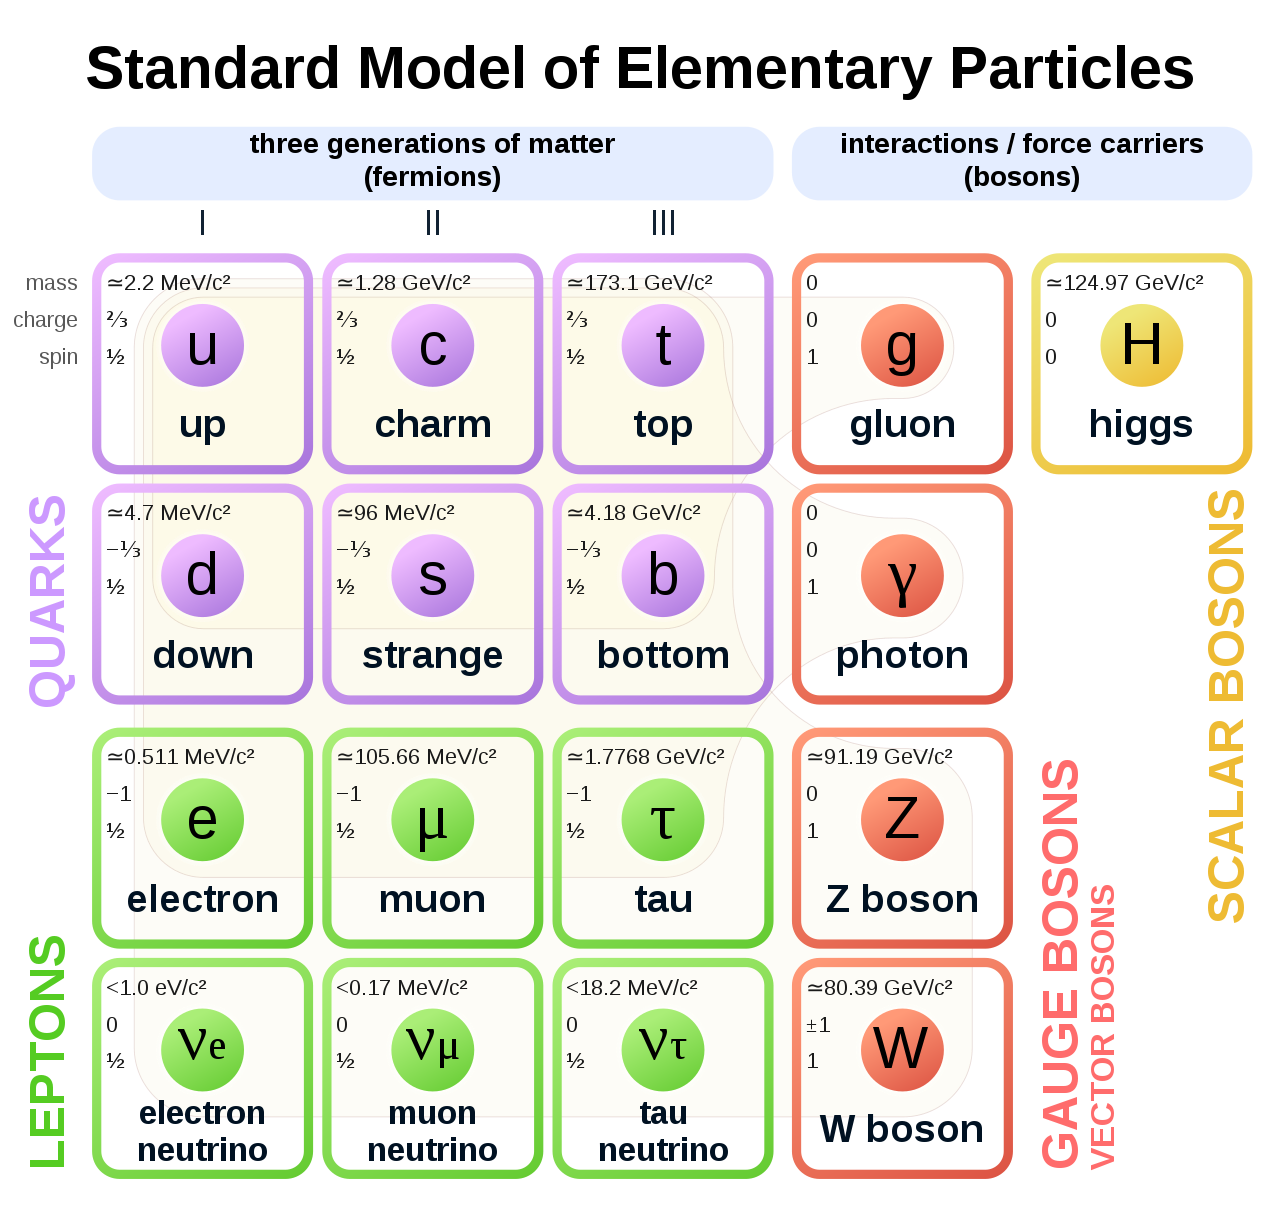
\includegraphics[width=12cm]{SM_sum.png}
\caption{\label{fig:SM_summary}
Summary of the SM elementary particles \cite{SM_summary} .}
\end{figure}
In figure \ref{fig:SM_summary}, the particles that are denoted by purple and green colors represent the matter fields. The red color represents the spin-one gauge bosons. The color yellow represents the Higgs boson. \par

\section{Symmetries in particle physics}\label{symmetry}
Symmetry transformation is an operation that can be performed on a particular system, which leaves the system invariant. The symmetries are important because they provide the conservation laws that govern the dynamics of the system. In particular, Noether's theorem connects the symmetries with the corresponding conservation laws \cite{Noether:1918zz}. For example, Noether's theorem connects the space and time translation symmetries to energy and momentum conservation, respectively \cite{Griffiths:2008zz}. \par
\subsection{Discrete symmetries}
Discrete symmetries are associated with the non-continuous change of the system. Under the discrete transformations, the system suddenly changes from one state to another. In particle physics, three important discrete symmetries govern the interactions, and they are known as \textit{parity} (P), \textit{charge conjugation} (C) and \textit{time reversal} (T).\par
The parity symmetry implies that the physical processes are invariant under flipping of the sign of space coordinates. This can be used to test whether the fundamental interactions are invariant under parity. The experimental evidence implies that the electromagnetic and strong interaction are invariant under parity. However, the weak interaction does not preserve the parity invariance \cite{Lee:1956qn}. \par
The charge conjugation transformation changes the sign of all the electromagnetic charges in the system. This implies an operator that changes the particle into an anti-particle. The strong and electromagnetic interaction both preserve charge conjugation, whereas the weak interaction does not remain invariant under C.\par
The time reversal symmetry implies that the invariance of the physical processes under the reversal of time. For example, under the T transformation a particle moving from point $A$ to $B$ along a certain path will reverse its direction from $B$ to $A$ on the same path \cite{Peccei:1998jv}. The time reversal operator is an anti-unitary operator. This means the $T$ operators act on quantum numbers as well as the operators \cite{Peskin:1995ev}, which provides
\begin{eqnarray}
T(\mathrm{c}-\text { number })\psi=(\mathrm{c}-\text { number })^{*} T\psi
\end{eqnarray}
\subsection{Continuous symmetries}
Continuous transformations gradually change the system from its original state to another. These continuous transformations play an important role in understanding elementary particle interactions. 
The elementary particle fields are defined using the complex-valued mathematical spaces. Under the continuous symmetries, the physical process remains invariant when the fields are rotated. 
For instance, electromagnetic interaction is invariant when the fields are rotated by a complex phase $e^{i\alpha}$, where $\alpha$ is a real number. This symmetry is known as $U(1)$ symmetry, and it is an abstract internal symmetry of the electromagnetic field. Similarly, the massless weak boson and fermion fields satisfy another abstract symmetry called $SU(2)_L$. These symmetries are based on the field rotations of two and three-dimensional spaces.\par
As the Yang-Mills theory \cite{Yang:1954ek} points out, the associated Lagrangian for these interacting fields should be invariant under local gauge transformations. This means the Lagrangian remains the same after an internal rotation. However, this theory seems to work well only for massless gauge fields such as photon field and gluon field. The heavy vector bosons, such as $W$ and $Z$, require another mechanism to generate their masses. For this, a scalar field called \textit{Higgs} field is employed.\par
Unlike the other fields, the lowest energy state of the Higgs field is a vacuum state (a state free of excitations) with non zero field value $v$, where $v$ is known as the vacuum expectation value (vev). Thus, the system spontaneously chooses a new vacuum. This makes the ground state only posses a subset of the symmetries of Lagrangian. This process is known as \textit{spontaneous symmetry breaking}. The broken Higgs field provide the source for the accumulation of mass for massless fermion and boson fields (see section \ref{higgssec}) \cite{Lancaster:2014pza}.\par
The standard model is specified by the special unitary group $SU(3)_c\times SU(2)_L\times U(1)_Y$. QCD has non-abelian gauge symmetry called $SU(3)_C$, the weak and electromagnetic interactions exhibit $SU(2)_L\times U(1)_Y$ symmetry.  As stipulated by the Higgs mechanism, the $SU(2)_L\times U(1)_Y$ breaks to electromagnetic subgroup $U(1)_{EM}$. The coupling for strong, weak, and electromagnetic interactions are given by $g_s$ for strong interaction, $g'$ for weak hypercharge $U(1)_Y$, and $g$ for weak isospin $SU(2)_L$. $ Y$ denotes the generator of week hypercharge, and the three generators of week isospin are given by $\tau^i$ where $i=1,2,3$. For the $SU(3)_C$, there are eight generators, which are denoted by $T^a$, where $a=1,...,8$. Since the interactions between these fields have a complex structure, it is easier to divide the SM Lagrangian into several sectors for the following analysis.

\section{Constructing the SM Lagrangian}
\subsection{The gauge sector}
The gauge field for strong interactions are given by $G_{\mu}^a$, for the $SU(2)_L$ the gauge field is given by $W_{\mu}^i$ and the gauge field for the $U(1)_Y$ is given by $B_{\mu}$. The corresponding abelian/non-abelian field strength tensors for these gauge fields are given as follows:
\begin{eqnarray}\label{GaugeFieldStreangth}
\begin{aligned} B_{\mu \nu} &=\partial_{\mu} B_{\nu}-\partial_{\nu} B_{\mu} \\ W_{\mu \nu}^{i} &=\partial_{\mu} W_{\nu}^{i}-\partial_{\nu} W_{\mu}^{i}-g \epsilon^{i j k} W_{\mu}^{j} W_{\nu}^{k} \\ G_{\mu \nu}^{a} &=\partial_{\mu} G_{\nu}^{a}-\partial_{\nu} G_{\mu}^{a}-g_{s} f^{a b c} G_{\mu}^{b} G_{\nu}^{c} \end{aligned}
\end{eqnarray}
In the SM Lagrangian gauge sector is realized as follows:
\begin{eqnarray}
\mathcal{L}_{\mathrm{gauge}}=-\frac{1}{4} B_{\mu \nu} B^{\mu \nu}-\frac{1}{4} W_{\mu \nu}^{i} W^{i, \mu \nu}-\frac{1}{4} G_{\mu \nu}^{a} G^{a, \mu \nu}
\end{eqnarray}
\subsection{The fermionic sector}
The fermionic sector contains the matter fields. Also, it exhibits the $SU(2)_L\times U(1)_Y$ symmetry, which accounts the weak and electromagnetic  interactions. There are three generations of fermions each consist of \textit{neutrino} ($v_i$) with electromagnetic charge $Q_i=0$, \textit{lepton} ($l_i$) with $Q_i=-1$, up type \textit{quark} with $Q_i=+2/3$ and down type quark with $Q_i=-1/3$. The $SU(2)_L$ determines the transformation properties of these fermion fields under weak charge. These fields are arrange as a $2\times 1$ column vector. This is known as \textbf{2} representation. For an example, $u_L$ and $d_L$ together form \textbf{2} representation of $SU(2)_L$. Similarly, $v_{eL}$ and $e_L$ also transform together to form doublet. On the other hand, right handed fields transform as singlets under $SU(2)_L$.\par
The representation of $U(1)_Y$ is the \textit{hypercharge} of the field. The hypercharge is assigned based on the final electromagnetic charge of the fermion. The representation of $SU(3)_C$ is determined by the color charge. The left and right handed quarks comes in three colors as $3\times 1$ column vector. This is the \textbf{3} representation in $SU(3)_C$. Leptons do not carry a color. They are in the singlet representation of $SU(3)_C$.
Altogether, for an example, the transformation of up type quark under $SU(3)_c\times SU(2)_L\times U(1)_Y$ is
\begin{eqnarray}
u_L\sim (3,2,\frac{1}{3})
\end{eqnarray}
The interaction between the matter and gauge fields is captured by the covariant derivative.
\begin{eqnarray}
D_{\mu}=\partial_{\mu}+i g^{\prime} B_{\mu} Y+i g W_{\mu}^{i} \tau^{i}+i g_{s} G_{\mu}^{a} T^{a}
\end{eqnarray} 
Using this the fermionic part of the standard model Langrangian can be written as:
\begin{eqnarray}
\mathcal{L}_{\text{fermionic}}=\sum_{i=1}^{3}\left(\bar{E}^i_L i \slashed{D}E_{L}^i+\bar{Q}_{L}^i i\slashed{D}Q_L^i+\bar{e}_R^i i\slashed{D}e_{R}^i+\bar{u}_R^i i\slashed{D}u_R^i+\bar{d}_R^i i\slashed{D}d_R^i\right)
\end{eqnarray}
where 
\begin{eqnarray}
\begin{aligned} E_{L}^{i} &=P_{L}\left(\begin{array}{c}{\nu_{i}} \\ {e_{i}}\end{array}\right)=\left(\left(\begin{array}{c}{\nu_{e}} \\ {e}\end{array}\right)_{L},\left(\begin{array}{c}{\nu_{\mu}} \\ {\mu}\end{array}\right)_{L},\left(\begin{array}{c}{\nu_{\tau}} \\ {\tau}\end{array}\right)_{L}\right) \\ Q_{L} &=P_{L}\left(\begin{array}{c}{u_{i}} \\ {d_{i}}\end{array}\right)=\left(\left(\begin{array}{c}{u} \\ {d}\end{array}\right)_{L},\left(\begin{array}{c}{c} \\ {s}\end{array}\right)_{L},\left(\begin{array}{c}{t} \\ {b}\end{array}\right)_{L}\right), \end{aligned}
\end{eqnarray}
$P_{L / R}=\left(1 \mp \gamma^{5}\right) / 2$.\\
%Lagrangian density can be devided into couple of sections as follows.
\subsection{Higgs sector}\label{higgssec}
As discussed in the section \ref{symmetry}, the Higgs field is needed as a mass generating mechanism to heavy vector bosons. The Lagrangian is \cite{Manohar:2000dt, Lancaster:2014pza, LlewellynSmith:1973yud}: 
\begin{eqnarray}\label{higgsLagrangian}
\mathcal{L}_{\mathrm{H}}=\left(D_{\mu} \phi\right)^{\dagger}\left(D^{\mu} \phi\right)+\frac{1}{2}\mu^{2} \phi^{\dagger} \phi-\frac{1}{4}\lambda\left(\phi^{\dagger} \phi\right)^{2}+\mathcal{L}_{gauge}
\end{eqnarray}
where 
\begin{eqnarray}
\langle\phi\rangle=\left(\begin{array}{l}{\phi^+} \\ {\phi^0}\end{array}\right)=\frac{1}{\sqrt{2}}\left(\begin{array}{l}{\phi_3+i\phi_4} \\ {\phi_1+i\phi_2}\end{array}\right)
\end{eqnarray}
Here $\mu$ and $\lambda$ are both real parameters. However, the minimum of the Higgs potential is not at $\langle\phi\rangle=0$. Thus, the  potential term provides the spherical shell of minima at a radius $v=\left(\frac{\mu^2}{\lambda}\right)^{\frac{1}{2}}$. On the surface of this spherical shell there are infinitely many equivalent vacua. The Higgs field spontaneously pick one of these vacua and breaks the symmetry. For simplicity, consider the following vacuum field configuration:
\begin{eqnarray}
(\phi_1^0)^2=\frac{2\mu^2}{\lambda}=2 v^2, \text{  } \phi_2^0=0\text{  }\phi_3^0=0\text{  }\phi_4^0=0
\end{eqnarray}
More concisely, 
\begin{eqnarray}\label{higgsvcuum}
\langle\phi\rangle=\left(\begin{array}{l}{0} \\ {v}\end{array}\right)
\end{eqnarray}
The symmetry breaking $SU(2)_L\times U(1)_Y\rightarrow U(1)_Q$ does not break all the symmetries. For instance, our choice of vacuum given in equation (\ref{higgsvcuum}) is still invariant under $\hat{U}=e^{i(\frac{Y}{2}+I_3\tau^3)\alpha(x)}$ transformation. In fact $Q=\frac{Y}{2}+I_3$ where $Q$ is the electromagnetic charge. Using this the above transformation can be written as  $\hat{U}=e^{iQ\alpha(x)}$. According to the \textit{Yang-Mills} theory this is equivalent to a U(1) transformation. Therefore, the electromagnetic interaction emerges unbroken from this symmetry breaking. \par
The excitation above the vacuum state of the Higgs field is given below:
\begin{eqnarray}
\phi(x)=\left(\begin{array}{l}{\quad 0} \\ {v+\frac{h(x)}{\sqrt{2}}}\end{array}\right)
\end{eqnarray}
The first term in the Higgs Lagrangian becomes
\begin{eqnarray}
(D_{\mu}^{\dagger}\phi)(D^{\mu}\phi)=\frac{1}{2}(\partial_{\mu}h(x))^2+\frac{g^2v^2}{4}(W_{\mu}^1)^2+\frac{g^2v^2}{4}(W^2_{\mu})^2+\frac{v^2}{4}(g W_{\mu}^3-g'B_{\mu})^2
\end{eqnarray}
Note that the mass term of a spin-1 field has the form $\frac{1}{2}(mass)^2\times(field)^2$. Following from this, the $W_{\mu}^1$ and $W_{\mu}^2$ fields obtain a mass $M^2_W=\frac{g^2v^2}{2}$. The linear combination of the fields $(g W_{\mu}^3-g'B_{\mu})$ also becomes massive. The Higgs field components $\phi_2,\phi_3$ and $\phi_4$ disappeared from the interaction Lagrangian. The massive excitation of the scalar field is known as \textit{Higgs} boson.\par
The linear combination $g'W^3_{\mu}+gB_{\mu}$ does not appear in the above Lagrangian. Therefore, this combination is identified as the massless photon field. The \textit{Weinberg angle} is defined as the ratio of coupling constants $g$ and $g'$ as $\tan \theta_W=\frac{g'}{g}$. Using this angle two new fields are defined as:
\begin{eqnarray}
\left(\begin{array}{l}{Z_{\mu}} \\ {A_{\mu}}\end{array}\right)=\begin{pmatrix} 
\cos\theta_W & -\sin\theta_W \\
\sin\theta_W & \cos\theta_W 
\end{pmatrix}\left(\begin{array}{l}{W_{\mu}^3} \\ {B_{\mu}}\end{array}\right)
\end{eqnarray}  
where $Z_{\mu}$ is the $Z$ boson field and $A_{\mu}$ is the photon field.
\subsection{Yukawa sector}
The Higgs couplings to the fermions in the SM is described by the \textit{Yukawa} Lagrangian. The Lagrangian needs to be \textit{Lorentz invariant} and have mass dimension 4. Its general form is
\begin{eqnarray}
\mathcal{L}_{\mathrm{Yukawa}} \ni -y_{\psi}\bar{\psi}_R\phi\psi_L+ \mbox{c.c},
\end{eqnarray} 
where $\psi$ and $\phi$ are fermion field and scalar field respectively. $y_{\psi}$ is the dimensionless coupling between the scalar and fermion fields, which is known as the \textit{Yukawa coupling}.
\subsubsection{Lepton sector}
\vspace{-0.3cm}
Using the above definition, the Yukawa term in the Lagrangian can be obtained for the $SU(2)_L$ doublet $E_{L}=\left(\nu_{L}, e_{L}\right)^{T}$ as follows:
\begin{eqnarray}
\mathcal{L}_{\mathrm{Yukawa}} \ni-\left[y_{e} \overline{e}_{R} \Phi^{\dagger} E_{L}+y_{e}^{*} \overline{E}_{L} \Phi e_{R}\right]
\end{eqnarray}
The coupling $y_{e}$ is obtained using
\begin{eqnarray}
\frac{y_{e}}{\sqrt{2}}=\frac{m_{e}}{v}
\end{eqnarray} 	
Also, this can be extended to all three generations in SM. This gives a generalized lepton sector as
\begin{eqnarray}
\mathcal{L}_{\mathrm{lepton}} \ni -\left[Y_{ij} \overline{e}_{Rj} \Phi^{\dagger} E_{Li}+Y_{ij}^{*} \overline{E}_{Li} \Phi e_{Rj}\right],
\end{eqnarray} 
where $Y_{ij}$ is the matrix element of the Yukawa matrix.
Due to the absence of $\nu_{Ri}$ fields, in SM $neutrinos$ do not couple to Higgs field. The neutrinos do not get their mass from the Higgs mechanism.
\vspace{-0.3cm}
\subsubsection{Quark sector}
\vspace{-0.3cm}
Similarly, the Yukawa interaction between $SU(2)_L$ quark doublet $Q_L=\left(u_{L}, d_{L}\right)^{T}$ and down type quark singlet $d_R$ can be written as 
\begin{eqnarray}\label{downType}
\mathcal{L}_{\mathrm{Yukawa}} \ni-\left[y_{d} \overline{d}_{R} \Phi^{\dagger} Q_{L}+y_{d}^{*} \overline{Q}_{L} \Phi d_{R}\right]
\end{eqnarray}
The mass generation of up type quarks is obtained by using the conjugate doublet transformation in $SU(2)$. The conjugate Higgs doublet is given by
\begin{eqnarray}
\tilde{\phi} \equiv i \sigma^{2} \phi^{*}=i\left(\begin{array}{cc}{0} & {-i} \\ {i} & {0}\end{array}\right)\left(\begin{array}{c}{\phi^{-}} \\ {\phi^{0 *}}\end{array}\right)=\left(\begin{array}{c}{\phi^{0 *}} \\ {-\phi^{-}}\end{array}\right)
\end{eqnarray}
As an artifact of this, we obtain $Y=-\frac{1}{2}$. Using this, another gauge invariant term can be obtained,
\begin{eqnarray}\label{upType}
\mathcal{L}_{\mathrm{Yukawa}} \ni-\left[y_{u} \overline{u}_{R} \tilde{\phi}^{\dagger} Q_{L}+y_{u}^{*} \overline{Q}_{L} \tilde{\phi} u_{R}\right]
\end{eqnarray}
As shown before, the quark masses and the Higgs vev determine the Yukawa couplings.  This can also be generalized to all 3 generations of quarks as well. The complete Yukawa term,
 \begin{eqnarray}\label{SMYukawa}
 -\mathcal{L}_{\mathrm{Yukawa}}=Y_{i j}^{d} \overline{Q}_{L i} \phi d_{R j}+Y_{i j}^{u} \overline{Q}_{L i} \tilde{\phi} u_{R j}+Y_{i j}^{e} \overline{E}_{L i} \phi e_{R j}+\mathrm{h.c.}
 \end{eqnarray}
Also, this term is the source of all \textit{flavor} interactions \cite{Isidori:2010kg}. 
\subsection{The Standard Model Lagrangian}
Considering all the possible interactions between the gauge bossons, fermions and scalars the final Lagrangian that describes the SM can be written as follows: 
\begin{eqnarray}\label{SMLagarangian}
\mathcal{L}_{\mathrm{SM}}=\mathcal{L}_{\text { fermionic + gauge }}+\mathcal{L}_{\text { Higgs }}+\mathcal{L}_{\text { Yukawa }}.
\end{eqnarray}
In the table \ref{tab:consti_SM} we summarize all the SM constituents and their corresponding gauge multiplets.
\begin{table}[H]
\caption{Constituents of the SM}\label{tab:consti_SM}
\begin{center}
\begin{tabular}{ |c|c|c|c| } 
\hline
Type\quad spin & Field & Multiplet \\ 
\hline
\multirow{3}{4em}{Vector\, 1} & $B_{\mu}$ & (1,1,0) \\ 
& $W_{\mu}$ & (1,3,0) \\ 
& $G_{\mu}$& (8,1,0) \\ 
\hline
\multirow{5}{4em}{Spinor\, $\frac{1}{2}$} & $E_{Li}$ & (1,2,$-\frac{1}{2}$) \\ 
& $Q_{Li}$ & (3,2,$\frac{1}{6}$) \\ 
& $e_{Ri}$& (1,1,-1) \\ 
& $u_{Ri}$ & (3,1,$\frac{2}{3}$) \\
& $d_{Ri}$ & (3,1,$-\frac{1}{3}$) \\
\hline
Sacalar\quad 0 & $\phi$ & (1,2,$\frac{1}{2}$)\\
\hline
\end{tabular}
\end{center}
\end{table}
\subsection{Cabibbo-Kobayashi-Maskawa (CKM) matrix}  
Consider equations (\ref{downType}) and (\ref{upType}). They can be generalized to all three generations of quarks in the SM.
\begin{eqnarray}
\mathcal{L}_{\mathrm{Yukawa}}^{\text{quark}}=-\sum_{i=1}^{3} \sum_{j=1}^{3}\left[y_{i j}^{u} \bar{u}_{R i} \tilde{\phi}^{\dagger} Q_{L j}+y_{i j}^{d} \bar{d}_{R i} \phi^{\dagger} Q_{L j}\right]+\mathrm{h.c.}
\end{eqnarray}
The dimensionless \textit{Yukawa} couplings now become $3\times3$ matrices. These matrices contain 18 complex parameters. As shown in the section \ref{higgssec}, replacing the Higgs by its vacuum configuration $\phi=(0, v/\sqrt{2})^T$ provides the mass term. 
\begin{eqnarray}
\mathcal{L}_{\mathrm{Yukawa}}^{q} \supset-\left(\bar{u}_{1}, \bar{u}_{2}, \bar{u}_{3}\right)_{R} \mathcal{M}^{u}\left(\begin{array}{c}{u_{1}} \\ {u_{2}} \\ {u_{3}}\end{array}\right)_{L}-\left(\bar{d}_{1}, \bar{d}_{2}, \bar{d}_{3}\right)_{R} \mathcal{M}^{d}\left(\begin{array}{c}{d_{1}} \\ {d_{2}} \\ {d_{3}}\end{array}\right)_{L}+\mathrm{h.c.},
\end{eqnarray}
where 
\begin{eqnarray}
\mathcal{M}_{i j}^{u}=\frac{v}{\sqrt{2}} y_{i j}^{u}, \quad \mathcal{M}_{i j}^{d}=\frac{v}{\sqrt{2}} y_{i j}^{d}.
\end{eqnarray}
The $\mathcal{M}_{i j}^{u}$ and $\mathcal{M}_{i j}^{d}$ are known as the quark mass matrices in the \textit{generation} space. The diagonalization of these mass matrices provide the quark mass eiganstates. This is done by multiplying the mass matrices by unitary matrices $U_{L}, U_{R}, D_{L}$ and $D_{R}$. They are defined by
\begin{eqnarray}
\left(\begin{array}{c}{u_{1}} \\ {u_{2}} \\ {u_{3}}\end{array}\right)_{L, R}=U_{L, R}\left(\begin{array}{c}{u} \\ {c} \\ {t}\end{array}\right)_{L, R}, \quad\left(\begin{array}{c}{d_{1}} \\ {d_{2}} \\ {d_{3}}\end{array}\right)_{L, R}=D_{L, R}\left(\begin{array}{c}{d} \\ {s} \\ {b}\end{array}\right)_{L, R},
\end{eqnarray}
where $u,c,t,d,s$ and $b$ are quark mass eigenstates. This gives us the diagonalized mass matrices. 
\begin{eqnarray}
U_{R}^{-1} \mathcal{M}^{u} U_{L}=\left(\begin{array}{ccc}{m_{u}} & {0} & {0} \\ {0} & {m_{c}} & {0} \\ {0} & {0} & {m_{t}}\end{array}\right), \quad D_{R}^{-1} \mathcal{M}^{d} D_{L}=\left(\begin{array}{ccc}{m_{d}} & {0} & {0} \\ {0} & {m_{s}} & {0} \\ {0} & {0} & {m_{b}}\end{array}\right).
\end{eqnarray}
Also, $\mathcal{M}^u$ and $\mathcal{M}^d$ diagonalizes \textit{Yukawa} matrices $y_{i j}^{u}=\frac{\sqrt{2}}{v} \mathcal{M}_{i j}^{u} \text { and } y_{i j}^{d}=\frac{\sqrt{2}}{v} \mathcal{M}_{i j}^{d}$.\par
These mass eigenstates (physical states) of up and down type quarks can be coupled in charged current interactions.
\begin{eqnarray}
J_{L}^{+\mu}=\left(\bar{u}_{1}, \bar{u}_{2}, \bar{u}_{3}\right)_{L} \gamma^{\mu}\left(\begin{array}{c}{d_{1}} \\ {d_{2}} \\ {d_{3}}\end{array}\right)=(\bar{u}, \bar{c}, \bar{t})_{L} U_{L}^{\dagger} \gamma^{\mu} D_{L}\left(\begin{array}{c}{d} \\ {s} \\ {b}\end{array}\right)_{L}=(\bar{u}, \bar{c}, \bar{t})_{L} \gamma^{\mu} V\left(\begin{array}{c}{d} \\ {s} \\ {b}\end{array}\right)_{L}.
\end{eqnarray} 
Here $V=U_{L}^{\dagger}D_{L}$ is known as the \textit{Cabibbo-Kobayashi-Maskawa} (CKM) matrix, and  it is given by 
\begin{eqnarray}
V_{\text{CKM}}=\left(\begin{array}{ccc}{V_{u d}} & {V_{u s}} & {V_{u b}} \\ {V_{c d}} & {V_{c s}} & {V_{c b}} \\ {V_{t d}} & {V_{t s}} & {V_{t b}}\end{array}\right).
\end{eqnarray}
The CKM is unitary 
\begin{eqnarray}
V^{\dagger} V=\left(U_{L}^{\dagger} D_{L}\right)^{\dagger}\left(U_{L}^{\dagger} D_{L}\right)=D_{L}^{\dagger} U_{L} U_{L}^{\dagger} D_{L}=1
\end{eqnarray}
Since the CKM matrix is a $3\times 3$ matrix it is defined by nine complex parameters (18 real numbers). The constraint $V_{a b}^{\dagger} V_{b c}=\delta_{a c}$ reduce this to nine real parameters. The redefinition $q_{L} \rightarrow e^{i\alpha_{q_L}} q_{L}$ can technically remove six phases because there are six different quark fields. However, the common phase redefinition of all the quarks does not affect the CKM matrix. This, in turn, reduces the number of nonphysical phases to five. Altogether, there are $9-5=4$ independent parameters to describe the CKM matrix. There is no unique parameterization for the CKM matrices. The most common ones are `` Standard parametarization" \cite{Chau:1984fp} and ``Wolfenstein parameterization"\cite{Wolfenstein:1983yz}. 
\vspace{-0.3cm}
\subsubsection{Standard Parameterization }
\vspace{-0.3cm}
The Standard parameterization is given by
\begin{eqnarray}
V_{\text{CKM}}=\left(\begin{array}{ccc}{c_{12} c_{13}} & {s_{12} c_{13}} & {s_{13} e^{-i \delta}} \\ {-s_{12} c_{23}-c_{12} s_{23} s_{13} e^{i \delta}} & {c_{12} c_{23}-s_{12} s_{23} s_{13} e^{i \delta}} & {s_{23} c_{13}} \\ {s_{12} s_{23}-c_{12} c_{23} s_{13} e^{i \delta}} & {-s_{23} c_{12}-s_{12} c_{23} s_{13} e^{i \delta}} & {c_{23} c_{13}}\end{array}\right),
\end{eqnarray}
where $s_{ij}=\sin\theta_{ij}$ and $c_{ij}=\cos\theta_{ij}(i=1,2,3)$. The phase $\delta$ is necessary for the CP violation, and its range $0\leq \delta\leq 2\pi$. The measurements of CPV in $K$ decays constrain this range to $0\leq \delta\leq \pi$ \cite{Buras:1998raa}.\par
The $s_{13}$ and $s_{23}$ are in the order of $10^{-3}$, and $c_{13}=c_{23}=1$ \cite{Tanabashi:2018oca}. This leaves 4 independent parameters 
\begin{eqnarray}
s_{12}=\left|V_{u s}\right|, \quad s_{13}=\left|V_{u b}\right|, \quad s_{23}=\left|V_{c b}\right|, \quad \delta
\end{eqnarray}
\subsubsection{Wolfenstein Parameterization}
\vspace{-0.2cm}
The Wolfenstein Parameterization can be obtained by expressing the independent parameters in standard parameterization by $\lambda, A, \rho, \eta$ \cite{Buras:1994ec}.
\begin{eqnarray}
s_{12}=\lambda, \quad s_{23}=A \lambda^{2}, \quad s_{13} e^{-i \delta}=A \lambda^{3}(\varrho-i \eta)
\end{eqnarray}
This is an approximate parameterization, in which each CKM elements is expanded in power series of small parameter $\lambda = |V_{us}|=0.22$. This gives us 
\begin{eqnarray}
\hat{V}=\left(\begin{array}{ccc}{1-\frac{\lambda^{2}}{2}} & {\lambda} & {A \lambda^{3}(\varrho-i \eta)} \\ {-\lambda} & {1-\frac{\lambda^{2}}{2}} & {A \lambda^{2}} \\ {A \lambda^{3}(1-\varrho-i \eta)} & {-A \lambda^{2}} & {1}\end{array}\right)+\mathcal{O}\left(\lambda^{4}\right).
\end{eqnarray}
\subsubsection{Unitarity triangles}
\vspace{-0.2cm}
Unitarity relationships can be expressed by triangle relations defined in a complex plane. For example, 
\begin{eqnarray}
\begin{array}{l}{V_{u d} V_{u b}^{*}+V_{c d} V_{c b}^{*}+V_{t d} V_{t b}^{*}=0} \\ {V_{u  s} V_{u  b}^{*}+V_{c s} V_{c b}^{*}+V_{t s} V_{t b}^{*}=0} \\ {V_{u d } V_{u s}^{*}+V_{c d} V_{c s}^{*}+V_{t d} V_{t s}^{*}=0} \\ {V_{u d} V_{t d}^{*}+V_{u s} V_{t s}^{*}+V_{u b} V_{t b}^{*}=0} \\ {V_{c d} V_{t d}^{*}+V_{c s} V_{t s}^{*}+V_{c b} V_{t b}^{*}=0} \\ {V_{u d } V_{c d}^{*}+V_{u s} V_{c s}^{*}+V_{u b} V_{c b}^{*}=0}\end{array}
\end{eqnarray}
The area of the unitarity triangles provide the measurement of CP violation. This measurement is obtained by\cite{Jarlskog:1988ii} 
\begin{eqnarray}
\left|J_{\mathrm{CP}}\right|=2 \cdot A_{\Delta}
\end{eqnarray}
where $|J_{CP}|$ is the \textit{Jarlskog invarient} and $A_{\Delta}$ is the area of the unitarity triangle. Therefore, precise measurements of the CKM parameters along with these unitarity relationships gives us important information on CP violation. Also, unitarity triangles are important for understanding the flavor changing neutral current processes (see sec. \ref{fcnc}).
\subsection{Flavor physics}
In \textit{flavor physics}, the interactions between different flavors are studied extensively. Massless gauge bosons such as \textit{gluons} and \textit{photons} do not distinguish between different flavors. However, the weak and the Yukawa interactions are directly affected by the flavor of the participants in the interaction. When it comes to beyond the standard model interactions, there may be some new degrees of freedom that are affected by the flavors.\par
During a \textit{flavor changing} interaction, flavor quantum numbers change. There are two types of flavor changing interactions. If the interaction is between both up type and down type flavors or charged leptons and neutrinos, then it involves \textit{flavor changing charged current} (FCCC). For the interactions between either up type or down type flavors but not both and/or either charged leptons and neutrinos but not both, then it involves the \textit{flavor changing neutral currents} (FCNC). No term in the SM Lagrangian changes flavor in $Z^0, g$ and $\gamma$ interactions. Therefore, it makes FCNC are highly sensitive to the new physics.
\vspace{-0.5cm}
\subsubsection{Weak interactions}
\vspace{-0.3cm}
The weak interactions are summarized in the following form
\begin{eqnarray}
\mathcal{L}_{\mathrm{int}}^{\mathrm{EW}}=\mathcal{L}_{\mathrm{CC}}+\mathcal{L}_{\mathrm{NC}}
\end{eqnarray}
\vspace{-0.5cm}
where $\mathcal{L}_{CC}$ and $\mathcal{L}_{NC}$ describe the charged current and the neutral current interactions. In particular, the CC is given by \cite{Buras:1998raa}

\begin{eqnarray}
\mathcal{L}_{\mathrm{CC}}=\frac{g}{2 \sqrt{2}}\left(J_{\mu}^{+} W^{+\mu}+J_{\mu}^{-} W^{-\mu}\right),
\end{eqnarray}
where 
\begin{eqnarray}
J_{\mu}^{+}=J^1_{\mu}+iJ^2_{\mu}=\bar{U}_L\gamma_{\mu}D_L+\bar{l}\gamma_{\mu}\nu_{L},
\end{eqnarray}
$U_L$ is an up type quark, $D$ is a down type quark, $l$ is a lepton and $v$ is a neutrino.
The NC is given by
\begin{eqnarray}
\mathcal{L}_{\mathrm{NC}}=-e J_{\mu}^{\mathrm{em}} A^{\mu}+\frac{g}{2 \cos \theta_W} J_{\mu}^{0} Z^{\mu},
\end{eqnarray}
where $e$ is the QED coupling. The neutral electromagnetic and weak currents are given by
\begin{eqnarray}
\begin{array}{c}{J_{\mu}^{\mathrm{em}}=\sum_{f} Q_{f} \overline{f} \gamma_{\mu} f} \\ {J_{\mu}^{0}=\sum_{f} \overline{f} \gamma_{\mu}\left(v_{f}-a_{f} \gamma_{5}\right) f}\end{array}
\end{eqnarray}
where 
\begin{eqnarray}
v_{f}=T_{3}^{f}-2 Q_{f} \sin ^{2} \theta_W, \quad a_{f}=T_{3}^{f}.
\end{eqnarray}
The $Q_f$ and $T_3^f$ denotes the charge and the third component of the weak isospin of the left-handed fermion. The photonic and gluonic vertices are vector-like (V), the $W^{\pm}$ vertices involve only vector-axial minus vector-like $(V-A)$ and the $Z^0$ vertices involve both $V-A$ and $V+A$ structures. Also, the vertices that involve Higgs play an important role. This relates the CP-violating decays and transitions. 
\subsubsection{FCNC}\label{fcnc}
\vspace{-0.3cm}
At one loop order the possible FCNC interactions are summerized by triple and quartic effective vertices. In the literature these vertices are known as \textit{penguin} and \textit{box} diagrams. The name ``penguin" was coined by J.Ellis \cite{Ellis:1977uk}. Penguin diagrams are defined by a single exchange of a $W$ boson. Whereas, the box diagrams contain two $W$ exchanges. \par
The importance of the penguin diagrams was pointed out in the work of Vainshtein, Zakharov, and Shifman \cite{Shifman:1975tn}. For instance, penguin diagrams are responsible for the enhancement of the $\Delta I=1/2$ amplitude compared to the $\Delta I=3/2$ amplitude in weak $K\rightarrow \pi\pi$ decays. The importance of the penguins to CP violation was first pointed out by Bander, Silverman and Soni 
\cite{Bander:1979px}. They showed that the interference between the tree level diagrams and the penguin diagrams can give a large CP asymmetry in $B$ decays.\par
In $b$ transitions to lighter quarks such as $s$ and $d$, the penguin effects are rather pronounced. In these penguins the $t$ quark is primarily contributing to the loop. This is because the amplitude of the penguin is proportional to the kinematic factor $(m_q/M_W)^2$ and $(m_t/M_W)^2\gg (m_{c,u}/M_W)^2$ (see sec \ref{GIM}). Also, there is a large coupling between $b$ and $t$ because $|V_{tb}|\sim 1$. This feature of $b$ penguins makes $b\rightarrow s$ and $b\rightarrow d$ transitions sensitive to $|V_{ts}|$ and $|V_{td}|$. \par
In particular, the decays such as $b\rightarrow s (d)$ are classified into a class of diagrams that are known as \textit{electromagnetic penguins}. In these decays a hard photon is emitted from a charged particle. This hard photon is an excellent experimental signature.  The Feynman diagram for $b\rightarrow s,d \gamma$ transition is given in figure \ref{fig:Btosd_fcnc}.
\vspace*{-0.5cm}
\begin{figure}[H]
\centering
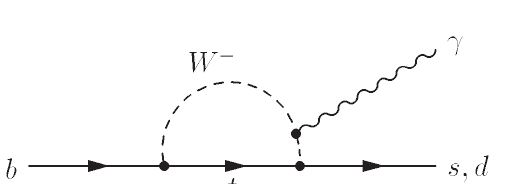
\includegraphics[width=8cm]{em_peng.JPG}
\caption{\label{fig:Btosd_fcnc}
The electromagnetic penguin diagram \cite{Lingel:1998fa}.}
\end{figure}
The figure \ref{fig:Btosd_fcnc} shows that the $b\rightarrow s,d \gamma$ transition is a loop suppressed process. In the SM there exist no tree level diagrams for these FCNC transitions. 
\subsection{GIM mechanism}\label{GIM}
The suppression of the $b\to s(d)$ was further explained by the Glashow-Illiopoulos-Maiani (GIM) mechanism. The amplitude of figure \ref{fig:Btosd_fcnc} is given by \cite{Grinstein:2017pvg}
\begin{eqnarray}
\mathcal{M}=e q_{\mu} \epsilon_{\nu} \bar{u}\left(p_{s}\right) \sigma^{\mu \nu}\left(\frac{1+\gamma_{5}}{2}\right) u\left(p_{b}\right) \frac{m_{b}}{M_{W}^{2}} \frac{g^{2}}{16 \pi^{2}} \cdot I,
\end{eqnarray}
where 
\begin{eqnarray}\label{btos_amp_factor}
I=\sum_{i=u, c, t} V_{i b} V_{i s}^{*} F\left(\frac{m_{i}^{2}}{M_{W}^{2}}\right).
\end{eqnarray}
The term $\frac{g^2}{16\pi^2}$ is a loop factor, and it can be given as $\frac{g^{2}}{16 \pi^{2}} \sim \frac{\alpha}{4 \pi \cos^2\theta_{W}}$. We insert the $b$ quark mass $m_b$ to flip the chirality of the $b$ quark.\par
In equation (\ref{btos_amp_factor}), the function $F(x)$ arises by the explicit calculation of the diagram. Since $m_t\gg M_W$, we cannot safely Taylor expand the function $F(m_i/M_W)$. The function $I$ is invariant under $F(x)\to F(x)+ \mbox{constant}$ from the unitarity of the CKM matrix. Under this transformation $F(0)=0$ without loss of generality. Besides, the unitarity of the CKM matrix elements provide $V_{t b} V_{t s}^{*}=-\sum_{i=u, c} V_{i b} V_{i s}^{*}$. Following from this, we obtain
\begin{eqnarray}
I=-V_{c b} V_{c s}^{*}\left(F\left(\frac{m_{t}^{2}}{M_{W}^{2}}\right)-F(\frac{m_{c}^{2}}{M_{W}^{2}}) \right)-V_{u b} V_{u s}^{*}\left(F\left(\frac{m_{t}^{2}}{M_{W}^{2}}\right)-F(\frac{m_{u}^{2}}{M_{W}^{2}}) \right).
\end{eqnarray}
Since $m_u, m_c\ll M_W$, the term $F(m_{u,c}^2/M_W^2)$ can be expanded in Taylor series. This gives
\begin{eqnarray}
\begin{aligned}
I &=-V_{c b} V_{c s}^{*}\left(F\left(\frac{m_{t}^{2}}{M_{W}^{2}}\right)-F^{\prime}(0) \frac{m_{c}^{2}}{M_{W}^{2}}\right)-V_{u b} V_{u s}^{*}\left(F\left(\frac{m_{t}^{2}}{M_{W}^{2}}\right)-F^{\prime}(0) \frac{m_{u}^{2}}{M_{W}^{2}}\right)+\cdots \\
&=F\left(\frac{m_{t}^{2}}{M_{W}^{2}}\right) V_{t b} V_{t s}^{*}+F^{\prime}(0) \sum_{i=u, c} V_{i b} V_{i s}^{*} \frac{m_{i}^{2}}{M_{W}^{2}}+\cdots \\
& \sim \epsilon^{2} F\left(\frac{m_{t}^{2}}{M_{W}^{2}}\right),
\end{aligned}
\end{eqnarray}
where $\epsilon^{2}=A\lambda^2$ in the Wolfenstein parameterization. The combination of loop suppression, mass suppression and CKM suppression is provided by GIM mechanism. As a result, the FCNC are highly suppressed in the SM. Also, the contribution from $F(m_u^2/M_W^2)$ and $F(m_c^2/M_W^2)$ is negligible compared to the $F(m_t^2/M_W^2)$. Thus, the virtual top quark exchanges dominate the $b\to s(d)$ amplitude.
\subsection{Effective weak interactions}
In the SM, the coupling of the $W^{\pm}$ bosons to the fermions are the only flavor changing interactions \cite{Neubert:2005mu}. At low energies, i.e. $E\ll M_W$, we can ignore the effects of the heavy bosons. This is known as integrating out of the heavy degrees of freedom (see sec \ref{sec:HQET}). As a result, a full SM interaction is converted into a local four fermion interaction. The effective Lagrangian can be expressed by a series of effective vertices and their effective coupling constants (see sec \ref{section:OPE_b}). These \textit{effective coupling} constants provide the short distant (high energy) physics, and they are known as Wilson coefficients ($C_i$). The long distant (low energy) physics is given by effective operators $\langle Q_i \rangle$. Since the Wilson coefficients are associated with high energy scales, where $\frac{\alpha_s}{\pi}\sim 0.1$, they can be perturbatively expanded in $\alpha_s$. This is because at high energy scales the $C_i$ are obtained by matching the effective diagrams with the full theory diagrams at the weak scale ($\mu\sim M_W$). For example, the explicit form of the first two Wilson coefficients are \cite{Neubert:2005mu}
\begin{eqnarray}\label{C1C2_will_co}
\begin{array}{l}
C_{1}(\mu)=1+\frac{3}{N_{c}} \frac{\alpha_{s}(\mu)}{4 \pi}\left(\ln \frac{M_{W}^{2}}{\mu^{2}}-\frac{11}{6}\right)+O\left(\alpha_{s}^{2}\right) \\
C_{2}(\mu)=-3 \frac{\alpha_{s}(\mu)}{4 \pi}\left(\ln \frac{M_{W}^{2}}{\mu^{2}}-\frac{11}{6}\right)+O\left(\alpha_{s}^{2}\right)
\end{array}
\end{eqnarray}
In equation (\ref{C1C2_will_co}) $C_1$ and $C_2$ are expanded in terms of $\frac{\alpha_{s}}{\pi} \ln \frac{M_{W}^{2}}{\mu^{2}}$ instead of $\frac{\alpha_s}{\pi}$. The $\frac{\alpha_{s}}{\pi} \ln \frac{M_{W}^{2}}{\mu^{2}}\sim 0.8$. These large logarithmic terms needs to resummed to all orders.\par
The solution to the problem of large logarithms is by using renormalization-group (RG) improved perturbation theory. It treats $\alpha_{s} \ln \frac{M}{\mu}$ as $\mathcal{O}(1)$ and $\alpha_s\ll 1$. In appendix A we provide the RG evaluation of the dominant Wilson coefficients of $\bar{B}\to X_s \gamma$. 
	\chapter{Background : Effective field theory approach}
In explaining natural phenomena, the separation of scales plays an important role. For instance, to explain the dynamics of gasses, we use a set of macroscopic variables such as pressure, volume, and temperature, which do not provide insight about the molecular (microscopic) structure of the gas molecules. The molecular description of gas is not useful to explain the most day to day phenomena. The microscopic nature of the molecules is needed to understand the chemical structure of these atoms \cite{Petrov:2016azi}. In the above example, the macroscopic view of gasses is the effective theory of the microscopic picture. This effective approach is prevalent in many branches of Physics. As another example, in the quantum mechanical (QM) description of a hydrogen atom does not involve in dynamics of quarks and gluons inside the proton. However, if we zoom in to the hydrogen nucleus, then the dynamics of the quarks and gluons inside the proton becomes essential. More rigorously, the term ``zoom in" can be thought of as an increase in the energy scale that is being probed.\par

\section{Operator product expansion (OPE)}
The effective description of a decay process is given by the effective Hamiltonian. For instance, consider the effective Hamiltionian for $\beta$ decay,
\begin{eqnarray}\label{eff_fermi_int}
\mathcal{H}_{e f f}^{(\beta)}=\frac{G_{F}}{\sqrt{2}} \cos \theta_{c}\left[\bar{u} \gamma_{\mu}\left(1-\gamma_{5}\right) d \otimes \bar{e} \gamma^{\mu}\left(1-\gamma_{5}\right) \nu_{e}\right]
\end{eqnarray}
where equation (\ref{eff_fermi_int}) describe the underlying quark process of the $\beta$ decay and $\theta_c$ is the Cabibbo angle. This effective interaction is shown in figure \ref{fig:fermi_int}.
\begin{figure}[H]
\centering
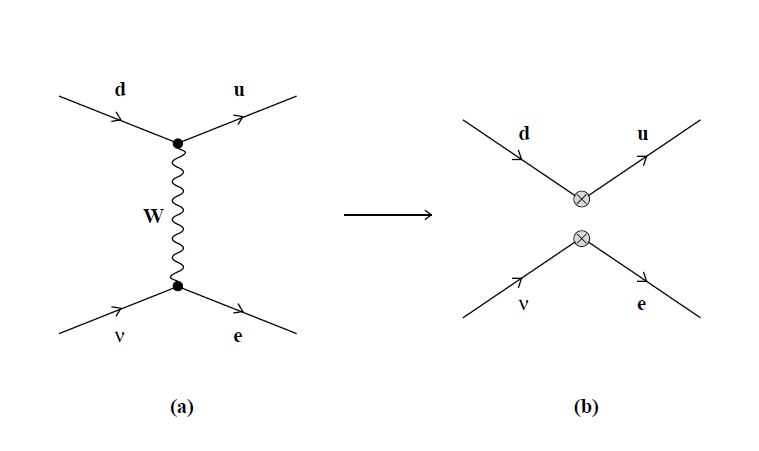
\includegraphics[width=12cm]{fermi_int.JPG}
\caption{\label{fig:fermi_int}
Underlying quark process of $\beta$ decay. (a) represent the SM description and (b) represent the effective representation \cite{Buras:1999rb} .}
\end{figure}
In general, the phenomenology of any weak hadronic decay is given by the following effective Hamiltonian.
\begin{eqnarray}\label{eff_hamiltonian}
\mathcal{H}_{e f f}=\frac{G_{F}}{\sqrt{2}} \sum_{i} V_{\mathrm{CKM}}^{i} C_{i}(\mu) Q_{i}(\mu).
\end{eqnarray}
Here $Q_i$ are relavent local operators that govern the particular decay, $C_{i}(\mu)$ are the Wilson coefficients, which describe the strength of a given operator that enters the Hamiltonian and $V_{\mathrm{CKM}}^{i}$ is the relevent CKM matrix element to the decay. Simply, the equation (\ref{eff_hamiltonian}) can be thought of as a series of vertices multiplied by effective coupling constants $C_i$ \cite{Buras:1999rb}. This effective series is known as an operator product expansion (OPE) \cite{Wilson:1969zs, Wilson:1972ee,Zimmermann:1972tv}. The local operators (vertices) in the OPE involved with the strong and weak interactions, and they can be classified with respect to the Dirac structure, color structure and the type of quarks and leptons relevant for the decay.
\subsection{OPE for B meson decays}\label{section:OPE_b}
The $B$ meson is a bound state of a $b$ quark and a parton (light quark). The decay of $B$ is governed by the processes that involve $W, Z$ and $t$ quark, and they represent the physics at short distance (high energy) scales $\mathcal{O}(M_{W,Z}, m_t)$. At the long distance (energy$\sim \Lambda_{\text{QCD}}$) scale, the hadronization process govern the decay since $\alpha_s(\Lambda_{\text{QCD}})\sim \mathcal{O}(1)$, where at $\Lambda_{\text{QCD}}$ the nonperturbative effects become prominent. The hadronic decay at $\mathcal{O}(m_b)$ is given by effective point like vertices, which are represented by local operators $Q_i$. The Wilson coefficients can be thought of as the coupling constants associated with these $Q_i$.\par 
For instance, the non-leptonic $B$ meson decays involve the following set of local operators.
\begin{eqnarray}
\begin{array}{l}{\text { Current-Current: }} \\ {\qquad Q_{1}=\left(\bar{c}_{\alpha} b_{\beta}\right)_{V-A}\left(\bar{s}_{\beta} c_{\alpha}\right)_{V-A} \quad Q_{2}=(\bar{c} b)_{V-A}(\bar{s} c)_{V-A}}\end{array}
\end{eqnarray}
\begin{eqnarray}
\begin{array}{l}{\text { QCD-Penguins : }} \\ {\qquad Q_{3}=(\bar{s} b)_{V-A} \sum_{q=u, d, s, c, b}(\bar{q} q)_{V-A} \quad Q_{4}=\left(\bar{s}_{\alpha} b_{\beta}\right)_{V-A} \sum_{q=u, d, s, c, b}\left(\bar{q}_{\beta} q_{\alpha}\right)_{V-A}}\\{\qquad Q_{5}=(\bar{s} b)_{V-A} \sum_{q=u, d_{s}, c, b}(\bar{q} q)_{V+A} \quad Q_{6}=\left(\overline{s_{\alpha}} b_{\beta}\right)_{V-A} \sum_{ q=u, d_{s}, c, b}\left(\bar{q}_{\beta} q_{\alpha}\right)_{V+A}}\end{array}
\end{eqnarray}
\begin{eqnarray}
\begin{array}{l}{\text { Electroweak-Penguins : }} \\ {Q_{7}=\frac{3}{2}(\bar{s} b)_{V-A} \sum_{q=u, d, s, c, b} e_{q}(\bar{q} q)_{V+A} \quad Q_{8}=\frac{3}{2}\left(\bar{s}_{\alpha} b_{\beta}\right)_{V-A} \sum_{q=u, d, s, c, b} e_{q}\left(\bar{q}_{\beta} q_{\alpha}\right)_{V+A}} \\ {Q_{9}=\frac{3}{2}(\bar{s} b)_{V-A} \sum_{q=u, d, s, c, b} e_{q}(\bar{q} q)_{V-A} \quad Q_{10}=\frac{3}{2}\left(\bar{s}_{\alpha} b_{\beta}\right)_{V-A} \sum_{q=u, d, s, c, b} e_{q}\left(\bar{q}_{\beta} q_{\alpha}\right)_{V-A}}\end{array},
\end{eqnarray}
where $\alpha$ and $\beta$ are corresponding color indices, $e_q$ is the electric charge of quarks. The operators $Q_2, Q_{3-6}$ and $Q_7, Q_9$ are generated due to the tree level $W^{\pm}$ exchange, gluon penguin and $\gamma, Z^0$ penguin diagrams respectively.
The Wilson coefficients provide the contribution of the short distant ( energy scale higher than $\mu$ ) physics.  Since QCD is asymptotically free, these Wilson coefficients can be  perturbatively calculated. The $C_i$ include the contributions from the $t$ quark, $W$, $Z$, Higgs and SM extensions. In general, Wilson coefficients depend on $m_t$ and the masses of new particles from SM extensions.\par
The scale $\mu$ separates the physics contribution to the decay amplitude to long distance and short distance. Short distance physics governs the interaction at energies that are higher than the value of $\mu$. Whereas, long distance physics governs the interaction at the energies lower than the value of $\mu$. In practice $\mu$ is chosen at the order of $m_b$ (mass of the decaying hadron). Since $\mu = \mathcal{O}(m_b)\gg \Lambda_{\text{QCD}}$, the $C_i$ can be calculated perturbatively in $B$ decays.\par
Long distance physics are contained in local matrix elements $\langle Q_i(\mu)\rangle$. Using the \textit{renormalization group equation} (RGE) we evolve the scale from $\mu=\mathcal{O}(M_W)$ down to $\mathcal{O}(m_b)$. The full amplitude is independent of $\mu$, and it implies the cancellation of the $\mu$ dependence in $C_i$ with the $\mu$ dependence of $\langle Q_i(\mu)\rangle$.
\vspace{-0.4cm}
\subsubsection{Inclusive and exclusive $B$ decays}
\vspace{-0.3cm}
\textit{Exclusive} decays imply the measurement of energy and momenta of all the final state particles. Whereas, in \textit{inclusive} decays the probability of particle decay into a sum of final states ($X$) with a given set of global quantum numbers such as energy and momentum is measured.\par
The amplitude for exclusive decays such as $B$ decay in to final states $F=\pi \nu \bar{\nu}, \pi \pi, D K$ is given by 
\begin{eqnarray}\label{BtoFex}
A(M \rightarrow F)=\left\langle F\left|\mathcal{H}_{e f f}\right| B\right\rangle=\frac{G_{F}}{\sqrt{2}} \sum_{i} V_{C K M}^{i} C_{i}(\mu)\left\langle F\left|Q_{i}(\mu)\right| B\right\rangle
\end{eqnarray} 
where $\left\langle F\left|Q_{i}(\mu)\right| B\right\rangle$ are the hadronic matrix elements of operators $Q_i$ between the initial $B$ meson state and the final state $F$. Evaluation of this matrix element is necessary for the calculation of the exclusive amplitude. The Wilson coefficients $C_i(\mu)$ in equation (\ref{BtoFex}) depends on both the scale $\mu$ and the renormalization scheme that was used for local operators. This is calculated in the renormalization group improved perturbation theory. The hadronic matrix elements $\langle Q_i\rangle$ also depend on both $\mu$ and the renormalization scheme. \par
The evaluation of $\langle Q_i(\mu)\rangle$ requires nonperturbative methods such as lattice calculations, the $1/N_c$ expansion ($N_c$ is the number of colors), QCD sum rules, hadronic sum rules, chiral perturbation theory and so on. Also, for some $B$ meson decays these matrix elements can be analyzed using the \textit{heavy quark effective theory} (HQET).\par
The amplitude for an inclusive $B$ decay is given by
\begin{eqnarray}\label{BtoXinc}
A(B \rightarrow X)=\frac{G_{F}}{\sqrt{2}} \sum_{f \in X} V_{\mathrm{CKM}}^{i} C_{i}(\mu)\left\langle f\left|Q_{i}(\mu)\right| B\right\rangle
\end{eqnarray} 
Unlike the exclusive decays, the scheme dependence in inclusive decay matrix elements can be effectively evaluated. Because of this, the cancellation of this scheme dependence with the scheme dependence in $C_i$ can be systematically studied \cite{Neubert:1993ch}. Therefore, studying the inclusive $B$ meson decays become important from the practitioner's point of view.\par
Inclusive decays have two main advantages over exclusive decays. 
\begin{itemize}
\item The bound state related effects such as Fermi motion \cite{Neubert:1993ch} of heavy quark inside the hadron can be systematically described by heavy quark expansion
\item The bound state effects related to the final state hadrons are removed due to the consideration of final state as a sum of hadronic channels. 
\end{itemize}
The second feature is realized due to the application of \textit{quark hadron duality}\cite{Poggio:1975af, Shifman:2000jv}. This suggests that at high energy scales ($\mu$) the cross section of hadronic decays, which are averaged over the energy range, can be approximately given by the cross sections that are evaluated by quark and gluon pertrurbation theory. 

\section{Heavy quark effective theory (HQET)}\label{sec:HQET}
\subsection{Heavy quark symmetry}\label{sec:heavy_quark_sym}
Due to asymptotic freedom \cite{Gross:1973id} at large momentum transfer (short distance scale), the effective coupling constants $C_i$ become small. Whereas at low energy transfer (long-distance scale), the coupling becomes strong, and the process becomes nonperturbative. This property of QCD makes studying the processes that include decay of heavy quarks easier than the processes that include only the light quarks. These nonperturbative phenomena are dominated at the scale $R_{\text{had}}\sim 1/\Lambda_{\text{QCD}}\sim 1\text{ fm}$ \cite{Neubert:1997gu}. This scale also determines the size of the hadrons. When a mass of a quark ($M_Q$) is much larger than the $\Lambda_{\text{QCD}}$ ($M_Q\gg\Lambda_{\text{QCD}}$), then we call it a heavy quark. In the SM $c,\,b$ and $t$ quarks are considered as heavy.\par
The system of heavy quark and light quarks is a bound state, which is complicated to analyze. The typical momentum exchange between these heavy and light constituents are of $\mathcal{O}(\Lambda_{\text{QCD}})$. This bound state of heavy quark and light quarks can be thought of as heavy quark sitting at the center of the strongly interacting cloud of  \textit{partons} (light quarks). The corresponding Compton wavelength ($\lambda_Q$) for a heavy quark is much less than the size of hadron $\lambda_Q\ll R_{\text{had}}$. This means the heavy quark's quantum numbers are resolved at very small distances compared to $R_{\text{had}}$. In contrast, the soft gluons exchanged between the heavy quark and the light quarks are resolved at much larger distances than the heavy quark. Due to this, the light degrees of freedom become blind to the flavor and spin orientation of the heavy quark. These light quarks will only feel the color field generated by the heavy quark, and it is extended over a larger area compared to the scale of the heavy quark. As shown above, this nature of the interactions between heavy quark and the partons provide a clear separation of scales, which makes this bound state a suitable candidate for an EFT analysis.\par 
Since the heavy quark is irrelevant for the effective analysis, we use the limit $M_Q\rightarrow \infty$ in deriving the theory. Also, in this limit, the differences between various hadronic states that have different heavy flavors tend to have the same configuration. In fact, the configuration of these different hadronic states is determined by the configuration of the light quarks. This property provides the relation between the heavy meson states such as $B, D, B^{*} \text { and } D^{*}$ or between the heavy baryon states such as $\Lambda_b$ and $\Lambda_c$. This means if we change the heavy quark with velocity $v$ in the system with another heavy quark with the same four-velocity and different flavor or spin, the configuration of the light quarks remains the same. Both heavy quarks will remain as static \textit{color sources}. Therefore, we obtain a new symmetry in the effective theory, which includes $N_h$ number of heavy quarks. This symmetry is known as \textit{heavy quark symmetry}, and it is $SU(2N_h)$ internal continuous symmetry \cite{Neubert:1997gu}.  

\subsection{Constructing the HQET Lagrangian}\label{sec:HQET_Lag_constr}
Since the presence of the heavy quark is irrelevant for the configuration of light quarks, at low energies, we can construct a low energy theory in which the heavy degrees of freedom does not appear. This is known as the \textit{``integrating out"}.
This integrating out procedure is similar to the above discussed \textit{Fermi theory} of weak interactions. \par
The \textit{heavy quark effective theory} (HQET) is constructed to simplify the complicated interaction between the heavy quark and the partons by the exchange of soft gluons \cite{Eichten:1980mw, Isgur:1989vq, Balzereit:1996yy, Grinstein:1990mj}. The heavy quark masses $M_Q$ is the high energy scale of the theory. Whereas, we construct the theory to study the interactions at the scale of $\Lambda_{\text{QCD}}$.
 As shown in the section \ref{section:OPE_b}, scale $\mu$ separates long distance and short distance physics contributions. The short distance physics are obtained at the energy scales larger than the heavy quark mass. By considering these two limits for the scale $\mu$, we introduce the scale as in the range $\Lambda_{\text{QCD}}\ll\mu \ll M_Q$ \cite{Neubert:1997gu}. \par
Since we assume the heavy quark is static inside the heavy hadron's rest frame, heavy quark's velocity is equal to the hadron's velocity $v$. Therefore, the momentum of the heavy quark inside the bound state is given by
\begin{eqnarray}
p_{Q}^{\mu}=M_{Q} v^{\mu}+k^{\mu},
\end{eqnarray} 
where $v$ is the four-velocity of the heavy meson, and it is given by $v=(1,0,0,0)$. The $v\cdot v=1$ and $k$ is the residual momentum. The $k$ determines the off-shellness of heavy quarks due to the interactions with light partons. This provides $k\sim\Lambda_{\rm{QCD}}\ll M_Q v$. The changes to the heavy quark velocity $v$ due to these soft interactions are small, and they vanish as $\Lambda_{\mathrm{QCD}} / m_{Q} \rightarrow 0$. \par
As shown in \cite{Neubert:2005mu, Petrov:2016azi}  the near on shell Dirac spinor has two large and two small components, using this, the quantum field for the heavy quark can be defined as follows:
\begin{equation}\label{eqn:HQET_param}
Q(x)= e^{-iM_{Q}\upsilon \cdot x}[h_{\upsilon}(x)+H_{\upsilon}(x)].
\end{equation}
Where $h_{\upsilon}(x)=e^{iM_{Q}\upsilon\cdot x}\dfrac{(1+\slashed{\upsilon})}{2}Q(x)$ represents the large ``upper" component and $H_{\upsilon}(x)=e^{iM_{Q}\upsilon.x}\dfrac{(1-\slashed{\upsilon})}{2}Q(x)$ represents the small ``lower" components. These large and small component fields satisfy $\slashed{v} h_{v}=h_{v} \text { and } \slashed{v} H_{v}=-H_v$. Now the full QCD Lagrangian
\begin{eqnarray}
\mathcal{L}_{Q}=\bar{Q}\left(i \slashed{ D}-m_{Q}\right) Q
\end{eqnarray} 
can be re written as follows:
\begin{eqnarray}\label{eqn:HQET_Lag1}
\mathcal{L}_{Q}=\bar{h}_{v} i v \cdot D h_{v}-\bar{H}_{v}\left(i v \cdot D+2 m_{Q}\right) H_{v}+\bar{h}_{v} i \slashed{D}_{\perp} H_{v}+\bar{H}_{v} i \slashed{D}_{\perp} h_{v},
\end{eqnarray}
where $D_{\perp}^{\mu}=D^{\mu}-v^{\mu} v \cdot D$ is the orthogonal component of the covariant derivative to the heavy quark velocity ($v \cdot D_{\perp}=0$). In the rest frame of the heavy quark $D_{\perp}$ only contains the spatial components of the covariant derivative ($D_{\perp}=(0, \vec{D})$).
From equation (\ref{eqn:HQET_Lag1}), we find that $h_{v}$ describes massless degree of freedom. Whereas, the $H_{v}$ describes a heavy degree of freedom with mass $2M_Q$. The third and fourth terms in the equation (\ref{eqn:HQET_Lag1}) describe pair creation and anhilation of heavy quark and heavy anti-quark. These heavy degrees of freedom can be eliminated using the equation of motion. The HQET equation of motion provides
\begin{eqnarray}\label{eqn:HQET_EOM}
\left(i v \cdot D+2 M_{Q}\right) H_{v}=i \slashed{ D}_{\perp} h_{v}
\end{eqnarray}
by solving the equation (\ref{eqn:HQET_EOM}) for $H_{v}$ 
\begin{eqnarray}\label{eqn:HQET_EOM1}
H_{v}=\frac{1}{2 M_{Q}+i v \cdot D} i \slashed{ D}_{\perp} h_{v}
\end{eqnarray} 
This eliminate the small component of the heavy quark field in the equation (\ref{eqn:HQET_Lag1}).
\begin{eqnarray}\label{eqn:HQET_Lag_1}
\mathcal{L}_{\mathrm{eff}}=\bar{h}_{v} i v \cdot D h_{v}+\bar{h}_{v} i \slashed{ D}_{\perp} \frac{1}{2 M_{Q}+i v \cdot D} i \slashed{ D}_{\perp} h_{v}
\end{eqnarray} 
In momentum space the derivatives that are acting on $h_v$ produce powers of residual momentum $k$. Because of $k\ll M_{Q}v$, we expand the equation (\ref{eqn:HQET_EOM1}) in a \textit{Taylor series}. Applying this expansion in equation (\ref{eqn:HQET_Lag_1}):
\begin{eqnarray}
\mathcal{L}_{\mathrm{eff}}=\bar{h}_{v}i v . D h_{v}+\bar{h}_{v}\frac{i \slashed{ D}_{\perp}}{2 M_{Q}}\left(1+\sum_{n=0}^{\infty}\left(-\frac{i v \cdot D}{2 M_{Q}}\right)^{n}\right) i \slashed{ D}_{\perp} h_{v}
\end{eqnarray}
For $n=0$ the above expression can be further simplified using the following identity
\begin{eqnarray}
\slashed{D}_{\perp} \slashed{ D}_{\perp}=g_{\mu \nu} D_{\perp}^{\mu} D_{\perp}^{\nu}-i \sigma_{\mu \nu} D_{\perp}^{\mu} D_{\perp}^{\nu}
\end{eqnarray}
where $\sigma_{\mu \nu}=\frac{i}{2}\left[\gamma_{\mu}, \gamma_{\nu}\right]$.
Following from this the resulting Lagrangian is obtained as an expansion in $1/M_{Q}^{n}$.
\begin{eqnarray}\label{Hlag}
{\cal L}_{\rm eff}=\bar{h}_{\upsilon}\left(i\upsilon \cdot D-\dfrac{D^{2}}{2M_{Q}}-\dfrac{g}{4M_{Q}}\sigma_{\mu\nu}G^{\mu\nu}\right)h_{\upsilon}+O\left(\dfrac{1}{M_{Q}^{2}}\right),
\end{eqnarray}
where, $G^{\mu\nu}$ is Chromo-electromagnetic field strength tensor.\par
 In the limit $M_Q\rightarrow \infty$ only the first term in equation (\ref{Hlag}) remains
\begin{eqnarray}\label{eqn:HQET_Lag_Infty}
\mathcal{L}_{\infty}=\bar{h}_{v} i v \cdot D h_{v}.
\end{eqnarray} 
\subsubsection{Operators at order $\mathcal{O}(1/M_Q)$ in the HQET Lagrangian}\label{sec:order_1/M_Q }
\vspace{-0.3cm}
Consider the second and the third terms in equation (\ref{Hlag}). The operator, 
\begin{eqnarray}
\mathcal{O}_{\mathrm{kin}}=\frac{1}{2 M_{Q}} \bar{h}_{v}\left(i D_{\perp}\right)^{2} h_{v} \rightarrow-\frac{1}{2 M_{Q}} \bar{h}_{v}(i \vec{D})^{2} h_{v},
\end{eqnarray}
is the kinematic energy of the heavy quark's residual motion. The operator, $\mathcal{O}_{\mathrm{mag}}$ defined in equation (\ref{eqn:mag_op}) is the color-magnetic coupling between heavy quark spin and gluon field.
\begin{eqnarray}\label{eqn:mag_op}
\mathcal{O}_{\mathrm{mag}}=\frac{g_{s}}{4 M_{Q}} \bar{h}_{v} \sigma_{\mu \nu} G^{\mu \nu} h_{v} \rightarrow-\frac{g_{s}}{M_{Q}} \bar{h}_{v} \vec{S} \cdot \vec{B}_{c} h_{v},
\end{eqnarray}
where $\vec{S}$ are the Pauli spin matrix elements, and $B_{c}^{i}=-\frac{1}{2} \epsilon^{i j k} G^{j k}$, which are the components of color magnetic field. \cite{Pauli:1941zz, Dittrich:1985yb, Lee:2006nc}.\par

\section{Non-relativistic QCD}\label{NRQCD}
HQET describes systems that include a single heavy quark and light partons. In HQET the heavy quark's kinetic energy is considered as a power correction. When considering multiple heavy quarks the strong interaction between them at short distances is determined by a single gluon exchange \cite{Manohar:2000dt}. This gluon exchange is defined by a Coulomb potential, and for $\bar{Q}Q$ in a color single state this potential is an attractive potential. This attractive potential is then compensated by heavy quark kinetic energy. This makes the kinetic energy of the heavy quark field play an important role in stabilizing the heavy mesons. The heavy quark kinetic energy cannot be treated as a power correction. Thus, we use a different power counting scheme in NRQCD compared to HQET. This difference is further illustrated in the following example.\par
Consider the figure \ref{fig:Box_diag_two_glu_ex}, which represents a box diagram with two heavy quarks exchange gauge particles (gluons or photons).
\begin{figure}[H]
\centering
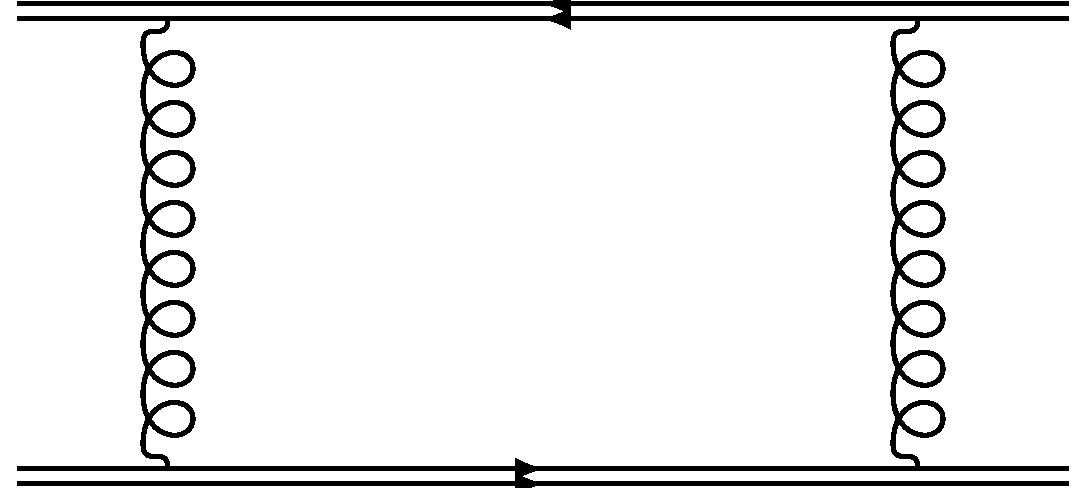
\includegraphics[width=8cm]{box diagram with two heavy quarks1.pdf}
\caption{\label{fig:Box_diag_two_glu_ex}
Box diagram for two heavy quark exchanging gauge particles}
\end{figure}
The integral $I$ that corresponds to the figure \ref{fig:Box_diag_two_glu_ex} is given by \cite{Petrov:2016azi}

\begin{eqnarray}\label{eqn:box_diag_int}
I \sim \int \frac{d^{d} q}{(2 \pi)^{d}} \frac{1}{q^{0}+i \epsilon} \frac{1}{-q^{0}+i \epsilon} \frac{1}{(q+k)^{2}+i \epsilon} \frac{1}{(q-k)^{2}+i \epsilon}
\end{eqnarray}

In the equation (\ref{eqn:box_diag_int}), we find two poles at $q^0=\pm i \epsilon$. These poles are coming from the heavy quark propagators, and they cause a ``pinch singularity". As a result, we cannot deform the contour of the integration without crossing one of these poles \cite{Petrov:2016azi}. To overcome this singularity we need to introduce a new power counting scheme. In this new power counting scheme the importance of the heavy quark kinetic energy is pronounced.\par
In NRQCD the quarkonium is described by an effective Lagrangian, which is expanded as a power series in $v/c$, where $c$ is the vacuum speed of light. The NRQCD Lagrangian can be obtained by using the $c\rightarrow \infty$ limit in the full QCD Lagrangian. 
\subsection{NRQCD Lagrangian}
As shown above, the difference between the HQET and NRQCD is manifested in the first two terms of the effective Lagrangian.
\begin{eqnarray}
\mathcal{L}=Q^{\dagger}(iD^{0})Q+Q^{\dagger}\frac{\bm{D}^2}{2m}Q.
\end{eqnarray} 
In HQET the first term is of $\mathcal{O}(\Lambda_{\rm{QCD}})$ and second term is considered as a correction term of $\mathcal{O}(\Lambda^{2}_{\rm{QCD}}/m)$. Whereas, in NRQCD both terms are of $\mathcal{O}(mv^2)$. Because of this, the heavy quark propagator in both effective theories have different forms. For instance, the heavy quark propagator in HQET is given by $i /\left(k^{0}+i \epsilon\right)$. The NRQCD heavy quark propagator is given by
\begin{eqnarray}\label{eqn:NRQCD_propagator}
\frac{i}{\left(k^{0}-\mathbf{k}^{2} / 2 m+i \epsilon\right)}
\end{eqnarray}
This full NRQCD propagator causes problems in matching calculations. As shown above, the HQET propagator is $m_Q$ independent. Because of this we count the powers of $1/m_Q$ directly from the vertex factors.  For instance, if $s<r$ the effective vertex of $\mathcal{O}(1/m_Q^r)$ does not provide any contribution to terms of $\mathcal{O}(1/m_Q^s)$. Then the matching in HQET is done by expanding Greens function to the desired order in $1/m_Q$. But the NRQCD propagator contains additional power suppressed factors. These factors can wreck the simple power counting of Greens function \cite{Petrov:2016azi}. The solution for this problem is provided in  \cite{Manohar:1997qy}.\par
In \cite{Manohar:1997qy} the full NRQCD propagator is expanded, and the extra terms were treated as a perturbation. The expansion of full NRQCD propagator is given by
\begin{eqnarray}
\frac{1}{k^{0}-\mathbf{k}^{2} / 2 m+i \epsilon}=\frac{1}{k^{0}}+\frac{\mathbf{k}^{2}}{2 m\left(k^{0}\right)^{2}}+\cdots
\end{eqnarray}
The series expansion of propagator prevents the appearance of positive powers of the mass terms. Whereas, the full NRQCD propagator provides these positive powers. Thus, by expanding the NRQCD propagator the NRQCD and HQET matching conditions can be computed using the same procedure.\par
The NRQCD Lagrangian upto dimension seven ($\mathcal{O}(1/m^3)$) is provided in equation (\ref{eqn:NRQCD_Lag_dim_7}). 
This Lagrangian is computed to one loop, and it only considers the terms that are bilinear in fermions \cite{Manohar:1997qy}. In equation (\ref{eqn:Dim_8_Lagrangian}) we provide the dimension eight Lagrangian. This is first obtained in our work \cite{Gunawardana:2017zix}.
 
\section{Applications}
\subsection{Heavy quark spectroscopy}
As shown in the section \ref{sec:heavy_quark_sym}, the dynamics of hadronic bound state with one heavy quark does not depend on its heavy quark's flavor or spin. Because of this, states with different heavy quark flavors can be related to each other. The hadronic states, therefore, are classified by  the quantum numbers of the light degrees of freedom \cite{Falk:1991nq}. From the spin symmetry we find that the total spin of these partons are doubly degenerated with total spin $J=j \pm \frac{1}{2}$ \cite{Isgur:1991wq}.\par
The mass of a hadron $H_Q$ is related to it's heavy quark as follows:
\begin{eqnarray}\label{eqn:quark_hadron_mass_relation}
M_{H_{Q}}=M_{Q}+\bar{\Lambda}+\frac{\Delta M^{2}}{2 M_{Q}}+O\left(1 / M_{Q}^{2}\right), 
\end{eqnarray}
where $\bar{\Lambda}= M_{H_Q}-M_Q$ and $\Delta M^2$ is originated from the order $1/M_Q$ terms in effective Lagrangian. In particular, the mass splitting ($\Delta M^2$) for heavy hadrons are defined as
\begin{eqnarray}\label{eqn:mass_split}
\Delta M^{2}=-\lambda_{1}+2\left[J(J+1)-\frac{3}{2}\right] \lambda_{2},
\end{eqnarray} 
where $\lambda_1$ and $\lambda_2$ are nonperturbative parameters, which parametrize the kinetic energy and the chromo-magnetic interaction of heavy quark in heavy hadron. For instance, consider the $B$ and $B^*$ mesons. These hadronic states are the members of spin doublet $j=\frac{1}{2}$, and they are ground-sate pseudo scalar ($J=0$) and vector ($J=1$) states respectively. Using the equations (\ref{eqn:quark_hadron_mass_relation}) and (\ref{eqn:mass_split}) we obtain
\begin{eqnarray}
M_B&=& M_b+\bar{\Lambda}-\frac{\lambda_1}{2M_b}-\frac{3\lambda_2}{2M_b}\nonumber\\
M_B^*&=& M_b+\bar{\Lambda}-\frac{\lambda_1}{2M_b}+\frac{\lambda_2}{2M_b}
\end{eqnarray}
 Therefore, the mass splitting between these states is given by
\begin{eqnarray}\label{eqn:mass_split_expression}
\begin{aligned} M_{B^{*}}^{2}-M_{B}^{2} &=4 \lambda_{2}+O\left(1 / M_{b}\right) \end{aligned}
\end{eqnarray} 
PDG average for the $B$ and $B^*$ mass spliting is
\begin{eqnarray}
M_{B^{*}}^{2}-M_{B}^{2} = 0.478\pm 0.003 \text{ GeV}^{2}
\end{eqnarray}
From this we obtain 
\begin{eqnarray}  
\lambda_{2} = 0.119\pm 0.001 \text{ GeV}^{2}
\end{eqnarray}
These results are obtained by assuming the $m_b\rightarrow \infty$ limit.\par
The nonperturbative parameter $\lambda_1$ contains the information about ``smearing" in heavy quark momentum \cite{Ball:1993xv}. This parameter is defined as
\begin{eqnarray}
2\lambda_1=-\langle H_Q|\bar{h}_v D^2_{\perp}h_v|H_Q\rangle.
\end{eqnarray}
The $\lambda_1$ can be calculated using the QCD sum rule approch \cite{Ball:1993xv}.Theoretical estimate for the $\lambda_1$ is given in \cite{Gambino:2016jkc}. 
	\chapter{Background :  The $\bar{B}\rightarrow X_s\gamma$ decay}
The inclusive radiative $\bar{B}\rightarrow X_s\gamma$ decay is an important new physics probe. Since this is a FCNC process, it does not occur at tree level in the SM. Therefore, it can be highly sensitive to new physics. In particular, these new physics sources can modify the Wilson coefficient $C_{7\gamma}$, and they may introduce new weak phases that can enhance the SM CP asymmetry.\par
The $b\rightarrow s\gamma$ is the underlying partonic decay of the inclusive $B\rightarrow X_s\gamma$ decay. This $b$ to $s$ transition is one of the most reliably calculable FCNC processes in SM \cite{Ritchie:2013xc}. The final states $X_s$ represent a final state that contains a $s$ quark\par
The current SM next to-next to leading (NNLO) prediction for the $\bar{B}\rightarrow X_s\gamma$ branching ration is $\mathcal{B}^{\rm{SM}}_{X_s\gamma}=(3.36\pm0.23)\times 10^{-4}$ \cite{Misiak:2015xwa, Czakon:2015exa}. The experimental world average is $\mathcal{B}^{\rm{exp}}_{X_s\gamma}= (3.32\pm0.15)\times 10^{-4}$ \cite{Amhis:2019ckw, Chen:2001fja, Aubert:2007my, Lees:2012wg, Lees:2012ym, Saito:2014das, Belle:2016ufb}. The experimental uncertainty on the branching ratio is expected to reduce from $\pm 4.5\%$ to around $\pm 2.6\%$ in future thanks to Belle II measurements \cite{Kou:2018nap}. With these new precision measurements, SM prediction can strongly constrain the BSM. Therefore, improving the precision of the theoretical prediction is important.\par

The uncertainty of the SM prediction  arise from several sources. These uncertainties were combined in quadrature to obtain the total uncertainty ($\pm 6.8\%$). The breakdown of these uncertainties is as follows:
The nonperturbative contribution to the uncertainty is $\pm 5\%$ \cite{Benzke:2010js}, parametric uncertainty is $\pm 2\%$, perturbative uncertainty is $\pm 3\%$, the uncertainty from interpolating the charm mass in two-loop is $\pm 3\%$ \cite{Czakon:2015exa}.\par

Since the nonperturbative uncertainty provides the largest contribution to the total uncertainty, we would like to explore the possibility of improving this estimate. The question that we are prompt to ask is ``how do we reduce this uncertainty?''. In the following work, we address the issue of reducing the nonperturbative contribution of the theoretical prediction.

\section{The inclusive decay rate}
The inclusive decay rate for the $\bar{B}\rightarrow X_s\gamma$ is obtained by using the optical theorem. This theorem relates the decay rate to the imaginary part of the forward scattering amplitude. The $\bar{B}\rightarrow X_s \gamma$ decay is can be written as
\begin{eqnarray}\label{eqn:Inclsv_dacay_rate_btoxgamm}
\Gamma\left(\bar{B} \rightarrow X_s\gamma\right)=\frac{1}{M_{B}} \operatorname{Im}\left\langle \bar{B}|\mathbf{T}| \bar{B}\right\rangle,
\end{eqnarray} 
where $\mathbf{T}$ is related to the effective Lagrangian. However, instead of effective Lagrangian we use the effective Hamiltonian ($\mathcal{H}_{\mathrm{eff}}$)
\begin{eqnarray}\label{eqn:Trans_matrix_btoxgam}
\mathbf{T}=i \int \mathrm{d}^{4} x T\left\{\mathcal{H}_{\mathrm{eff}}(x), \mathcal{H}_{\mathrm{eff}}(0)\right\}, 
\end{eqnarray}
where $\mathcal{H}_{\mathrm{eff}}$ is obtained after integrating out the $W$ boson \cite{Benzke:2010js}. The effective Hamiltonian is given by

\begin{equation}\label{eq:Weak Hamiltonian}
   {\cal H}_{\rm eff} = \frac{G_F}{\sqrt{2}} \sum_{q=u,c} \lambda_q\,
   \bigg( C_1\,Q_1^q + C_2\,Q_2^q + \sum_{i=3,...,6} C_i\,Q_i 
   + C_{7\gamma}\,Q_{7\gamma} + C_{8g}\,Q_{8g} \bigg) \,,
\end{equation}
where $\lambda_q=V_{qb} V_{qs}^*$, $C_{i}$ are the Wilson coefficients and $Q_i$ are the effective operators.
This Hamiltonian describes the underlying are weak interaction in the decay process.\par
The decay rate and the photon spectrum related to the restricted discontinuity of forward scattering matrix element \cite{Benzke:2010js}.
\begin{eqnarray}\label{eqn:discont_eval}
d \Gamma\left(\bar{B} \rightarrow X_{s} \gamma\right) \propto \operatorname{Disc}_{\mathrm{restr}}\left[i \int d^{4} x\left\langle\bar{B}\left|\mathcal{H}_{\mathrm{eff}}^{\dagger}(x) \mathcal{H}_{\mathrm{eff}}(0)\right| \bar{B}\right\rangle\right],
\end{eqnarray}
where the restricted discontinuity implies that the discontinuity is restricted by the requirement that the cut must be applied on photon and strange quark propagators. 
\subsection{Kinematics of the decay} 
In its rest frame, the $B$ meson is decaying into a hadronic jet, which carries a momentum $P_X$, and to a photon, which carries a momentum $q$. The momentum of the heavy hadron is $M_{B} v=P_{X}+q$, where $v$ is the four velocity of the $B$ meson. In the $B$ meson rest frame $v=(1,0,0,0)$. We can align $\vec{q}$ in the negative $z$ direction and define two light-like vectors $n^{\mu}=(1,0,0,1)$ and $\bar{n}^{\mu}=(1,0,0,-1)$. These $n$ and $\bar{n}$ vectors satisfy $\bar{n}+n=2v$, $\bar{n}\cdot n=2$ and $n\cdot v=\bar{n}\cdot n=1$ \cite{Paz:2009ut}. In general, any four vector can be decomposed as 
\begin{eqnarray}\label{eqn:4vec_decomp}
a^{\mu}=\bar{n} \cdot a \frac{n^{\mu}}{2}+n \cdot a \frac{\bar{n}^{\mu}}{2}+a_{\perp}^{\mu}.
\end{eqnarray}
For the choice of $v,n,\bar{n}$ the transverse component ($\perp$) is spanned by $(0,1,0,0)$ and $(0,0,1,0)$. These transverse indices can be contracted using
\begin{eqnarray}\label{eqn:Transverse_indices_contract}
g_{\perp}^{\mu \nu}=g^{\mu \nu}-\frac{n^{\mu} \bar{n}^{\nu}+n^{\nu} \bar{n}^{\mu}}{2}, \quad \epsilon_{\perp}^{\mu \nu}=\frac{1}{2} \epsilon^{\mu \nu \alpha \beta} \bar{n}_{\alpha} n_{\beta}
\end{eqnarray}
where we use the following convention for the levi-civita tensor $\epsilon_{0123}=1$.\par
The conservation of four momentum provides that there is only one independent kinematical variable in $\bar{B}\rightarrow X_s\gamma$ decay that is the photon energy $E_{\gamma}$.

\subsection{Factorization}
At the leading order the $\bar{B}\rightarrow X_s\gamma$ decay can be thought of as a decay of constituent $b$ quark decaying into an $s$ quark and a photon. This constituent quark decay is expressed by the electromagnetic dipole operator $Q_{7\gamma}$
\begin{eqnarray}
Q_{7\gamma} &= \frac{-e m_b}{8\pi^2}\bar s\sigma_{\mu\nu}(1+\gamma_5)F^{\mu\nu}b.
\end{eqnarray}
However, this is not the only way to produce a photon. For instance, a gluon or a quark pair that was produced at the weak vertex can be converted to a photon, and these processes are described by the operators $Q_{8 g}=\left(-g / 8 \pi^{2}\right) m_{b} \overline{s} \sigma_{\mu \nu} G^{\mu \nu}\left(1+\gamma_{5}\right) b$ and $Q_{1}^{c}=(\overline{c} b)_{V-A}(\overline{s} c)_{V-A}$ respectively. The effective Hamiltonian for $\bar{B}\rightarrow X_{s}\gamma$ needs to account for all of these operators to accutrately describe the decay process.\par
The major contribution to the effective Hamiltonian arises from the operators $Q_{1}^{q}, Q_{7\gamma}$ and $Q_{8g}$ \cite{Benzke:2010js}. This is because the Wilson coefficients of these operators are relatively larger than the rest.\par
At the leading order the only the operator pair $Q_{7\gamma}-Q_{7\gamma}$ contributes to the decay rate. The contributions from operators such as $Q_1^q$ and $Q_{8g}$ give higher order contributions, and they either ``cost" a factor of $\alpha_s$ or $1/m_{b}$ in the decay rate calculation.\par
The shape of the $\bar{B}\rightarrow X_s\gamma$ photon spectrum probes the nonperturbative hadronic physics in the decay. At the leading order this photon spectrum is related to a universal shape function that parametrizes the $b$ quark momentum in the $B$ meson bound state. This shape function also parameterizes the leading order bound state effects of semileptonic decay $\bar{B}\rightarrow X_u l \nu$. However, the contributions of operators other than $Q_{7\gamma}-Q_{7\gamma}$ to  $\bar{B}\rightarrow X_s\gamma$ make the analysis of the photon spectrum more involved than the semileptonic $\bar{B}\rightarrow X_u l \nu$ decays. This is manifested in their corresponding factorization theroms. For instance, the factorization theorem for the $\bar{B}\rightarrow X_u l \nu$ decay in the end point region can be schematically expressed as follows \cite{Korchemsky:1994jb, Bauer:2001yt, Bosch:2004th}:
\begin{eqnarray}\label{eqn:inclsv_semiLp_fact}
d \Gamma\left(\bar{B} \rightarrow X_{u} l \bar{\nu}\right)=\sum_{n=0}^{\infty} \frac{1}{m_{b}^{n}} \sum_{i} H_{i}^{(n)} J_{i}^{(n)} \otimes S_{i}^{(n)},
\end{eqnarray}
where the hard functions $H_i^{(n)}$ paramterize the physics at the scale of $m_b$, the jet functions $J_i^{(n)}$ provides the physics of hadronic final state $X_u$, which has the invariant mass $M_X\sim \sqrt{m_b\Lambda_{\rm{QCD}}}$, and the soft function $S_i^{(n)}$ describes the hadronic physics at the scale $\Lambda_{\rm{QCD}}$. These soft functions are defined as forward scattering non-local HQET matrix elements. The symbol $\otimes$ represents convolusion \cite{Benzke:2010js}.\par
The higher order processes that were discussed above are known as \textit{resolved photon contributions} \cite{Benzke:2010js}. These processes describe the photon coupling to light partons instead of directly connecting to the effective weak vertex. The presence of the resolved photon contributions complicates the decay rate calculation compared to the processes that contain only the direct photon coupling processes. By considering all these effects the factorization theorem for the $\bar{B}\rightarrow X_s\gamma$ decay can be schematically represented as \cite{Benzke:2010js}:
\begin{align}\label{eqn:btoxgam_fact}
d \Gamma\left(\bar{B} \rightarrow X_{s} \gamma\right) &=\sum_{n=0}^{\infty} \frac{1}{m_{b}^{n}} \sum_{i} H_{i}^{(n)} J_{i}^{(n)} \otimes S_{i}^{(n)}\nonumber\\
&+\sum_{n=1}^{\infty} \frac{1}{m_{b}^{n}}\left[\sum_{i} H_{i}^{(n)} J_{i}^{(n)} \otimes S_{i}^{(n)} \otimes \bar{J}_{i}^{(n)}+\sum_{i} H_{i}^{(n)} J_{i}^{(n)} \otimes S_{i}^{(n)} \otimes \bar{J}_{i}^{(n)} \otimes \bar{J}_{i}^{(n)}\right].\nonumber\\
\end{align}
Note that equation (\ref{eqn:btoxgam_fact}) contains both direct contributions, which are similar to the contributions present in equation (\ref{eqn:inclsv_semiLp_fact}), and resolved photon contributions. The resolved photon contributions probe the hadronic substructure of the photon at the scale $\sqrt{2 E_{\gamma} \Lambda_{\mathrm{QCD}}}$. The effect of these new sub-processes requires new jet functions $\bar{J}_i^{(n)}$. In equation (\ref{eqn:btoxgam_fact}), we find two types of resolved photon contributions. The term $\sum_{i} H_{i}^{(n)} J_{i}^{(n)} \otimes S_{i}^{(n)} \otimes \bar{J}_{i}^{(n)}$ refers to single resolved photon contribution. Whereas, the term $\sum_{i} H_{i}^{(n)} J_{i}^{(n)} \otimes S_{i}^{(n)} \otimes \bar{J}_{i}^{(n)} \otimes \bar{J}_{i}^{(n)}$ refers to double resolved photon contributions. The graphical illustration of $\bar{B}\rightarrow X_s\gamma$ factorization is provided in the figure \ref{fig:factorization}
\begin{figure}[H]
\centering
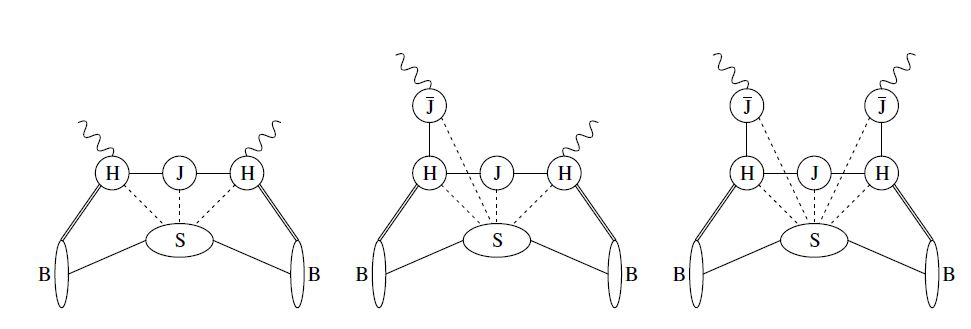
\includegraphics[width=15cm]{Factorization.JPG}
\caption{\label{fig:factorization} Graphical illustration of the factorization for $\bar{B}\rightarrow X_s\gamma$ decay \cite{Benzke:2010js}
}
\end{figure}
Note that this notation is symbolic. Because of this different quantities in different terms can be represented by the same symbol. 

\subsection{Review of the known results}
The factorization formula for the CP-averaged $\bar{B}\rightarrow X_s\gamma$ photon spectrum at the end point region is  
\begin{equation}\label{eqn:chap3_photon_spectrum}
\begin{aligned}
   \frac{d\Gamma}{dE_\gamma} 
   &= \frac{G_F^2\alpha|V_{tb} V_{ts}^*|^2}{2\pi^4}\,
    \overline{m}_b^2(\mu)\,E_\gamma^3\,\Bigg[\,
    |H_\gamma(\mu)|^2 \int_{-p_+}^{\bar\Lambda}\!d\omega\,m_b\,
    J\big( m_b(\omega+p_+),\mu \big)\,S(\omega,\mu) \\
   &\hspace{4.9cm}\mbox{}+ \frac{1}{m_b}\,\sum_{i\le j}\,
    \mbox{Re}\big[C_i^*(\mu)\,C_j(\mu)\big]\,F_{ij}(E_\gamma,\mu)
    + \dots \Bigg] \,,
\end{aligned}
\end{equation}
where $p_{+} \equiv m_{b}-2 E_{\gamma}=\mathcal{O}\left(\Lambda_{\mathrm{QCD}}\right)$, $\bar{\Lambda}$ is defined as $\bar{\Lambda}=M_{B}-m_{b}$ and the ellipses denotes the order $1/m_{b}^2$ terms. The $b$ quark mass is defined in the $\overline{\rm{MS}}$ scheme (see appendix \ref{app:Wilson} ). \par
The first line in the equation represents the leading power contribution, and an extensive discussion regarding this contribution can be found in \cite{Paz:2009ut, Paz:2006me}. The hard function $H_{\gamma}(\mu)$ is the matching coefficient, and it is $H_{\gamma}(\mu)=C_{7\gamma}(\mu)+\mathcal{O(\alpha)}$. In particular, this was obtained by matching the leading current operator to the soft collinear effective field theory (SCET). Also, this current receives contributions from all the operators in the effective Hamiltonian. The dominant contribution is received from $Q_{7\gamma}$, and this is known to $\mathcal{O}(\alpha_s^2)$ \cite{Melnikov:2005bx}. The contributions from the operators other than $Q_{7\gamma}$ are known for $\mathcal{O}(\alpha_s)$ \cite{Benzke:2010js}. The $H_{\gamma}(\mu)$ receives virtual corrections of the scale $\mu_h\sim m_b$.\par
By matching the current operator further onto HQET the single jet function $J\left(p^{2}, \mu\right)=\delta\left(p^{2}\right)+\mathcal{O}\left(\alpha_{s}\right)$ arises. The jet functions describe the cut dependent effects. Specifically, $J\left(p^{2}, \mu\right)$ is obtained by the discontinuity of the quark propagator in the axial gauge \cite{Becher:2006qw}. In particular, the jet function describe the properties of the final state hadronic jet. In the end point region the mass of jet scales as $\mu_{h c} \sim \sqrt{m_{b} \Lambda_{\mathrm{QCD}}}$.\par
The shape function $S(\omega,\mu)$ is a soft function defined by the HQET matrix element \cite{Neubert:1993um}: 
\begin{eqnarray}\label{eqn:chapter3_leading_order_shape_function}
S(\omega, \mu)=\int \frac{d t}{2 \pi} e^{-i \omega t} \frac{\left\langle\bar{B}(v)\left|\bar{h}(t n) S_{n}(t n) S_{n}^{\dagger}(0) h(0)\right| \bar{B}(v)\right\rangle}{2 M_{B}},
\end{eqnarray}  
where the soft Wilson line is defined by
\begin{eqnarray}\label{eqn:chapter3_soft_wilson_line}
S_{n}(x)=\mathbf{P} \exp \left(i g \int_{-\infty}^{0} d u\, n \cdot A_{s}(x+u n)\right).
\end{eqnarray}
The path ordering $\textbf{P}$ in equation (\ref{eqn:chapter3_soft_wilson_line}) means that the fields with larger $u$ value are placed to the left of those fields with smaller $u$ values. The conjugate Wilson line $S^{\dagger}_n$ has the opposite path ordering relative to $S_n$. The combination $S_{n}(t n) S_{n}^{\dagger}(0)=[t n, 0]$ is a straight line segment, which connects the points $tn$ and $0$. The soft function $S$ encodes the nonperturbative hadronic physics associated with the soft scale $\mu_{s} \sim p_{+} \sim \Lambda_{\mathrm{QCD}}$.\par
The power suppressed terms in the equation (\ref{eqn:chap3_photon_spectrum}) are given by \cite{Benzke:2010js}

\begin{align}\label{eqn:chapter3_power_suppressed_terms}
&F_{77}\left(E_{\gamma}, \mu\right)=\frac{C_{F} \alpha_{s}(\mu)}{4 \pi} \int_{-p_{+}}^{\bar{\Lambda}} d \omega\left(16 \ln \frac{m_{b}\left(\omega+p_{+}\right)}{\mu^{2}}+9\right) S(\omega, \mu)+F_{77}^{\mathrm{SSF}}\left(E_{\gamma}, \mu\right)\nonumber\\
&F_{88}\left(E_{\gamma}, \mu\right)=\frac{C_{F} \alpha_{s}(\mu)}{4 \pi} \int_{-p_{+}}^{\bar{\Lambda}} d \omega\left(\frac{2}{9} \ln \frac{m_{b}\left(\omega+p_{+}\right)}{\mu^{2}}-\frac{1}{3}\right) S(\omega, \mu)+4 \pi \alpha_{s}(\mu) f_{88}\left(-p_{+}, \mu\right)\nonumber\\
&F_{78}\left(E_{\gamma}, \mu\right)=\frac{C_{F} \alpha_{s}(\mu)}{4 \pi} \frac{10}{3} \int_{-p_{+}}^{\bar{\Lambda}} d \omega\, S(\omega, \mu)+4 \pi \alpha_{s}(\mu) \operatorname{Re}\left[f_{78}^{(\mathrm{I})}\left(-p_{+}, \mu\right)+f_{78}^{(\mathrm{II})}\left(-p_{+}, \mu\right)\right]\nonumber\\
&F_{17}\left(E_{\gamma}, \mu\right)=\frac{C_{F} \alpha_{s}(\mu)}{4 \pi}\left(-\frac{2}{3}\right) \int_{-p_{+}}^{\bar{\Lambda}} d \omega\, S(\omega, \mu)+\sum_{q=c, u} \delta_{q} \operatorname{Re} f_{17, q}\left(-p_{+}, \mu\right)\nonumber\\
&F_{11}\left(E_{\gamma}, \mu\right)=F_{18}\left(E_{\gamma}, \mu\right)=\frac{C_{F} \alpha_{s}(\mu)}{4 \pi} \frac{2}{9} \int_{-p_{+}}^{\bar{\Lambda}} d \omega S(\omega, \mu),
\end{align}

where 
\begin{eqnarray}
\begin{aligned}
F_{77}^{\mathrm{SSF}}\left(E_{\gamma}, \mu\right)=& p_{+} S\left(-p_{+}, \mu\right)+s\left(-p_{+}, \mu\right)-t\left(-p_{+}, \mu\right)+u\left(-p_{+}, \mu\right)-v\left(-p_{+}, \mu\right) \\
&-\pi \alpha_{s}(\mu)\left[f_{u}^{(s)}\left(-p_{+}, \mu\right)+f_{v}^{(s)}\left(-p_{+}, \mu\right)\right]+\mathcal{O}\left(\frac{\alpha_{s}(\mu)}{4 \pi}\right).
\end{aligned}
\end{eqnarray}
The soft functions in $F_{77}^{\mathrm{SSF}}$ are called subleading shape function, and they describe the direct photon contributions from the operator pair $Q_{7\gamma}-Q_{7\gamma}$ \cite{Bosch:2004cb}. The definitions of the soft functions $S,s,t,u,v,f_u$ and $f_v^{(s)}$ are given as \cite{Bosch:2004cb,Paz:2009ut}:
\begin{eqnarray}\label{eqn:chapter3_soft_fn_ssf}
\begin{aligned}
\left\langle(\bar{h} S)_{0}\left(S^{\dagger} h\right)_{x_{-}}\right\rangle &=\int d \omega e^{-\frac{i}{2} \omega \bar{n} \cdot x} S(\omega) \\
\left\langle i \int d^{4} z T\left\{(\bar{h} S)_{0}\left(S^{\dagger} h\right)_{x_{-}} \mathcal{L}_{h}^{(2)}(z)\right\}\right\rangle &=\frac{1}{m_{b}} \int d \omega e^{-\frac{i}{2} \omega \bar{n} \cdot x} s(\omega) \\
\left\langle\bar{h}(0) \slashed{n} h\left[0, x_{-}\right]\left(i \not D_{\perp} h\right)\left(x_{-}\right)\right\rangle &=\int d \omega \, e^{-\frac{i}{2} \omega \bar{n} \cdot x} t(\omega) \\
-i \int_{0}^{\bar{n} \cdot x / 2} d t\left\langle\bar{h}(0)[0, t n]\left(i D_{\perp}\right)^{2}(t n)\left[t n, x_{-}\right] h\left(x_{-}\right)\right\rangle &=\int d \omega \, e^{-\frac{i}{2} \omega \bar{n} \cdot x} u(\omega) \\
-i \int_{0}^{\bar{n} \cdot x / 2} d t\langle\bar{h}(0) \frac{\slashed{n}}{2}[0, t n] \sigma_{\mu \nu}^{\perp}\, g G_{\perp}^{\mu \nu}(t n)\left[\operatorname{tn}, x_{-}\right] h\left(x_{-}\right)\rangle &=\int d \omega \, e^{-\frac{i}{2} \omega \bar{n} \cdot x} v(\omega),
\end{aligned}
\end{eqnarray} 
and
\begin{eqnarray}
\begin{aligned}
2(-i)^{2} & \int_{0}^{\bar{n} \cdot x / 2} \int_{t_{1}}^{\bar{n} \cdot x / 2} d t_{2}\left\langle\left[(\bar{h} S)_{0} t_{a}\right]_{k}\left[t_{a}\left(S^{\dagger} h\right)_{x_{-}}\right]_{l}\left[(\bar{q} S)_{t_{2} n}\right]_{l} \mu\left[\left(S^{\dagger} q\right)_{t_{1} n}\right]_{k}\right\rangle \\
&=\int d \omega e^{-\frac{i}{2} \omega \bar{n} \cdot x} f_{u}(\omega) \\
\bar{n} \cdot x / 2 & \bar{n} \cdot x / 2 \\
2(-i)^{2} & \int_{0}^{0} d t_{1} \int_{t_{1}}^{\bar{n} \cdot x / 2} d t_{2}\left\langle\left[(\bar{h} S)_{0} t_{a}\right]_{k} \not \mu \gamma_{5}\left[t_{a}\left(S^{\dagger} h\right)_{x_{-}}\right]_{l}\left[(\bar{q} S)_{t_{2} n}\right]_{l} \mu \gamma_{5}\left[\left(S^{\dagger} q\right)_{t_{1} n}\right]_{k}\right\rangle \\
&=\int d \omega e^{-\frac{i}{2} \omega \bar{n} \cdot x} f_{v}(\omega),
\end{aligned}
\end{eqnarray}
where $k$,$l$ are color indices and 
\begin{eqnarray}
\langle\bar{h} \ldots h\rangle \equiv \frac{\langle\bar{B}(v)|\bar{h} \ldots h| \bar{B}(v)\rangle}{2 m_{B}}.
\end{eqnarray}
The term $\mathcal{L}_h$ in equation (\ref{eqn:chapter3_soft_fn_ssf}) is the next-to-leading term in the HQET Lagrangian, which was defined in equation (\ref{Hlag}). Following from this, we find 
\begin{eqnarray}
\mathcal{L}_{h}^{(2)}=\frac{1}{2 m_{b}}\left[\bar{h}\left(i D_{s}\right)^{2} h+\frac{C_{\operatorname{mag}}}{2} \bar{h} \sigma_{\mu \nu} g G_{s}^{\mu \nu} h\right].
\end{eqnarray}
Only the operators $Q_{1}^q-Q_{7\gamma}$, $Q_{7\gamma}-Q_{8g}$ are $Q_{8g}-Q_{8g}$ arise at order $1/m_b$ in equation (\ref{eqn:chap3_photon_spectrum}). The resolved photon contribution provide the largest uncertainty on the decay rate. Because of this, it is important to understand the nature of these operators. In the next section we describe them. 
\subsubsection{Contribution from $Q_1^q-Q_{7\gamma}$}\label{Q1Q7_contr}
\vspace{-0.3cm}
In the equation (\ref{eqn:chapter3_power_suppressed_terms}) the direct photon contributions from $F_{17}$ are given by
\begin{eqnarray}
F_{17}\left(E_{\gamma}, \mu\right)=\frac{C_{F} \alpha_{s}(\mu)}{4 \pi}\left(-\frac{2}{3}\right) \int_{-p_{+}}^{\bar{\Lambda}} d \omega S(\omega, \mu)
\end{eqnarray}
The resolved photon contribution of the operator pair $Q_1^q-Q_{7\gamma}$ is suppressed by a factor $\Lambda_{\mathrm{QCD}} / m_{b}$. By matching this operator pair to the SCET we obtain the diagram in the figure \ref{fig:Q1Q7} (a). Also, by integrating out the (anti)-hard collinear fields we obtain the diagram in the figure \ref{fig:Q1Q7} (b) \cite{Benzke:2010js}.   
\begin{figure}[H]
\subfloat[]{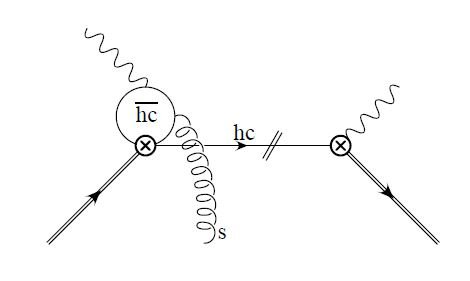
\includegraphics[width = 3in]{Q1Q7a.JPG}}
\subfloat[]{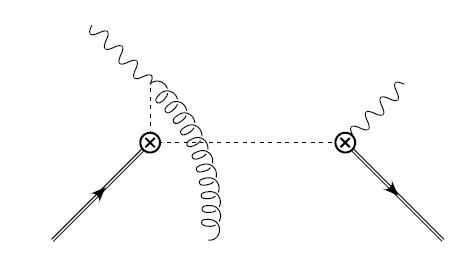
\includegraphics[width = 3in]{Q1Q7b.JPG}}\\
\caption{\label{fig:Q1Q7}Figure (a) represent the diagram arised by matching the $Q_1^q-Q_{7\gamma}$ operator to SCET. Figure (b) represents the diagram obtained by matching same process to HQET \cite{Benzke:2010js}.}
\end{figure}
The single resolved photon contribution of the operator $Q_{1}^q-Q_{7\gamma}$ is given by a non local soft function \cite{Benzke:2010js}
\begin{eqnarray}
\begin{aligned}\label{eqn:chapter3_single_resolved_photon_Q1Q7}
f_{17, q}(\omega, \mu)=\frac{2}{3} \int_{-\infty}^{\infty} \frac{d \omega_{1}}{\omega_{1}+i \varepsilon}\left[1-F\left(\frac{m_{q}^{2}-i \varepsilon}{\left(m_{b}+\omega\right) \omega_{1}}\right)\right] g_{17}\left(\omega, \omega_{1}, \mu\right),
\end{aligned}
\end{eqnarray}
where the penguin function $F$ is defined as 
\begin{eqnarray}\label{eqn:chapter3_penguin_fn}
F(x)=4 x \arctan ^{2}\left(\frac{1}{\sqrt{4 x-1}}\right).
\end{eqnarray}
The expansion of $F(x)$ around $x=0$ is
\begin{eqnarray}\label{eqn:chapter3_F_expansion}
1-F(x)=-\frac{1}{12 x}-\frac{1}{90 x^{2}}-\frac{1}{560 x^{3}}-\dots
\end{eqnarray}
The soft function $g_{17}\left(\omega, \omega_{1}, \mu\right)$  is defined as

\begin{align}\label{eqn:chapter3_suleadinhg_SSf}
g_{17}\left(\omega, \omega_{1}, \mu\right)=& \int \frac{d r}{2 \pi} e^{-i \omega_{1} r} \int \frac{d t}{2 \pi} e^{-i \omega t} \nonumber\\
& \times \frac{\left\langle\bar{B}\left|\left(\bar{h} S_{n}\right)(t n) \vec{\eta}\left(1+\gamma_{5}\right)\left(S_{n}^{\dagger} S_{\bar{n}}\right)(0) i \gamma_{\alpha}^{\perp} \bar{n}_{\beta}\left(S_{\bar{n}}^{\dagger} g G_{s}^{\alpha \beta} S_{\bar{n}}\right)(r \bar{n})\left(S_{\bar{n}}^{\dagger} h\right)(0)\right| \bar{B}\right\rangle}{2 M_{B}},\nonumber\\
\end{align}

where $r$ and $t$ are defined utilizing the topology of the HQET diagrams. For example, the weak vertex in the figure \ref{fig:Q1Q7} (b) is at $x=t n+x_{+}+x_{\perp}$ and the vertex of the soft gluon is defined at $y=r \bar{n}+y_{-}+y_{\perp}$. \par
The variables $\omega$ and $\omega_1$ in equation (\ref{eqn:chapter3_suleadinhg_SSf}) are defined using the light cone projections of parton momenta in $B$ meson. Since the total parton momenta including $b$ quark is equal to $M_B v$, the momentum of the partons in the $B$ meson can be given as 
\begin{eqnarray}
\sum_{i \neq b} n \cdot p_{i}+n \cdot k=\bar{\Lambda}, \quad \sum_{i \neq b} \bar{n} \cdot p_{i}+\bar{n} \cdot k=\bar{\Lambda},
\end{eqnarray}
where $k$ is the residual momentum and $\bar{\Lambda}= M_B-m_b$. Also, note that these light cone projections of parton momenta $n\cdot p_i$ and $\bar{n}\cdot p_i$ are non negative. This provides ($n.k$, $\bar{n}\cdot k)>-m_b$ for $i\neq b$. Besides, it implies $-\infty < n\cdot k\leq\bar{\Lambda}$ and $0 \leq n \cdot p_{i}<\infty$ in the heavy quark limit. These conditions are extended to $\bar{n}\cdot k$ and $\bar{n}\cdot p_i$ as well. Intuitively, the $\omega$ in soft function $g_{17}$ can be thought of as the residual momentum component $n\cdot k$ of the initial state heavy quark. The $\omega_1$ corresponds to either the momentum component $n\cdot p_g$ in final state $B$ meson or the component $-n\cdot p_g$ in initial state $B$ meson. Furthermore, this implies that $-\infty<\omega \leq \bar{\Lambda}$, and $-\infty<\omega_{1}<\infty$.
\par
The direct photon contributions and resolved photon contributions are combined into the final expression for $F_{17}$ in equation (\ref{eqn:chapter3_power_suppressed_terms}) as
\begin{eqnarray}\label{eqn:chapter3_F_17}
F_{17}\left(E_{\gamma}, \mu\right)=\frac{C_{F} \alpha_{s}(\mu)}{4 \pi}\left(-\frac{2}{3}\right) \int_{-p_{+}}^{\bar{\Lambda}} d \omega S(\omega, \mu)+\sum_{q=c, u} \delta_{q} \operatorname{Re} f_{17, q}\left(-p_{+}, \mu\right),
\end{eqnarray}\
where
\begin{eqnarray}
\delta_{q}=\frac{\operatorname{Re}\left[\lambda_{q} C_{1}(\mu)\left(-\lambda_{t}^{*}\right) C_{7 \gamma}^{*}(\mu)\right]}{\left|\lambda_{t}\right|^{2} \operatorname{Re}\left[C_{1}(\mu) C_{7 \gamma}^{*}(\mu)\right]}, \quad \lambda_{q}=V_{q b} V_{q s}^{*}.
\end{eqnarray}
\subsubsection{$Q_{7\gamma}-Q_{8g}$ contribution}
\vspace{-0.3cm}
The direct photon contribution from the operator pair $Q_{7\gamma}-Q_{8g}$ is given by
\begin{eqnarray}
F_{78}^{(a)}\left(E_{\gamma}, \mu\right)=\frac{C_{F} \alpha_{s}(\mu)}{4 \pi} \frac{m_{b}}{2 E_{\gamma}} \frac{10}{3} \int_{-p_{+}}^{\bar{\Lambda}} d \omega S(\omega, \mu)
\end{eqnarray}
The operator $Q_{8g}$ provides two SCET operators, and these operators are combined with the tree level SCET operator arising in $Q_{7\gamma}$. These two operators provide the $Q_{7\gamma}-Q_{8g}$ contribution.
Figure \ref{fig:Q1Q8} was obtained by matching the SCET operators onto HQET operators  \cite{Benzke:2010js}.
\begin{figure}[H]
\subfloat[]{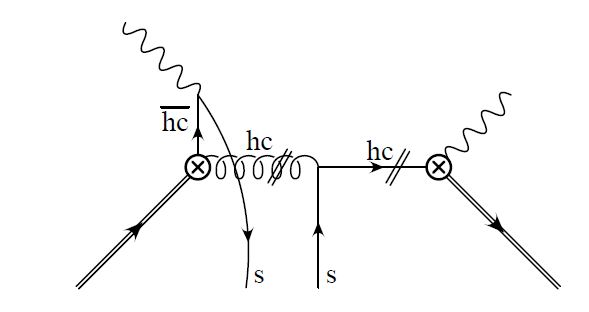
\includegraphics[width = 2.75in]{Q7Q8a.JPG}}
\subfloat[]{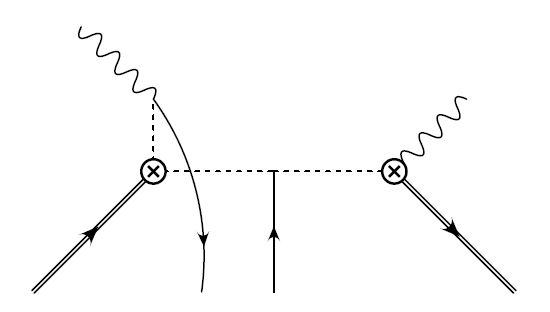
\includegraphics[width = 2.75in]{Q7Q8b.JPG}}\\
\subfloat[]{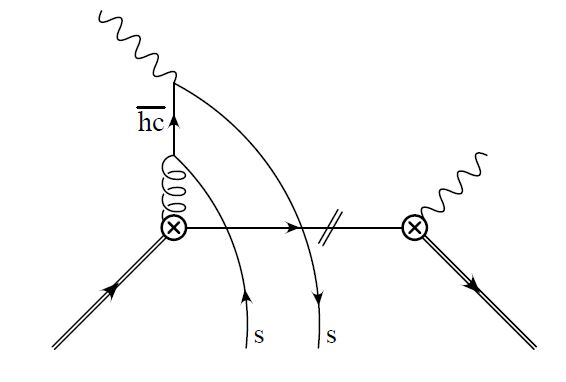
\includegraphics[width = 2.75in]{Q7Q8c.JPG}}
\subfloat[]{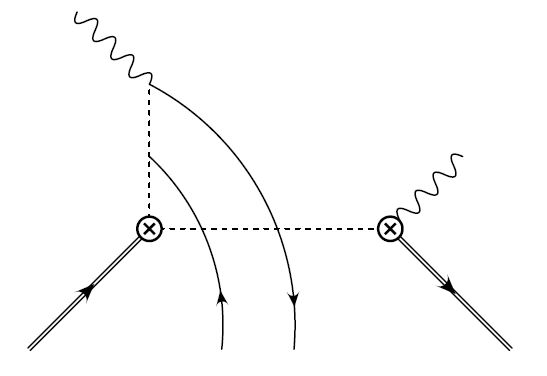
\includegraphics[width = 2.75in]{Q7Q8d.JPG}}
\caption{\label{fig:Q1Q8}Figure (a) and (c) represent the diagrams arised by matching the $Q_{7\gamma}-Q_{8g}$ operator to SCET. Figure (b) and (d) represents the diagrams obtained by matching same processes to HQET \cite{Benzke:2010js}.}
\end{figure} 
The contribution from the operator pair $Q_{7\gamma}-Q_{8g}$ to the photon spectrum is provided as \cite{Benzke:2010js}
\begin{eqnarray}
\begin{aligned}
F_{78}\left(E_{\gamma}, \mu\right)=& \frac{C_{F} \alpha_{s}(\mu)}{4 \pi} \frac{m_{b}}{2 E_{\gamma}} \frac{10}{3} \int_{-p_{+}}^{\bar{\Lambda}} d \omega S(\omega, \mu) \\
&+4 \pi \alpha_{s}(\mu) \frac{m_{b}}{2 E_{\gamma}} \operatorname{Re}\left[f_{78}^{(\mathrm{I})}\left(-p_{+}, \mu\right)+f_{78}^{(\mathrm{II})}\left(-p_{+}, \mu\right)\right],
\end{aligned}
\end{eqnarray}
where $f^{(\rm{I})}$ and $f^{(\rm{II})}$ are soft functions that encode the long distance physics. Unfortunately there is little information on these functions. The effect of these soft functions can be roughly approximated using \textit{vacuum insertion approximation} (VIA). In VIA, the matrix elements are evaluated by inserting vacuum states between light quark fields. Since the $Q_{7\gamma}-Q_{8g}$ operators involve light quark fields, the vacuum insertion model provides an estimate to the matrix element. Using the VIA model $f^{(\rm{I})}$ and $f^{(\rm{II})}$ as obtained as \cite{Benzke:2010js}

\begin{align}
\left.\int_{-\infty}^{\bar{\Lambda}} d \omega f_{78}^{(\mathrm{II})}(\omega, \mu)\right|_{\mathrm{VIA}} &=-e_{\mathrm{spec}} \frac{F^{2}(\mu)}{8}\left(1-\frac{1}{N_{c}^{2}}\right)\left\{\frac{1}{\lambda_{B}^{2}(\mu)}+2 \pi i \int_{0}^{\infty} d \omega \frac{\left[\phi_{+}^{B}(\omega, \mu)\right]^{2}}{\omega}\right\}\nonumber \\
\left.\int_{-\infty}^{\bar{\Lambda}} d \omega \operatorname{Re} f_{78}^{(\mathrm{II})}(\omega, \mu)\right|_{\mathrm{VIA}} &=-e_{\mathrm{spec}} \frac{F^{2}(\mu)}{8}\left(1-\frac{1}{N_{c}^{2}}\right) \frac{1}{\lambda_{B}^{2}(\mu)}, 
\end{align}

where $\lambda_{B}=\int_{0}^{\infty} d \omega \phi_{+}^{B}(\omega, \mu) / \omega$ and $\phi_{+}^{B}$ is the leading light cone distribution amplitude \cite{Grozin:1996pq}. The nonperturbative quantity $F(\mu)$ is the HQET matrix element that relates to the asymptotic value of $f_{B} \sqrt{M_{B}}|_{M_b\rightarrow \infty}$ and $f_B$ is the $B$ meson decay constant.
\vspace{-0.3cm}
\subsubsection{$Q_{8g}-Q_{8g}$ contribution} 
\vspace{-0.3cm}
The direct photon contribution of $Q_{8g}-Q_{8g}$ is given by \cite{Benzke:2010js}
\begin{eqnarray}\label{eqn:chapter3_Q8Q8_dir}
F_{88}^{(a)}\left(E_{\gamma}, \mu\right)=\frac{C_{F} \alpha_{s}(\mu)}{4 \pi}\left(\frac{m_{b}}{2 E_{\gamma}}\right)^{2} \int_{-p_{+}}^{\bar{\Lambda}} d \omega\left(\frac{2}{9} \ln \frac{m_{b}\left(\omega+p_{+}\right)}{\mu^{2}}+\frac{1}{9}-\frac{4}{9} c_{\mathrm{RS}}\right) S(\omega, \mu),
\end{eqnarray}
where $c_{\rm{RS}}$ is a scheme dependent coefficient. For instance, in $\bar{\rm{MS}}$ scheme $c_{\bar{\rm{MS}}}=0$. In the dimensional reduction scheme, which set $d=4$ instead of $d=4-2\epsilon$ for Dirac algebra, the $c_{\rm{DR}}=1$. The equation (\ref{eqn:chapter3_Q8Q8_dir}) is further simplified as 
\begin{eqnarray}
F_{88}^{(a)}\left(E_{\gamma}, \mu\right)=\frac{C_{F} \alpha_{s}(\mu)}{4 \pi}\left(\frac{m_{b}}{2 E_{\gamma}}\right)^{2} \int_{-p_{+}}^{\bar{\Lambda}} d \omega\left(\frac{2}{9} \ln \frac{m_{b}\left(\omega+p_{+}\right)}{\mu^{2}}-\frac{1}{3}\right) S(\omega, \mu),
\end{eqnarray}
The $Q_{8g}-Q_{8g}$ receives double resolved photon contributions. This is shown in the figure \ref{fig:Q8Q8}

\begin{figure}[H]
\subfloat[]{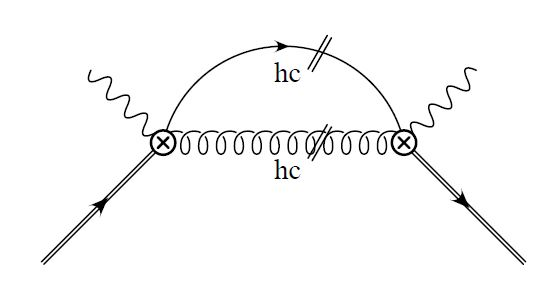
\includegraphics[width = 3in]{Q8Q8a.JPG}}
\subfloat[]{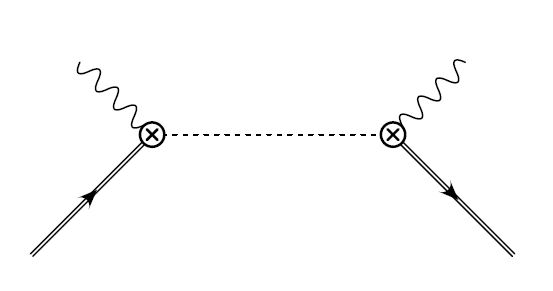
\includegraphics[width = 3in]{Q8Q8b.JPG}}\\
\subfloat[]{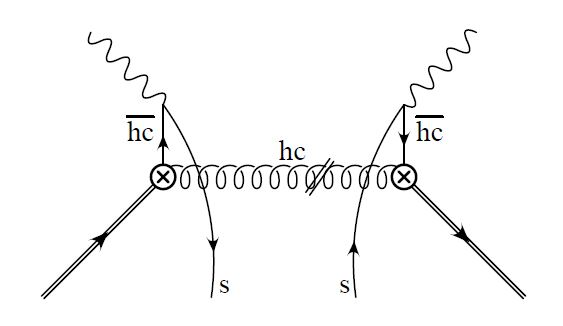
\includegraphics[width = 3in]{Q8Q8c.JPG}}
\subfloat[]{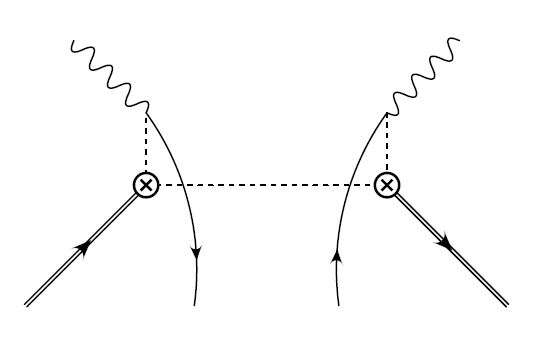
\includegraphics[width = 3in]{Q8Q8d.JPG}}
\caption{\label{fig:Q8Q8}Figure (a) and (c) represent the diagrams arised by matching the $Q_{8\gamma}-Q_{8g}$ operator to SCET. Figure (b) and (d) represents the diagrams obtained by matching same processes to HQET \cite{Benzke:2010js}.}
\end{figure} 
The double resolved contribution to the photon spectrum is given by \cite{Benzke:2010js}
\begin{eqnarray}
F_{88}^{(b)}\left(E_{\gamma}, \mu\right)=4 \pi \alpha_{s}(\mu)\left(\frac{m_{b}}{2 E_{\gamma}}\right)^{2} f_{88}\left(-p_{+}, \mu\right),
\end{eqnarray}
where $f_{88}$ encodes the long distance physics. This function is defined as 
\begin{eqnarray}
f_{88}(\omega, \mu)=\frac{2}{9} \int_{-\infty}^{\infty} \frac{d \omega_{1}}{\omega_{1}+i \varepsilon} \int_{-\infty}^{\infty} \frac{d \omega_{2}}{\omega_{2}-i \varepsilon} g_{88}^{\mathrm{cut}}\left(\omega, \omega_{1}, \omega_{2}, \mu\right),
\end{eqnarray}
where non-local matrix element $ g_{88}^{\mathrm{cut}}$ is given by

\begin{align}\label{eqn:chapter3_g88}
&g_{88}^{\mathrm{cut}}\left(\omega, \omega_{1}, \omega_{2}, \mu\right)\nonumber\\
=& \int \frac{d r}{2 \pi} e^{-i \omega_{1} r} \int \frac{d u}{2 \pi} e^{i \omega_{2} u} \int \frac{d t}{2 \pi} e^{-i \omega t}\nonumber \\
& \times \frac{\left\langle\bar{B}\left|\left(\bar{h} S_{n}\right)(t n) T^{A}\left(S_{n}^{\dagger} S_{\bar{n}}\right)(\operatorname{tn}) \bar{\Gamma}_{\bar{n}}\left(S_{\bar{n}}^{\dagger} s\right)(t n+u \bar{n})\left(\bar{s} S_{\bar{n}}\right)(r \bar{n}) \Gamma_{\bar{n}}\left(S_{\bar{n}}^{\dagger} S_{n}\right)(0) T^{A}\left(S_{n}^{\dagger} h\right)(0)\right| \bar{B}\right\rangle}{2 M_{B}}
\end{align}

The matrix element in equation (\ref{eqn:chapter3_g88}) is obtained by summing over soft intermediate states with strangeness $S=-1$ ($\mathcal{X}_{s}$).
\subsection{Resolved photon contributions to the total rate}
If the photon spectrum is integrated over a much larger interval in the phase space than the end point region (integrated rate), then the direct photon contributions can be further simplified. Typically, the direct photon contributions are given by a series of hard coefficients that are multiplyed by a set of forward $B$ meson matrix elements of local operators. The correction terms of order $\frac{\Lambda_{\rm{QCD}}}{m_b}$ are integrated to zero. This is due to the abscence of local gauge operators that can account such terms at the order $\frac{\Lambda_{\rm{QCD}}}{m_b}$. However, the resolved photon contributions do not reduced to such matrix elements of local operators \cite{Benzke:2010js}. The effects of these operators on total rate should be addressed by using non-local operators \cite{Lee:2006wn}\par
As shown in \cite{Benzke:2010js}, single resolved photon contributions arise from the operator pairs $Q_{8g}-Q_{7\gamma}$ and $Q_{1}^{c}-Q_{7\gamma}$. In addition, double resolved photon contributions arise from the operator pairs  $Q_{8g}-Q_{8g}$, $Q_{1}^{c}-Q_{1}^{c}$ and $Q_{1}^{c}-Q_{8g}$. Direct photon contributions arise from all the operator pairs.\par
The breakdown of the operators in leading order, next-to-leading order, and next-to-next-to-leading order in HQET power counting is as follows:
\begin{itemize}
  \item The contribution of the operators  $Q_{7\gamma}-Q_{7\gamma}$ is the leading power correction. 
  \item The operators $Q_{1}^{q}-Q_{7\gamma}$, $Q_{8g}-Q_{8g}$ and $Q_{8g}-Q_{7\gamma}$, are order $1/m_{b}$ in the power corrections. 
  \item The operators $Q_{1}^{c}-Q_{1}^{c}$ and $Q_{1}^{c}-Q_{8g}$ contribute at order $1/m^{2}_{b}$. Since our primary focus is on improving the order $1/m_b$ corrections, we do not consider these order $1/m^{2}_{b}$ operators in our analysis.
\end{itemize}
In the following, we discuss these order  $1/m_b$ corrections.
\subsection{Contribution from nonperturbative correction}\label{sec:nonpert_contr}
The function $\mathcal{F}_E$ quantifies the effects of resolved photon contributions to the total rate \cite{Benzke:2010js}
\begin{eqnarray}
\mathcal{F}_{E}(\Delta)=\frac{\Gamma(E_0)-\Gamma(E_0)|_{\rm{OPE}}}{\Gamma(E_0)|_{\rm{OPE}}},
\end{eqnarray} 
where $\Delta=m_{b}-2 E_{0}$. The $\Gamma(E_0)|_{\rm{OPE}}$ \cite{Misiak:2006zs} is obtained by a local operator product expansion, which does not consider the nonlocal power corrections from resolved photon contributions. The contribution from $1/m_b$ operators is
\begin{eqnarray}\label{eqn:chapter3_resolved_photon_err}
\begin{aligned}
\begin{aligned}
\mathcal{F}_{E}(\Delta)=& \frac{C_{1}(\mu)}{C_{7 \gamma}(\mu)} \frac{\Lambda_{17}\left(m_{c}^{2} / m_{b}, \mu\right)}{m_{b}}+\frac{C_{8 g}(\mu)}{C_{7 \gamma}(\mu)} 4 \pi \alpha_{s}(\mu) \frac{\Lambda_{78}^{\mathrm{spec}}(\mu)}{m_{b}} \\
&+\left(\frac{C_{8 g}(\mu)}{C_{7 \gamma}(\mu)}\right)^{2}\left[4 \pi \alpha_{s}(\mu) \frac{\Lambda_{88}(\Delta, \mu)}{m_{b}}-\frac{C_{F} \alpha_{s}(\mu)}{9 \pi} \ln \frac{\Delta}{m_{b}}\right]+\ldots,
\end{aligned}
\end{aligned}
\end{eqnarray}
where 

\begin{align}\label{eqn:chapter3_soft_functions}
\Lambda_{17}\left(\frac{m_{c}^{2}}{m_{b}}, \mu\right) &=e_{c} \operatorname{Re} \int_{-\infty}^{\infty} \frac{d \omega_{1}}{\omega_{1}}\left[1-F\left(\frac{m_{c}^{2}-i \varepsilon}{m_{b} \omega_{1}}\right)+\frac{m_{b} \omega_{1}}{12 m_{c}^{2}}\right] h_{17}\left(\omega_{1}, \mu\right)\nonumber \\
\Lambda_{78}^{\mathrm{spec}}(\mu) &=\operatorname{Re} \int_{-\infty}^{\infty} \frac{d \omega_{1}}{\omega_{1}+i \varepsilon} \int_{-\infty}^{\infty} \frac{d \omega_{2}}{\omega_{2}-i \varepsilon} h_{78}^{(5)}\left(\omega_{1}, \omega_{2}, \mu\right)\nonumber \\
\Lambda_{88}(\Delta, \mu) &=e_{s}^{2}\left[\int_{-\infty}^{\Lambda_{\mathrm{UV}}} \frac{d \omega_{1}}{\omega_{1}+i \varepsilon} \int_{-\infty}^{\Lambda_{\mathrm{UV}}} \frac{d \omega_{2}}{\omega_{2}-i \varepsilon} 2 h_{88}^{\mathrm{cut}}\left(\Delta, \omega_{1}, \omega_{2}, \mu\right)-\frac{C_{F}}{8 \pi^{2}} \Delta\left(\ln \frac{\Lambda_{\mathrm{UV}}}{\Delta}-1\right)\right].
\end{align}

The functions $h_{17}, h_{88}$ and $h_{78}$ are non-local HQET matrix elements that encode the long-distance nonperturbative effects\cite{Benzke:2010js}. These soft functions cannot be determined from the first principles, and the evaluation of their contribution to the total rate requires modeling. In the following, we provide a concise review regarding past evaluations their contribution. 
\vspace{-0.4cm}
\subsubsection{Estimating $\mathcal{F}_E|_{17}$}\label{sec:Q1Q7_cont}
\vspace{-0.2cm}
In equation (\ref{eqn:chapter3_soft_functions}) the soft function $h_{17}$ is defined as

\begin{eqnarray}\label{eqn:chapetr3_h_17}
\begin{aligned}
h_{17}\left(\omega_{1}, \mu\right) &=\int_{-\Delta}^{\bar{\Lambda}} d \omega g_{17}\left(\omega, \omega_{1}, \mu\right) \approx \int_{-\infty}^{\bar{\Lambda}} d \omega g_{17}\left(\omega, \omega_{1}, \mu\right) \\
&=\int \frac{d r}{2 \pi} e^{-i \omega_{1} r} \frac{\left\langle\bar{B}\left|\left(\bar{h} S_{\bar{n}}\right)(0) \slashed{\bar{n}} i \gamma_{\alpha}^{\perp} \bar{n}_{\beta}\left(S \frac{\dagger}{n} g G_{s}^{\alpha \beta} S_{\bar{n}}\right)(r \bar{n})\left(S_{\bar{n}}^{\dagger} h\right)(0)\right| \bar{B}\right\rangle}{2 M_{B}}
\end{aligned}
\end{eqnarray} 
\vspace{0.1cm}

The moments of the function $h_{17}$ in equation (\ref{eqn:chapetr3_h_17}) are related to the nonperturbative HQET parameters. Based on this feature, we can construct phenomenological models to describe this non-local function. For instance, in \cite{Benzke:2010js} there were several phenomenological models for function $h_{17}$ that are related to the zeroth moment of $h_{17}$ over $\omega_1$ ($\langle \omega_1^0 h_{17}(\omega_1)\rangle$). Consider the following model
\begin{eqnarray}\label{eqn:chapter3_old_model}
h_{17}\left(\omega_{1}, \mu\right)=\frac{2 \lambda_{2}}{\sqrt{2 \pi} \sigma} \frac{\omega_{1}^{2}-\Lambda^{2}}{\sigma^{2}-\Lambda^{2}} e^{-\frac{\omega_{1}^{2}}{2 \sigma^{2}}},
\end{eqnarray}
where $\sigma$ is the width of the Gaussian function and $\Lambda$ is a ad-hoc parameter. Scanning through different values for $\sigma$ and $\Lambda$ in $h_{17}$ the maximum and minimum values for $\Lambda_{17} $ obtained as \cite{Benzke:2010js}
\begin{eqnarray}
-60 \mathrm{MeV}<\Lambda_{17}<25 \mathrm{MeV}.
\end{eqnarray} 
Based on this estimate of $\Lambda_{17}$ the $\mathcal{F}_E|_{17}$ from equation (\ref{eqn:chapter3_resolved_photon_err})
\begin{eqnarray}
\mathcal{F}_E|_{17}=\frac{C_{1}(\mu)}{C_{7 \gamma}(\mu)} \frac{\Lambda_{17}\left(m_{c}^{2} / m_{b}, \mu\right)}{m_{b}}
\end{eqnarray}
\subsubsection{Estimating $\mathcal{F}_E|_{78}$}\label{subsec:F_78}
\vspace{-0.2cm}
The contribution of the operator pair $Q_{7\gamma}-Q_{8g}$ is obtained by using the flavor symmetry of the strong interaction. The flavor averaged estimate of the $\mathcal{F}_E|_{78}$ is given by \cite{Benzke:2010js}

\begin{eqnarray}\label{eqn:chapter3_78_contribution}
\left.\mathcal{F}_{E}^{\mathrm{avg}}(\Delta)\right|_{7 8}=-(1 \pm 0.3) \frac{\Delta_{0-}}{3},
\end{eqnarray}

where $\Delta_{0-}$ is the isospin asymmetry, which is given by

\begin{eqnarray}
\Delta_{0-}=\frac{\Gamma\left(\bar{B}^{0} \rightarrow X_{s} \gamma\right)-\Gamma\left(B^{-} \rightarrow X_{s} \gamma\right)}{\Gamma\left(\bar{B}^{0} \rightarrow X_{s} \gamma\right)+\Gamma\left(B^{-} \rightarrow X_{s} \gamma\right)}
\end{eqnarray}

Also, $\mathcal{F}_E|_{78}$ can be evaluated by using the vacuum insertion approximation (VIA). From equation (\ref{eqn:chapter3_resolved_photon_err})
 
\begin{eqnarray}
\mathcal{F}_E|_{78}= \frac{C_{8 g}(\mu)}{C_{7 \gamma}(\mu)} 4 \pi \alpha_{s}(\mu) \frac{\Lambda_{78}^{\mathrm{spec}}(\mu)}{m_{b}}, 
\end{eqnarray}

In the unbrocken $SU(3)$ flavor symmetry limit, the nonperturbative parameter $\Lambda_{78}^{\mathrm{spec}}$ is 
\begin{eqnarray}\label{eqn:chapter3_Lamda_78}
\left.\Lambda_{78}^{\mathrm{spec}}\right|_{S U(3)}=e_{\mathrm{spec}} \Lambda_{I=1}^{(8)},
\end{eqnarray}
where $e_{\rm{spec}}$ is the electric charge of the spectator quark (i.e $e_{\rm{spec}}=2/3$ for $B^{\pm}$ and $e_{\rm{spec}}=-1/3$ for $B^{0}(\bar{B}^{0})$). The soft function that encodes the long distance physics from $Q_{7\gamma}-Q_{8g}$ operator pair can be written as a $SU(3)$ octet matrix element. The Wigner-Ekchart theorem is used to decompose the matrix element  into isospin zero and isospin one components. The $\Lambda_{I=1}^{(8)}$ is the isospin 1 component of the $SU(3)$ octet. Using the VIA the estimate for $\Lambda_{I=1}^{(8)}$ is obtained as $\Lambda_{I=1}^{(8)}|_{\rm{VIA}}\in [-386,-35]\text{ MeV}$ \cite{Benzke:2010js}. This estimate is used in equation (\ref{eqn:chapter3_Lamda_78}) to obtain $\mathcal{F}_E|_{78}$.
\vspace{-0.3cm}
\subsubsection{Estimating $\mathcal{F}_E|_{88}$}\label{subsec:F_88}
\vspace{-0.2cm}
In equation (\ref{eqn:chapter3_resolved_photon_err}) the contribution from operator pair $Q_{8g}-Q_{8g}$ is 
\begin{eqnarray}\label{eqn:chapter3_Q8Q8}
\mathcal{F}_E|_{78}=\left(\frac{C_{8 g}(\mu)}{C_{7 \gamma}(\mu)}\right)^{2}\left[4 \pi \alpha_{s}(\mu) \frac{\Lambda_{88}(\Delta, \mu)}{m_{b}}-\frac{C_{F} \alpha_{s}(\mu)}{9 \pi} \ln \frac{\Delta}{m_{b}}\right].
\end{eqnarray}
\vspace{0.2cm}
Compared to the first term, the second term in the equation (\ref{eqn:chapter3_Q8Q8}) provides a very small contribution to the $\mathcal{F}_E|_{78}$ \cite{Benzke:2010js}. The first term in $\mathcal{F}_E|_{78}$ is defined using the nonperturabtive function $\Lambda_{88}$, which was defined in equation (\ref{eqn:chapter3_soft_functions}). Currently there is not much information on the soft function that describes $\Lambda_{88}$, and it is, however, estimated by \cite{Benzke:2010js} 
\begin{eqnarray}
\Lambda_{88}(\Delta, \mu) \approx e_{s}^{2} \Lambda(\mu), \quad \Lambda(\mu)>0,
\end{eqnarray}
where $\Lambda(\mu)$ is a parameter of order $\Lambda_{\mathrm{QCD}}$. The electromagnetic charge of the $s$ quark gives $e^2_s=\frac{1}{9}$. The range of the $\Lambda(\mu)$ is defined as $0<\Lambda(\mu)<1\text{ GeV}$ \cite{Benzke:2010js}. Based on this range the phenomenological estimate for the $\mathcal{F}_E|_{88}$ was obtained.
\vspace{-0.3cm}
\subsubsection{Phenomenological estimates of theoretical error}
\vspace{-0.2cm}
At order $1/m_{b}$, $\mathcal{F}_E$ depends on $Q_{1}-Q_{7\gamma}$, $Q_{8g}-Q_{8g}$ and $Q_{8g}-Q_{7\gamma}$; The contribution from each of these operators were obtained by Benzke \textit{et al.} (2010)\cite{Benzke:2010js}: 
\begin{eqnarray}\label{eqn:chapter3_error_est}
\begin{aligned}
&\left.\mathcal{F}_{E}\right|_{17} \in[-1.7,+4.0] \%\\
&\left.\mathcal{F}_{E}\right|_{88} \in[-0.3,+1.9] \%
\end{aligned}
\end{eqnarray}
and
\begin{eqnarray}
\begin{array}{l}
{\left.\mathcal{F}_{E}\right|_{78} ^{\mathrm{VIA}} \in[-2.8,-0.3] \%} \\
{\left.\mathcal{F}_{E}\right|_{78} ^{\mathrm{exp}} \in[-4.4,+5.6] \% \quad(95 \% \mathrm{CL})}
\end{array}
\end{eqnarray}
In total, the estimate for ${\cal F}_E$ is obtained by using both experimental and theoretical estimates of $\Lambda_{78}^{\rm{spec}}$. For instance, the 2010 theoretical estimate of uncertainty using VIA is \cite{Benzke:2010js}.

\begin{equation}\label{Fcurrentexp}
   -4.8 \%<\mathcal{F}_{E}(\Delta)<+5.6 \% \quad\left(\mathrm{VIA} \text { for } \Lambda_{78}^{\mathrm{spec}}\right).
\end{equation}
Here the estimate for $\mathcal{F}_E|^{\rm{VIA}}_{78}$ is obtained by plugging the value of $\Lambda_{I=1}^{(8)}|^{\rm{VIA}}$.\par
The 2010 estimate of $\Lambda_{78}^{\rm{spec}}$, which is obtained using isospin asymmetry $\Delta_{0-}$, is given by
\begin{eqnarray}\label{eqn:F78_using_exp}
-6.4 \%<\mathcal{F}_{E}(\Delta)<+11.5 \% \quad\left(\Lambda_{78}^{\mathrm{spec}} \text { from } \Delta_{0-}\right),
\end{eqnarray}
where $\Delta_{0-}=(-1.3 \pm 5.9) \%$, which was measured by BaBar collaboration \cite{Aubert:2005cua, Aubert:2007my}, and the uncertainty of $\Delta_{0-}$ is $95\%$ confidence level (CL) \cite{Benzke:2010js}. 

\section{The CP asymmetry}
The CP violation (CPV) due to direct photon in $\bar{B}\rightarrow X_s\gamma$ arises by the interference of a weak phases in the CKM matrix elements and the possible BSM corrections to Wilson coefficients with the strong phases arising in the process \cite{Kagan:1998bh}. These strong phases can be obtained by calculating the imaginary parts of the local operators in the effective Hamiltonian given in equation (\ref{eq:Weak Hamiltonian}). For instance, the imaginary parts first arise at $\mathcal{O}(\alpha_s)$ in loop diagrams that contains $c$ quarks or light partons \cite{Kagan:1998bh}.
The CP asymmetry is given by \cite{Benzke:2010tq},
\begin{equation}\label{data}
   {\cal A}_{X_s\gamma} 
   = \frac{\Gamma(\bar B\to X_s\gamma)-\Gamma(B\to X_{\bar s}\gamma)}%   
          {\Gamma(\bar B\to X_s\gamma)+\Gamma(B\to X_{\bar s}\gamma)} \,.
\end{equation}
In \cite{Benzke:2010tq} the SM estimate for CP asymmetry is provided as    
\begin{eqnarray}
-0.6\%< \mathcal{A}_{X_s\gamma}^{\rm{SM}}<2.8\%
\end{eqnarray}
This estimate is compared to the PDG average  of the experimental measurement $1.5 \% \pm 1.1 \%$ \cite{Tanabashi:2018oca}. These were first considered in \cite{Benzke:2010tq}.
The resolved photon contributions that arise in the photon spectrum is important to the analysis of the direct CP asymmetry.
\par
The experimental measurement of the CP asymmetry ($\mathcal{A}_{X_{s} \gamma}\left(E_{0}\right)$) depend on the photon cut $E_{\gamma}\geq E_0$. Where $E_0$ is in the range $1.9\text{ GeV}<E_0<2.2\text{ GeV}$, and $\Delta= m_b-2E_0= \rm{few}\times\Lambda_{\rm{QCD}}$ \cite{Benzke:2010tq}. This cut related CP asymmetry is known as \textit{partially inclusive} asymmetry \cite{Benzke:2010tq}. The direct photon contributions to the CP asymmetry can be expressed by using a power series in $\Delta/m_b$ and $\Lambda_{\rm{QCD}}/\Delta$. At the $\mathcal{O}(\alpha_s)$, the direct photon contribution to $\mathcal{A}_{X_{s} \gamma}$ is

\begin{eqnarray}\label{eqn:chapter3_dir_photon_CP}
   {\cal A}_{X_s\gamma}^{\rm dir}
   &=& \alpha_s\,\Bigg\{ \frac{40}{81}\,\mbox{Im}\frac{C_1}{C_{7\gamma}}
    - \frac49\,\mbox{Im}\frac{C_{8g}}{C_{7\gamma}}- \frac{40\Lambda_c}{9m_b}\,\mbox{Im}\bigg[(1+\epsilon_s)\,
    \frac{C_1}{C_{7\gamma}}\bigg] 
    + {\cal O}\bigg( \frac{\Lambda_{\rm QCD}^2}{m_b^2} \bigg) \Bigg\} \,, 
\end{eqnarray}
where the $C_1, C_{7\gamma}$ and $C_{8g}$ are the Wilson coefficients (effective couplings) of current-current four quark operator ($Q_{1}^q$), electromagnetic dipole operator ($Q_{7\gamma}$) and gluon dipole operator ($Q_{8g}$) respectively. Also, the parameter $\Lambda_{c}$ is defined as 
\begin{eqnarray}\label{eqn:chapter3_Lambda_C}
\Lambda_{c} \equiv \frac{m_{c}^{2}}{m_{b}}\left(1-\frac{2}{5} \ln \frac{m_{b}}{m_{c}}+\frac{4}{5} \ln ^{2} \frac{m_{b}}{m_{c}}-\frac{\pi^{2}}{15}\right),
\end{eqnarray}
The $\Lambda_c\sim\Lambda_{\rm{QCD}}$ is obtained by plugging $m_b=4.65\text{ GeV}$ and $m_c=1.13\text{ GeV}$ in equation (\ref{eqn:chapter3_Lambda_C}). Following from this we obtain $\Lambda_c\sim 0.38 \text{ GeV}$. The parameter $\epsilon_s$ is the ratio of CKM matrix elements, and it is defined as \cite{Kagan:1998bh}
\begin{eqnarray}
\epsilon_{s}=\frac{v_{u}}{v_{t}}=\frac{V_{u s}^{*} V_{u b}}{V_{t s}^{*} V_{t b}} \approx \lambda^{2}(i \eta-\rho)=O\left(10^{-2}\right),
\end{eqnarray}
where the parameters $\lambda,\rho$ and $\eta$ are Wolfenstein parameters defined as $\lambda=\sin \theta_{\mathrm{C}} \approx 0.22$ and $\rho, \eta=\mathcal{O}(1)$. Only the third term in the equation (\ref{eqn:chapter3_dir_photon_CP}) is non-zero in the SM. This term is triply suppressed by the $\alpha_s$, $\rm{Im}(\epsilon_s)$ and $(m_c/m_b)^2\sim \Lambda_{\rm{QCD}}/m_b$.

\subsection{Resolved photon contributions to the CP asymmetry}\label{sec:resolved_cp_A}
Using the factorization formula provided in equation (\ref{eqn:btoxgam_fact}) the effects of resolved photon operators to the partially inclusive CP asymmetry can be evaluated. For instance, these nonlocal effects arise from the interference of $Q_{7\gamma}-Q_{7\gamma}$ amplitude with $Q_{1}^{(u,c)}-Q_{7\gamma}$ and $Q_{7\gamma}-Q_{8g}$ amplitudes. Following from this, the resolved photon contribution to the CP asymmetry is obtained as
\begin{eqnarray}\label{eqn:chapter3_resolved_contr_CPA}
   {\cal A}_{X_s\gamma}^{\rm res}
   &=& \frac{\pi}{m_b}\,\bigg\{
    \mbox{Im}\bigg[(1+\epsilon_s)\,\frac{C_1}{C_{7\gamma}}\bigg]\,\tilde\Lambda_{17}^c 
    - \mbox{Im}\bigg[\epsilon_s\,\frac{C_1}{C_{7\gamma}}\bigg]\,\tilde\Lambda_{17}^u +\mbox{Im}\,\frac{C_{8g}}{C_{7\gamma}}\,
    4\pi\alpha_s\,\tilde\Lambda_{78}^{\bar B} \bigg\} \,,
\end{eqnarray}
where 
\begin{eqnarray}
\begin{aligned}
&\tilde{\Lambda}_{17}^{u}=\frac{2}{3} h_{17}(0)\\
&\tilde{\Lambda}_{17}^{c}=\frac{2}{3} \int_{4 m_{c}^{2} / m_{b}}^{\infty} \frac{d \omega}{\omega} f\left(\frac{m_{c}^{2}}{m_{b} \omega}\right) h_{17}(\omega)\\
&\tilde{\Lambda}_{78}^{\bar{B}}=2 \int_{-\infty}^{\infty} \frac{d \omega}{\omega}\left[h_{78}^{(1)}(\omega, \omega)-h_{78}^{(1)}(\omega, 0)\right]
\end{aligned}
\end{eqnarray}
and 
\begin{eqnarray}
f(x)=2 x \ln \frac{1+\sqrt{1-4 x}}{1-\sqrt{1-4 x}}.
\end{eqnarray}

In the unbroken $SU(3)$ limit, the $\tilde{\Lambda}_{78}$ is defined as
\begin{eqnarray}
\tilde{\Lambda}_{78}^{\bar{B}} \approx e_{\text {spec }} \tilde{\Lambda}_{78} \approx e_{\text {spec }} \frac{2 f_{B}^{2} M_{B}}{9} \int_{0}^{\infty} d \omega \frac{\left[\phi_{+}^{B}(\omega)\right]^{2}}{\omega},
\end{eqnarray}
where the $f_{B}$ is the $B$ meson decay constant and it is evaluated as $f_{B}\approx 193\text{ MeV}$ \cite{Benzke:2010tq}. The $\phi_{+}^{B}$ is the leading light cone distribution amplitude \cite{Grozin:1996pq}. Using the models provided in sections \ref{sec:Q1Q7_cont} and \ref{subsec:F_88} the parameters $\tilde{\Lambda}_{ij}$ can be obtained \cite{Benzke:2010tq}
\vspace*{-0.6cm}
\begin{eqnarray}
\begin{aligned}
-330 \mathrm{MeV} &<\tilde{\Lambda}_{17}^{u}<+525 \mathrm{MeV}, \\
-9 \mathrm{MeV} &<\tilde{\Lambda}_{17}^{c}<+11 \mathrm{MeV}, \\
17 \mathrm{MeV} &<\tilde{\Lambda}_{78}<190 \mathrm{MeV}.
\end{aligned}
\vspace*{-0.5cm}
\end{eqnarray}
The complete theoretical estimate of the CP asymmetry is obtained by  combining the direct and the resolved photon contributions. Therefore, the SM estimate of the CP asymmetry is obtained by using the expressions in equations (\ref{eqn:chapter3_dir_photon_CP}) and (\ref{eqn:chapter3_resolved_contr_CPA}), and they provide
\vspace*{-0.6cm}
\begin{eqnarray}\label{eqn:resolved_p_cont_CP}
\begin{aligned}
\mathcal{A}_{X_{s} \gamma}^{\mathrm{SM}} & \approx \pi\left|\frac{C_{1}}{C_{7 \gamma}}\right| \operatorname{Im} \epsilon_{s}\left(\frac{\tilde{\Lambda}_{17}^{u}-\tilde{\Lambda}_{17}^{c}}{m_{b}}+\frac{40 \alpha_{s}}{9 \pi} \frac{\Lambda_{c}}{m_{b}}\right) \\
&=\left(1.15 \times \frac{\tilde{\Lambda}_{17}^{u}-\tilde{\Lambda}_{17}^{c}}{300 \mathrm{MeV}}+0.71\right) \%,
\end{aligned}
\end{eqnarray}

where the following estimates for the Wolfenstein parameters are used: $\lambda=0.2254$, $\rho=0.144$, $\eta=0.342$. The Wilson coefficients are evaluated at $\mu=2\text{ GeV}$, they are provided as: $C_{1}=1.204$, $C_{7\gamma}=-0.381$ and $C_{8g}=-0.175$ \cite{Benzke:2010tq}. 
\section{Reevaluating the resolved photon contributions}\label{sec:reeval_resolved_photon_cont}

\subsection{Updates on the $\mathcal{F}_{E}|_{78}$}
A recent update on $\Delta_{0-}$ from Belle \cite{Watanuki:2018xxg} provide $\Delta_{0-}=[-0.48\pm 1.49(\rm{stat})\pm 0.97(\rm{sys})\pm1.15(f_{+-}/f_{00})]\%$, where the last uncertainty is coming from the uncertainties attached to the production ratio of $B^+B^-$ to $B^0\bar{B}^0$ in $\Upsilon(4S)$ decays \cite{Gunawardana:2019gep}. The PDG average is $\Delta_{0-}=(-0.6\pm 2.0)\%$ \cite{Aubert:2005cua, Watanuki:2018xxg, Aubert:2007my}. As shown in the equation (\ref{eqn:F78_using_exp}), the uncertainty of the $\Delta_{0-}$ is calculated in $95\%$ CL. Using this in equation (\ref{eqn:chapter3_78_contribution}) we find
\vspace*{-0.6cm}
\begin{eqnarray}\label{eqn:chapter3_78_update}
\mathcal{F}_{E}|_{78} ^{\mathrm{exp}}\in [-1.4,+2] \%.
\vspace*{-0.5cm}
\end{eqnarray}

Comparing the estimates found in equation (\ref{eqn:chapter3_error_est}) and (\ref{eqn:chapter3_78_update}), we find that the currently the largest contribution to the ${\cal F} _E$ comes from the operator pair $Q_{1}^{q}-Q_{7\gamma}$. Therefore, reducing the theoretical error generated by this operator pair is essential for the precise calculation of the branching ratio.
	\chapter{New results : On HQET and NRQCD operators of dimension 8 and above}\label{chap:Matrix_elements}
As shown in section \ref{sec:Q1Q7_cont}, the moments of the soft function $h_{17}$ are related to the HQET parameters. The contribution from the operator pair $Q_{1}^q-Q_{7\gamma}$ is obtained using the information on these moments. To reevaluate the $Q_{1}^q-Q_{7\gamma}$ contribution, we develop a new model for $h_{17}$ based on higher moments of $h_{17}$. These higher moments are related to the HQET matrix elements of mass dimension seven and above. 
The HQET matrix operators contain two heavy quark fields and covariant derivatives. 
The HQET and NRQCD Lagrangian operators are defined up to and including dimension seven in \cite{Manohar:1997qy}. In section \ref{NRQCD}, we showed that these Lagrangians differ in power counting, but they can be related to each other using the field redefinition.  The HQET/NRQCD operators up to and including the dimension seven are provided in \cite{Manohar:1997qy}. There are six spin-independent operators and five spin-dependent operators at dimension seven. The comparison between the dimension seven HQET matrix elements and dimension seven HQET and NRQCD operators provides the following: for the spin-dependent operators the number is the same as the numbers of the spin-dependent matrix elements considered in \cite{Mannel:2010wj}, while the spin independent number of operators is different. Why is there a difference and what is the relation between these two bases? \cite{Gunawardana:2017zix} \par
More recently, the NRQED Lagrangian up to and including power $1/M^4$ was calculated in \cite{Hill:2012rh}. It includes NRQED operators of dimension eight and below.  The Lagrangian was constructed by considering all the possible rotationally invariant, $P$ and $T$ even, Hermitian combinations of $iD_t$, $i\bm{D}$, $\bm{E}$, $\bm{B}$, and $\bm{\sigma}$. The analogous construction of the NRQED Lagrangian up to $1/M^2$ was explicitly demonstrated in \cite{Paz:2015uga}. For higher power of $1/M$, corresponding to higher dimensional operators, this construction becomes  tedious. There can be different choices for the form of the operators. It is not immediately clear if a pair of operators is linearly independent and what is the total number of linearly independent operators.  It would be useful to find a simpler way to construct these operators. Furthermore, the $1/M^4$ NRQED Lagrangian contains four spin-independent and eight spin-dependent operators. This is less than the number of matrix elements considered in \cite{Mannel:2010wj}.  Presumably the rest correspond to NRQCD operators that do not exist for NRQED. What are they? \par
In the following work we address these questions by considering a general decomposition of a matrix elements into linearly independent tensors. These matrix elements have the following form $\left\langle H\left|\bar{h} i D^{\mu_{1}} \ldots i D^{\mu_{n}}\left(s^{\lambda}\right) h\right| H\right\rangle$, where $H$ represent a pseudo scalar heavy meson state, $h$ represent the heavy quark field, and $s^{\lambda}$ is the four dimension generalization of Pauli matrices.
\section{General method}\label{sec:gen_method}
\subsection{Definitions}\label{sec:def}
The chromo-electric and magnetic fields are defined as
\begin{eqnarray}\label{eqn:Chap4_chromo_elec_mag}
\begin{array}{l}
{\left[D_{t}, \mathbf{D}\right] \equiv i g \mathbf{E}} \\
{\left[\bm{D}_{i}, \bm{D}_{j}\right] \equiv-i g \epsilon_{i j k} \bm{B}^{k}},
\end{array}
\end{eqnarray}
where $\bm{E}=\bm{E}_aT^a$, $\bm{E}=\bm{B}_aT^a$, and $T^a$ are $SU(3)$ generators. The commutator and anti-commutators are defined as $[X, Y] \equiv X Y-Y X$ and $\{X, Y\} \equiv X Y+Y X$ respectively. Finally, we define the matric $g^{\mu\nu}$ as $g^{\mu\nu}=\rm{diag}(1,-1,-1,-1)$ and heavy quark four velocity ($v$) as $v=(1,0,0,0)$.\par
The form of a generic operator in dimension $n+3$ is \cite{Mannel:1994kv}
\begin{eqnarray}\label{eqn:chap4_generic_operator}
\mathcal{O}_{\mu_{1}, \mu_{2} \cdots \mu_{n}}^{(\mathrm{r})}=\bar{h}\left(i D^{\mu_{1}}\right)\left(i D^{\mu_{2}}\right) \cdots\left(i D^{\mu_{n}}\right) \Gamma h,
\end{eqnarray}
where $n$ is a positive integer. The Dirac matrix $\Gamma$ in equation (\ref{eqn:chap4_generic_operator}) is expanded in the basis $\lbrace 1, \gamma_{5}, \gamma_{\mu} \gamma_{5} \gamma_{\mu}, \sigma_{\mu \nu}\rbrace$. The $\Gamma$ is sandwiched between projection operator $P_{+}$, which is defined by
\begin{eqnarray}\label{eqn:chap4_proj}
P_{+}=\frac{1}{2}(1+\slashed{v}),
\end{eqnarray}
where $\slashed{v}=\gamma^{\alpha}v_{\alpha}$. Using the projection operators we transform the Dirac basis as follows \cite{Mannel:1994kv}:
\begin{eqnarray}\label{trans1}
1\rightarrow P_{+} = \dfrac{1}{2}(1+\slashed{v})\nonumber\\ \gamma_{\mu} \rightarrow P_{+}\gamma_{\mu}P_{+}=v_{\mu}P_{+}
\end{eqnarray}
\vspace{-2cm}
\begin{eqnarray}\label{trans2}
\gamma_{\mu}\gamma_{5}\rightarrow P_{+}\gamma_{\mu}\gamma_{5}P_{+}=s_{\mu}\nonumber\\\gamma_{5}\rightarrow P_{+}\gamma_{5}P_{+}=0
\end{eqnarray}
\vspace{-2cm}
\begin{eqnarray}\label{trans3}
(-i)\sigma_{\mu\nu}\rightarrow P_{+}(-i)\sigma_{\mu\nu}P_{+}=iv^{\alpha}\epsilon_{\alpha\mu\nu\beta}s^{\beta},
\end{eqnarray}
where the sign of the Levi-Civita tensor is $\epsilon^{0123}=-1 \text { and } \epsilon_{0123}=1$. Since $v\cdot s=0$, there are only three independent $s^{\mu}$.  
The Dirac matrix $\Gamma$ then expanded into the four matrices $1$ and $s_{\mu}$ as \cite{Mannel:1994kv}:
\begin{eqnarray}\label{eqn:chap4_matrix_decomp}
P_{+} \Gamma P_{+}=\frac{1}{2} P_{+} \operatorname{Tr}\left\{P_{+} \Gamma\right\}-\frac{1}{2} s_{\mu} \operatorname{Tr}\left\{s^{\mu} \Gamma\right\}.
\end{eqnarray}
Following from the equation (\ref{eqn:chap4_matrix_decomp}), the generic operator can be reduced to following two forms:
\begin{eqnarray}
\begin{array}{c}
{\text{Spin independent operators}=\bar{h}\left(i D^{\mu_{1}}\right)\left(i D^{\mu_{2}}\right) \cdots\left(i D^{\mu_{n}}\right) h} \\
{\text{Spin dependent operators}=\bar{h}\left(i D^{\mu_{1}}\right)\left(i D^{\mu_{2}}\right) \cdots\left(i D^{\mu_{n}}\right) s^{\lambda} h}
\end{array}
\end{eqnarray}
\vspace{-0.8cm}
\subsection{Constraints on matrix elements}\label{subsec:constr_mat}
The basis for the HQET matrix elements is constructed using the constraints obtained from the discrete symmetries, Hermiticity of the matrix elements, HQET equation of motion, and color structure.
\vspace{-0.5cm}
\subsubsection{Constraints from discrete symmetries and Hermiticity}
HQET and NRQCD are invariant under $P$ and $T$ discrete symmetries. Therefore, the HQET matrix elements and HQET and NRQCD operators also satisfy these symmetries. In the table \ref{tab:P_T_transform} we provide the $P$ and $T$ and $PT$ transformation of momentuum $(p)$, four velocity $(v)$, $\text{covariant derivative}\, (iD^{\mu})$, and $\text{generalized Pauli matrix}\,(s^{\lambda})$ \cite{Gunawardana:2017zix}
\begin{table}[H]
\caption{Transformation of $p,v,iD^{\mu}$ and $s^{\lambda}$ under $P,T$ and $PT$ symmetries}
\begin{center}\label{tab:P_T_transform}
\begin{tabular}{ |c|c|c|c|c|c| } 
\hline
Operator & Transformation under $P$ & Transformation under $T$ & transformation under $PT$\\ 
\hline
\multirow{1}{4em}{p} & $(p^0,-\vec{p})$ & $(p^0,-\vec{p})$ & $(p^0,\vec{p})$\\ 
\hline
\multirow{1}{4em}{$v$} & $(v^0,-\vec{v})$ & $(v^0,-\vec{v})$ & $(v^0,\vec{v})$ \\ 
\hline
\multirow{1}{4em}{$iD^{\mu}$} & $(-1)^{\mu}(iD^{\mu})$ & $(-1)^{\mu}(iD^{\mu})$ & $iD^{\mu}$\\ 
\hline
\multirow{1}{4em}{$s^{\lambda}$} & $-(-1)^{\lambda}s^{\lambda}$ & $(-1)^{\lambda}s^{\lambda}$ & $-s^{\lambda}$ \\ 
\hline
\end{tabular}
\end{center}
\end{table}
These transformations allow us to show that
\begin{eqnarray}\label{eqn:chap4_PT_trans}
\left\langle H\left|\bar{h} i D^{\mu_{1}} \ldots i D^{\mu_{n}} h\right| H\right\rangle \stackrel{P T}{=}\left\langle H\left|\bar{h} i D^{\mu_{1}} \ldots i D^{\mu_{n}} h\right| H\right\rangle^{*}
\end{eqnarray}
\begin{eqnarray}
\left\langle H\left|\bar{h} i D^{\mu_{1}} \ldots i D^{\mu_{n}} s^{\lambda} h\right| H\right\rangle \stackrel{P T}{=}-\left\langle H\left|\bar{h} i D^{\mu_{1}} \ldots i D^{\mu_{n}} s^{\lambda} h\right| H\right\rangle^{*},
\end{eqnarray}
where the complex conjugation arises due to the anti-linear $T$. It is important to note that there is a relative minus sign between $PT$ transformation of spin-independent operators and spin-dependent operators. This implies that the spin-independent matrix elements are real, whereas spin-dependent matrix elements are imaginary.\par
Since $\bar{h}h, \bar{h}s^{\lambda}h$, and $iD^{\mu}$ are Hermitian, we use Hermitian conjugation to put further constraints on the matrix elements
\begin{eqnarray}
\left\langle H\left|\bar{h} i D^{\mu_{1}} \ldots i D^{\mu_{n}}\left(s^{\lambda}\right) h\right| H\right\rangle= & \left\langle H\left|\left(\bar{h} i D^{\mu_{1}} \ldots i D^{\mu_{n}}\left(s^{\lambda}\right) h\right)^{\dagger}\right| H\right\rangle^{*}=\nonumber\\
=& \left\langle H\left|\bar{h} i D^{\mu_{n}} \ldots i D^{\mu_{1}}\left(s^{\lambda}\right) h\right| H\right\rangle^{*}
\end{eqnarray}
Combining the constraints from PT symmetry and Hermitian conjugation we obtain a new symmetry, which we call ``inversion symmetry". The spin-independent (dependent) matrix elements are symmetric (anti-symmetric) under inversion symmetry.\par
The state $H$ is a pseudo scalar. The matrix element of $\langle H|\bar h\, iD^{\mu_1}\dots\, iD^{\mu_n}(s^\lambda)h|H\rangle$ can only depend on $v_{\mu_i}$ and $g^{\mu_i\mu_j}$ and $\epsilon^{\alpha\beta\rho\sigma}$. Following the notation in \cite{Mannel:2010wj} we define $\Pi^{\mu \nu}=g^{\mu \nu}-v^{\mu} v^{\nu}$. In general, we have $v_{\mu}\Pi^{\mu\nu}=0$ and $v_{\nu}\Pi^{\mu\nu}=0$. For $v=(1,0,0,0)$ we obtain $\Pi^{00}$ and $\Pi^{ij}=-\delta^{ij}$. Also, note that all four indices in $\epsilon^{\alpha\beta\rho\sigma}$ cannot be orthogonal to $v$ in a four dimensional space-time. As a result, we can replace $\epsilon^{\alpha\beta\rho\sigma}\rightarrow \epsilon^{\alpha\beta\rho\sigma}v_{\alpha}$ \cite{Gunawardana:2017zix}.\par
In four dimension, a given tensor can have four independent directions only. Following from this, we found certain tensors with more than four indices become not independent although they have different combination of indices. For instance, three indices must be the same in the tensor $\Pi^{\mu\nu}\epsilon^{\alpha\beta\rho\sigma}v_{\alpha}$. Because of this, not all the tensors obtained by the permutations of $\Pi^{\mu\nu}$ and $\epsilon^{\alpha\beta\rho\sigma}v_{\alpha}$ can be linearly independent.\par
The decomposition gives a correspondence between the operators  $\bar h\, iD^{\mu_1}\dots\, iD^{\mu_n}(s^\lambda)h$ and non-perturbative parameters. Questions such as the linear independence of a given set of operators, and the number of linearly independent operators of a given dimension are answered by considering the vector space of  non-perturbative parameters of a given dimension\footnote{A potential caveat to this argument is that one can imagine an operator that has a zero matrix element. The only such example is the operator $\bar h\, iv\cdot Dh$, which is the first term in the HQET and NRQCD (NRQED) Lagrangians. This term is unique in the sense that it is the only one that includes $iv\cdot D$ in the HQET Lagrangian or $iD_t$ (not in a commutator) in the NRQCD (NRQED) Lagrangian.} \cite{Gunawardana:2017zix}.
\vspace{-0.4cm}
\subsubsection{Constraints from HQET equation of motion}
\vspace{-0.3cm}
As shown in section \ref{sec:HQET_Lag_constr}, the equation of motion obtained from the HQET Lagrangian provides
\begin{eqnarray}\label{eqn:chap4_HQET_EOM}
i v\cdot D h=0.
\end{eqnarray}
This equation provides that the multiplication of matrix element by $v_{\mu_1}$ or $v_{\mu_n}$ yields zero, and it implies that the $v_{\mu_1}$ and $v_{\mu_n}$ are orthogonal to $v$ \cite{Mannel:1994kv}. This relation holds in the NRQED and NRQCD as well \cite{Gunawardana:2017zix}. As a consequence, the operators of the form $\cdots iv\cdot D\psi$ or $\psi^{\dagger}iv\cdot D\cdots$ can be removed by field redefinition. 
\vspace{-0.5cm}
\subsubsection{Constraints on possible color structures}\label{subsubsec:possible_color_struc}
\vspace{-0.3cm}
The covariant derivative $D^{\mu}=\partial^{\mu}+i g A^{\mu a} T^{a}$ combines the unit matrix in color space (color singlet) and a product
of an octet vector field $A^{\mu a}$ with octet of $SU(3)$ color matrices. Gauge invariance stipulates that both $A^{\mu a}$ and $\partial_u$ must appear together. Because of this, the covariant derivatives  does not have an independent color singlet and octet parts .On the other hand, the product of two covariant derivatives can be decomposed into a commutator and an anti-commutator matrices. These commutators only contain a color octet part. Whereas, the anti-commutators possess both singlet and octet parts, which cannot be separated. The product of three covariant derivatives has an analogous structure to the two covariant derivatives \cite{Gunawardana:2017zix}.\par
For the product of four covariant derivatives we obtain products of commutators and anti-commutators for the first time. For instance, consider the NRQCD operator $\psi^{\dagger} E_{a}^{i} T^{a} E_{b}^{i} T^{b} \psi$ \cite{Kobach:2017xkw}. This operator contains a product of $SU(3)$ color matrices, which is given by
\begin{eqnarray}\label{eqn:chap4_prod_color_mat}
\left\{T^{a}, T^{b}\right\}=\frac{1}{3} \delta^{a b}+d^{a b c} T^{c}.
\end{eqnarray}
In equation (\ref{eqn:chap4_prod_color_mat}) the singlet and octet parts are not connected by gauge invariance and they give rise to two operators with different color structure. Instead of a singlet and an octet we can choose the basis of $\left\{T^a,T^b\right\}$ and $\delta^{ab}$. Thus we have two different operators with two chromo-electric fields:  $\psi^\dagger E^i_a E^i_b\left\{T^a,T^b\right\} \psi$ and $\psi^\dagger E^i_a E^i_b \delta^{ab}\psi$. Only the first one is generated by commutator and anti-commutators of covariant derivatives. The second operator is  generated when we consider the one-loop self-energy corrections to the first operators. Thus a one gluon exchange between $\psi^\dagger$ and $\psi$ in $\psi^\dagger E^i_a E^i_b\left\{T^a,T^b\right\} \psi$ gives the color structures \cite{Gunawardana:2017zix}:
\begin{eqnarray}\label{eqn:chap4_color_struc_loop_level}
T_{i j}^{c}\left\{T^{a}, T^{b}\right\}_{j k} T_{k l}^{c}=\left\{T^{a}, T^{b}\right\}_{j k}\left(\frac{1}{2} \delta_{i l} \delta_{k j}-\frac{1}{6} \delta_{i j} \delta_{k l}\right)=\frac{1}{2} \delta^{a b} \delta_{i l}-\frac{1}{6}\left\{T^{a}, T^{b}\right\}_{i l},
\end{eqnarray}
where $i,j,k,l=1,2,3$ and $a,b,c=1,\cdots 8$. Here  we used a color identity for $T^c_{ij}T^c_{kl}$. In other words, when calculating observables at tree level only $\psi^\dagger E^i_a E^i_b\left\{T^a,T^b\right\} \psi$ appears \cite{Manohar:1997qy}. At one loop we need to consider also $\psi^\dagger E^i_a E^i_b \delta^{ab}\psi$. The case of five covariant derivatives is discussed in sections \ref{sec:dim_8_SI} and \ref{sec:dim8_SD}. The appearance of color singlet structures at one loop-level was first pointed out in \cite{Kobach:2017xkw}. This was incorporated into our general decomposition of matrix elements. 

\section{Spin-independent operators upto and including dimension 8}\label{sec:SI_mat_decomp}

Consider the generic HQET matrix element in the form of $\left\langle H\left|\bar{h} i D^{\mu_{1}} \ldots i D^{\mu_{n}}\left(s^{\lambda}\right) h\right| H\right\rangle$. We then decompose this matrix element in terms of nonperturbative parameters multiplies by tensors ($\Pi^{\mu_i\nu_j}$) \cite{Gunawardana:2017zix}. 
\subsection{Dimension three}
The dimension 3 operator does not contain any covarint derivatives.
\begin{eqnarray}\label{eqn:chap4_dim_3_SI_decomp}
\frac{1}{2 M_{H}}\langle H|\bar{h} h| H\rangle= 1
\end{eqnarray}
\subsection{Dimension four operators}
At dimension four we have one covariant derivative. This matrix element needed to be decomposed into tensor structure with one Lorentz index. The only possible choice is $v_{\mu_1}$. Using the HQET equation of motion ($iv\cdot Dh=0$) we obtain 
\begin{eqnarray}\label{eqn:chap4_dim4_SI_decomp}
\frac{1}{2 M_{H}}\left\langle H\left|\bar{h} i D^{\mu_{1}} h\right| H\right\rangle = 0.
\end{eqnarray}
\subsection{Dimension five operators}
Dimension five spin independent operator contains two covariant derivatives. Thus the matrix element can be decomposed into tensor with two Lorentz indices. The natural choice is $\Pi^{\mu_i\mu_j}$. Hence we have 

\begin{eqnarray}\label{eqn:chap4_dim5_SI_decomp}
\frac{1}{2 M_{H}}\left\langle H\left|\bar{h} i D^{\mu_{1}} i D^{\mu_{2}} h\right| H\right\rangle= a^{(5)} \Pi^{\mu_{1} \mu_{2}},
\end{eqnarray}
where coefficient $a^{(5)}$ related to nonperturbative HQET parameter.
\subsection{Dimension six operators}\label{subsec:dim_6_SI}
We need to consider $\langle H |\bar h\, iD^{\mu_1}iD^{\mu_2}iD^{\mu_3}h|H\rangle$. The tensor $\epsilon^{\rho\mu_1\mu_2\mu_3} v_\rho$ is ruled out by parity. This is most easily seen by taking $v=(1,0,0,0)$ which requires $\mu_1,\mu_2,\mu_3$ to be space-like. Hence the matrix element has a an odd number of space-like covariant derivatives and  is zero by parity.  The only possible tensor combination is a product of a $v$ and $\Pi$. We must use $\Pi^{\mu_1\mu_3}$ and we find only one possible non-perturbative parameter \cite{Gunawardana:2017zix}:
\begin{eqnarray}\label{eqn:chap4_dim6_SI_decomp}
\frac{1}{2 M_{H}}\left\langle H\left|\bar{h} i D^{\mu_{1}} i D^{\mu_{2}} i D^{\mu_{3}} h\right| H\right\rangle= a^{(6)} \Pi^{\mu_{1} \mu_{3}} v^{\mu_{2}},
\end{eqnarray}
where the coefficient $a^{(6)}$ is a nonperturbative parameter. Under inversion $\Pi^{\mu_1\mu_3}v^{\mu_2}\to\Pi^{\mu_3\mu_1}v^{\mu_2}=\Pi^{\mu_1\mu_3}v^{\mu_2}$.
\subsection{Dimension seven operators}\label{subsec:dim7_SI_decomp}
Here we need more than one tensor structure. We can have a product of two $\Pi$'s or a product of $\Pi$ and two $v$'s. For products of two $\Pi$'s  we can contract $\mu_1$ with $\mu_2,\mu_3,$ or $\mu_4$ using $\Pi$. The other two indices are also contracted  by $\Pi$. In total we have three such combinations of two $\Pi$'s. Using two $v$'s, they can only be contracted  with $\mu_2$ and $\mu_3$ giving us a fourth tensor. In total we have

\begin{eqnarray}\label{eqn:chap4_SI_decomp}
\dfrac1{2M_H}\langle H |\bar h\, iD^{\mu_1}iD^{\mu_2}iD^{\mu_3}iD^{\mu_4}h|H\rangle&=&a_{12}^{(7)}\Pi^{\mu_1\mu_2}\Pi^{\mu_3\mu_4}+a_{13}^{(7)}\Pi^{\mu_1\mu_3}\Pi^{\mu_2\mu_4}+\nonumber\\
&+&a_{14}^{(7)}\Pi^{\mu_1\mu_4}\Pi^{\mu_2\mu_3}+b^{(7)}\Pi^{\mu_1\mu_4}v^{\mu_2} v^{\mu_3}. 
\end{eqnarray}

It is easy to check that each tensor separately is invariant under inversion. Our notation for the parameters is such that the subscript denotes the first two indices that are contracted via $\Pi$'s in numerical order, and the dimension of the operators appears in the superscript. We also use a different letters for tensors with a different number of $v$'s.\par
 
As was mentioned in the introduction, the NRQED Lagrangian has four spin-independent operators. We will show in section \ref {relating_with_lit} that these can be related to the four operators above. It should be clear already  though that it is easier to tabulate the operators as was done here than to construct them from $\bm{E,D}$, and $\bm B$. 

As was pointed out in \cite{Kobach:2017xkw} and discussed in section \ref{subsubsec:possible_color_struc},  there can be more than one color structure for operators constructed from four covariant derivatives. This is most easily seen when one constructs NRQCD operators and then consider the possible color structure, as we do in section \ref{relating_with_lit}. But we can anticipate the result by considering structures of the form $\bar h\left\{[iD^{\mu_i},iD^{\mu_j}],[iD^{\mu_k},iD^{\mu_l}]\right\}h$. It is a symmetric product of two $SU(3)$ color matrices that give rise to two possible color structures: a singlet and an octet. There can be three different structures $\bar h\left\{[iD^{\mu_1},iD^{\mu_2}],[iD^{\mu_3},iD^{\mu_4}]\right\}h$, $\bar h\left\{[iD^{\mu_1},iD^{\mu_3}],[iD^{\mu_2},iD^{\mu_4}]\right\}h$, and $\bar h\left\{[iD^{\mu_1},iD^{\mu_4}],[iD^{\mu_2},iD^{\mu_3}]\right\}h$, corresponding to the possible partitions of four indices into two pairs. 
In order to form scalar operators, we need to multiply these structures by one of the four possible tensors on the right hand side of equation (\ref{eqn:chap4_SI_decomp}): $\Pi^{\mu_1\mu_2}\Pi^{\mu_3\mu_4}$, $\Pi^{\mu_1\mu_3}\Pi^{\mu_2\mu_4}$, $\Pi^{\mu_1\mu_4}\Pi^{\mu_2\mu_3}$, and $\Pi^{\mu_1\mu_4}v^{\mu_2} v^{\mu_3}$. We find only two linearly independent combinations from all of the contractions, namely, $a_{13}^{(7)} - a_{14}^{(7)}$, and $b^{(7)}$. We confirm this result in section \ref{eqn:dim_7_SI_mat_decomp}. We conclude that we can form only two such operators with two possible color structures each. Including the possible color structures, there are in total six possible NRQCD (HQET) operators.  
\subsection{Dimension eight operators}\label{sec:dim_8_SI}
We have five covariant derivatives, so we must have an odd number of $v$'s. We cannot have five $v$'s and there is only one tensor with 3 $v$'s: $\Pi^{\mu_1\mu_5}v^{\mu_2} v^{\mu_3}v^{\mu_4}$. As a result of the inversion symmetry, tensors with one $v$ must be of the form $v^{\mu_2}\Pi\,\Pi+v^{\mu_4}\Pi\,\Pi$ or  $v^{\mu_3}\Pi\,\Pi$.   All together we find seven possible tensors:
\vspace{-0.5cm}
\begin{eqnarray}\label{eqn:chap4_dim8_SI_decomp}
&&\dfrac1{2M_H}\langle H |\bar h\, iD^{\mu_1}iD^{\mu_2}iD^{\mu_3}iD^{\mu_4}iD^{\mu_5}h|H\rangle=a_{12}^{(8)}\left(\Pi^{\mu_1\mu_2}\Pi^{\mu_3\mu_5}v^{\mu_4}+\Pi^{\mu_1\mu_3}\Pi^{\mu_4\mu_5}v^{\mu_2}\right)+\nonumber\\
&&a_{13}^{(8)}\left(\Pi^{\mu_1\mu_3}\Pi^{\mu_2\mu_5}v^{\mu_4}+\Pi^{\mu_3\mu_5}\Pi^{\mu_1\mu_4}v^{\mu_2}\right)+a_{15}^{(8)}\left(\Pi^{\mu_1\mu_5}\Pi^{\mu_3\mu_4}v^{\mu_2}+\Pi^{\mu_1\mu_5}\Pi^{\mu_2\mu_3}v^{\mu_4}\right)+\nonumber\\
&&b_{12}^{(8)}\Pi^{\mu_1\mu_2}\Pi^{\mu_4\mu_5}v^{\mu_3}+b_{14}^{(8)}\Pi^{\mu_1\mu_4}\Pi^{\mu_2\mu_5}v^{\mu_3}+b_{15}^{(8)}\Pi^{\mu_1\mu_5}\Pi^{\mu_2\mu_4}v^{\mu_3}+\nonumber\\
&&c^{(8)}\Pi^{\mu_1\mu_5}v^{\mu_2}v^{\mu_3}v^{\mu_4}.
\end{eqnarray}

Our notion is same as in section \ref{subsec:dim7_SI_decomp}, but we used different letters for the coefficients of these tensor structures. \par
We also need to consider the issue of possible color structures.  Multiple colors structures for a given operator arise from the anti-commutator of two color octets. For five covariant derivatives there are two possibilities of color octets: $[iD^{\mu_i},iD^{\mu_j}]$ and $[iD^{\mu_k},[iD^{\mu_l},iD^{\mu_m}]]$. If we combine them together we get two structures\footnote{A third possible structure $\bar h\left\{[iD^{\mu_i},iD^{\mu_j}],[iD^{\mu_l},[iD^{\mu_m},iD^{\mu_k}]]\right\}h$ is related to the first two by the Jacobi identity.}  $\bar h\left\{[iD^{\mu_i},iD^{\mu_j}],[iD^{\mu_k},[iD^{\mu_l},iD^{\mu_m}]]\right\}h$ and $\bar h\left\{[iD^{\mu_i},iD^{\mu_j}],[iD^{\mu_m},[iD^{\mu_k},iD^{\mu_l}]]\right\}h$. There are $ {5 \choose 2}\times 2=20$ such structures. We can also combine $\left\{[iD^{\mu_i},iD^{\mu_j}],[iD^{\mu_k},iD^{\mu_l}]\right\}$ with an anti-commutator of a fifth covariant derivative\footnote{using a commutators does not give a new structures since $[iD^{\mu_m},\left\{[iD^{\mu_i},iD^{\mu_j}],[iD^{\mu_k},iD^{\mu_l}]\right\}]=\left\{[iD^{\mu_i},iD^{\mu_j}],[iD^{\mu_m},[iD^{\mu_k},iD^{\mu_l}]]\right\}+\left\{[iD^{\mu_k},iD^{\mu_l}],[iD^{\mu_m},[iD^{\mu_i},iD^{\mu_j}]]\right\}$.}: $\bar h\left\{iD^{\mu_m},\left\{[iD^{\mu_i},iD^{\mu_j}],[iD^{\mu_k},iD^{\mu_l}]\right\}\right\}h$. There are $ {5 \choose 1}\times 3=15$ such structures.  Contracting each of the possible structure with the tensors on the left hand side of (\ref{eqn:chap4_dim8_SI_decomp}), we find  only one non-zero linear combination: $a^{(8)}_{12} - a^{(8)}_{15} - b^{(8)}_{14} + b^{(8)}_{15}$ from $\bar h\left\{iD^{\mu_m},\left\{[iD^{\mu_i},iD^{\mu_j}],[iD^{\mu_k},iD^{\mu_l}]\right\}\right\}h$. We will obtain the same result in section \ref{subsec:dim_8_SI_NRQCD}. Including the two possible color structures there are eight operators in total.   
 
\section{Spin dependent matrix elements upto and including dimension 8}\label{sec:SD_mat_decomp}
The spin dependent matrix elements are given by $\left\langle H\left|\bar{h} i D^{\mu_{1}} \ldots i D^{\mu_{n}} s^{\lambda} h\right| H\right\rangle$, where $n=\text{operator dimension-3}$. As we did in section \ref{sec:SI_mat_decomp}, the matrix elements are decomosed into nonperturbative constants multiplied by tensor structures that are allowed by symmetries. 
\subsection{Dimension three operators}
At dimension three the matrix element contains only one covariant derivative. The matrix element is decomposed into tensor structure with one Lorentz index, which is $v^{\mu_{\lambda}}$. Contracting the matrix element by four velocity we obtain $v\cdot s=0$ in the left hand side. Therefore, at dimension three there are no spin dependent matrix elements.
\begin{eqnarray}
\frac{1}{2 M_{H}}\left\langle H\left|\bar{h} s^{\lambda} h\right| H\right\rangle= 0
\end{eqnarray}
\subsection{Dimension four operators}
The dimension four matrix element contains one covariant derivative. This provides two Lorentz indices. The matrix is then decomposed into $\Pi^{\mu_1 \lambda}$. This is because the contracting by $v_{\mu_1}$ and $v_{\lambda}$ yields zero. For the choice $v=(1,0,0,0)$, the $D^{\mu_1}$ is a space-like, which is due to $\bar{h}v\cdot D=0$. The matrix element with odd number of space-like derivatives gives zero due to the parity. Hence at the dimension four the spin dependent matrix element vanishes.
\begin{eqnarray}
\frac{1}{2 M_{H}}\left\langle H\left|\bar{h} i D^{\mu_{1}} s^{\lambda} h\right| H\right\rangle= 0
\end{eqnarray}
\subsection{Dimension five operators}
The operator $\bar h\, iD^{\mu_1}iD^{\mu_2}s^\lambda h$ has three indices, all of which are orthogonal to $v$. As a result, we cannot use three $v$'s  or a product of one $\Pi$ and one $v$. There is only one possible structure:
\vspace{-0.5cm}
\begin{eqnarray}
\frac{1}{2 M_{H}}\left\langle H\left|\bar{h} i D^{\mu_{1}} i D^{\mu_{2}} s^{\lambda} h\right| H\right\rangle= i \tilde{a}^{(5)} \epsilon^{\rho \mu_{1} \mu_{2} \lambda} v_{\rho}
\end{eqnarray}

The tensor $\epsilon^{\rho\mu_1\mu_2\lambda}v_{\rho}$ is antisymmetric under inversion as required.
\subsection{Dimension six operators}
There is only one possible tensor, a product of $v$ and $\epsilon$. Thus   
\begin{eqnarray}\label{eqn:dim6_SD_tensor_decomp}
\frac{1}{2 M_{H}}\left\langle H\left|\bar{h} i D^{\mu_{1}} i D^{\mu_{2}} i D^{\mu_{3}} s^{\lambda} h\right| H\right\rangle= i \tilde{a}^{(6)} v^{\mu_{2}} \epsilon^{\rho \mu_{1} \mu_{3} \lambda} v_{\rho}
\end{eqnarray}
Again the inversion symmetry is manifest.
\subsection{Dimension seven operators}
For the matrix elements of dimension seven spin-dependent operators there are  five independent tensors. One has 2 $v$'s and $\epsilon$ and four that have $\Pi$ and $\epsilon$. Thus 

\begin{eqnarray}\label{eqn:dim7_SD_decomp}
&&\dfrac1{2M_H}\langle H |\bar h\, iD^{\mu_1}iD^{\mu_2}iD^{\mu_3}iD^{\mu_4}s^\lambda h|H\rangle=\nonumber\\
&&i\tilde a_{12}^{(7)}\left(\Pi^{\mu_1\mu_2}\epsilon^{\rho\mu_3\mu_4\lambda}v_{\rho}-\Pi^{\mu_4\mu_3}\epsilon^{\rho\mu_2\mu_1\lambda}v_{\rho}\right)+i\tilde a_{13}^{(7)}\left(\Pi^{\mu_1\mu_3}\epsilon^{\rho\mu_2\mu_4\lambda}v_{\rho}-\Pi^{\mu_4\mu_2}\epsilon^{\rho\mu_3\mu_1\lambda}v_{\rho}\right)+\nonumber\\
&+&i\tilde a_{14}^{(7)}\Pi^{\mu_1\mu_4}\epsilon^{\rho\mu_2\mu_3\lambda}v_{\rho}+i\tilde a_{23}^{(7)}\Pi^{\mu_2\mu_3}\epsilon^{\rho\mu_1\mu_4\lambda}v_{\rho}+i\tilde b^{(7)}v^{\mu_2}v^{\mu_3}\epsilon^{\rho\mu_1\mu_4\lambda}v_{\rho},
\end{eqnarray}
where we have imposed the inversion symmetry by combining  tensors in the second line of equation (\ref{eqn:dim7_SD_decomp}) with the same non-perturbative parameters.

Naively it might seem that there are two other possible independent tensors that involve $\Pi^{\lambda\mu_i}$, namely $\Pi^{\mu_1\lambda}\epsilon^{\rho\mu_2\mu_3\mu_4}v_{\rho}-\Pi^{\mu_4\lambda}\epsilon^{\rho\mu_3\mu_2\mu_1}v_{\rho}$ and $\Pi^{\mu_2\lambda}\epsilon^{\rho\mu_1\mu_3\mu_4}v_{\rho}-\Pi^{\mu_3\lambda}\epsilon^{\rho\mu_4\mu_2\mu_1}v_{\rho}$. But this would be an over-counting. The tensor $\Pi^{\mu\nu}\epsilon^{\sigma\alpha\beta\rho}v_\sigma$ has five indices orthogonal to $v$, but in four space-time dimensions there can be only three different indices orthogonal to $v$. Since $\alpha\neq\beta\neq\rho$ and $\mu=\nu$, it follows that three of the indices in the set  $\left\{\alpha, \beta,\rho,\mu,\nu\right\}$ are equal. Therefore, if $\lambda$ is equal to any $\mu_i$ it is also equal to some $\mu_j$ and hence $\mu_i=\mu_j$ and already included in the tensors of equation (\ref{eqn:dim7_SD_decomp}). 

For the dimension seven spin-independent case one can construct operators with the same Lorentz structure but different color structure. We can check whether this is possible for the spin-dependent operators by contracting $\bar h\left\{[iD^{\mu_i},iD^{\mu_j}],[iD^{\mu_k},iD^{\mu_l}]\right\}h$ with the tensors on the right hand side of equation (\ref{eqn:dim7_SD_decomp}). We find that all of these vanish, so there are no such operators. We will find the same result in section \ref{subsecc:dim_7_SD_NRQCD}. 
\subsection{Dimension eight operators}\label{sec:dim8_SD}
For the matrix elements of the dimension eight spin-dependent operators we can have one tensor with 3 $v$'s, $v^{\mu_2}v^{\mu_3}v^{\mu_4}\epsilon^{\rho\mu_1\mu_5\lambda}v_\rho$, and tensors which are of the form $v\,\Pi\, \epsilon$. Following the discussion above, the $\Pi$'s should depend only on $\mu_i$. Once we fix $v^{\mu_i}$ to be $v^{\mu_2},v^{\mu_3}$, or $v^{\mu_4}$, there are four indices left, which gives six pairs $\{\mu_j,\mu_k\}$ for $\Pi$. Including the constraints from inversion symmetry, we find 
\hspace{-15cm}{ 
\begin{eqnarray}\label{eqn:chap4_SD8}
&&\dfrac1{2M_B}\langle B|\bar h\, iD^{\mu_1}iD^{\mu_2}iD^{\mu_3}iD^{\mu_4}iD^{\mu_5}s^\lambda h|B\rangle=\nonumber\\
&&i\tilde a_{12}^{(8)}\left(v^{\mu_3}\Pi^{\mu_1\mu_2}\epsilon^{\rho\mu_4\mu_5\lambda}v_{\rho}-v^{\mu_3}\Pi^{\mu_4\mu_5}\epsilon^{\rho\mu_2\mu_1\lambda}v_{\rho}\right)+
i\tilde a_{14}^{(8)}\left(v^{\mu_3}\Pi^{\mu_1\mu_4}\epsilon^{\rho\mu_2\mu_5\lambda}v_{\rho}-v^{\mu_3}\Pi^{\mu_5\mu_2}\epsilon^{\rho\mu_4\mu_1\lambda}v_{\rho}\right)+\nonumber\\
&+&i\tilde a_{15}^{(8)}v^{\mu_3}\Pi^{\mu_1\mu_5}\epsilon^{\rho\mu_2\mu_4\lambda}v_{\rho}+i\tilde a_{24}^{(8)}v^{\mu_3}\Pi^{\mu_2\mu_4}\epsilon^{\rho\mu_1\mu_5\lambda}v_{\rho}+\nonumber\\
&+&i\tilde b_{13}^{(8)}\left(v^{\mu_2}\Pi^{\mu_1\mu_3}\epsilon^{\rho\mu_4\mu_5\lambda}v_{\rho}-v^{\mu_4}\Pi^{\mu_5\mu_3}\epsilon^{\rho\mu_2\mu_1\lambda}v_{\rho}\right)+
i\tilde b_{14}^{(8)}\left(v^{\mu_2}\Pi^{\mu_1\mu_4}\epsilon^{\rho\mu_3\mu_5\lambda}v_{\rho}-v^{\mu_4}\Pi^{\mu_5\mu_2}\epsilon^{\rho\mu_3\mu_1\lambda}v_{\rho}\right)+\nonumber\\
&+&i\tilde b_{15}^{(8)}\left(v^{\mu_2}\Pi^{\mu_1\mu_5}\epsilon^{\rho\mu_3\mu_4\lambda}v_{\rho}-v^{\mu_4}\Pi^{\mu_1\mu_5}\epsilon^{\rho\mu_3\mu_2\lambda}v_{\rho}\right)+
i\tilde b_{34}^{(8)}\left(v^{\mu_2}\Pi^{\mu_3\mu_4}\epsilon^{\rho\mu_1\mu_5\lambda}v_{\rho}-v^{\mu_4}\Pi^{\mu_3\mu_2}\epsilon^{\rho\mu_5\mu_1\lambda}v_{\rho}\right)+\nonumber\\
&+&i\tilde b_{35}^{(8)}\left(v^{\mu_2}\Pi^{\mu_3\mu_5}\epsilon^{\rho\mu_1\mu_4\lambda}v_{\rho}-v^{\mu_4}\Pi^{\mu_3\mu_1}\epsilon^{\rho\mu_5\mu_2\lambda}v_{\rho}\right)+
i\tilde b_{45}^{(8)}\left(v^{\mu_2}\Pi^{\mu_4\mu_5}\epsilon^{\rho\mu_1\mu_3\lambda}v_{\rho}-v^{\mu_4}\Pi^{\mu_2\mu_1}\epsilon^{\rho\mu_5\mu_3\lambda}v_{\rho}\right)+\nonumber\\
&+&i\tilde c^{(8)}v^{\mu_2}v^{\mu_3}v^{\mu_4}\epsilon^{\rho\mu_1\mu_5\lambda}v_{\rho}. 
\end{eqnarray}}
The possible multiple color structures are obtained by contracting the    \\
As for the spin-independent case we can check if there are operators with the same Lorentz structure but different color structure by contracting  $\bar h\left\{[iD^{\mu_i},iD^{\mu_j}],[iD^{\mu_k},[iD^{\mu_l},iD^{\mu_m}]]\right\}h$, $\bar h\left\{[iD^{\mu_i},iD^{\mu_j}],[iD^{\mu_m},[iD^{\mu_k},iD^{\mu_l}]]\right\}h$, and $\bar h\left\{iD^{\mu_m},\left\{[iD^{\mu_i},iD^{\mu_j}],[iD^{\mu_k},iD^{\mu_l}]\right\}\right\}h$ with the tensors of the right hand side of equation (\ref{eqn:chap4_SD8}). We find six linearly-independent combinations, indicating that there will be six operators with two possible color structures. We will find the same result in section \ref{subsec:NRQCD_only_operators}.  Including these possible color structures, there seventeen NRQCD (HQET) operators in total. 
\section{HQET operators}\label{relating_with_lit}
Using the tensor decomposition of the spin independent and spin dependent matrix elements provided in the sections \ref{sec:SI_mat_decomp} and \ref{sec:SD_mat_decomp}, we now relate the matrix elements to HQET parameters. This list of HQET parameters are found in \cite{Mannel:2010wj}. As discussed in the section \ref{subsubsec:possible_color_struc}, the tree level matching of power corrections to inclusive $B$ decays are relevant to octet color structures. The list of HQET parameters provided in \cite{Mannel:2010wj} are relevant to these tree level operators. We list the color singlet operators along with the color octet operators in the section \ref{subsec:NRQCD_only_operators}. 
\subsection{Spin independent operators}
\subsubsection{Dimension five}\label{subsec:dim5_HQET_SI}
\vspace{-0.2cm}
The dimension five spin independent operator is defined by \cite{Mannel:1994kv}
\begin{eqnarray}
\frac{1}{2 M_{H}}\left\langle H(v)\left|\bar{Q}_{v} i D^{\mu_{1}} i D^{\mu_{2}} Q_{v}\right| H(v)\right\rangle=\frac{1}{3} \lambda_{1} \Pi^{\mu_{1} \mu_{2}}.
\end{eqnarray}
In  \cite{Mannel:2010wj} the matrix elements is defined as 
\begin{equation}
\dfrac1{2M_B}\langle B|\bar b_v\, iD^{\mu_1}iD^{\mu_2}b_v|B\rangle\,\Pi_{\mu_1\mu_2}=-\mu_\pi^2.
\end{equation}
Using the $\Pi^{\mu_1\mu_2}\Pi_{\mu_1\mu_2}=3$ and tensor decomposition of dimension five matrix element we obtain $-\mu_\pi^2=\lambda_1=3a^{(5)}$. It is important to note that the $\mu_{\pi}^2$ is not defined in the heavy quark limit. The parameter $\mu_{\pi}^2$ is defined using the full QCD $b$ fields \cite{Mannel:2010wj}. Following from this we obtain a relation between $\mu_{\pi}^2$ and $\lambda_1$, which contains $1/m_b$ corrections.
\vspace{-0.3cm}
\subsubsection{Dimension six}
\vspace{-0.3cm}
The dimension six spin independent matrix element is defined as \cite{Mannel:1994kv}
\begin{equation}
\dfrac1{2M_H}\langle H(v)|\bar Q_v\, iD^{\mu_1}iD^{\mu_2}iD^{\mu_3}Q_v|H(v)\rangle=\dfrac13\rho_1\Pi^{\mu_1\mu_3}v^{\mu_2}.
\end{equation}
while in  \cite{Mannel:2010wj} the same matrix element is defined as
\begin{equation}
\dfrac1{2M_B}\langle B|\bar h\, \Big[iD^{\mu_1},\big[iD^{\mu_2},iD^{\mu_3}\big]\Big]h|B\rangle\dfrac12\Pi_{\mu_1\mu_3}v_{\mu_2}=\rho_D^3.
\end{equation}
Comparing this to equation (\ref{eqn:chap4_dim6_SI_decomp}), we find that $\rho_D^3=\rho_1=3a^{(6)}$. 
\vspace{-0.4cm}
\subsubsection{Dimension seven}\label{eqn:dim_7_SI_mat_decomp}
\vspace{-0.3cm}
In the dimension seven there are four matrix elements \cite{Mannel:2010wj}
\begin{eqnarray}
2M_B\, m_1 &=& \langle B | \bar b_v \, i D_\rho i D_\sigma i D_\lambda iD_\delta 
\,b_v | B \rangle\,\, \scalebox{1.1}{$\frac{1}{3}$} 
\left(\Pi^{\rho \sigma}\Pi^{\lambda \delta} + 
\Pi^{\rho \lambda}\Pi^{\sigma \delta}+\Pi^{\rho \delta}\Pi^{\sigma \lambda}\right) \nonumber\\
\nonumber
2M_B\, m_2 &=& \langle B | \bar b_v \, \big[ i D_\rho ,  i D_\sigma \big] 
\big[ i D_\lambda ,  i D_\delta\big] \,b_v | B \rangle \:\Pi^{\rho\delta}v^\sigma 
v^\lambda \\
\nonumber
2M_B\, m_3 &=& \langle B | \bar b_v \, \big[i D_\rho ,  i D_\sigma\big]
\big[ iD_\lambda, iD_\delta\big] \,b_v|B\rangle\:\Pi^{\rho \lambda}\Pi^{\sigma \delta} \\
2M_B\, m_4 &=& \langle B | \bar b_v \, \Big\lbrace i D_\rho , \Big[i D_\sigma ,
\big[ i D_\lambda , i D_\delta\big]\Big]\Big \rbrace \,b_v | B \rangle \:
\Pi^{\sigma \lambda}\Pi^{\rho \delta}
\end{eqnarray}
Using the tensor decomposition in equation (\ref{eqn:chap4_SI_decomp}) we find 
\begin{equation}
m_1=5\left[a_{12}^{(7)}+a_{13}^{(7)}+a_{14}^{(7)}\right],\,m_2=3b^{(7)},\, m_3=12\left[a_{13}^{(7)}-a_{14}^{(7)}\right],\,m_4=12\left[a_{12}^{(7)}-2a_{13}^{(7)}+a_{14}^{(7)}\right].
\end{equation}
\vspace{-0.5cm}
\subsubsection{Dimension eight}\label{subsec:dim_8_SI_NRQCD}
\vspace{-0.2cm}
In \cite{Mannel:2010wj} seven spin-independent matrix elements are listed\footnote{The change $b_v\to b$ is presumably a typo in \cite{Mannel:2010wj}.} as:
\vspace{-0.4cm}
\begin{eqnarray}
2M_B r_1 &=& \langle B | \bar b \,i  D_\rho\, (i v \cdot D)^3\, i  D^\rho \, b | B \rangle\nonumber \\
2M_B r_2 &=& \langle B | \bar b \,i  D_\rho\, (i v \cdot D)\, i  D^\rho\, i  D_\sigma\, i  D^\sigma \, b | B \rangle\nonumber \\
\nonumber
2M_B r_3 &=& \langle B | \bar b \,i  D_\rho\, (i v \cdot D)\, i  D_\sigma\, i
D^\rho\, i  D^\sigma \, b | B \rangle\nonumber \\  
\nonumber
\end{eqnarray}
\begin{eqnarray}
2M_B r_4 &=& \langle B | \bar b \,i  D_\rho\, (i v \cdot D)\, i  D_\sigma\, i
D^\sigma\, i  D^\rho \, b | B \rangle\nonumber \\  
\nonumber
2M_B r_5 &=& \langle B | \bar b \,i  D_\rho\, i  D^\rho\,(i v \cdot D)\,  i
D_\sigma\, i  D^\sigma \, b | B \rangle \\  
\nonumber
2M_B r_6 &=& \langle B | \bar b \,i  D_\rho\, i  D_\sigma\, (i v \cdot D)\, i
D^\sigma\, i  D^\rho \, b | B \rangle \\  
2M_B r_7 &=& \langle B | \bar b \,i  D_\rho\, i  D_\sigma\, (i v \cdot D)\, i
D^\rho\, i  D^\sigma \, b | B \rangle
\end{eqnarray}

Comparison between these operators with our tensor decomposition in equation (\ref{eqn:chap4_dim8_SI_decomp}) yields
\vspace{-0.2cm}
\begin{eqnarray}
&&r_1=3c^{(8)}\nonumber\\
&&r_2=3\left[3a_{12}^{(8)}+a_{13}^{(8)}+a_{15}^{(8)}\right],\, r_3=3\left[a_{12}^{(8)}+3a_{13}^{(8)}+a_{15}^{(8)}\right],\, r_4=3\left[a_{12}^{(8)}+a_{13}^{(8)}+3a_{15}^{(8)}\right] \nonumber\\
&&r_5=3\left[3b_{12}^{(8)}+b_{14}^{(8)}+b_{15}^{(8)}\right],\, r_6=3\left[b_{12}^{(8)}+b_{14}^{(8)}+3b_{15}^{(8)}\right],\, r_7=3\left[b_{12}^{(8)}+3b_{14}^{(8)}+b_{15}^{(8)}\right].
\end{eqnarray}
\subsection{Spin dependent operators}
The dimension three and four matrix elements are zero. We find the first non zero matrix element at dimension five.
\vspace{-0.4cm}
\subsubsection{Dimension five}
\vspace{-0.3cm}
The dimension five spin dependent matrix element is defined as \cite{Mannel:1994kv}

\begin{equation}
\dfrac1{2M_H}\langle H(v)|\bar Q_v\, iD^{\mu_1}iD^{\mu_2}s^\lambda Q_v|H(v)\rangle=\dfrac12\lambda_2\,i\epsilon^{\rho\mu_1\mu_2\lambda}v_\rho,
\end{equation}
The same matrix element is defined as \cite{Mannel:2010wj}

\begin{equation}
\dfrac1{2M_B}\langle B|\bar b_v\, [iD^{\mu_1},iD^{\mu_2}](-i\sigma^{\mu_1\mu_2})b_v|B\rangle\,\Pi_{\mu_1\mu_2}=\mu_G^2.
\end{equation}
Using the relationship between $\sigma^{\mu\nu}$ and $s^{\lambda}$ defined in equation (\ref{trans3}), we found $\mu_G^2=3\lambda_2=-6\tilde{a}^{(5)}$. Similar to $\mu_{\pi}^2$ in section \ref{subsec:dim5_HQET_SI}, the relationship between $\mu_G^2$ and $\lambda_2$ receives corrections at order $1/m_b$.
\subsubsection{Dimension six}
\vspace{-0.3cm}
The dimension six spin dependent matrix element is defined by \cite{Mannel:1994kv}

\begin{equation}
\dfrac1{2M_H}\langle H(v)|\bar Q_v\, iD^{\mu_1}iD^{\mu_2}iD^{\mu_3}s^\lambda Q_v|H(v)\rangle=\dfrac12\rho_2\,iv_\nu\epsilon^{\nu\mu_1\mu_3\lambda}v^{\mu_2},
\end{equation}

The same matrix element is defined in \cite{Mannel:2010wj} as

\begin{equation}
\dfrac1{2M_B}\langle B|\bar b_v\,\frac12\big\{iD^{\mu_1},\left [iD^{\mu_2},iD^{\mu_3}\right]\big\}(-i\sigma^{\alpha\beta})b_v|B\rangle\,\Pi_{\mu_1\alpha}\Pi_{\mu_3\beta}v_{\mu_2}=\rho_{LS}^3.
\end{equation}
Comparing these expressions with the tensor decomposition obtained in equation (\ref{eqn:dim6_SD_tensor_decomp}), we found $\rho_{LS}^3=3\rho_2=-6\tilde{a}^{(6)}$.
\vspace{-0.3cm}
\subsubsection{Dimension seven}\label{subsecc:dim_7_SD_NRQCD}
\vspace{-0.3cm}
In the dimension seven there are five matrix elements. They are defined as \cite{Mannel:2010wj}

\begin{eqnarray}
2M_B\, m_5 &=& \langle B | \bar b_v \, \big[ i D_\rho  , i D_\sigma\big] 
\big[ i D_\lambda ,  i D_\delta\big]  \big (-i \sigma_{\alpha \beta}\big)\,b_v
| B \rangle \,\,  \Pi^{\alpha \rho} \Pi^{\beta \delta} v^\sigma v^\lambda \nonumber\\
\nonumber
2M_B\, m_6 &=& \langle B | \bar b_v \, \big[ i D_\rho  , i D_\sigma \big] 
\big[i D_\lambda , i D_\delta\big]  \big (-i \sigma_{\alpha \beta}\big)\,b_v 
| B \rangle \,\, \Pi^{\alpha \sigma} \Pi^{\beta \lambda} \Pi^{\rho \delta}  \nonumber\\
2M_B\, m_7 &=& \langle B | \bar b_v \,\Big \lbrace \big \lbrace i D_\rho,  
i D_\sigma \big \rbrace ,\big[ i D_\lambda , i D_\delta \big] \Big\rbrace 
\big (-i \sigma_{\alpha \beta}\big)\,b_v | B \rangle \,\, \Pi^{\sigma \lambda}
\Pi^{\alpha \rho} \Pi^{\beta \delta} \nonumber\\
2M_B\, m_8 &=&  \langle B | \bar b_v \,\Big \lbrace \big \lbrace
i D_\rho ,  i D_\sigma \big \rbrace, \big[i D_\lambda  , i D_\delta \big] 
\Big\rbrace \big (-i \sigma_{\alpha \beta}\big)\,b_v | B \rangle \: 
\Pi^{\rho \sigma } \Pi^{\alpha \lambda} \Pi^{\beta \delta} \nonumber \\
2M_B\, m_9 &=& \langle B | \bar b_v \, \bigg[ i D_\rho ,  \Big[ i D_\sigma ,
\big[ i D_\lambda ,  i D_\delta \big]\Big]\bigg]  \big (-i \sigma_{\alpha \beta}\big) 
\,b_v | B \rangle \,\, \Pi^{\rho \beta} \Pi^{\lambda \alpha} \Pi^{\sigma \delta}\,.
\end{eqnarray}

Comparing this result with the tensor decomposition in equation (\ref{eqn:dim7_SD_decomp}) we found 

\begin{eqnarray}
&&m_5=6\tilde{b}^{(7)},\,m_6=6\left[-2 \tilde{a}^{(7)}_{13} + \tilde{a}^{(7)}_{14} +\tilde{a}^{(7)}_{23}\right],\,m_7=-12\left[4 \tilde{a}^{(7)}_{12} -3 \tilde{a}^{(7)}_{14} +3\tilde{a}^{(7)}_{23}\right]\nonumber\\
&&m_8=48\left[3 \tilde{a}^{(7)}_{12} - \tilde{a}^{(7)}_{14} +\tilde{a}^{(7)}_{23}\right],\,m_9=12\left[5 \tilde{a}^{(7)}_{12}-4 \tilde{a}^{(7)}_{14} -3 \tilde{a}^{(7)}_{14} +2\tilde{a}^{(7)}_{23}\right]
\end{eqnarray}
\subsubsection{Dimension eight}
\vspace{-0.3cm}
The dimension eight matrix elements are defined as \cite{Mannel:2010wj}
\vspace{-0.5cm}
\begin{eqnarray}
\nonumber
2M_B r_{8} &=& \langle B | \bar b \,i   D_\mu \, (i v \cdot D)^3\, i   D_\nu
\, (-i \sigma^{\mu \nu })\,b | B \rangle \\  
\nonumber
2M_B r_{9} &=& \langle B | \bar b \,i   D_\mu \, (i v \cdot D)\, i   D_\nu
\, i   D_\rho\, i   D^\rho \,(-i \sigma^{\mu \nu })\, b | B \rangle \\  
\nonumber
2M_B r_{10} &=& \langle B | \bar b \,i   D_\rho\, (i v \cdot D)\, i
D^\rho\, i   D_\mu \, i   D_\nu  \,(-i \sigma^{\mu \nu })\, b | B \rangle \\
\nonumber
2M_B r_{11} &=& \langle B | \bar b \,i   D_\rho\, (i v \cdot D)\, i   D_\mu
\, i   D^\rho\, i   D_\nu  \,(-i \sigma^{\mu \nu })\, b | B \rangle \\  
\nonumber
2M_B r_{12} &=& \langle B | \bar b \,i   D_\mu \, (i v \cdot D)\, i
D_\rho\, i   D_\nu \, i   D^\rho \,(-i \sigma^{\mu \nu })\, b | B \rangle \\
\nonumber
2M_B r_{13} &=& \langle B | \bar b \,i   D_\rho\, (i v \cdot D)\, i   D_\mu
\, i   D_\nu \, i   D^\rho \,(-i \sigma^{\mu \nu })\, b | B \rangle \\  
\nonumber
2M_B r_{14} &=& \langle B | \bar b \,i   D_\mu \, (i v \cdot D)\, i
D_\rho\, i   D^\rho\, i   D_\nu  \,(-i \sigma^{\mu \nu })\, b | B \rangle \\
\nonumber
2M_B r_{15} &=& \langle B | \bar b \,i   D_\mu \, i   D_\nu \, (i v \cdot
D)\, i   D_\rho\, i   D^\rho \,(-i \sigma^{\mu \nu })\, b | B \rangle \nonumber\\
2M_B r_{16} &=& \langle B | \bar b \,i   D_\rho\, i   D_\mu \, (i v \cdot
D)\, i   D_\nu \, i   D^\rho \,(-i \sigma^{\mu \nu })\, b | B \rangle \nonumber\\  
2M_B r_{17} &=& \langle B | \bar b \,i   D_\mu \, i   D_\rho\, (i v \cdot
D)\, i   D^\rho\, i   D_\nu  \,(-i \sigma^{\mu \nu })\, b | B \rangle \nonumber\\  
2M_B r_{18} &=& \langle B | \bar b \,i   D_\rho\, i   D_\mu \, (i v \cdot D)\, i   D^\rho\, i   D_\nu  \,(-i \sigma^{\mu \nu })\, b | B \rangle \,.
\end{eqnarray}

Comparing this with the dimension eight matrix tensor decomposition, which is given in equation (\ref{eqn:chap4_SD8}), we found

\begin{eqnarray}
&&r_8=6\tilde{c}^{(8)}\nonumber\\
&&r_9=-6\left[\tilde{b}_{14}^{(8)}+\tilde{b}_{15}^{(8)}-\tilde{b}_{34}^{(8)}-\tilde{b}_{35}^{(8)}-3\tilde{b}_{45}^{(8)}\right],\,
r_{10}=6\left[3\tilde{b}_{13}^{(8)}+\tilde{b}_{14}^{(8)}-\tilde{b}_{15}^{(8)}+\tilde{b}_{34}^{(8)}-\tilde{b}_{35}^{(8)}\right],\,\nonumber\\
&&r_{11}=6\left[\tilde{b}_{13}^{(8)}+3\tilde{b}_{14}^{(8)}+\tilde{b}_{15}^{(8)}+\tilde{b}_{34}^{(8)}-\tilde{b}_{45}^{(8)}\right],\, 
r_{12}=6\left[-\tilde{b}_{13}^{(8)}+\tilde{b}_{15}^{(8)}+\tilde{b}_{34}^{(8)}+3\tilde{b}_{35}^{(8)}+\tilde{b}_{45}^{(8)}\right],\, \nonumber\\
&&r_{13}=-6\left[\tilde{b}_{13}^{(8)}-\tilde{b}_{14}^{(8)}-3\tilde{b}_{15}^{(8)}-\tilde{b}_{35}^{(8)}+\tilde{b}_{45}^{(8)}\right],\, 
r_{14}=6\left[\tilde{b}_{13}^{(8)}+\tilde{b}_{14}^{(8)}+3\tilde{b}_{34}^{(8)}+\tilde{b}_{35}^{(8)}+\tilde{b}_{45}^{(8)}\right],\, \nonumber\\
&&r_{15}=6\left[3\tilde{a}_{12}^{(8)}-\tilde{a}_{15}^{(8)}+3\tilde{a}_{24}^{(8)}\right],\, 
r_{16}=6\left[-2\tilde{a}_{12}^{(8)}+2\tilde{a}_{14}^{(8)}+3\tilde{a}_{15}^{(8)}\right],\, \nonumber\\
&&r_{17}=6\left[2\tilde{a}_{12}^{(8)}+2\tilde{a}_{14}^{(8)}+3\tilde{a}_{24}^{(8)}\right],\, 
r_{18}=6\left[3\tilde{a}_{14}^{(8)}+\tilde{a}_{15}^{(8)}+\tilde{a}_{24}^{(8)}\right],\, \nonumber\\
\end{eqnarray}
\section{NRQED and NRQCD operators}

In the following section we will relate the NRQED and NRQCD operators to tensor decomposition provided in sections \ref{sec:SI_mat_decomp} and \ref{sec:SD_mat_decomp}. The NRQCD Lagrangian upto and including the order $1/M^3$ is provided in \cite{Manohar:1997qy}.
\begin{eqnarray}\label{eqn:NRQCD_Lag_dim_7}
&&{\cal L}_{\mbox{\scriptsize NRQCD}}^{\mbox{\scriptsize dim$\leq$7}} = \psi^\dagger
  \bigg\{  i D_t  + c_2{\bm{D}^2 \over 2 M}+ 
  c_F g{ \bm{\sigma}\cdot \bm{B} \over 2M}   
+ c_D g{\bm{D\cdot E}-\bm{E\cdot D} \over 8 M^2}  + i c_S g{ \bm{\sigma}
    \cdot ( \bm{D} \times \bm{E} - \bm{E}\times \bm{D} ) \over 8 M^2}+  \nonumber\\
    &&+ c_4{\bm{D}^4 \over 8 M^3} + i c_M g { \{ \bm{D}^i , ( \bm{D} \times \bm{B} - \bm{B}\times \bm{D} )^i \}\over 8 M^3}   + c_{W1}g {  \{ \bm{D}^2 ,  \bm{\sigma}\cdot \bm{B} \}  \over 8 M^3} - c_{W2}g {  \bm{D}^i \bm{\sigma}\cdot
    \bm{B} \bm{D}^i \over 4 M^3 }+ \nonumber\\
    && + c_{p^\prime p} g { \bm{\sigma} \cdot
    \bm{D} \bm{B}\cdot \bm{D} + \bm{D}\cdot\bm{B} \bm{\sigma}\cdot \bm{D}
    \over  8 M^3} +   c_{A1} g^2\,{ \left(\bm{B}_a^i\bm{B}_b^i - \bm{E}_a^i\bm{E}_b^i\right)\,T^aT^b \over 8 M^3} - c_{A2} g^2\,{\bm{E}_a^i\bm{E}_b^i\,T^aT^b
    \over 16 M^3 }+    \nonumber\\ 
    &&+  c_{A3} g^2\,{ \left(\bm{B}_a^i\bm{B}_b^i - \bm{E}_a^i\bm{E}_b^i\right)\delta^{ab} \over 8 M^3} - c_{A4} g^2\,{\bm{E}_a^i\bm{E}_b^i\,\delta^{ab}
    \over 16 M^3 }\nonumber\\
  &&
     -c_{B1} g^2 {\bm{\sigma\cdot} (\bm{B}_a\bm{\times B}_b - \bm{E}_a\times\bm{E}_b)f^{abc}T^c \over 16 M^3}+ c_{B2} g^2 {\bm{\sigma\cdot} (\bm{E}_a\times\bm{E}_b)f^{abc}T^c \over 16 M^3}
       \bigg\} \psi.
   \end{eqnarray}

The operators in the last line are specific to NRQCD they do not appear in the NRQED. Also, in NRQED the operators corresponding to coefficients $c_{A1}$ and $c_{A3}$ ($c_{A2}$ and $c_{A4}$) are identical.\par
The NRQED Lagrangian at order $1/M^4$ (dimension eight) is given by 
\vspace{-0.4cm}
\begin{align}\label{eqn:chap4_NRQED_Lag}
&{\cal L}_{\mbox{\scriptsize NRQED}}^{\mbox{\scriptsize dim$=$8}} = \psi^\dagger
  \bigg\{ 
c_{X1}g { [ \bm{D}^2 , \bm{D}\cdot \bm{E} + \bm{E}\cdot\bm{D} ] \over M^4 }
+ c_{X2}g { \{ \bm{D}^2 , [\bm{\partial}\cdot\bm{E}] \} \over M^4 }
+ c_{X3}g { [\bm{\partial}^2 \bm{\partial}\cdot\bm{E}] \over M^4 } \nonumber\\
&\quad 
+ i c_{X4}g^2 { \{ \bm{D}^i , [\bm{E}\times\bm{B}]^i \} \over M^4 } 
+ ic_{X5} g { \bm{D}^i \bm{\sigma}\cdot ( \bm{D}\times\bm{E} - \bm{E}\times\bm{D} )\bm{D}^i   \over M^4} 
+ ic_{X6} g { \epsilon^{ijk} \sigma^i \bm{D}^j [\bm{\partial}\cdot\bm{E}] \bm{D}^k \over M^4} 
\nonumber\\
&\quad
+ c_{X7} g^2 { \bm{\sigma}\cdot\bm{B} [\bm{\partial}\cdot\bm{E}] \over M^4} 
+ c_{X8} g^2 { [\bm{E}\cdot\bm{\partial} \bm{\sigma}\cdot\bm{B} ] \over M^4}
+ c_{X9} g^2 { [\bm{B}\cdot\bm{\partial} \bm{\sigma}\cdot\bm{E} ] \over M^4} 
\nonumber\\
&\quad
+ c_{X10} g^2 { [\bm{E}^i \bm{\sigma}\cdot\bm{\partial} \bm{B}^i] \over M^4}
+ c_{X11} g^2 { [\bm{B}^i \bm{\sigma}\cdot\bm{\partial} \bm{E}^i] \over M^4} 
+ c_{X12} g^2 { \bm{\sigma}\cdot \bm{E}\times [{\partial_t}\bm{E}-\bm{\partial}\times\bm{B} ] \over M^4} \bigg\} \psi  \,.
\end{align}
Some of these operators need to be rewritten in a form appropriate for NRQCD operators, e.g.  not assuming that $\bm{E}$ and $\bm{B}$ commute.  We will do that below. 

The general procedure we will follow is to take a  general NRQCD (NRQED) operator of the form $\psi^\dagger O\psi$ where $O$ is written in terms of $\bm {D},\bm{E},\bm{B}$. We change $\psi\to h$ and $\psi^\dagger\to \bar h$ and write $O$ in terms of covariant derivatives $iD^\mu$ contracted with $\Pi$ and $v$. The matrix element of the resulting operator can be written in terms of the  parameters of section \ref{sec:gen_method}. The utility of this method is that given two NRQCD operators we can immediately determine if they are linearly independent, based on the linear combination of parameters that corresponds to each operator. Possible multiple color factors for operators with the same Lorentz structure are considered separately.  We will illustrate this procedure in detail below. 
\subsection{Spin independent operators}
\subsubsection{Dimension four}
\vspace{-0.2cm}
In equation (\ref{eqn:NRQCD_Lag_dim_7}) there is one operator with time-like cavariant derivative ($\psi^{\dagger}iD_{t}\psi$) at dimension four. The corresponding HQET operator is $\bar{h}iv\cdot Dh$. Therefore, the matrix element vanishes at dimension four.
\vspace{-0.5cm}
\subsubsection{Dimension five}
\vspace{-0.2cm}
At dimension five, there is only one spin independent operator in equation (\ref{eqn:NRQCD_Lag_dim_7}), which is $\psi^{\dagger}\bm{D}^2\psi$. This operator can be written as $iD^{\mu_1}iD^{\mu_2}\Pi^{\mu_1\mu_2}$. Using this operator and changing $\psi^{\dagger}\to\bar{h}$ and $\psi\to h$ we found
\begin{equation}
\psi^{\dagger} D^{2} \psi \rightarrow \frac{1}{2 M_{H}}\left\langle H\left|\bar{h} i D^{\mu_{1}} i D^{\mu_{2}} \Pi_{\mu_{1} \mu_{2}} h\right| H\right\rangle= 3 a^{(5)}
\end{equation}
\vspace{-1.5cm}
\subsubsection{Dimension six}
\vspace{-0.2cm}
At dimension six, there is only one spin independent operator in equation (\ref{eqn:NRQCD_Lag_dim_7}), which is $
g \psi^{\dagger}(\bm{D} \cdot \bm{E}-\bm{E} \cdot \bm{D}) \psi$. By re-writing this equation as $-v_{\mu_{2}} \Pi_{\mu_{1} \mu_{3}}\left[i D^{\mu_{1}},\left[i D^{\mu_{2}}, i D^{\mu_{3}}\right]\right]$ and changing $\psi^{\dagger}\to \bar{h}$ and $\psi\to h$ we found
\begin{eqnarray}
-\psi^{\dagger} v_{\mu_{2}} \Pi_{\mu_{1} \mu_{3}}\left[i D^{\mu_{1}},\left[i D^{\mu_{2}}, i D^{\mu_{3}}\right]\right] \psi \rightarrow-\frac{1}{2 M_{H}}\left\langle H\left|\bar{h} v_{\mu_{2}} \Pi_{\mu_{1} \mu_{3}}\left[i D^{\mu_{1}},\left[i D^{\mu_{2}}, i D^{\mu_{3}}\right]\right] h\right| H\right\rangle=- 6 a^{(6)}\nonumber\\
\end{eqnarray} 

\subsubsection{Dimension seven}
\vspace{-0.3cm}
In equation (\ref{eqn:NRQCD_Lag_dim_7}) there are six spin independent operators at dimension seven. They are $\psi^{\dagger} \bm{D}^{4} \psi$, $g \psi^{\dagger}\left\{\bm{D}^{i}(\bm{D} \times\right.\left.\bm{B}-\bm{B} \times \bm{D})^{i}\right\} \psi$, $g^{2} \psi^{\dagger}\left(\bm{B}_{a}^{i} \bm{B}_{b}^{i}-\bm{E}_{a}^{i} \bm{E}_{b}^{i}\right) T^{a} T^{b} \psi$, 
$-g^{2} \psi^{\dagger} \bm{E}_{a}^{i} \bm{E}_{b}^{i} T^{a} T^{b} \psi$,\\ $g^{2} \psi^{\dagger}\left(\bm{B}_{a}^{i} \bm{B}_{b}^{i}-\bm{E}_{a}^{i} \bm{E}_{b}^{i}\right) \delta^{a b} \psi$. Changing the $\psi^{\dagger}\to \bar{h}$ and $\psi\to h$ we found
\vspace{-0.1cm}

\begin{eqnarray}
&&\psi^\dagger \bm{D^4} \psi\to\dfrac1{2M_H}\langle H |\bar h\,  iD^{\mu_1}iD^{\mu_2} iD^{\mu_3}iD^{\mu_4} h|H\rangle\Pi_{\mu_1\mu_2}\Pi_{\mu_3\mu_4}=3\left(3a^{(7)}_{12} + a^{(7)}_{13} + a^{(7)}_{14}\right),\nonumber\\
&&\psi^\dagger\, g\{ \bm{D}^i , ( \bm{D} \times \bm{B} - \bm{B}\times \bm{D} )^i \} \psi\to\dfrac1{2M_H}\langle H |\bar h\, \big\{ iD^{\mu_1},\left[iD^{\mu_2},\left[ iD^{\mu_3},iD^{\mu_4}\right]\,\right]\big\} h|H\rangle\Pi_{\mu_1\mu_4}\Pi_{\mu_2\mu_3}\nonumber\\&&=12\left(a^{(7)}_{12} -2 a^{(7)}_{13} + a^{(7)}_{14}\right),\nonumber\\
&&g^2\psi^\dagger\left(\bm{B}_a^i\bm{B}_b^i - \bm{E}_a^i\bm{E}_b^i\right)\,T^aT^b \psi,g^2\psi^\dagger\left(\bm{B}_a^i\bm{B}_b^i - \bm{E}_a^i\bm{E}_b^i\right)\,\delta^{ab} \psi\to\nonumber\\
&&-\frac12\dfrac1{2M_H}\langle H |\bar h\,\left[iD^{\mu_1},iD^{\mu_2}\right]\left[ iD^{\mu_3},iD^{\mu_4}\right] h|H\rangle g_{\mu_1\mu_3}g_{\mu_2\mu_4}=
3\left(-2a^{(7)}_{13} +2 a^{(7)}_{14} +b^{(7)}\right),
\nonumber\\
&&-g^2\psi^\dagger\bm{E}_a^i\bm{E}_b^i\,T^aT^b\psi,\, -g^2\psi^\dagger\bm{E}_a^i\bm{E}_b^i\,\delta^{ab}\psi
\to-\dfrac1{2M_H}\langle H |\bar h\,\left[iD^{\mu_1},iD^{\mu_2}\right]\left[ iD^{\mu_3},iD^{\mu_4}\right] h|H\rangle g_{\mu_1\mu_3}v_{\mu_2}v_{\mu_4}\nonumber\\
&&=-3b^{(7)}.\nonumber\\
\vspace{2cm}
\end{eqnarray}

All these linear combinations of $a_{12}^{(7)}, a_{13}^{(7)}, a_{14}^{(7)}$, and $ b^{(7)}$ are independent of each other. As shown in the section \ref{eqn:chap4_SI_decomp}, there are two operators with different color structures that has same Lorentz structure. The linear combinations for those two operators are $a_{12}^{(7)}, a_{13}^{(7)},\text{ and } a_{14}^{(7)}$.
\vspace{-1.5cm}
\subsubsection{Dimension eight}\label{subsec:dim_8_HQET_SI}
\vspace{-0.2cm}
The NRQED Lagrangian in equation (\ref{eqn:chap4_NRQED_Lag}) provide four spin independent operators at dimension eight. These operators can be generalized to the NRQCD by using $g \psi^{\dagger}\left\{D^{2},[\bm{\partial} \cdot \bm{E}]\right\} \psi \to g \psi^{\dagger}\left\{\bm{D}^{2},\left[\bm{D}^{i}, \bm{E}^{i}\right]\right\} \psi$ and $g \psi^{\dagger}\left[\bm{\partial}^{2} \bm{\partial} \cdot \bm{E}\right] \psi \to g\psi^{\dagger}[\bm{D}^i,[D^i,[\bm{D}^j,\bm{E}^j]]]\psi$. The operator $g^2\psi^{\dagger}\lbrace i\bm{D}^i,[\bm{E}\times\bm{B}]^i\rbrace\psi$ provides color octet and singlet structures, and they are $\frac{1}{2} g^{2} \psi^{\dagger}\left\{i \bm{D}^{i}, \epsilon^{i j k} \bm{E}_{a}^{j} \bm{B}_{b}^{k}\left\{T^{a}, T^{b}\right\}\right\} \psi$ and $g^{2} \psi^{\dagger}\left\{i \bm{D}^{i}, \epsilon^{i j k} \bm{E}_{a}^{j} \bm{B}_{b}^{k} \delta^{a b}\right\} \psi$. By replacing the $\psi^{\dagger}\to \bar{h}$ and $\psi\to h$ we obtain:

\begin{eqnarray}\label{eqn:chap4_NRQED_dim8__SI_op}
&&g\psi^\dagger  [ \bm{D}^2 ,  \{\bm{D}^i, \bm{E}^i\} ] \psi\to-\dfrac1{2M_H}\langle H |\bar h\,  [iD^{\mu_1}iD^{\mu_2},\{ iD^{\mu_3},[iD^{\mu_4},iD^{\mu_5}] \}]h|H\rangle v_{\mu_4}\Pi_{\mu_1\mu_2}\Pi_{\mu_3\mu_5}\nonumber\\
&&=-6\left(3b^{(8)}_{12} + b^{(8)}_{14} + b^{(8)}_{15}\right),\nonumber
\end{eqnarray}
\begin{eqnarray}
&&g\psi^\dagger  \{ \bm{D}^2 , [\bm{D}^i, \bm{E}^i]\} \psi\to-\dfrac1{2M_H}\langle H |\bar h\,  \{iD^{\mu_1}iD^{\mu_2},[ iD^{\mu_3},[iD^{\mu_4},iD^{\mu_5}] ]\}h|H\rangle v_{\mu_4}\Pi_{\mu_1\mu_2}\Pi_{\mu_3\mu_5}\nonumber\\
&&=-6\left(6a^{(8)}_{12} +2 a^{(8)}_{13} + 2a^{(8)}_{15}-3b^{(8)}_{12} - b^{(8)}_{14} - b^{(8)}_{15}\right),\nonumber\\
&&\psi^\dagger\, g [\bm{D}^i, [\bm{D}^i, [\bm{D}^j,\bm{E}^j]]] \psi\to\nonumber\\
&&\to -\dfrac1{2M_H}\langle H |\bar h\,  [iD^{\mu_1},[iD^{\mu_2},[ iD^{\mu_3},[iD^{\mu_4},iD^{\mu_5}] ]]]h|B\rangle v_{\mu_4}\Pi_{\mu_1\mu_2}\Pi_{\mu_3\mu_5}\nonumber\\
&&=-6\left(8a^{(8)}_{12} +4 a^{(8)}_{13} + 8a^{(8)}_{15}-5b^{(8)}_{12} - 3b^{(8)}_{14} - 7b^{(8)}_{15}\right),\nonumber\\
&&\dfrac{g^2}{2}\psi^\dagger\,  \{i \bm{D}^i , \epsilon^{ijk}\bm{E}_a^j\bm{B}_b^k\,\{T^a,T^b\}\}\psi,\,g^2\psi^\dagger\,  \{i \bm{D}^i , \epsilon^{ijk}\bm{E}_a^j\bm{B}_b^k\,\delta^{ab}\}\psi\to\nonumber\\
&&\to\dfrac12\dfrac1{2M_H}\langle H |\bar h\,  \{iD^{\mu_1},\{[iD^{\mu_2}, iD^{\mu_3}],[iD^{\mu_4},iD^{\mu_5}] \}\}h|B\rangle v_{\mu_2}\Pi_{\mu_1\mu_4}\Pi_{\mu_3\mu_5}\nonumber\\
&&=6\left(a^{(8)}_{12} -a^{(8)}_{15}- b^{(8)}_{14} + b^{(8)}_{15}\right).
\end{eqnarray}

The NRQCD contains three other operators that are absent in NRQED. We will list these operators in section \ref{subsec:NRQCD_only_operators}.

\subsection{Spin dependent operators}

For the Levi-Civita tensor we used the sign convention $\epsilon^{0123}=-1$ and $\epsilon_{0123}=+1$. Therefore, the three dimension operators such as $\epsilon_{i j k} A^{i} B^{j} C^{k}$ are generalized to the four dimension as $-\epsilon_{0 \mu \nu \alpha} A^{\mu} B^{\nu} C^{\mu}$. The overall minus sign arises due to three space-like contractions. For example, the covariant derivative $D^{\mu}=(D^0,-\bm{D})$ provides a overall minus sign when considering a triple product of space-like derivatives.
\vspace{-0.5cm}
\subsubsection{Dimension five}
\vspace{-0.2cm}
At dimension five we find the first non vanishing spin dependent operator in equation (\ref{eqn:NRQCD_Lag_dim_7}), and it is given by $g \psi^{\dagger} \bm{\sigma} \cdot \bm{B} \psi$. This operator can be rewritten as $-\frac{i}{2} \psi^{\dagger} \epsilon^{i j k} \bm{\sigma}^{i}\left[i \bm{D}^{j}, i \bm{D}^{k}\right] \psi$. The generalization of the three dimensional tripple product to four dimension provides an additional minus sign. As a result, the dimension five spin dependent matrix element is written as $\epsilon^{i j k} \sigma^{i}\left[i \bm{D}^{j}, i \bm{D}^{k}\right] \rightarrow-\epsilon_{\rho \lambda \mu_{1} \mu_{2}} v^{\rho} s^{\lambda}\left[i D^{\mu_{1}}, i D^{\mu_{2}}\right]$. Changing the $\psi^{\dagger}\to \bar{h}$ and $\psi\to h$ provides:
\begin{eqnarray}
g \psi^{\dagger} \bm{\sigma} \cdot \bm{B} \psi \rightarrow \frac{1}{2 M_{H}} \frac{1}{2} i \epsilon_{\rho \mu_{1} \mu_{2} \lambda} v^{\rho}\left\langle H\left|\bar{h} s^{\lambda}\left[i D^{\mu_{1}}, i D^{\mu_{2}}\right] h\right| H\right\rangle= 6 \tilde{a}^{(5)}
\end{eqnarray}
\subsubsection{Dimension six}
\vspace{-0.2cm}
In equation (\ref{eqn:NRQCD_Lag_dim_7}), there is only one dimension six spin dependent operator, which is $i g \psi^{\dagger} \bm{\sigma} \cdot(\bm{D} \times \bm{E}-\bm{E} \times \bm{D}) \psi$. As shown in the above, we construct the corresponding HQET matrix element as follows:
\begin{align}
&i g \psi^{\dagger} \bm{\sigma} \cdot(\bm{D} \times \bm{E}-\bm{E} \times \bm{D}) \psi \rightarrow-\frac{1}{2 M_{H}} i \epsilon_{\rho \lambda \mu_{1} \mu_{3}} v^{\rho} v_{\mu_{2}}\left\langle H\left|\bar{h} s^{\lambda}\left\{i D^{\mu_{1}},\left[i D^{\mu_{2}}, i D^{\mu_{3}}\right]\right\} h\right| H\right\rangle=\nonumber\\
&=-12 \tilde{a}^{(6)}
\end{align}
\subsubsection{Dimension seven}
\vspace{-0.2cm}
In equation (\ref{eqn:NRQCD_Lag_dim_7}), there are five spin dependent operators at dimension five. They are $g \psi^{\dagger}\left\{\bm{D}^{2}, \bm{\sigma} \cdot \bm{B}\right\} \psi, g \psi^{\dagger} \bm{D}^{i} \bm{\sigma} \cdot \bm{B} \bm{D}^{i} \psi$, $g\psi^{\dagger} \bm{\sigma} \cdot \bm{D} \bm{B} \cdot \bm{D}+\bm{D} \cdot \bm{B} \bm{\sigma} \cdot \bm{D} \psi$, $g^{2} \psi^{\dagger} \bm{\sigma} \cdot\left(\bm{B}_{a} \times \bm{B}_{b}\right) f^{a b c} T^{c} \psi$, and $g^{2} \psi^{\dagger} \sigma \cdot\left(\bm{E}_{a} \times \bm{E}_{b}\right) f^{a b c} T^{c} \psi$. At dimension seven there are no operators with multiple color structures. Changing the $\psi^{\dagger}\to \bar{h}$ and $\psi\to h$ provides:
\begin{eqnarray}
&&g \psi^\dagger \{ \bm{D}^2 ,  \bm{\sigma}\cdot \bm{B} \}\psi\to  \dfrac1{2M_H}\dfrac12i\epsilon_{\rho\mu_3\mu_4\lambda}v^\rho \Pi_{\mu_1\mu_2}\langle H |\bar h\,s^\lambda \{iD^{\mu_1}iD^{\mu_2},[iD^{\mu_3},iD^{\mu_4}]\}h|H\rangle=\nonumber\\
&&=12 \left(3 \tilde{a}_{12}^{(7)} -\tilde{a}_{14}^{(7)} + \tilde{a}_{23}^{(7)}\right),\nonumber\\
%
&&g\psi^\dagger \bm{D}^i \bm{\sigma}\cdot \bm{B} \bm{D}^i\psi\to  \dfrac1{2M_H}\dfrac12i\epsilon_{\rho\mu_2\mu_3\lambda}v^\rho \Pi_{\mu_1\mu_4}\langle H |\bar h\,s^\lambda iD^{\mu_1}[iD^{\mu_2},iD^{\mu_3}]iD^{\mu_4}\,h|H\rangle=\nonumber\\
&&=6 \left(-2 \tilde{a}_{12}^{(7)} +2\tilde{a}_{13}^{(7)} +3 \tilde{a}_{14}^{(7)}\right),\nonumber\\
&&g\psi^\dagger  \bm{\sigma} \cdot\bm{D} \bm{B}\cdot \bm{D} + \bm{D}\cdot\bm{B} \bm{\sigma}\cdot \bm{D}\psi\to  -\dfrac1{2M_H}\dfrac12i\epsilon_{\rho\mu_1\mu_2\mu_3}v^\rho \Pi_{\lambda\mu_4}\langle H |\bar h\,s^\lambda iD^{\mu_1}[iD^{\mu_2},iD^{\mu_3}]iD^{\mu_4}\,h|H\rangle\nonumber\\
&&-\dfrac1{2M_H}\dfrac12i\epsilon_{\rho\mu_4\mu_2\mu_3}v^\rho \Pi_{\lambda\mu_1}\langle H |\bar h\,s^\lambda iD^{\mu_1}[iD^{\mu_2},iD^{\mu_3}]iD^{\mu_4}\,h|H\rangle=-12 \left( \tilde{a}_{12}^{(7)} -\tilde{a}_{13}^{(7)} + \tilde{a}_{14}^{(7)}\right),\nonumber\\
&&g^2\psi^\dagger \bm{\sigma\cdot} (\bm{B}_a\times\bm{B}_b)f^{abc}T^c \psi\to  \dfrac1{2M_H}\dfrac12i\epsilon_{\rho\mu_1\mu_2\mu_4}v^\rho \Pi_{\lambda\mu_3}\langle H |\bar h\,s^\lambda[iD^{\mu_1},iD^{\mu_2}][iD^{\mu_3},iD^{\mu_4}]\,h|H\rangle=\nonumber\\
&&=6 \left(2 \tilde{a}_{13}^{(7)} -\tilde{a}_{14}^{(7)} - \tilde{a}_{23}^{(7)}\right),\nonumber\\
%
&&g^2\psi^\dagger \bm{\sigma\cdot}( \bm{E}_a\times\bm{E}_b)f^{abc}T^c \psi\to  \dfrac1{2M_H}\i\epsilon_{\rho\mu_2\mu_4\lambda}v^\rho v_{\mu_1}v_{\mu_3}\langle H |\bar h\,s^\lambda[iD^{\mu_1},iD^{\mu_2}][iD^{\mu_3},iD^{\mu_4}]\,h|H\rangle=\nonumber\\
&&=-6 \tilde{b}^{(7)}.
\end{eqnarray}
\subsubsection{Dimension eight}\label{subsubsec:Dim8_SD_NRQED_op}
\vspace{-0.2cm}
There are eight spin-dependent dimension-eight operators in the $1/M^4$ NRQED Lagrangian in equation (\ref{eqn:chap4_NRQED_Lag}).  For the NRQCD operators we rewrite $\psi^\dagger\epsilon^{ijk} \sigma^i \bm{D}^j [\bm{\partial}\cdot\bm{E}] \bm{D}^k\psi$ as $\psi^\dagger \epsilon^{ijk} \sigma^i \bm{D}^j [\bm{D}^l,\bm{E}^l] \bm{D}^k\psi$. The operator $g^2\psi^\dagger\bm{\sigma}\cdot\bm{B} [\bm{\partial}\cdot\bm{E}]\psi$ corresponds to two possible NRQCD operators $\frac12g^2\psi^\dagger\{\bm{\sigma}\cdot\bm{B}_aT^a, [\bm{D}^i,\bm{E}^i]_bT^b\}\psi$ and $g^2\psi^\dagger\bm{\sigma}\cdot\bm{B}_a [\bm{D}^i,\bm{E}^i]_a\psi$. The notation is such that $[\bm{D}^i,\bm{E}^i]_a=\bm{\nabla}\cdot\bm{E}_a+gf^{abc}\bm{A}_b\cdot\bm{E}_c$  \cite{Kobach:2017xkw}. Similarly $g^2\psi^\dagger[\bm{E}\cdot\bm{\partial} \bm{\sigma}\cdot\bm{B}]\psi$ corresponds to  $\frac12g^2\psi^\dagger\{\bm{E}^i_aT^a,[\bm{D}^i,\bm{\sigma}\cdot\bm{B}]_bT^b\}\psi$ and $g^2\psi^\dagger\bm{E}^i_a [\bm{D}^i,\bm{\sigma}\cdot\bm{B}]_a\psi$, $g^2\psi^\dagger[\bm{B}\cdot\bm{\partial} \bm{\sigma}\cdot\bm{E}]\psi$ corresponds to  $\frac12g^2\psi^\dagger\{\bm{B}^i_aT^a,[\bm{D}^i,\bm{\sigma}\cdot\bm{E}]_bT^b\}\psi$ and $g^2\psi^\dagger\bm{B}^i_a [\bm{D}^i,\bm{\sigma}\cdot\bm{E}]_a\psi$, $g^2\psi^\dagger[\bm{E}^i \bm{\sigma}\cdot\bm{\partial} \bm{B}^i]\psi$ corresponds to  $\frac12g^2\psi^\dagger\{\bm{E}^i_aT^a,[\bm{\sigma}\cdot\bm{D}, \bm{B}^i]_bT^b\}\psi$ and $g^2\psi^\dagger\bm{E}^i_a[\bm{\sigma}\cdot\bm{D}, \bm{B}^i]_a\psi$, and $g^2\psi^\dagger[\bm{B}^i \bm{\sigma}\cdot\bm{\partial} \bm{E}^i]\psi$ corresponds to  $\frac12g^2\psi^\dagger\{\bm{B}^i_aT^a,[\bm{\sigma}\cdot\bm{D}, \bm{E}^i]_bT^b\}\psi$ and $g^2\psi^\dagger\bm{B}^i_a[\bm{\sigma}\cdot\bm{D}, \bm{E}^i]_a\psi$. The last operator in equation (\ref{eqn:chap4_NRQED_Lag}) contains two parts: $\bm{\sigma}\cdot \bm{E}\times [{\partial_t}\bm{E}]$ and $-\bm{\sigma}\cdot \bm{E}\times[\bm{\partial}\times\bm{B} ]$. The second part can be expressed in terms of other operators in equation (\ref{eqn:chap4_NRQED_Lag}), so we will not consider it below. The first part corresponds to two possible NRQCD operators $\frac12g^2\psi^\dagger\epsilon^{ijk}\bm{\sigma}^i\bm{E}^j_a\, [{D_t},\bm{E}^k]_b\,\{T^a,T^b\}\psi$ and $g^2\psi^\dagger\epsilon^{ijk}\bm{\sigma}^i\bm{E}^j_a\, [{D_t},\bm{E}^k]_a\,\psi$. Changing $\psi\to h$, $\psi^\dagger\to \bar h$ we get 
\vspace{-0.5cm}
\begin{eqnarray}\label{eqn:chap4_dim8_SD_NRQED_op}
&&ig \psi^\dagger  \bm{D}^i \bm{\sigma}\cdot ( \bm{D}\times\bm{E} - \bm{E}\times\bm{D} )\bm{D}^i\psi\to\nonumber\\
&&\to  \dfrac1{2M_H}(-i)\epsilon_{\rho\lambda\mu_2\mu_4}v^\rho \Pi_{\mu_1\mu_5}v_{\mu_3}\langle H |\bar h\,s^\lambda iD^{\mu_1}\{iD^{\mu_2},[iD^{\mu_3},iD^{\mu_4}]\} iD^{\mu_5}h|H\rangle=\nonumber\\
&&=12 \left(2 \tilde{a}_{12}^{(8)}- 2 \tilde{a}_{14}^{(8)}- 3 \tilde{a}_{15}^{(8)} - \tilde{b}_{13}^{(8)} + \tilde{b}_{14}^{(8)} + 3 \tilde{b}_{15}^{(8)} + \tilde{b}_{35}^{(8)} - \tilde{b}_{45}^{(8)}\right),\nonumber\\
%
&&ig \psi^\dagger  \epsilon^{ijk} \sigma^i \bm{D}^j [\bm{D}^l,\bm{E}^l] \bm{D}^k\psi\to\nonumber\\
&&\to  \dfrac1{2M_H}i\epsilon_{\rho\lambda\mu_1\mu_5}v^\rho \Pi_{\mu_2\mu_4}v_{\mu_3}\langle H |\bar h\,s^\lambda iD^{\mu_1}[iD^{\mu_2},[iD^{\mu_3},iD^{\mu_4}]] iD^{\mu_5}h|H\rangle=\nonumber\\
&&=12\left(2 \tilde{a}_{12}^{(8)}+ 2 \tilde{a}_{14}^{(8)}+ 3 \tilde{a}_{24}^{(8)}- \tilde{b}_{13}^{(8)}- \tilde{b}_{14}^{(8)}- 3 \tilde{b}_{34}^{(8)}- \tilde{b}_{35}^{(8)}- \tilde{b}_{45}^{(8)}\right),\nonumber\\
&&\frac12g^2\psi^\dagger\{\bm{\sigma}\cdot\bm{B}_aT^a, [\bm{D}^i,\bm{E}^i]_bT^b\}\psi,\, g^2\psi^\dagger\bm{\sigma}\cdot\bm{B}_a [\bm{D}^i,\bm{E}^i]_a\psi\to\nonumber\\
&&\to  -\dfrac1{2M_H}\dfrac{i}4\epsilon_{\rho\lambda\mu_1\mu_2}v^\rho \Pi_{\mu_3\mu_5}v_{\mu_4}\langle H |\bar h\,s^\lambda \{[iD^{\mu_1},iD^{\mu_2}],[iD^{\mu_3},[iD^{\mu_4},iD^{\mu_5}]]\}h|H\rangle=\nonumber\\
&&=6\left(3 \tilde{a}_{12}^{(8)}-  \tilde{a}_{15}^{(8)}+ \tilde{a}_{24}^{(8)}-6 \tilde{b}_{13}^{(8)}- 2\tilde{b}_{14}^{(8)}+ 2\tilde{b}_{15}^{(8)}-2\tilde{b}_{34}^{(8)}+2\tilde{b}_{35}^{(8)}\right),\nonumber
\end{eqnarray}
\begin{eqnarray}
&&\frac12g^2\psi^\dagger\{\bm{E}^i_aT^a,[\bm{D}^i,\bm{\sigma}\cdot\bm{B}]_bT^b\}\psi, \,g^2\psi^\dagger\bm{E}^i_a [\bm{D}^i,\bm{\sigma}\cdot\bm{B}]_a\psi\to\nonumber\\
&&\to  -\dfrac1{2M_H}\dfrac{i}4\epsilon_{\rho\lambda\mu_4\mu_5}v^\rho \Pi_{\mu_2\mu_3}v_{\mu_1}\langle H |\bar h\,s^\lambda \{[iD^{\mu_1},iD^{\mu_2}],[iD^{\mu_3},[iD^{\mu_4},iD^{\mu_5}]]\}h|H\rangle=\nonumber\\
&&=6\left(4 \tilde{b}_{13}^{(8)}-4\tilde{b}_{15}^{(8)}+\tilde{b}_{34}^{(8)}-2\tilde{b}_{35}+\tilde{b}_{45}\right),\nonumber\\
&&\frac12g^2\psi^\dagger\{\bm{B}^i_aT^a,[\bm{D}^i,\bm{\sigma}\cdot\bm{E}]_bT^b\}\psi, \,g^2\psi^\dagger\bm{B}^i_a [\bm{D}^i,\bm{\sigma}\cdot\bm{E}]_a\psi\to\nonumber\\
&&\to  \dfrac1{2M_H}\dfrac{i}4\epsilon_{\rho\mu_1\mu_2\mu_3}v^\rho \Pi_{\lambda\mu_5}v_{\mu_4}\langle H |\bar h\,s^\lambda \{[iD^{\mu_1},iD^{\mu_2}],[iD^{\mu_3},[iD^{\mu_4},iD^{\mu_5}]]\}h|H\rangle=\nonumber\\
&&=-6\left(\tilde{a}_{12}^{(8)}+ \tilde{a}_{14}^{(8)}- \tilde{a}_{24}^{(8)}-2 \tilde{b}_{13}^{(8)}+\tilde{b}_{14}^{(8)}-\tilde{b}_{15}^{(8)}+\tilde{b}_{34}^{(8)}-\tilde{b}_{35}^{(8)}\right),\nonumber\\
%
&&\frac12g^2\psi^\dagger\{\bm{E}^i_aT^a,[\bm{\sigma}\cdot\bm{D}, \bm{B}^i]_bT^b\}\psi,\, g^2\psi^\dagger\bm{E}^i_a[\bm{\sigma}\cdot\bm{D}, \bm{B}^i]_a\psi\to\nonumber\\
&&\to  \dfrac1{2M_H}\dfrac{i}4\epsilon_{\rho\mu_2\mu_4\mu_5}v^\rho \Pi_{\lambda\mu_3}v_{\mu_1}\langle H |\bar h\,s^\lambda \{[iD^{\mu_1},iD^{\mu_2}],[iD^{\mu_3},[iD^{\mu_4},iD^{\mu_5}]]\}h|H\rangle=\nonumber\\
&&=-6\left(\tilde{b}_{13}^{(8)}-\tilde{b}_{15}^{(8)}-\tilde{b}_{34}^{(8)}+2\tilde{b}_{35}^{(8)}-\tilde{b}_{45}^{(8)}\right),\nonumber\\
%
&&\frac12g^2\psi^\dagger\{\bm{B}^i_aT^a,[\bm{\sigma}\cdot\bm{D}, \bm{E}^i]_bT^b\}\psi,\,g^2\psi^\dagger\bm{B}^i_a[\bm{\sigma}\cdot\bm{D}, \bm{E}^i]_a\psi\to\nonumber\\
&&\to  \dfrac1{2M_H}\dfrac{i}4\epsilon_{\rho\mu_1\mu_2\mu_5}v^\rho \Pi_{\lambda\mu_3}v_{\mu_4}\langle H |\bar h\,s^\lambda \{[iD^{\mu_1},iD^{\mu_2}],[iD^{\mu_3},[iD^{\mu_4},iD^{\mu_5}]]\}h|H\rangle=\nonumber\\
&&=-6\left(\tilde{a}_{12}^{(8)}-\tilde{a}_{14}^{(8)}+ \tilde{a}_{15}^{(8)}-2\tilde{b}_{13}^{(8)}+\tilde{b}_{14}^{(8)}-\tilde{b}_{15}^{(8)}+\tilde{b}_{34}^{(8)}-\tilde{b}_{35}^{(8)}\right),\nonumber\\
%
&&\frac12g^2\psi^\dagger\epsilon^{ijk}\bm{\sigma}^i\bm{E}^j_a\, [{D_t},\bm{E}^k]_b\,\{T^a,T^b\}\psi,\,g^2\psi^\dagger\epsilon^{ijk}\bm{\sigma}^i\bm{E}^j_a\, [{D_t},\bm{E}^k]_a\,\psi \to\nonumber\\
&&\to  -\dfrac1{2M_H}\dfrac{i}2\epsilon_{\rho\lambda\mu_2\mu_5}v^\rho v_{\mu_1}v_{\mu_3}v_{\mu_4}\langle H |\bar h\,s^\lambda \{[iD^{\mu_1},iD^{\mu_2}],[iD^{\mu_3},[iD^{\mu_4},iD^{\mu_5}]]\}h|H\rangle=\nonumber\\
&&=6\tilde{c}^{(8)}.
\end{eqnarray}


The NRQCD contains extra operators that are not presented in NRQED. We list these extra operators in section \ref{subsec:NRQCD_only_operators}
\section{Applications}\label{applications}
\subsection{Tensor decomposition of Dimension nine spin independent HQET matrix element }
We extended the general tensor decomposition of HQET matrix elements discussed in section \ref{sec:SI_mat_decomp} to dimension nine. At dimension nine the matrix elements contain six covariant derivatives. The matrix element is decomposed into tensors that contains zero $v$'s, two $v$'s or four $v$'s. Thus we obtain 24 tensors for the spin independent matrix element, which are given by

\begin{align}\label{eqn:chap4_dim9_SI_Decomp}
&\frac{1}{2 M_{H}}\left\langle H\left|\bar{h} i D^{\mu_{1}} i D^{\mu_{2}} i D^{\mu_{3}} i D^{\mu_{4}} i D^{\mu_{5}} i D^{\mu_{6}} h\right| H\right\rangle= a_{12,34}^{(9)} \Pi^{\mu_{1} \mu_{2}} \Pi^{\mu_{3} \mu_{4}} \Pi^{\mu_{5} \mu_{6}}+\nonumber\\
&+a_{12,35}^{(9)}\left(\Pi^{\mu_{1} \mu_{2}} \Pi^{\mu_{3} \mu_{5}}\Pi^{\mu_{4} \mu_{6}}+\Pi^{\mu_{1} \mu_{3}} \Pi^{\mu_{2} \mu_{4}} \Pi^{\mu_{5} \mu_{6}}\right)+a_{12,36}^{(9)}\left(\Pi^{\mu_{1} \mu_{2}} \Pi^{\mu_{3} \mu_{6}}\Pi^{\mu_{4} \mu_{5}}+\Pi^{\mu_{1} \mu_{4}} \Pi^{\mu_{2} \mu_{3}} \Pi^{\mu_{5} \mu_{6}}\right)+\nonumber\\
&+a_{13,25}^{(9)} \Pi^{\mu_{1} \mu_{3}} \Pi^{\mu_{2} \mu_{5}} \Pi^{\mu_{4} \mu_{6}}+a_{13,26}^{(9)}\left(\Pi^{\mu_{1} \mu_{3}} \Pi^{\mu_{2} \mu_{6}} \Pi^{\mu_{4} \mu_{5}}+\Pi^{\mu_{1} \mu_{5}} \Pi^{\mu_{2} \mu_{3}} \Pi^{\mu_{4} \mu_{6}}\right)+\nonumber\\
&+a_{14,25}^{(9)} \Pi^{\mu_{1} \mu_{4}} \Pi^{\mu_{2} \mu_{5}}\Pi^{\mu_{3} \mu_{6}} +a_{14,26}^{(9)}\left(\Pi^{\mu_{1} \mu_{4}} \Pi^{\mu_{2} \mu_{6}} \Pi^{\mu_{3} \mu_{5}}+\Pi^{\mu_{1} \mu_{5}} \Pi^{\mu_{2} \mu_{4}} \Pi^{\mu_{3} \mu_{6}}\right)+\nonumber\\
&+a_{15,26}^{(9)} \Pi^{\mu_{1} \mu_{5}} \Pi^{\mu_{2} \mu_{6}} \Pi^{\mu_{3} \mu_{4}}+a_{16,23}^{(9)} \Pi^{\mu_{1} \mu_{6}} \Pi^{\mu_{2} \mu_{3}} \Pi^{\mu_{4} \mu_{5}}+a_{16,24}^{(9)} \Pi^{\mu_{1} \mu_{6}} \Pi^{\mu_{2} \mu_{4}} \Pi^{\mu_{3} \mu_{5}}+\nonumber\\
&+a_{16,25}^{(9)} \Pi^{\mu_1 \mu_6} \Pi^{\mu_{2} \mu_{5}}\Pi^{\mu_{3} \mu_{4}}  +b_{12,36}^{(9)}\left(\Pi^{\mu_{1} \mu_{2}} \Pi^{\mu_{3} \mu_{6}} v^{\mu_{4}} v^{\mu_{5}}+\Pi^{\mu_{1} \mu_{4}} \Pi^{\mu_{5} \mu_{6}} v^{\mu_{2}} v^{\mu_{3}}\right)+\nonumber\\
&+b_{12,46}^{(9)}\left(\Pi^{\mu_{1} \mu_{2}} \Pi^{\mu_{4} \mu_{6}} v^{\mu_{3}} v^{\mu_{5}}+\Pi^{\mu_{1} \mu_{3}} \Pi^{\mu_{5} \mu_{6}} v^{\mu_{2}} v^{\mu_{4}}\right)+b_{12,56}^{(9)} \Pi^{\mu_{1} \mu_{2}} \Pi^{\mu_{5} \mu_{6}} v^{\mu_{3}} v^{\mu_{4}}+\nonumber\\
&+b_{13,26}^{(9)}\left(\Pi^{\mu_{1} \mu_{3}} \Pi^{\mu_{2} \mu_{6}} v^{\mu_{4}} v^{\mu_{5}}+\Pi^{\mu_{1} \mu_{5}} \Pi^{\mu_{4} \mu_{6}} v^{\mu_{2}} v^{\mu_{3}}\right)+\nonumber\\
&+b_{13,46}^{(9)} \Pi^{\mu_{1} \mu_{3}} \Pi^{\mu_{4} \mu_{6}} v^{\mu_{2}} v^{\mu_{5}}+b_{14,26}^{(9)}\left(\Pi^{\mu_{1} \mu_{4}} \Pi^{\mu_{2} \mu_{6}} v^{\mu_{3}} v^{\mu_{5}} +\Pi^{\mu_{1} \mu_{5}}\Pi^{\mu_{3} \mu_{6}}v^{\mu_{2}} v^{\mu_{4}}\right)+\nonumber\\
&+b_{14,36}^{(9)} \Pi^{\mu_{1} \mu_{4}} \Pi^{\mu_{3} \mu_{6}} v^{\mu_{2}} v^{\mu_{5}}+b_{15,26}^{(9)} \Pi^{\mu_{1} \mu_{5}} \Pi^{\mu_{2} \mu_{6}} v^{\mu_{3}} v^{\mu_{4}}+\nonumber\\
&+b_{16, 23}^{(9)}\left(\Pi^{\mu_{1} \mu_{6}} \Pi^{\mu_{2} \mu_{3}} v^{\mu_{4}} v^{\mu_{5}}+\Pi^{\mu_{1} \mu_{6}} \Pi^{\mu_{4} \mu_{5}} v^{\mu_{2}} v^{\mu_{3}}\right)+\nonumber\\
&+b_{16,24}^{(9)}\left(\Pi^{\mu_{1} \mu_{6}} \Pi^{\mu_{2} \mu_{4}} v^{\mu_{3}} v^{\mu_{5}}+\Pi^{\mu_{1} \mu_{6}} \Pi^{\mu_{3} \mu_{5}} v^{\mu_{2}} v^{\mu_{4}}\right)+b_{16,25}^{(9)} \Pi^{\mu_{1} \mu_{6}} \Pi^{\mu_{2} \mu_{5}} v^{\mu_{3}} v^{\mu_{4}}+\nonumber\\
&+b_{16,34}^{(9)} \Pi^{\mu_{1} \mu_{6}} \Pi^{\mu_{3} \mu_{4}} v^{\mu_{2}} v^{\mu_{5}}+c^{(9)} \Pi^{\mu_{1} \mu_{6}} v^{\mu_{2}} v^{\mu_{3}} v^{\mu_{4}} v^{\mu_{5}}
\end{align}
The multiple color structures arise from the structures: $\left[i D^{\mu_{i}}, i D^{\mu_{j}}\right],\left[i D^{\mu_{i}},\left[i D^{\mu_{j}}, i D^{\mu_{k}}\right]\right]$ and $\left.\left[i D^{\mu_{i}},\left[i D^{\mu_{j}},\left[i D^{\mu_{k}}, i D^{\mu_{l}}\right]\right]\right]\right]$. However, we did not consider the possible operators arise from these structures in this discussion. 

\subsection{NRQCD Lagrangian at order $1/M^4$}\label{subsec:NRQCD_only_operators}
As shown in the sections \ref{subsec:dim_8_HQET_SI} and \ref{subsubsec:Dim8_SD_NRQED_op}, there are three spin independent and three spin dependent operators that cannot be obtained from the generalization of NRQED operators to NRQCD. The NRQCD operators contains commutators of chromoelectric and chromomagnetic fields. These NRQCD operators do not arise in the NRQED. As a result, we list the set of new spin independent operators that are obtained from the commutator relationships of the chromoelectric and chromomagnetic fields as follows:
\vspace{-0.7cm}
\begin{align}
&g^{2} \psi^{\dagger}\left[\bm{E}^{i},\left[i D_{t}, \bm{E}^{i}\right]\right]_{a} T^{a} \psi \rightarrow\nonumber \\
&\rightarrow \frac{1}{2 M_{H}}\left\langle H\left|\bar{h}\left[\left[i D^{\mu_{1}}, i D^{\mu_{2}}\right],\left[i D^{\mu_{3}},\left[i D^{\mu_{4}}, i D^{\mu_{5}}\right]\right]\right) h\right| H\right\rangle v_{\mu_{1}} v_{\mu_{3}} v_{\mu_{4}} \Pi_{\mu_{2} \mu_{5}}=-6 c^{(8)}\nonumber \\
&i g^{2} \psi^{\dagger}\left[\bm{B}^{i},(\bm{D} \times \bm{E}+\bm{E} \times \bm{D})^{i}\right]_{a} T^{a} \psi \rightarrow\nonumber\\
&\rightarrow \frac{1}{2 M_{H}}\left\langle H\left|\bar{h}\left[\left[i D^{\mu_{1}}, i D^{\mu_{2}}\right],\left[i D^{\mu_{3}},\left[i D^{\mu_{4}}, i D^{\mu_{5}}\right]\right]\right) h\right| H\right\rangle v_{\mu_{4}} \Pi_{\mu_{1} \mu_{3}} \Pi_{\mu_{2} \mu_{5}}=12\left(b_{14}^{(8)}-b_{15}^{(8)}\right)\nonumber \\
&i g^{2} \psi^{\dagger}\left[\bm{E}^{i},(\bm{D} \times \bm{B}+\bm{B} \times \bm{D})^{i}\right]_{a} T^{a} \psi \rightarrow\nonumber \\
&\rightarrow-\frac{1}{2 M_{H}}\left\langle H\left|\bar{h}\left[\left[i D^{\mu_{1}}, i D^{\mu_{2}}\right],\left[i D^{\mu_{3}},\left[i D^{\mu_{4}}, i D^{\mu_{5}}\right]\right] h|H\rangle v_{\mu_{1}} \Pi_{\mu_{3} \mu_{4}} \Pi_{\mu_{2} \mu_{5}}=\right.\right.\right.\nonumber \\
&=12\left(a_{12}^{(8)}-2 a_{13}^{(8)}+a_{15}^{(8)}\right)
\end{align}
These operators are linearly independent to the operators found in equation (\ref{eqn:chap4_NRQED_dim8__SI_op}).\par 
In section \ref{subsubsec:Dim8_SD_NRQED_op} we considered the set of dimension eight NRQCD spin dependent operators that are obtained by generalizing the NRQED operators. They are: $O_{X 7} \equiv \frac{1}{2} g^{2} \psi^{\dagger}\lbrace\bm{\sigma} \cdot \bm{B},[\bm{D}^{i}, \bm{E}^{i}]\rbrace \psi$, $ O_{X 8} \equiv \frac{1}{2} g^{2} \psi^{\dagger}\left\{\bm{E}^{i},[\bm{D}^{i}, \bm{\sigma} \cdot \bm{B}\right]\} \psi, O_{X 9} \equiv \frac{1}{2} g^{2} \psi^{\dagger}\left\{B^{i},\left[D^{i}, \bm{\sigma}\cdot \bm{E}\right]\right\} \psi$, $O_{X 10} \equiv \frac{1}{2} g^{2} \psi^{\dagger}\lbrace\bm{E}^{i},[\bm{\sigma} \cdot \bm{D}, \bm{B}^{i}]\rbrace \psi$, and $Q_{\mathrm{Y} 11}=\frac{1}{2} a^{2} \psi^{\dagger}\left\{\bm{B}^{i},\left[\bm{\sigma} \cdot \bm{D}, \bm{E}^{i}\right]\right\} \psi$, where the notion follows from equation (\ref{eqn:chap4_NRQED_Lag}). The corresponding NRQCD operators can be obtained by replacing the commutators by anti-commutators in these operators and vice versa. Out of $O_{X 7}, O_{X 9}, O_{X 10}$ or $O_{X 7}, O_{X 9}, O_{X 11}$ or $O_{X 8}, O_{X 9}, O_{X 11}$ we can choose any set of operators to modify. In the following we modified the operators $O_{X 7}, O_{X 9}, O_{X 10}$ to obtain their NRQCD counterpart. We have:
\vspace{-1cm}
\begin{eqnarray}\label{NRQCD8SD}
&&g^2 \psi^\dagger [\bm{\sigma}\cdot\bm{B}, \{\bm{D}^i,\bm{E}^i\}]_aT^a\psi\to\nonumber\\
&&\to  -\dfrac1{2M_H}\dfrac{i}2\epsilon_{\rho\lambda\mu_1\mu_2}v^\rho \Pi_{\mu_3\mu_5}v_{\mu_4}\langle H |\bar h\,s^\lambda [[iD^{\mu_1},iD^{\mu_2}],\{iD^{\mu_3},[iD^{\mu_4},iD^{\mu_5}]\}]h|H\rangle=\nonumber\\
&&=-12\left(3 \tilde{a}_{12}^{(8)}- \tilde{a}_{15}+ \tilde{a}_{24}\right),\nonumber\\
&&g^2  \psi^\dagger [\bm{B}^i,\{\bm{D}^i,\bm{\sigma}\cdot\bm{E}\}]_aT^a\psi\to\nonumber\\
&&\to  \dfrac1{2M_H}\dfrac{i}2\epsilon_{\rho\mu_1\mu_2\mu_3}v^\rho \Pi_{\lambda\mu_5}v_{\mu_4}\langle H |\bar h\,s^\lambda [[iD^{\mu_1},iD^{\mu_2}],\{iD^{\mu_3},[iD^{\mu_4},iD^{\mu_5}]\}]h|H\rangle=\nonumber\\
&&=12\left(\tilde{a}_{12}^{(8)}+ \tilde{a}_{14}^{(8)}- \tilde{a}_{24}-\tilde{b}_{14}+\tilde{b}_{15}+\tilde{b}_{34}-\tilde{b}_{35}\right),\nonumber
\end{eqnarray}
\begin{eqnarray}
&&g^2  \psi^\dagger [\bm{E}^i, \{\bm{\sigma}\cdot\bm{D}, \bm{B}^i\}]_aT^a\psi\to\nonumber\\
&&\to  \dfrac1{2M_H}\dfrac{i}2\epsilon_{\rho\mu_2\mu_4\mu_5}v^\rho \Pi_{\lambda\mu_3}v_{\mu_1}\langle H |\bar h\,s^\lambda [iD^{\mu_1},iD^{\mu_2}],\{iD^{\mu_3},[iD^{\mu_4},iD^{\mu_5}]\}]h|H\rangle=\nonumber\\
&&=-12\left(\tilde{b}_{13}+\tilde{b}_{15}-\tilde{b}_{34}+\tilde{b}_{45}\right).
\end{eqnarray}

All these operators are linearly independent to the operators found in equation (\ref{eqn:chap4_dim8_SD_NRQED_op}). 
\vspace{-0.3cm}
\subsubsection{Constructing the NRQCD Lagrangian at order $1/M^4$}
\vspace{-0.3cm}
Since we found the exclusive set of NRQCD operators, we list the dimension 8 Lagrangian.
\begin{align}\label{eqn:Dim_8_Lagrangian}
&{\mathcal{L}_{\mathrm{NRQCD}}^{\mathrm{dim}=8}=\psi^{\dagger}\left\{c_{X 1} g \frac{\left[\bm{D}^{2},\left\{\bm{D}^{i}, \bm{E}^{i}\right\}\right]}{M^{4}}+c_{X 2} g \frac{\left\{\bm{D}^{2},\left[\bm{D}^{i}, \bm{E}^{i}\right]\right\}}{M^{4}}+c_{X 3} g \frac{\left[\bm{D}^{i},\left[\bm{D}^{i},\left[\bm{D}^{j}, \bm{E}^{j}\right]\right]\right]}{M^{4}}\right.}\nonumber \\
&+i c_{X 4 a} g^{2} \frac{\left\{\bm{D}^{i}, \epsilon^{i j k} \bm{E}_{a}^{j} \bm{B}_{b}^{k}\left\{T^{a}, T^{b}\right\}\right\}}{2 M^{4}}+i c_{X 4 b} g^{2} \frac{\left\{\bm{D}^{i}, \epsilon^{i j k} \bm{E}_{a}^{j} \bm{B}_{b}^{k} \delta^{a b}\right\}}{M^{4}}\nonumber\\
&+i c_{X 5} g \frac{\bm{D}^{i} \bm{\sigma} \cdot(\bm{D} \times \bm{E}-\bm{E} \times \bm{D}) \bm{D}^{i}}{M^{4}}+i c_{X 6} g \frac{\epsilon^{i j k} \bm{\sigma}^{i} \bm{D}^{j}\left[\bm{D}^{l}, \bm{E}^{l}\right] \bm{D}^{k}}{M^{4}}\nonumber\\
&+c_{X 7 a} g^{2} \frac{\left\{\bm{\sigma} \cdot \bm{B}_{a} T^{a},\left[\bm{D}^{i}, \bm{E}^{i}\right]_{b} T^{b}\right\}}{2 M^{4}}+c_{X 7 b} g^{2} \frac{\bm{\sigma} \cdot \bm{B}_{a}\left[\bm{D}^{i}, \bm{E}^{i}\right]_{a}}{M^{4}}\nonumber\\
&+c_{X 8 a} g^{2} \frac{\left\{\bm{E}_{a}^{i} T^{a},\left[\bm{D}^{i}, \bm{\sigma} \cdot \bm{B}\right]_{b} T^{b}\right\}}{2 M^{4}}+c_{X 8 b} g^{2} \frac{\bm{E}_{a}^{i}\left[\bm{D}^{i}, \bm{\sigma} \cdot \bm{B}\right]_{a}}{M^{4}}\nonumber\\
&+c_{X 11 a} g^{2} \frac{\left\{\bm{B}_{a}^{i} T^{a},\left[\bm{\sigma} \cdot \bm{D}, \bm{E}^{i}\right]_{b} T^{b}\right\}}{2 M^{4}}+c_{X 11 b} g^{2} \frac{B_{a}^{i}\left[\bm{\sigma} \cdot \bm{D}, \bm{E}^{i}\right]_{a}}{M^{4}}\nonumber\\
&+\tilde{c}_{X 12 a} g^{2} \frac{\epsilon^{i j k} \bm{\sigma}^{i} \bm{E}_{a}^{j}\left[D_{t}, \bm{E}^{k}\right]_{b}\left\{T^{a}, T^{b}\right\}}{2 M^{4}}+\tilde{c}_{X 12 b} g^{2} \frac{e^{i j k} \bm{\sigma}^{i} \bm{E}_{a}^{j}\left[D_{t}, \bm{E}^{k}\right]_{a}}{M^{4}}\nonumber\\
&+i c_{X 13} g^{2} \frac{\left[\bm{E}^{i},\left[D_{t}, \bm{E}^{i}\right]\right]}{M^{4}}+i c_{X 14} g^{2} \frac{\left[\bm{B}^{i},(\bm{D} \times \bm{E}+\bm{E} \times \bm{D})^{i}\right]}{M^{4}}+i c_{X 15} g^{2} \frac{\left[\bm{E}^{i},(\bm{D} \times \bm{B}+\bm{B} \times \bm{D})^{i}\right]}{M^{4}}\nonumber\\
&\left.+c_{X 16} g^{2} \frac{\left[\bm{\sigma} \cdot \bm{B},\left\{\bm{D}^{i}, \bm{E}^{i}\right\}\right]}{M^{4}}+c_{X 17} g^{2} \frac{\left[\bm{B}^{i},\left\{\bm{D}^{i}, \bm{\sigma} \cdot \bm{E}\right\}\right]}{M^{4}}+c_{X 18} g^{2} \frac{\left[\bm{E}^{i},\left\{\bm{\sigma} \cdot \bm{D}, \bm{B}^{i}\right\}\right]}{M^{4}}\right\} \psi
\end{align}

	\chapter{New results : Reevaluating the uncertainties in $\bar{B}\rightarrow X_s\gamma$}\label{reevaluating_b_to_x}

As shown in section \ref{sec:Q1Q7_cont}, the moments of the subleading shape function ($g_{17}$) are used to construct phenomenological models for non-local function $h_{17}$. These models were then used in estimating the $Q_{1}^q-Q_{7\gamma}$ contribution to the uncertainty on total rate ($\mathcal{F}_E|_{17}$). The moments of the $h_{17}$ are related to the higher dimensional HQET matrix elements. In sections \ref{sec:SI_mat_decomp} and \ref{sec:SD_mat_decomp} we constructed a general tensor decomposition of these matrix elements up to and including dimension eight. In the following, we will use this general decomposition to relate the higher order moments of $h_{17}$ to nonperturbative HQET parameters. The updated estimates for these HQET parameters are found in \cite{Gambino:2016jkc}. These estimates were obtained using moments of the semileptonic $B$ decay spectra and information based on lowest lying state saturation approximation. Then a global fit was performed to these HQET parameters to estimate them. In our work, we use the information on HQET parameters to estimate the higher order moments of the $h_{17}$ function. Based on these estimates we construct a new model, and use it to better constrain $\mathcal{F}_E|_{17}$ and the SM estimate of the CP asymmetry in $\bar{B}\to X_s\gamma$ decay. 

\section{Moments of the sub-leading shape function $g_{17}$}\label{sec:chap5_moments_g_17}

Equation (\ref{eqn:chapetr3_h_17}) relates the nonlocal function $h_{17}$ to subleading shape function $g_{17}$. Since $g_{17}$ is a function of both $\omega$ and $\omega_1$, we consider three types of moments. They are moments of $g_{17}$ over $\omega_1$ alone, moments over $\omega$ alone and moments over both $\omega$ and $\omega_1$. In the previous sections we derive the general expression for these moments.

\subsection{Moments in $\omega_1$ alone}

Using equation (\ref{eqn:chapter3_suleadinhg_SSf}), we obtain the moments of $g_{17}$ over $\omega_1$ as follows \cite{Gunawardana:2019gep}:
\begin{eqnarray}\label{eqn:chap5_g_17}
&&\langle\omega^0\,\omega_1^k\,g_{17}\rangle\equiv\int^{\bar \Lambda}_{-\infty}d\omega\int^{\infty}_{-\infty}d\omega_1\,\omega_1^k \,g_{17}(\omega,\omega_1,\mu)=\nonumber\\
&=&
(-1)^k\dfrac{1}{2M_B}\langle\bar B| \big(\bar h S_{\bar n}\big)(0)\,
    \nbslash (1+\gamma_5)\,
    i\gamma_\alpha^\perp\bar n_\beta\,
   (i\bar n\cdot \partial)^k \big(S_{\bar n}^\dagger\,g G_s^{\alpha\beta} S_{\bar n} 
    \big)(r\bar n)\,
    \big(S_{\bar n}^\dagger h\big)(0) |\bar B\rangle\big|_{r=0},\nonumber\\
\end{eqnarray}
where $\gamma^{\perp}$ represents only the $\gamma^{1}$ and $\gamma^{2}$, $n=(1,0,0,1)$ and $\bar{n}=(1,0,0,-1)$. The integrals over $\omega$ and $\omega_{1}$, generates the delta functions of $r,t$. These delta functions restricts the evaluation of the matrix element at $r=0,t=0$. Using the identity $i \bar{n} \cdot \partial\left(S_{\bar{n}}^{\dagger}(x) O(x) S_{\bar{n}}(x)\right)=S_{\bar{n}}^{\dagger}(x)[i \bar{n}\cdot D,O(x)]S_{\bar{n}}(x)$, which is proved in appendix \ref{appen_b}, we obtain
\begin{eqnarray}\label{eqn:chap5_Generalw1}
&&\langle\omega^0\,\omega_1^k\,g_{17}\rangle\equiv\int^{\bar \Lambda}_{-\infty}d\omega\int^{\infty}_{-\infty}d\omega_1\,\omega_1^k \,g_{17}(\omega,\omega_1,\mu)=\nonumber\\
&=&(-1)^k\dfrac{1}{2M_B}\langle\bar B| \bar h \,
    \nbslash (1+\gamma_5)\,
    i\gamma_\alpha^\perp\bar n_\beta\,\underbrace{\big[i\bar n\cdot D,\big[i\bar n \cdot D,\cdots[i\bar n \cdot D}_\text{$k$ times},g G_s^{\alpha\beta}\big]\cdots\big]\big] h |\bar B\rangle=\nonumber\\
&=&(-1)^k\dfrac{1}{2M_B}\langle\bar B| \bar h \,
    \nbslash (1+\gamma_5)\,
    \gamma_\alpha^\perp\,\underbrace{\big[i\bar n\cdot D,\big[i\bar n \cdot D,\cdots[i\bar n \cdot D}_\text{$k$ times},\big[iD^\alpha ,i\bar n \cdot D\big]\cdots\big]\big] h |\bar B\rangle.\nonumber\\
\end{eqnarray}
The identity $\big[iD^\mu,iD^\nu\big]=igG^{\mu\nu}$ was used in the last line.\par
The Dirac structures in the matrix elements are simplified using the projection operators $P_{+}$, which are defined in section \ref{sec:def}. As shown in equation (\ref{trans2}), the action of projection operators on $\gamma^{\lambda}\gamma^5$ provides $s^{\lambda}$. Using this we simplify the Dirac structure. For example, consider the term $\slashed{\bar{n}}\gamma_{\alpha}^{\perp}$. The orthogonality between $\alpha$ and $\bar{n}$ provides that $\nbslash\gamma_\alpha^\perp=-i\sigma_{\mu\alpha_\perp}\bar n^\mu$. Equation (\ref{trans3}) provides the relationship between $\sigma_{\mu\alpha}$ and $s^{\lambda}$. Note that we used the convention $\epsilon_{0123}=-1$. As a result, we obtain $\nbslash\gamma_\alpha^\perp\to iv^\rho\epsilon_{\rho\mu\alpha_\perp\lambda}s^\lambda\bar n^\mu$. The Dirac structure $\nbslash\gamma^5\gamma_\alpha^\perp$ is then simplified using equation (\ref{eqn:chap4_matrix_decomp}), which provides $P_+\nbslash\gamma^5\gamma_\alpha^\perp P_+\to-s^{\alpha_\perp}$. Using this we obtain
\begin{eqnarray}\label{eqn:chap5_mom_g17_omega_1}
&&\langle\omega^0\omega_1^kg_{17}\rangle\equiv\int^{\bar \Lambda}_{-\infty}d\omega\int^{\infty}_{-\infty}d\omega_1\,\omega_1^k \,g_{17}(\omega,\omega_1,\mu)=\nonumber\\
&=&\left(iv^\rho\epsilon_{\rho\mu\alpha_\perp\lambda}\bar n^\mu-g_{\alpha_\perp\lambda}\right)(-1)^k\dfrac{1}{2M_B}\langle\bar B| \bar h \,
    \underbrace{\big[i\bar n\cdot D,\big[i\bar n \cdot D,\cdots[i\bar n \cdot D}_\text{$k$ times},\big[iD^\alpha ,i\bar n \cdot D\big]\cdots\big]\big] s^\lambda h |\bar B\rangle,\nonumber\\
\end{eqnarray}

where the parameters $g_\perp^{\mu\nu}$ and $\epsilon_\perp^{\mu\nu}$ are defined in equation (\ref{eqn:Transverse_indices_contract}). The nested commutators in equation (\ref{eqn:chap5_mom_g17_omega_1}) implies that the odd moments of $g_{17}$ over $\omega_1$ vanishes. This is due to the odd number of commutators of Hermitian operators is a Hermitian operator. Thus the corresponding HQET matrix element becomes real. As shown in the chapter \ref{chap:Matrix_elements}, the spin dependent matrix elements are imaginary \cite{Gunawardana:2017zix}. As a result, the real matrix elements obtained from the odd moments in $\omega_1$ must vanish.\par
We use the general decomposition constructed in the sections \ref{sec:SI_mat_decomp} and \ref{sec:SD_mat_decomp} to obtain the moments in $\omega_1$ up to third moment. The moments of $g_{17}$ over $\omega_1$ are listed :
\vspace{-0.3cm}
\begin{eqnarray}\label{eqn:chap5_w1moments}
&&\langle\omega^0\,\omega_1^0\,g_{17}\rangle\equiv\int^{\bar \Lambda}_{-\infty}d\omega\int^{\infty}_{-\infty}d\omega_1\,g_{17}(\omega,\omega_1,\mu)=4\tilde{a}^{(5)}=2\lambda_2=2\mu_G^2/3\nonumber\\
&&\langle\omega^0\,\omega_1^1\,g_{17}\rangle\equiv\int^{\bar \Lambda}_{-\infty}d\omega\int^{\infty}_{-\infty}d\omega_1\,\omega_1 \,g_{17}(\omega,\omega_1,\mu)=0\nonumber\\
&&\langle\omega^0\,\omega_1^2\,g_{17}\rangle\equiv\int^{\bar \Lambda}_{-\infty}d\omega\int^{\infty}_{-\infty}d\omega_1\,\omega_1^2 \,g_{17}(\omega,\omega_1,\mu)=4 \left(-4 \tilde{a}^{(7)}_{12} + 2 \tilde{a}^{(7)}_{13} + 3 \tilde{a}^{(7)}_{14} - \tilde{a}^{(7)}_{23} + \tilde{b}^{(7)}\right)=\nonumber\\
&&=\dfrac2{15} \left(5 m_5 + 3 m_6 - 2 m_9\right)\nonumber\\
&&\langle\omega^0\,\omega_1^3\,g_{17}\rangle\equiv\int^{\bar \Lambda}_{-\infty}d\omega\int^{\infty}_{-\infty}d\omega_1\,\omega_1^3 \,g_{17}(\omega,\omega_1,\mu)=0.
\end{eqnarray}  

The zeroth moment is a known result, and the second moment was first obtained in \cite{Gunawardana:2019gep}.

\subsection{Moments in $\omega$ alone}

The moments of $g_{17}$ over $\omega$ are obtained by evaluating
\vspace{-0.3cm}
\begin{eqnarray}\label{eqn:chap5_Generalw}
&&\langle\omega^k\,\omega_1^0\,g_{17}\rangle\equiv\int^{\bar \Lambda}_{-\infty}d\omega\,\omega^k \int^{\infty}_{-\infty}d\omega_1\,g_{17}(\omega,\omega_1,\mu)=\nonumber\\
&=&\int^{\bar \Lambda}_{-\infty}d\omega\,\omega^k  \int\frac{dt}{2\pi}\,e^{-i\omega t} 
\dfrac{1}{2M_B}\langle\bar B| \big(\bar h S_{n}\big)(tn)\,
    \nbslash (1+\gamma_5)\,S_n^\dagger (0)\,
    i\gamma_\alpha^\perp\bar n_\beta\,
   g G_s^{\alpha\beta}(0)
    h(0) |\bar B\rangle=\nonumber\\
&=&\int^{\bar \Lambda}_{-\infty}d\omega\,\omega^k  \int\frac{dt}{2\pi}\,e^{i\omega t} 
\dfrac{1}{2M_B}\langle\bar B| \big(\bar h S_{n}\big)(0)\,
    \nbslash (1+\gamma_5)\,S_n^\dagger (tn)\,
    i\gamma_\alpha^\perp\bar n_\beta\,
   g G_s^{\alpha\beta}(tn)
    h(tn) |\bar B\rangle=\nonumber\\
&=&\int\,dt\,\delta(t)
\dfrac{1}{2M_B}\langle\bar B|\bar h(0) S_{n}(0)\,(in\cdot\partial)^kS_n^\dagger (tn)\,
    \nbslash (1+\gamma_5)\,
    i\gamma_\alpha^\perp\bar n_\beta\,
   g G_s^{\alpha\beta}(tn)
    h(tn) |\bar B\rangle.
        \end{eqnarray}

In the above expression we used the transnational invariace of nonlocal matrix elements along $n$. Using the identity $S_{n}^\dagger(tn)\,in\cdot D\,=in\cdot \partial \,S^\dagger_n(tn)$ we obtain a general expression for the moments over $\omega$:

\begin{eqnarray}
&&\langle\omega^k\,\omega_1^0\,g_{17}\rangle\equiv\int^{\bar \Lambda}_{-\infty}d\omega\,\omega^k \int^{\infty}_{-\infty}d\omega_1\,g_{17}(\omega,\omega_1,\mu)=\nonumber\\
&=&\left(iv^\rho\epsilon_{\rho\mu\alpha_\perp\lambda}\bar n^\mu-g_{\alpha_\perp\lambda}\right)\dfrac{1}{2M_B}\langle\bar B| \bar h \,
   \left(in \cdot D\right)^k\big[iD^\alpha ,i\bar n \cdot D\big]s^\lambda h |\bar B\rangle.\nonumber\\
\end{eqnarray}

We used the general decomposition defined in sections \ref{sec:SI_mat_decomp} and \ref{sec:SD_mat_decomp} to obatin the moments up to and including $\left\langle\omega^{3} \omega_{1}^{0} g_{17}\right\rangle$.

\begin{eqnarray}
&&\langle\omega^0\,\omega_1^0\,g_{17}\rangle\equiv\int^{\bar \Lambda}_{-\infty}d\omega\int^{\infty}_{-\infty}d\omega_1\,g_{17}(\omega,\omega_1,\mu)=4\tilde{a}^{(5)}=2\lambda_2=2\mu_G^2/3\nonumber\\
&&\langle\omega^1\,\omega_1^0\,g_{17}\rangle\equiv\int^{\bar \Lambda}_{-\infty}d\omega\,\omega\int^{\infty}_{-\infty}d\omega_1 \,g_{17}(\omega,\omega_1,\mu)=-2\tilde{a}^{(6)}=-\rho_2=-\rho^3_{LS}/3\nonumber\\
&&\langle\omega^2\,\omega_1^0\,g_{17}\rangle\equiv\int^{\bar \Lambda}_{-\infty}d\omega\,\omega^2\int^{\infty}_{-\infty}d\omega_1 \,g_{17}(\omega,\omega_1,\mu)=-2 \left(2 \tilde{a}^{(7)}_{12} - \tilde{a}^{(7)}_{14} +  \tilde{a}^{(7)}_{23} + \tilde{b}^{(7)}\right)=\nonumber\\
&&=-\dfrac1{60} \left(20 m_5 +2 m_7 + m_8\right)\nonumber\\
&&\langle\omega^3\,\omega_1^0\,g_{17}\rangle\equiv\int^{\bar \Lambda}_{-\infty}d\omega\,\omega^3\int^{\infty}_{-\infty}d\omega_1 \,g_{17}(\omega,\omega_1,\mu)=\nonumber\\
&&=-2 \left(2 \tilde{a}^{(8)}_{12} - \tilde{a}^{(8)}_{15} +  \tilde{a}^{(8)}_{24} +2 \tilde{b}^{(8)}_{13} + \tilde{b}^{(8)}_{14} - \tilde{b}^{(8)}_{15} - 2\tilde{b}^{(8)}_{35} - \tilde{b}^{(8)}_{45} + \tilde{c}^{(8)}\right)=\nonumber\\
&&=-\dfrac1{15} \left(5r_8 - r_9 +2 r_{10}+r_{11}-2r_{12}-r_{13}+2r_{15}-r_{16}+r_{17}\right)\nonumber\\
\end{eqnarray}  

\vspace{0.2cm}
The first moment was derived in \cite{Benzke:2010js}, and the third and fourth moments were first derived in \cite{Gunawardana:2019gep}.

\subsection{Moments in both $\omega_1$ and $\omega$}

General expression for mixed moments of $g_{17}$ over $\omega$ and $\omega_1$ can be obtained as follows:

\begin{eqnarray}\label{eqn:chap5_Generalww1}
&&\langle\omega^l\,\omega_1^k\,g_{17}\rangle\equiv\int^{\bar \Lambda}_{-\infty}d\omega\,\omega^l \int^{\infty}_{-\infty}d\omega_1\,\omega^k\,g_{17}(\omega,\omega_1,\mu)=\left(iv^\rho\epsilon_{\rho\mu\alpha_\perp\lambda}\bar n^\mu-g_{\alpha_\perp\lambda}\right)(-1)^k\times\nonumber\\
&\times&\dfrac{1}{2M_B}\langle\bar B| \bar h \,(i n\cdot D)^l
    \underbrace{\big[i\bar n\cdot D,\big[i\bar n \cdot D,\cdots[i\bar n \cdot D}_\text{$k$ times},\big[iD^\alpha ,i\bar n \cdot D\big]\cdots\big]\big] s^\lambda h |\bar B\rangle.
\end{eqnarray} 

Using the tesnor decomposition of HQET matrix elements we found the mixed moments of $\omega$ and $\omega_1$ up to dimension eight matrix elements. They are :

\begin{eqnarray}
&&\langle\omega^1\,\omega_1^1\,g_{17}\rangle\equiv\int^{\bar \Lambda}_{-\infty}d\omega\,\omega\int^{\infty}_{-\infty}d\omega_1\,\omega_1 \,g_{17}(\omega,\omega_1,\mu)=2 \left(-4 \tilde{a}^{(7)}_{12}+ 2\tilde{a}^{(7)}_{13} +3 \tilde{a}^{(7)}_{14} -  \tilde{a}^{(7)}_{23} + \tilde{b}^{(7)}\right)=\nonumber\\
&&=\dfrac1{15} \left(5 m_5 +3 m_6 -2m_9\right)\nonumber\\
%
&&\langle\omega^2\,\omega_1^1\,g_{17}\rangle\equiv\int^{\bar \Lambda}_{-\infty}d\omega\,\omega^2\int^{\infty}_{-\infty}d\omega_1\,\omega_1 \,g_{17}(\omega,\omega_1,\mu)=\nonumber\\
&&=2 \left(3 \tilde{a}^{(8)}_{12} - \tilde{a}^{(8)}_{14}  -2\tilde{a}^{(8)}_{15} +  \tilde{a}^{(8)}_{24} -3 \tilde{b}^{(8)}_{13} + \tilde{b}^{(8)}_{14} +4\tilde{b}^{(8)}_{15} +3\tilde{b}^{(8)}_{35} - \tilde{b}^{(8)}_{45} + \tilde{c}^{(8)}\right)=\nonumber\\
&&=\dfrac1{15} \left(5r_8 - r_9 -3 r_{10}+r_{11}+3r_{12}+4r_{13}+3r_{15}-2r_{16}+r_{17}-r_{18}\right)\nonumber\\
%
&&\langle\omega^1\,\omega_1^2\,g_{17}\rangle\equiv\int^{\bar \Lambda}_{-\infty}d\omega\,\omega^1\int^{\infty}_{-\infty}d\omega_1\,\omega_1^2 \,g_{17}(\omega,\omega_1,\mu)=\nonumber\\
&&=2 \left(3 \tilde{a}^{(8)}_{12} - \tilde{a}^{(8)}_{14} - 2\tilde{a}^{(8)}_{15} +  \tilde{a}^{(8)}_{24} +3 \tilde{b}^{(8)}_{13} + \tilde{b}^{(8)}_{14} - 2\tilde{b}^{(8)}_{15} + 2\tilde{b}^{(8)}_{34} -\tilde{b}^{(8)}_{35} + \tilde{b}^{(8)}_{45} - \tilde{c}^{(8)}\right)=\nonumber\\
&&=\dfrac1{15} \left(-5r_8 + r_9 +3 r_{10}+r_{11}-r_{12}-2r_{13}+2r_{14}+3r_{15}-2r_{16}+r_{17}-r_{18}\right)
\end{eqnarray}  
These moments were all first obtained in \cite{Gunawardana:2019gep}. 

\section{Applications}

\subsection{Estimating the moments of subleading shape function}

As shown in the section \ref{sec:chap5_moments_g_17}, the moments of the subleading shape function are related to nonperturbative HQET parameters. In \cite{Gambino:2016jkc} the numerical estimates for these HQET parameters were provided up to and including dimension eight. For this, the moments of the semileptonic $B$ decay spectra and lowest lying saturation approximation (LLSA) were used \cite{Mannel:2010wj,Heinonen:2014dxa}. Using the LLSA the higher dimensional matrix elements were related to the lower dimensional matrix elements and to the excitation energy $\epsilon$ \cite{Gambino:2016jkc}. This approximation provides $50-100\%$ accuracy \cite{Heinonen:2014dxa}. Based on the central values and the standard deviation provided in the table $2$ of \cite{Gambino:2016jkc} we obtain the moments of the $g_{17}$ as follows:

\begin{eqnarray}\label{eqn:chap5_moments_numerical}
\langle\omega^0\,\omega_1^0\,g_{17}\rangle&=&0.237\pm0.040 \mbox{ GeV}^2\nonumber\\
\langle\omega^0\,\omega_1^2\,g_{17}\rangle&=&0.15\pm0.12 \mbox{ GeV}^4\nonumber\\
\langle\omega^1\,\omega_1^0\,g_{17}\rangle&=&0.056\pm0.032 \mbox{ GeV}^3\nonumber\\
\langle\omega^2\,\omega_1^0\,g_{17}\rangle&=&0.015\pm0.021 \mbox{ GeV}^4\nonumber\\
\langle\omega^3\,\omega_1^0\,g_{17}\rangle&=&0.008\pm0.011 \mbox{ GeV}^5\nonumber\\
\langle\omega^1\,\omega_1^1\,g_{17}\rangle&=&0.073\pm0.059 \mbox{ GeV}^4\nonumber\\
\langle\omega^2\,\omega_1^1\,g_{17}\rangle&=&-0.034\pm0.016 \mbox{ GeV}^5\nonumber\\
\langle\omega^1\,\omega_1^2\,g_{17}\rangle&=&0.027\pm0.014 \mbox{ GeV}^5,
\end{eqnarray}  
The errors of the HQET parameters were added in the quadrature. In \cite{Gambino:2016jkc} the errors of the HQET parameters were reported without the correlated error. Therefore, in our work we did not consider the correlated error as well. \par
Even though the relative errors of these nonperturbative parameters are large, they still provide useful information regarding the moments of the subleading shape function. For example, using the model provided in \cite{Benzke:2010js} for $h_{17}$ we found that $\langle\omega^0\,\omega_1^2\,g_{17}\rangle\in [-0.31,0.49]\text{ GeV}^4$. This should be compared to the $\langle\omega^0\,\omega_1^2\,g_{17}\rangle = 0.15\pm0.12 \mbox{ GeV}^4$ in equation (\ref{eqn:chap5_moments_numerical}). The range of $\langle\omega^0\,\omega_1^2\,g_{17}\rangle$ found in \cite{Benzke:2010js} is roughly three times bigger compared to the new one.\par
The nonperturbative HQET parameters that are defined in \cite{Mannel:2010wj} and listed in \cite{Gambino:2016jkc} used the full QCD $b$ fields. Whereas, the HQET matrix elements are defined in heavy quark limit. As a result, there is a $1/m_b$ difference between the parameters defined in these two basis. For instance, the relation between $\lambda_2$ and $\mu_G^2$ contains a $1/m_b$ correction term. However, this difference is not numerically important. This is due to the relatively large error bars in our moment estimates. To illustrate this further, consider the value of $\mu_G^2/3$ obtained in \cite{Gambino:2016jkc}. We compare this estimate of $\mu_G^2/3$ to the $\lambda_2$, which is extracted from the $B$ and $D$ meson spectroscopy. Note that the value of $\lambda_2$ is defined in the heavy quark limit.\par
\begin{figure}
\begin{center}
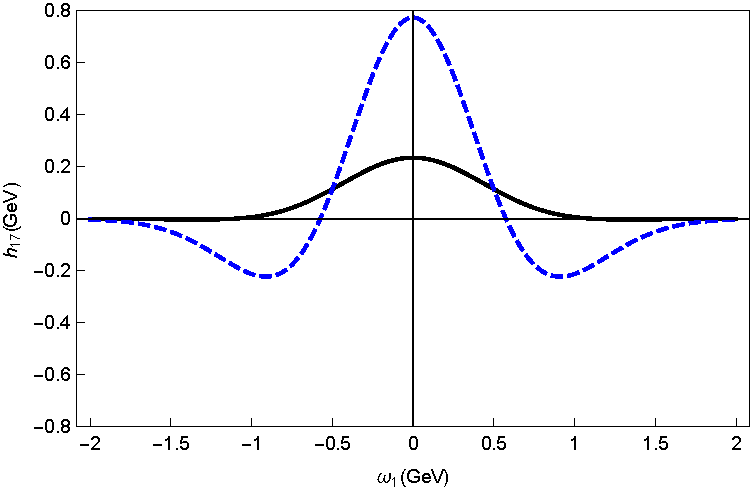
\includegraphics[scale=0.6]{FigureMoment2Low.pdf}
\hspace{1cm}
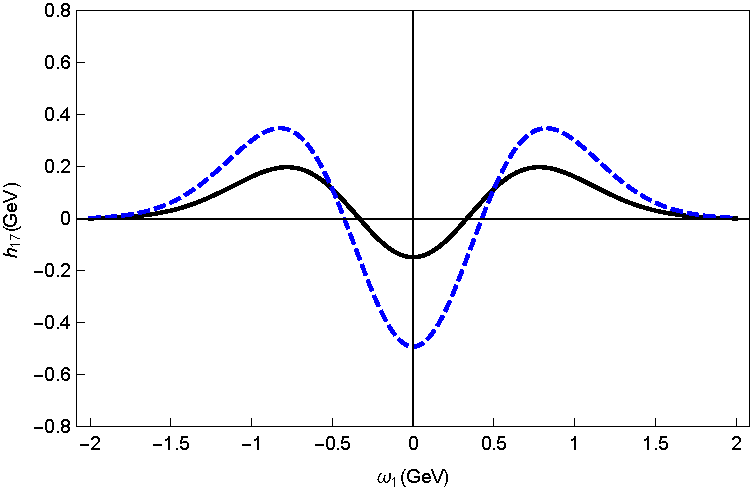
\includegraphics[scale=0.6]{FigureMoment2High.pdf}
\caption{\label{fig1} A comparison of the extremal models for $h_{17}$ as a sum of two lowest even Hermite polynomials times a Gaussian of width $0.5$ GeV used in \cite{Benzke:2010js} (dashed blue) to the same models allowed by current (2019) data (solid black). Left hand side:  The model with 2010 smallest possible second moment of $-0.31\mbox{ GeV}^4$ compared to 2019 smallest possible second moment of $0.03\mbox{ GeV}^4$. Right hand side:  The model with 2010 largest possible second moment of $0.49\mbox{ GeV}^4$ compared to 2019 largest possible second moment of $0.27\mbox{ GeV}^4$. 
}
\end{center}
\end{figure}
We define the mass split as $\Delta m_H=m_H^*-m_H$, where $m_H$ is a pseudo-scalar and $m_H^*$ is vector heavy meson containing a heavy quark of mass $m_Q$. 
At order $1/m_b$ the $\lambda_2=\Delta m_Hm_H/2$. We extractred the value of $\lambda_2$ using the isospin-averaged meson mass data \cite{Tanabashi:2018oca}. Following from this, we obtain $\lambda_2=0.119\pm 0.001\mbox{ GeV}^2$ for $B$ meson data. For the $D$ meson data we obtain $\lambda_2=0.13193\pm0.00002\mbox{ GeV}^2$ \cite{Gunawardana:2019gep}.\par
At order $\mathcal{O}(1/m_b^2)$ the expression for $\lambda_2$ is \cite{Gremm:1996df}
\begin{eqnarray}\label{eqn:chap5_l2_O_m_2}
\lambda_{2}\left(m_{b}\right)=\frac{\Delta m_{B} m_{B}^{2}-\Delta m_{D} m_{D}^{2}}{2\left(m_{B}-\kappa\left(m_{c}\right) m_{D}\right)}
\end{eqnarray} 
Equation (\ref{eqn:chap5_l2_O_m_2}) provides $\lambda_2=0.112\pm 0.001\mbox{ GeV}^2$. In comparison, $\mu_G^2/3=0.118\pm 0.020\mbox{ GeV}^2$  \cite{Gambino:2016jkc} is equal to all these values of $\lambda_2$ within the error. As a result, it is currently not possible to distinguish between $\lambda_2$ and $\mu_G^2$. Hence, in the following work we use $\mu_G^2/3$ from \cite{Gambino:2016jkc}, and we assume a similar behavior for all other HQET parameters. This situation can be improved with the availability of the future Belle II data and Lattice QCD. These new data can improve the estimates of HQET parameters and the moments. 

\subsection{Resolved photon contributions for $Q^q_1-Q_{7\gamma}$}

In the following work, we will use the moments of subleading shape function to better constrain the resolved photon contributions from the $Q_1^q-Q_{7\gamma}$. As shown in \cite{Benzke:2010js} the contribution from $Q^u_1-Q_{7\gamma}$ vanishes. The contribution from $Q^c_1-Q_{7\gamma}$ is given by

\begin{equation}\label{F17def}
{\cal F}^{17}_E = \frac{C_1(\mu)}{C_{7\gamma}(\mu)}\,\frac{\Lambda_{17}(m_c^2/m_b,\mu)}{m_b},
\end{equation}
where the nonperturbative quantity $\Lambda_{17}$ is defined in equation (\ref{eqn:chapter3_soft_functions}), and it depends on non-local forward scattering matrix element $h_{17}$. Since the $h_{17}$ cannot be obtained from first principles, we use its moments to construct a phenomenological model to describe $h_{17}$. Using the general decomposition provided in sections \ref{sec:SI_mat_decomp}, \ref{sec:SD_mat_decomp} and the numerical estimates of HQET parameters found in \cite{Gambino:2016jkc} we construct new model to better constraint ${\cal F}^{17}_E$.\par
The $Q^q_1-Q_{7\gamma}$ part of the resolved photon contribution to the estimate of CP asymmetry is given in equation (\ref{eqn:resolved_p_cont_CP}). This contribution is defined by the nonperturbative parameters $\tilde{\Lambda}^u_{17}$ and $\tilde{\Lambda}^c_{17}$. With the new information on the moments of subleading shape function $h_{17}$ we would like to revisit the evaluation of these nonperturbative parameters. In addition, we consider the uncertainty generated in evaluation of charm and bottom quark masses.
\vspace{-0.3cm}
\subsubsection{Uncertainty due to the running quark masses}
\vspace{-0.2cm}
For the evaluation of CP averaged rate we use the $m_c = m_c(\mu)$ defined in the $\overline{\mbox{MS}}$ scheme with $\mu=1.5$ GeV. Whereas, the evaluation of CP asymmetry is carried out by using $m_c = m_c(\mu)$ defined in the $\overline{\mbox{MS}}$ scheme with $\mu=2.0$ GeV.\par
The running of the quark masses is given as \cite{Buras:1998raa}
\vspace{-0.4cm}
\begin{eqnarray}\label{eqn:chap5_running_mass}
m(\mu)=m\left(\mu_{0}\right)\left[\frac{\alpha_{s}(\mu)}{\alpha_{s}\left(\mu_{0}\right)}\right]^{\frac{\gamma_{m}^{(0)}}{2 \beta_{0}}}\left[1+\left(\frac{\gamma_{m}^{(1)}}{2 \beta_{0}}-\frac{\beta_{1} \gamma_{m}^{(0)}}{2 \beta_{0}^{2}}\right) \frac{\alpha_{s}(\mu)-\alpha_{s}\left(\mu_{0}\right)}{4 \pi}\right],
\end{eqnarray}

where $\alpha_s, v(\mu), \gamma_m^{0,1}$, and $ \beta_{0,1}$ are given by

\begin{eqnarray}
\alpha_{s}(\mu)=\frac{\alpha_{s}\left(M_{Z}\right)}{v(\mu)}\left[1-\frac{\beta_{1}}{\beta_{0}} \frac{\alpha_{s}\left(M_{Z}\right)}{4 \pi} \frac{\ln v(\mu)}{v(\mu)}\right],
\end{eqnarray}
and 
\begin{align}
&v(\mu)=1-\beta_{0} \frac{\alpha_{s}\left(M_{Z}\right)}{2 \pi} \ln \left(\frac{M_{Z}}{\mu}\right)\nonumber\\
&\gamma_{m}\left(\alpha_{s}\right)=\gamma_{m}^{(0)} \frac{\alpha_{s}}{4 \pi}+\gamma_{m}^{(1)}\left(\frac{\alpha_{s}}{4 \pi}\right)^{2}\nonumber\\
&\beta_{0,1}\left(\alpha_{s}\right)=a_{1} \frac{\alpha_{s}}{4 \pi}+a_{2}\left(\frac{\alpha_{s}}{4 \pi}\right)^{2}\nonumber \\ 
&\gamma_{m}^{(0)}=6 C_{F} \qquad \gamma_{m}^{(1)}=C_{F}\left(3 C_{F}+\frac{97}{3} N-\frac{10}{3} f\right)
\end{align}

$C_{F}=\frac{N^{2}-1}{2 N}$, where $N$ is the number of color charges, and $f$ is the number of effective flavors. In the 2019 update of the 2018 PDG listing we found $m_c(\,m_c)=1.27\pm0.02$ GeV \cite{Tanabashi:2018oca}. The coupling constant is given by $\alpha_s(\mu=m_c) = 0.38 \pm0.03$ \cite{Tanabashi:2018oca}. Using these values and equation (\ref{eqn:chap5_running_mass}) we obtain $m_c(1.5 \mbox{ GeV})=1.20\pm0.03$ GeV and $m_c(2.0 \mbox{ GeV})=1.10\pm0.03$ GeV.\par
In \cite{Benzke:2010js} the estimate of $\Lambda_{17}$ was obtained by using the $m_c = 1.131$ GeV. This charm quark mass is based on smaller vale of $m_c(m_c)$ \cite{Hoang:2005zw}, and it was used in \cite{Misiak:2006zs,Misiak:2006ab} as well. This change in the charm mass tends to slightly affect the estimates of $\Lambda_{17}, \tilde{\Lambda}_{17}^c$.\par
The mass of the bottom quark is obtained by using the shape function scheme \cite{Benzke:2010js,Bosch:2004th}. The updated HFLAG \cite{Amhis:2016xyh} value of $m_b$ is $4.58\pm0.03$ GeV. This value should be compared to the $m_b = 4.65$ GeV used in \cite{Benzke:2010js}.
\vspace{-0.3cm}
\subsubsection{$\Lambda_{17}$ estimates based on expanded penguin function}
\vspace{-0.2cm}
As shown in the equation (\ref{eqn:chapter3_soft_functions}), the soft function $h_{17}$, which appears in the expression of $\Lambda_{17}$, is convoluted with the penguin function ($F(x)$), where $F$ is defined in equation (\ref{eqn:chapter3_penguin_fn}). The expansion of the $1-F(x)$ is given in equation (\ref{eqn:chapter3_F_expansion}), which is obtained for $x>1/4$.\par
In the region $\omega_1\ll 4m^2_c/m_b\approx 1.2-1.3$ GeV we can expand the $F(x)$ and obtain the $\Lambda_{17}$ in terms of moments of the subleading shape function. Starting from the expression of $\Lambda_{17}$ \cite{Benzke:2010js}
\begin{eqnarray}\label{eqn:chap5_L17power}
   \Lambda_{17}\Big(\frac{m_c^2}{m_b},\mu\Big)
   &=& e_c\,\mbox{Re} \int_{-\infty}^{\bar\Lambda}\!d\omega
    \int_{-\infty}^\infty \frac{d\omega_1}{\omega_1} \nonumber\\
   &\quad\times& \left\{ \left( \frac{m_b+\omega}{m_b} \right)^3 
    \left[ 1 - F\!\left( \frac{m_c^2-i\varepsilon}{(m_b+\omega)\,\omega_1} \right) \right]
    + \frac{m_b\,\omega_1}{12m_c^2} \right\} g_{17}(\omega,\omega_1,\mu) \,.
\end{eqnarray}
Using the definition of $h_{17}$ we have $\langle\omega^0\,\omega_1^k\,g_{17}\rangle=\langle\omega_1^k\,h_{17}\rangle$. Then the expansion of the penguin function provides \cite{Gunawardana:2019gep}:
\begin{equation}\label{eqn:chap5_Lambda17expanded}
\Lambda_{17}^{\mbox{\scriptsize expanded}}=  -\dfrac{e_c m_b^3}{560\,m_c^6} \langle\omega^0\,\omega_1^2\,g_{17}\rangle+\cdots=-6\pm5\mbox{ MeV}+\cdots,
\end{equation}

where $\cdots$ denotes the contributions from the higher order moments over $\omega_1$. Traditionally, the contribution from the zeroth moment in $\omega_1$ is subtracted  in equations (\ref{eqn:chapter3_soft_functions}) and (\ref{eqn:chap5_L17power}), and its magnitude is $-e_cm_b2\lambda_2/(12m_c^2)=-42\pm7 \mbox{ MeV}$. The contributors to the uncertainty in the equation (\ref{eqn:chap5_Lambda17expanded}) are $\langle\omega^0\,\omega_1^2\,g_{17}\rangle$, $m_b$, and $m_c$. These uncertainties were added in quadrature.\par
In the past, the size of the contribution from higher operators was a concern for the authors in \cite{Voloshin:1996gw, Ligeti:1997tc, Grant:1997ec, Buchalla:1997ky}. They have noticed the numerical suppression arising from the expansion of the penguin function \cite{Gunawardana:2019gep}. They have noticed the numerical suppression arising from the expansion
of the penguin function, but the lack of knowledge of the matrix elements prevented
them from making conclusive statements.\par
The first term in the equation (\ref{eqn:chapter3_F_expansion}) is suppressed by a factor $\sim 50$ compared to the third term. However, when the third term is combined with the second moment, we obtain  $-6\mbox{ MeV}$. This is only suppressed by a factor of $7$ compared to the zeroth moment. This smaller suppression is consistent with the power counting of $m_c^2\sim m_b\Lambda_{\mbox{\scriptsize QCD}}$, which disfavors the expansion of the penguin function \cite{Gunawardana:2019gep}.\par
Consider the $1/m^n_b$ corrections to $\Lambda_{17}^{\mbox{\scriptsize expanded}}$, which are obtained by expansion of $F(x)$ in $\omega/m_b$. By definition, $\Lambda_{17}^{\mbox{\scriptsize expanded}}=\delta \Lambda_{17}^{(0)}$. For $\delta\Lambda_{17}^{(1)}$ we have  \cite{Gunawardana:2019gep}:

\begin{eqnarray}\label{eqn:chapter5_dLamda_17_1}
\delta \Lambda_{17}^{(1)}&=& -\dfrac{e_c}{3\,m_c^2} \langle\omega^1\,\omega_1^0\,g_{17}\rangle-\dfrac{e_cm_b}{18\,m_c^4} \langle\omega^1\,\omega_1^1\,g_{17}\rangle-\dfrac{3e_cm_b^2}{280\,m_c^6} \langle\omega^1\,\omega_1^2\,g_{17}\rangle+\cdots\nonumber\\
&=&\left(-9\pm5\mbox{ MeV}\right)+\left(-6\pm5\mbox{ MeV}\right)+\left(-1\pm1\mbox{ MeV}\right)+\cdots=-16\pm7\mbox{ MeV}+\cdots\,.\nonumber\\ 
\end{eqnarray}

Again in the equation (\ref{eqn:chapter5_dLamda_17_1}), we observe a slow convergence. Only in the third term we see a suppression compared to the first two terms. Although $\delta \Lambda_{17}^{(1)}$ is a $\Lambda_{\mbox{\scriptsize QCD}}/m_b$ correction, equation (\ref{eqn:chapter5_dLamda_17_1}) indicates that the $\delta \Lambda_{17}^{(1)}$ is comparable in size to $\Lambda_{17}^{\mbox{\scriptsize expanded}}$. Even if we add the contribution of $\langle\omega^0\,\omega_1^0\,g_{17}\rangle$ to $\Lambda_{17}^{\mbox{\scriptsize expanded}}$, $\delta \Lambda_{17}^{(1)}$ is only suppressed by a factor of  three \cite{Gunawardana:2019gep}.\par  
The $\Lambda^2_{\mbox{\scriptsize QCD}}/m^2_b$ correction to the $\Lambda_{17}^{\mbox{\scriptsize expanded}}$ is given by
\begin{eqnarray}
\delta \Lambda_{17}^{(2)}&=& -\dfrac{e_c}{2\,m_b\,m_c^2} \langle\omega^2\,\omega_1^0\,g_{17}\rangle-\dfrac{e_c}{9\,m_c^4} \langle\omega^2\,\omega_1^1\,g_{17}\rangle+\cdots\nonumber\\
&=&\left(-0.8\pm1.1\mbox{ MeV}\right)+\left(1.2\pm0.6\mbox{ GeV}\right)+\cdots=0.4\pm1.3\mbox{ MeV}+\cdots\,.
\end{eqnarray}

The convergence generated by the expansion of $F(x)$ is again provide a slow convergence in the series. Finally, the $\Lambda^3_{\mbox{\scriptsize QCD}}/m^3_b$ correction for  $\Lambda_{17}^{\mbox{\scriptsize expanded}}$ is given by 
\begin{eqnarray}
\delta \Lambda_{17}^{(3)}&=& -\dfrac{e_c}{3\,m_b^2\,m_c^2} \langle\omega^3\,\omega_1^0\,g_{17}\rangle=-0.06\pm0.08\mbox{ MeV}+\cdots\,.
\end{eqnarray}\
As we expected, the $\delta \Lambda_{17}^{(3)}$ is order of magnitude smaller than the $\delta \Lambda_{17}^{(2)}$ correction.\par
The $\Lambda_{\mbox{\scriptsize QCD}}/m_b$ expansion for $\delta \Lambda_{17}$ works well with the exception of the first term. We speculate that this is due to the vanishing of $\langle\omega^0\,\omega_1^1\,g_{17}\rangle$, which makes the zeroth term in the expansion $\Lambda_{17}$ given in equation (\ref{eqn:chap5_L17power}) smaller than it ``should" be. Since in general for $l>0$ the moments $\langle\omega^l\,\omega_1^k\,g_{17}\rangle$ do not vanish, there is no such suppression beyond the zeroth term \cite{Gunawardana:2019gep}. Altogether we find $\Lambda_{17}^{\mbox{\scriptsize expanded}}+\delta \Lambda_{17}^{(1)}+\delta \Lambda_{17}^{(2)}+\delta \Lambda_{17}^{(3)}=-22\pm9\mbox{ MeV}$, where the uncertainties were added in quadrature.\par
Since the assumtons on the support of $h_{17}$ and resulting
expansion of the penguin function are too restrictive \cite{Benzke:2010js, Gunawardana:2019gep}, we will turn to a different approach to analyze the $\Lambda_{17}$.

\section{Modeling of $h_{17}$}\label{Model}

The $h_{17}$ is an even function, and it has a dimension of mass and in the heavy quark limit. As shown in the section \ref{Q1Q7_contr}, the $\omega_1$ is defined in the domain of $-\infty\leq\omega_1\leq \infty$. For the modeling of $h_{17}$ it is beneficial to have a systematic
expansion of $h_{17}$, e.g. in terms of a complete orthonormal set of basis functions \cite{Gunawardana:2019gep}. In \cite{Ligeti:2008ac} such a expansion was suggested to describe the leading order shape function. In our work we use an expansion in terms of Hermite polynomials multiplied by a Gaussian of width $\sigma$ \cite{Gunawardana:2019gep}:

\begin{equation}\label{h17General} 
h_{17}(\omega_1,\mu)=\sum_n a_{2n} H_{2n}\left(\frac{\omega_1}{\sqrt{2}\sigma}\right)e^{-\frac{\omega_1^2}{2\sigma^2}},
\end{equation}

where $H_{2n}$ are even Hermite polynomials, and the coefficients $a_{2n}$ are related to the moments of the $h_{17}$. In the following we refer to these models by the numbers of Hermite polynomials they contain. It is important to note that the  $2k$-th moment of $h_{17}$ only depends on the coefficients $a_{2n}$ with $n\leq k$, for a given value of $\sigma$. This is due to the orthogonality between Hermite polynomials. For instance, the zeroth moment of $h_{17}$ only depends on $a_0$ and the second moment of $h_{17}$ only depends on $a_0$ and $a_2$. As a result, we use the first $2k$-th moments to determine $a_{2n}$ with $n\leq k$. Using $\langle\omega^0\,\omega_1^k\,g_{17}\rangle=\langle\omega_1^k\,h_{17}\rangle$ we obtain  $a_0$ and $a_2$ \cite{Gunawardana:2019gep}:

\begin{equation}\label{a0a2}
a_0=\frac{\langle\omega_1^0\,h_{17}\rangle}{\sqrt{2\pi}|\sigma|}, \qquad a_2=\frac{\langle\omega_1^2\,h_{17}\rangle-\sigma^2\langle\omega_1^0\,h_{17}\rangle}{4\sqrt{2\pi}|\sigma|^3}.
\end{equation}

Since the $h_{17}$ is a soft function, it can be further constrained by using $|h_{17}(\omega_1,\mu)|\leq$ 1 GeV. as in \cite{Benzke:2010js}, that it should not have any significant structures, such as peaks or zeros, outside the range $|\omega_1|\leq 1$ GeV. This allows us to restrict the range of $\sigma$. For example, assuming a model of a sum of two Hermite polynomials, for given values of $\langle\omega_1^0\,h_{17}\rangle$ and $\langle\omega_1^2\,h_{17}\rangle$, the requirement on significant structures only for $|\omega_1|\leq 1$ GeV gives an upper bound on $\sigma$ and the condition $|h_{17}(\omega_1,\mu)|\leq$ 1 GeV gives a lower bound on $\sigma$. For example, assuming the central values for  $\langle\omega_1^0\,h_{17}\rangle=0.237 \mbox{ GeV}^2$ and $\langle\omega_1^2\,h_{17}\rangle=0.15\mbox{ GeV}^4$ gives $0.27\mbox{ GeV}<\sigma<0.62\mbox{ GeV}$. For other values of $\langle\omega_1^0\,h_{17}\rangle$ and   $\langle\omega_1^2\,h_{17}\rangle$ within their one standard deviation range, the range of $\sigma$ can be larger, but we restrict $\sigma$ to be less than 1 GeV. As we will see below, this does not affect our estimates in practice since the extremal values we obtain are for $\sigma<$ 1 GeV anyway \cite{Gunawardana:2019gep}.\par
In the following, we consider models up to and including four Hermite polynomials. The models with one and two hermite polynomials are defined using known moments. However, models with three and four Hermite polynomials are defined with unknown moments. 

\subsection{One Hermite polynomial model }

The $\sigma$ is not defined by the moments of $h_{17}$. As a result, we use both zero and second moments to fix the value of $\sigma$ in one Hermite polynomial model. Following from this, we define the one Hermite polynomial model 

\begin{equation}
h^{\mbox{\scriptsize model-1}}_{17}(\omega_1)=\frac{\langle\omega_1^0\,h_{17}\rangle}{\sqrt{2\pi}|\sigma|}e^{-\frac{\omega_1^2}{2\sigma^2}}.
\end{equation}

The second moment of $h^{\mbox{\scriptsize model-1}}_{17}$ implies $\sigma=\sqrt{\langle\omega_1^2\,h_{17}\rangle/\langle\omega_1^0\,h_{17}\rangle}$. This is also the condition for $a_2=0$ in (\ref{a0a2}) \cite{Gunawardana:2019gep}.\par
When we fix the value of the second moment to $\langle\omega_1^2\,h_{17}\rangle=0.27\mbox{ GeV}^4$, the $\sigma$ exceeds $1$ GeV for almost all the values of $\langle\omega_1^0\,h_{17}\rangle$ within its one standard deviation range. Based on the above constrains we reject such models. Even if we include these models we obtain $\Lambda_{17},\tilde\Lambda_{17}^u$, and $\tilde\Lambda_{17}^c$ that are included in the ranges for the two Hermite polynomials model below. The one Hermite polynomial model provides $\Lambda_{17}\in[-8,-1]$ MeV, $\tilde\Lambda_{17}^c\in[0,7.5]$ MeV, and $\tilde\Lambda_{17}^u\in[45,220]$ MeV \cite{Gunawardana:2019gep}.\par

\subsection{Sum of two Hermite polynomial model}

Including the zeroth and second moments of $h_{17}$ we construct the two Hermite polynomial model. The corresponding coefficients $a_0$ and $a_2$ for a given $\sigma$ are provided in equation (\ref{a0a2}).\par
Numerically scanning over the one standard deviation range of the moments and  the possible values of $\sigma$ in increments of  $\delta\sigma=0.01$ GeV, and based on the restrictions above on $h_{17}$ gives $\Lambda_{17}\in[-21,-1]$~MeV. The lower value is obtained for  $\langle\omega_1^0\,h_{17}\rangle=0.197\mbox{ GeV}^2$, $\langle\omega_1^2\,h_{17}\rangle=0.27\mbox{ GeV}^4$, $\sigma=0.44$ GeV, $m_c=1.17$ GeV, and $m_b=4.61$ GeV. The upper value is obtained for $\langle\omega_1^0\,h_{17}\rangle=0.277\mbox{ GeV}^2$, $\langle\omega_1^2\,h_{17}\rangle=0.03\mbox{ GeV}^4$, $\sigma=0.14$ GeV, $m_c=1.23$ GeV, and $m_b=4.55$ GeV. Thus the extremal values are obtained for extremal values of the two moments, anti-correlated, and the extremal values of $m_c$ and $m_b$, anti-correlated \cite{Gunawardana:2019gep}.\par
The dependence on $m_b$ and $m_c$ can be illustrated as follows: consider the set $\langle\omega_1^0\,h_{17}\rangle=0.197\mbox{ GeV}^2$, $\langle\omega_1^2\,h_{17}\rangle=0.27\mbox{ GeV}^4$, $\sigma=0.44$ GeV that leads to $\Lambda_{17}=-21$ MeV. Changing $m_b=4.61$ to $m_b=4.55$ GeV  while keeping $m_c=1.17$ GeV changes $\Lambda_{17}$ by $+1$ MeV. Thus the dependance on the value of $m_b$ is rather mild.  Changing $m_c=1.17$ GeV to $m_c=1.23$ GeV while keeping $m_b=4.61$ GeV changes $\Lambda_{17}$ by $+6$ MeV. Thus the dependance on the value of $m_c$ is more pronounced \cite{Gunawardana:2019gep}.\par
Similarly, we find the values of $\tilde{\Lambda}^c_{17}$. We have $\tilde\Lambda_{17}^c\in[0,10]$~MeV. The lower value is obtained for  $\langle\omega_1^0\,h_{17}\rangle=0.277\mbox{ GeV}^2$, $\langle\omega_1^2\,h_{17}\rangle=0.03\mbox{ GeV}^4$, $\sigma=0.14$ GeV, $m_c=1.13$ GeV, and $m_b=4.55$ GeV. The upper value is obtained for $\langle\omega_1^0\,h_{17}\rangle=0.197\mbox{ GeV}^2$, $\langle\omega_1^2\,h_{17}\rangle=0.27\mbox{ GeV}^4$, $\sigma=0.58$ GeV, $m_c=1.07$ GeV, and $m_b=4.61$ GeV. Again the extremal values are obtained for extremal values of the two moments, anti-correlated, and the extremal values of $m_c$ and $m_b$, anti-correlated \cite{Gunawardana:2019gep}.\par 
Finally, we consider the $\tilde{\Lambda}^u_{17}$. Using the parameterization above we have the expression 
\begin{equation} 
\tilde\Lambda_{17}^u = \frac23\,h_{17}(0)=\dfrac{3\sigma^2\langle\omega_1^0\,h_{17}\rangle-\langle\omega_1^2\,h_{17}\rangle}{3\sqrt{2\pi}|\sigma|^3}.
 \end{equation}
Since both moments are positive within their one standard deviation range, we can easily make $h_{17}(0)$ negative by choosing a small value of $\sigma$. Thus the smallest value of  $h_{17}(0)$ based on  $|h_{17}(\omega_1,\mu)|\leq1$ GeV is $-1$ GeV. For example, for the central values of $\langle\omega_1^0\,h_{17}\rangle$ and $\langle\omega_1^2\,h_{17}\rangle$, the value of $\sigma=0.27$ GeV gives $h_{17}(0)=-1$ GeV. To make $h_{17}(0)$ reach its highest possible value, we can choose the smallest value of $\langle\omega_1^2\,h_{17}\rangle$, 0.03 GeV$^4$ and the largest value of  $\langle\omega_1^0\,h_{17}\rangle$, 0.277 GeV$^2$. The extremal value of  $h_{17}(0)=0.33$ GeV is obtained for $\sigma =\sqrt{\langle\omega_1^2\,h_{17}\rangle/\langle\omega_1^0\,h_{17}\rangle}=0.33$ GeV. Based on this we find that $\tilde\Lambda_{17}^u\in[-660,220]$ MeV \cite{Gunawardana:2019gep}. 

\subsection{Sum of three Hermite polynomial model}

The sum of three Hermite polynomial model is obtained by using the fourth moment of $h_{17}$. For a given value of $\sigma$ we find the coefficient $a_6$ as \cite{Gunawardana:2019gep}

\begin{equation}\label{a4}
a_4=\frac{\langle\omega_1^4\,h_{17}\rangle-6\sigma^2\langle\omega_1^2\,h_{17}\rangle+3\sigma^4\langle\omega_1^0\,h_{17}\rangle}{96\sqrt{2\pi}|\sigma|^5}.
\end{equation}

The fourth moment is currently unknown since it relates to dimension 9 HQET matrix elements. The impact of this moment can be assessed, however, by considering the conservative bound $\langle\omega_1^4\,h_{17}\rangle\in [-0.3,0.3]$ GeV$^6$. Note that this range covers all  the numerical values obtained in equation (\ref{eqn:chap5_moments_numerical}). The bounds on $\Lambda_{17}$, $\tilde{\Lambda}_{17}^c$ and $\tilde{\Lambda}_{17}^u$ were obtained by restrictions of the values, zeros, and extremal points of $h_{17}$ to be below 1 GeV \cite{Gunawardana:2019gep}.

Numerically scanning over the one standard deviation range of the known zero and second moments, the range $[-0.3,0.3]$ GeV$^6$ for the unknown fourth moment in increments of 0.05 GeV and  the possible values of $\sigma$ based on the restrictions above gives $\Lambda_{17}\in[-24,3]$~MeV. The lower value is obtained for  $\langle\omega_1^0\,h_{17}\rangle=0.277\mbox{ GeV}^2$, $\langle\omega_1^2\,h_{17}\rangle=0.27\mbox{ GeV}^4$, $\langle\omega_1^4\,h_{17}\rangle=0.3\mbox{ GeV}^6$, $\sigma=0.32$ GeV, $m_c=1.17$ GeV, and $m_b=4.61$ GeV. The upper value is obtained for $\langle\omega_1^0\,h_{17}\rangle=0.237\mbox{ GeV}^2$, $\langle\omega_1^2\,h_{17}\rangle=0.03\mbox{ GeV}^4$, $\langle\omega_1^4\,h_{17}\rangle=-0.1\mbox{ GeV}^6$, $\sigma=0.34$ GeV, $m_c=1.17$ GeV, and $m_b=4.61$ GeV. The obtained range is only slightly different from the two Hermite polynomial model and reflects our generous range for the unknown fourth moment. 

Similarly we find the range for $\tilde\Lambda_{17}^c$. The positive values are included in the range obtained for a sum of two Hermite polynomials. We also get negative values in the range $[-5.6,0]$ MeV. The smallest value is obtained for $\langle\omega_1^0\,h_{17}\rangle=0.277\mbox{ GeV}^2$, $\langle\omega_1^2\,h_{17}\rangle=0.03\mbox{ GeV}^4$, $\langle\omega_1^4\,h_{17}\rangle=-0.11\mbox{ GeV}^6$, $\sigma=0.34$ GeV, $m_c=1.07$ GeV, and $m_b=4.61$ GeV. 


Unlike the two Hermite polynomial model we can make $h_{17}(0)$ reach a value of  $1$ GeV.  For example, taking the central values of the zeroth and second moment $\langle\omega_1^0\,h_{17}\rangle=0.237\mbox{ GeV}^2$, $\langle\omega_1^2\,h_{17}\rangle=0.15\mbox{ GeV}^4$ we find that for $\langle\omega_1^4\,h_{17}\rangle=0.1\mbox{ GeV}^6$ and $\sigma=0.25$ GeV $h_{17}(0)=1$ GeV. This result is not surprising. The moments are global properties of the function and it is hard to restrict using them values of the function at a single point. We conclude that for this model $\tilde\Lambda_{17}^u$ can be as large as 660 MeV, which is the largest value possible under the condition $|h_{17}(\omega_1,\mu)|\leq1$ GeV \cite{Gunawardana:2019gep}. 

\subsection{Sum of four Hermite polynomials model} 

The four Hermite polynomial model is constructed by considering the conservative estimate of $[-0.3,0.3]$ GeV$^8$ for the sixth moment $\langle\omega_1^6\,h_{17}\rangle$. This moment is related to the coefficient of the sixth Hermite polynomial ($H_6$).\par
Scanning over the values of the fourth and sixth moment we find that the smallest value of $\Lambda_{17}$ is $-22$ MeV, i.e. in the range we obtained for three Hermite polynomials. The highest value we obtain is  $5$~MeV for $\langle\omega_1^0\,h_{17}\rangle=0.277\mbox{ GeV}^2$, $\langle\omega_1^2\,h_{17}\rangle=0.03\mbox{ GeV}^4$, $\langle\omega_1^4\,h_{17}\rangle=-0.1\mbox{ GeV}^6$, $\langle\omega_1^6\,h_{17}\rangle=-0.2\mbox{ GeV}^8$, $\sigma=0.29$ GeV, $m_c=1.17$ GeV, and $m_b=4.61$ GeV. This should be compared to the maximum value of $-1$ MeV and $3$ MeV for the two and three Hermite polynomial models, respectively.   

For $\tilde\Lambda_{17}^c$ we find positive values that are already included in the ranges of the two and three Hermite polynomial models above. The smallest negative value we find for $\tilde\Lambda_{17}^c$ is $-7$ MeV for $\langle\omega_1^0\,h_{17}\rangle=0.277\mbox{ GeV}^2$, $\langle\omega_1^2\,h_{17}\rangle=0.03\mbox{ GeV}^4$, $\langle\omega_1^4\,h_{17}\rangle=-0.1\mbox{ GeV}^6$, $\langle\omega_1^6\,h_{17}\rangle=-0.2\mbox{ GeV}^8$, $\sigma=0.29$ GeV, $m_c=1.07$ GeV, and $m_b=4.61$ GeV.


Since $\tilde\Lambda_{17}^u$ obtains its smallest and largest possible values for the two and three Hermite polynomial models, there is no need to check the effect of the four Hermite polynomials model \cite{Gunawardana:2019gep}.

\subsection{Sum of five and six Hermite polynomials model} 

Similarly, we can continue with five and six Hermite polynomial models. For this we assume $k$-th moment is in the range $[-0.3,0.3]$ GeV$^{\,k+2}$. Scanning over the ranges in increments of $0.1$ GeV$^{\,k+2}$ we find that there are no solutions that satisfy our requirements on $h_{17}(0)$. One reason is the fast growth of the value of $H_n(0)$. Thus the coefficient of $H_n(0)$ needs to be smaller to maintain $|h_{17}(0)|\leq 1$ GeV.

\subsubsection{Summary}\label{subsec:summary} 
\vspace{-0.3cm}
Using a two Hermite polynomial model we find $\Lambda_{17}\in[-21,-1]$~MeV, $\tilde\Lambda_{17}^c\in[0,10]$~MeV, and $\tilde\Lambda_{17}^u\in[-660,220]$ MeV. Using a three Hermite polynomial model we find $\Lambda_{17}\in[-24,3]$~MeV, where $\langle\omega_1^4\,h_{17}\rangle$ is assumed to be in the range $[-0.3,0.3]$ GeV$^6$. The range for $\tilde\Lambda_{17}^c$ is found as $ \tilde\Lambda_{17}^c\in[-5.6,0]$~MeV. Also, the larges value of $\tilde\Lambda_{17}^u$ is $660$ MeV, which is based on our assumptions for $h_{17}$. Using the four Hermite polynomial model with similar assumptions on the fourth and sixth moments changes the highest value of $\Lambda_{17}$ to 5 MeV and the lowest value of $\tilde\Lambda_{17}^c$ to $-7$ MeV.\par
Altogether, we find $\Lambda_{17}\in[-24,5]$~MeV, $\tilde\Lambda_{17}^c\in[-7,10]$~MeV, and $\tilde\Lambda_{17}^u\in[-660,660]$ MeV after rounding to the closes integer.

\subsection{Phenomenological estimates}\label{subsec:pheno}

The 2010 phenomenological estimates of $\mathcal{F}_E|_{17}$ were given in section \ref{sec:nonpert_contr}. Based on the new estimates of $\Lambda_{17},\tilde{\Lambda}_{17}^u$ and $\tilde{\Lambda}_{17}^c$ we update the results found in \cite{Benzke:2010js}  and \cite{Benzke:2010tq}.\par
The $Q_{1}^q-Q_{7\gamma}$ contribution to the total uncertainty was evaluated by using $C_{1}(\mu)=1.257,C_{7}(\mu)=-0.407$ (calculated at $\mu=1.5\text{ GeV}$) and $m_b=4.58\text{ GeV}$. This gives \cite{Gunawardana:2019gep, Gunawardana:2019mos}: 
\begin{eqnarray}
\left.\mathcal{F}_{E}\right|_{17} \in[-0.3,+1.6] \%
\end{eqnarray} 
This should be compared  to the range givn in equation (\ref{eqn:chapter3_error_est})\cite{Benzke:2010js}. 
The total uncertainty of the rate can be obtained by using $\left.\mathcal{F}_{E}\right|_{88} \in[-0.3,+1.9] \%$ \cite{Benzke:2010js} along with either $\left.\mathcal{F}_{E}\right|_{78} ^{\mathrm{VIA}} \in[-2.8,-0.3] \%$ or the new experimental value from PDG, $\left.\mathcal{F}_{E}\right|_{78} ^{\exp } \in[-1.4,+2] \%$, which was obtained in section \ref{subsec:F_88}. Scanning over various contributions give \cite{Gunawardana:2019gep, Gunawardana:2019mos}
\begin{eqnarray}
-3.4 \%<\mathcal{F}_{E}(\Delta)<+3.2 \% \quad(\text { using } \mathrm{VIA})
\end{eqnarray}
This new range should be compared with the 2010 range given in equation (\ref{Fcurrentexp}), and it implies a reduction to the total error by a third. In contrast, by using the experimental estimate the new range becomes  
\begin{eqnarray}
-2.0 \%<\mathcal{F}_{E}(\Delta)<+5.5 \%\quad \text{ using exp.}
\end{eqnarray}

Compared to the 2010 range given in equation (\ref{eqn:F78_using_exp}), the new estimate reduces the total error by a half \cite{Gunawardana:2019gep, Gunawardana:2019mos}.\par
Plugging in our new estimates for $\tilde{\Lambda}_{17}^u$ and $\tilde{\Lambda}_{17}^c$ found in the section \ref{sec:resolved_cp_A} to the following expression
\begin{eqnarray}
\mathcal{A}_{X_{s} \gamma}^{\mathrm{SM}}=\left(1.15 \times \frac{\tilde{\Lambda}_{17}^{u}-\tilde{\Lambda}_{17}^{c}}{300 \mathrm{MeV}}+0.71\right) \%
\end{eqnarray}
gives us $-1.9 \%<\mathcal{A}_{X_{s} \gamma}^{\mathrm{SM}}<3.3 \%$. This should be compared to the 2010 range $-0.6 \%<\mathcal{A}_{X_{s} \gamma}^{\mathrm{SM}}<2.8 \%$ in \cite{Benzke:2010tq}

	\chapter{New results : Semileptonic decays of heavy mesons with artificial neural networks }\label{ANN_paper}

The study of semileptonic decays is an important new physics probe. For example, the recent analysis of semileptonic $B$ decays provides an anomaly in measurement related by lepton universality requirements. The advent of higher precision data provides new opportunities to explore whether similar anomalies exist in semileptonic decays of charmed particles \cite{Ablikim:2018evp, Ablikim:2018frk, Yuan:2019zfo, Riggio:2017zwh}.\par
Accurate theoretical description on charmed semileptonic decays provides useful information to extract the CKM matrix elements. Specifically, the decays of charmed $D^0$, $D^+$, or $D_s$ mesons provide one of the simplest way to determine the magnitudes of quark mixing parameters \cite{Grant:2019yar}. To extract these CKM matrix elements we use the knowledge of matrix elements of quark currents that describe strong interaction effects. Following from this, we find accurate description of semileptonic transitions, which is also needed for improvement of our understanding of quark hadronization mechanisms in QCD \cite{Grant:2019yar}. The exclusive semileptonnic transition between two meson states makes it a suitable system to theoretically analyze matrix elements of flavor changing currents. These flavor changing currents are parameterized by momentum dependent form factors. These form factors describes the hadronic part of the decay amplitude given by \cite{Grant:2019yar}

\begin{equation}\label{DPseudoscalar}
\langle K(\pi) (p_{K(\pi)}) | \bar q \gamma_\mu c | D (p_D) \rangle = F_+(q^2) \left(P_\mu - \frac{m_D^2-m_{K(\pi)}^2}{q^2} q_\mu \right) +
 F_0(q^2) \frac{m_D^2-m_{K(\pi)}^2}{q^2} q_\mu \ ,
\end{equation}

where $P = p_D + p_{K(\pi)}$ and $q = p_D - p_{K(\pi)}$. The differential decay rates ($d\Gamma/dq^2$) provide the means to study these form factors. By neglecting the final state fermion mass we write the differential decay rate for the semileptonic decay $D \rightarrow K(\pi) \ell \nu_{\ell}$ as \cite{Grant:2019yar}:

\begin{equation}\label{DifDistr}
\frac{d\Gamma(D \to K(\pi) \ell \nu_\ell)}{dq^2} =
\frac{G^2_F \left|V_{cq}\right|^2}{24 \pi^3} \left|{\bf p}_{K(\pi)}\right|^3 \left|F_+(q^2)\right|^2, 
\end{equation}

where $\left|{\bf p}_{K(\pi)}\right|$ is the magnitude of the $K(\pi)$ 3-momentum vector in the $D$-meson rest frame. Equation (\ref{DifDistr}) implies that only the $F_+(q^2)$ contributes for the analysis.\par  
Accurate calculations of the non-perturbative form factors $F_{+/0}(q^2)$ in the whole momentum range are very challenging \cite{Grant:2019yar}. Currently, we do not have a complete description of these form factors. Only Lattice QCD (LQCD)\cite{Aoki:2019cca} and QCD sum rules (QCDSR) \cite{Khodjamirian:2009ys} provide a model independent description in a limited $q^2$ range. However, these calculations are still improving. \par
We use rather general arguments based on analyticity of $F_+(q^2)$ to put constraints on shape of the form factors. The $z$ expansion is one of the popular approaches that uses the analyticity requirement to derive constraints on form factors. Here we series expand the form factor at some point $t=q^2$. This series can be improved by employing a conformal transformation to the parameter $z$

\begin{equation}\label{Zexp}
z(q^2)=\frac{\sqrt{t_+-t_0}-\sqrt{t_+-q^2}}{\sqrt{t_+-t_0}+\sqrt{t_+-q^2}},
\end{equation}

where the transformation $z(q^2)$ maps the interval $-\infty < q^2 < t_+$ onto the line segment $-1<z<1$. $t_0$ is a free parameter that corresponds to the values of $q^2$ that maps onto $z=0$, and $t_{\pm}= (m_D\pm m_\pi)^2$ \cite{Grant:2019yar}. Then the form factor is expanded as 

\begin{equation}\label{FF_z}
F_+(q^2)  =  \frac{1}{\Phi(q^2, t_0)} \sum_{k=0}^\infty a_k(t_0) z^k(q^2,t_0),
\end{equation}

where $\Phi(q^2, t_0)$ is an arbitrary function that is analytic anywhere but the unitarity cut \cite{Grant:2019yar,Boyd:1994tt,Becher:2005bg}. If there are poles present in between $q^2=0$ and the beginning of the unitarity cut, then the function $\Phi(q^2, t_0)$ can be written as $\Phi(q^2, t_0) = P(q^2) \phi(q^2, t_0)$, where $P(q^2) = z(q^2, m_V^2)$. For example, in $B\to \pi$ transitions such a pole present at $m_V=m_{B^*}$ \cite{Ananthanarayan:2011uc,Grinstein:2015wqa}. For the $B\to \pi$ transitions the expansion in equation (\ref{FF_z}) is converging rapidly, so only a few terms in the expansion are really needed. Thus the results from LQCD and QCDSR can be used to constrain the coefficients 
$a_k$ to provide a model-independent parameterization of the form factor \cite{Grant:2019yar}.\par
Since the form factors cannot be obtained from the first principles, phenomenological parameterizations are used to describe them. The  ``simple pole" model is the common parameterization, where ``pole'' refers to the lowest mass vector resonance formed in the t-channel with quantum numbers of the quark current \cite{Grant:2019yar}. For instance, the $D^\star$ vector state with quantum numbers $1^{-}$ is the dominant pole in the $D\to \pi e \bar\nu_e$ decay. The simple pole model is given as follows \cite{Grant:2019yar}:

\begin{equation}\label{FF_Pole}
F_+^{\rm pole}(q^2) = \frac{F_+(0)}{1-{\hat q}^2},
\end{equation}

where $F_+(0)$ is the value of the form factor at zero momentum recoil that has to be fixed either from the lattice QCD or from other arguments, and $\hat{q}^2=q^2/m_{D^*}^2$. The $m_{D*}$ is often taken as a fit parameter. However, physical masses of the states $D^*(2010)$ (for $D\to \pi$ transition) or $D^*_s(2112)$ (for $D\to K$ transition) could be used as well. Using more effective poles we construct more complicated models \cite{Grant:2019yar}

%
\begin{equation}\label{FF_ManyPoles}
F_+(q^2)=\frac{F_+(0)}{(1-\alpha)}\frac{1}{1-q^2/m_V^2}+
\sum_{k=1}^N \frac{\rho _k}{1-\frac{1}{\gamma_k}\frac{q^2}{m_V^2}},
\end{equation}

where $\alpha$  provides the strength of the dominant pole, $\rho_k$ is the strength of the $k$th term in the expansion, and
$\gamma _k=m_{V_k}^2/m_V^2$, with $m_{V_k}$ are masses of the higher mass states with vector quantum numbers. We can improve the accuracy of a given model by considering more effective poles. For example, a popular model that is due to Becirevic and Kaidalov (BK)\cite{Becirevic:1999kt} is given as 

%
\begin{equation}\label{FF_BK}
F_+^{BK}(q^2)  =  \frac{F_+(0)}{(1-\hat{q}^2)(1-a_{BK}\hat{q}^2)},
\end{equation}
%
where $a_{BK}$ is a fit parameter. 
Note that this model is obtained for the $N=1$ truncation of the expansion in equation (\ref{FF_ManyPoles}). As shown in the simple pole model, a good fit to experimental distribution is obtained 
by considering $m_V$ as a fit parameter. Further extension to the BK model is obtained by Ball and Zwicky \cite{Ball:2004ye},
%
\begin{equation}\label{FF_BZ}
F_+^{BZ} (q^2) = \frac{F_+(0)}{1-\hat{q}^2} \left(1+\frac{r_{BZ}\hat{q}^2}{1-a_{BZ}\hat{q}^2}\right),
\end{equation}
%
where $r_{BZ}$ and $a_{BZ}$ are the shape parameters.\par
In this work we are interested in learning whether choosing a specific functional form for the form factor induces a bias in the interpretation of an experimental analysis. This is analyzed in the machine learning (ML) approach. In particular, we are using the artificial neural networks (ANN) for this analysis. As shown in \cite{NNEstimator,NNEstimator2}, ANN can be used as an unbiased estimator of data. This fact has been used by the NNPDF collaboration to parameterize nucleon's parton distribution functions (PDF) \cite{Forte:2002fg,Ball:2014uwa,Rojo:2006nn}, and in form factor analysis of nucleon data \cite{Graczyk:2010gw,Alvarez-Ruso:2018rdx}.\par
In the following we build a statistical interpolating model based on ANNs, which contains information on experimental uncertainties and correlations. Nevertheless, ANN does not introduce theoretical bias. Following from \cite{Forte:2002fg,Ball:2014uwa}, we employ an approach based on multilayer feed-forward neural networks trained using the back-propagation learning algorithm \cite{Grant:2019yar}.

\section{Artificial Neural Networks}\label{ANN}
\subsection{Basic facts}

Recently, artificial neural networks are gaining traction in both academia and industry. As a result, ANN are widely used in experimental particle physics analysis. Specifically, the ANNs are extensively used in the jet finding algorithms \cite{Carleo:2019ptp}. A neural network can be thought of as a nonlinear function that connects the input and output data. In \cite{Grant:2019yar}, we explored another feature of ANNs, which is their ability to provide unbiased universal approximants to incomplete data \cite{NNEstimator,NNEstimator2}
%
\begin{center}
\begin{figure}[H]
\center
\includegraphics[scale=0.9]{Fig1.eps}
\caption{Structure of an artificial neural network with two hidden layers \cite{Grant:2019yar}. \label{Fig:ANN}}
\end{figure}
\end{center}
%
ANN mimic the structure of human neurons and consists of a set of interconnected units (see Figure.~\ref{Fig:ANN}) called {\it neurons} or {\it nodes}\cite{Grant:2019yar}. The activation state of a neuron is determined by the activation function ($g(x)$), which is determined by the activation status of the $i$ neurons connected to it. Each pair of these neurons is connected by a synapsis, which is  characterized by a weight $\omega_i$. Also, we add a threshold $\theta_i$ to control the activation state (``fire'') of neurons. In ANNs we categorize groups of neurons into layers. The first layer is called as input layer, which is associated with the input information. In the following work we used the value of $q^2$ for each bin in $q^2$ distribution of the CKM matrix element times the semileptonic form factor ($V_{cd}F_+(q^2)$) \cite{Grant:2019yar}. Furthermore, We used two nodes in the input layer, which improved the stability and the efficiency of the ANN. In section \ref{sec:feature_eng}, we provide further information on the input nodes. The final layer of the ANN is the output layer. The output layer provides fit for the $V_{cd}F_+(q^2)$ data along with its uncertainty. Conventionally, the layers between input and output layers are known as \textit{hidden layers}. Our ANN employs two hidden layers. Each of these hidden layers contain hundred nodes as well. 

\subsection{Forward propagation}
In the ANN training process we incrementally update the weights and thresholds so that they obtain optimal set of $\omega_i$ and $\theta_i$. This is achieved by minimizing the error function,
%
\begin{eqnarray}\label{error_fun}
E[{\omega,\theta}]\equiv\frac{1}{2}\sum_{A=1}^{n_p}
(o(q^2_{A})-y_{A})^2\,,
\end{eqnarray}
%
where $n_p$ is the number of pseudo-data used to train an ANN, $o( q^2_{A})$ is the output, which is given by the ANN's fit for a given input data $q^2_{A}$.
Here the target data point $y_A$, is obtained from the magnitude of the CKM matrix element times the semileptonic form factor, $\left|V_{cd} F_+(q^2)\right|$.
Note that the differential distribution of Eq.~(\ref{DifDistr}) is proportional to $\left|V_{cd} F_+(q^2)\right|^2$.
The $o(q^2_{A})$ is obtained using forward propagation. In order to achieve this we pass the input through a network of hidden nodes. The output from the first hidden layer with 
$n_1$ number of nodes is \cite{Grant:2019yar}
%
\begin{eqnarray}\label{first_layer_output}
\xi^{[1]}=g\left(\sum_{i=1}^{n_1}\omega_{i}^{[1]}q^2-\theta^{[1]}\right).
\end{eqnarray}
%
In this equation the response of each neuron is given by \cite{Grant:2019yar}
%
\begin{eqnarray}\label{sigmoid}
g(x)\equiv\frac{1}{1+e^{-x}},
\end{eqnarray}
% 
which is the \textit{sigmoid} activation function, and the summation over the $q^2$ data points is implied.
The $\xi^{[1]}$ is then used as an input for the second hidden layer with $n_2$ number of hidden nodes, and so on. The process is continued until the output layer of ANN is reached. In general, 
we can construct the output from $\ell$th hidden layer with $n_\ell$ number of nodes as \cite{Grant:2019yar}
%
\begin{eqnarray}\label{general_output}
\xi^{[\ell]}=g\left(\sum_{i=1}^{n_{\ell}}\omega_{i}^{[\ell]}\xi^{[\ell-1]}- \theta^{[\ell]} \right)  .
\end{eqnarray}
%
where $\xi^{[\ell-1]}$ is the output from the $(\ell-1)$th layer. The fit of the $L$ layer ANN $o(q^2)$ is then defined as   
%
\begin{eqnarray}
o(q^2)=\xi^{[L]}.
\end{eqnarray}
%
As shown above, the error function needed to be minimized. The popular choice of minimization is the \textit{gradient descent} (GC). Instead, 
we decided to use the non-linear conjugate gradient (NLCG) method \cite{Nocedal:2000sp, CGmethod} to minimize equation (\ref{error_fun}). 
In each iteration the $\omega_i$ and the $\theta_i$ update as \cite{Grant:2019yar}
%
\begin{eqnarray}\label{steepest_descent}
\delta\omega^{[\ell]} &=& -\eta\frac{\partial
E}{\partial\omega^{[\ell]}}\,, \nonumber \\ \\ \nonumber
\delta\theta^{[\ell]} &=& - \eta\frac{\partial
E}{\partial\theta_{i}^{[\ell]}},
\end{eqnarray} 
%
%
where $\eta$ is the learning rate at a given iteration. The NLCG method employed here does not require a pre-defined learning rate. 
The learning rate is initially determined by using line search algorithms \cite{Nocedal:2000sp}, and then iteratively updated based on the gradients that are in a conjugate direction to original gradient used in the line search algorithm. As it turns out, the NLCG method converges much faster than steepest descent method for the fits employed in this in this work. For more details on the NLCG method, see Ref. \cite{CGmethod}. 


\subsection{Back propagation}
The gradients of the error function are obtained by using the method of back propagation \cite{Demuth:2014}. 
Back propagation can be thought of as a consecutive application of the chain rule. By applying the chain rule to the $L$th layer we find \cite{Grant:2019yar}
%
\begin{eqnarray}\label{back_prop_final_layer}
\Delta^{[L]}= g'(h^{[L]})[o(q^2)-y]
\end{eqnarray} 
%
where $g'(h^{[L]})$ is the derivative of the activation function with respect to $h^{[L]}$ and 
%
\begin{eqnarray}\label{h_of_L}
h^{[L]}=\sum_{i=1}^{n_{L-1}}\omega^{[L]}\xi_{i}^{[L-1]}-\theta^{[L]}
\end{eqnarray} 
%
The derivatives with respect to $\omega_i$ and $\theta_i$ for layer $L$ are given by \cite{Grant:2019yar}
\begin{eqnarray}\label{delta}
 \frac{\partial
E}{\partial\omega_{i}^{[L]}} &=&
\Delta^{[L]}\xi_i^{[L-1]};\qquad
i=1,\ldots,n_{L-1}\,, \nonumber \\ \frac{\partial
E}{\partial\theta_{i}^{[L]}} &=& -
\Delta^{[L]}.
\end{eqnarray}
%
The output of equation (\ref{back_prop_final_layer}) is used to obtain the derivatives of the $(L-1)$th layer, $\Delta_j^{[L-1]}$,
%
\begin{eqnarray}
\Delta_j^{[L-1]}=g'\l(h^{[L-1]})
\Delta_i^{[L]}\omega^{[L]}\,.
\end{eqnarray}
%
The procedure is repeated for the hidden layers to find derivatives of error function with respect to $\omega_i$ and $\theta_i$ in each layer \cite{Grant:2019yar}, 
%
\begin{eqnarray}\label{delta1}
 \frac{\partial
E}{\partial\omega_{ij}^{[\ell]}} &=&
\Delta_i^{[\ell]}\xi_j^{[\ell-1]};\qquad
i=1,\ldots,n_\ell,\quad j=1,\ldots,n_{\ell-1}\,, \nonumber \\ 
\frac{\partial E}{\partial\theta_{i}^{[\ell]}} &=& -
\Delta_i^{[\ell]},\qquad i=1,\ldots,n_\ell,
\end{eqnarray}
%
Using these we can obtain the numerical gradient of the error function and find the corrections to the weights and thresholds. 

\section{Neural network training}
\subsection{Preparation of the data set}
The neural network training is performed on the real and artificial (pseudo) data. The pseudo data is generated based on the information from experimental data. Here we used the uncorrelated data, correlated data, normalized data, or some combination of these data types. These pseudo data was generated by following the method provided in \cite{Rojo:2006nn}. The experimental data set that is required to generate the pseudo data were provided in \cite{Ablikim:2015ixa}.
This experimental data set contains both uncorrelated and correlated statistical and systematic uncertainties. Also, the data set is provided with correlation matrices. The artificial data is generated as \cite{Grant:2019yar}
%
\begin{equation} \label{PD}
\left|V_{cd} F_{+}(q^2)\right|^{\rm{(art)},(k)}_i = \left|V_{cd} F_{+}(q^2)\right|^{\rm (exp)}_i + r_{t,i}^{(k)}\sigma_{t,i} + \sum_{j=1}^{N_{\rm sys}}r_{{\rm sys},j}^{(k)}\sigma_{{\rm sys},ji} 
+ \sum_{m=1}^{N_{\rm stat}}r_{{\rm stat},m}^{(k)}\sigma_{{\rm stat},mi}
\end{equation}
%
where $i=1,...,N_{\rm data}$ is the number of experimental data entries, which is equal to the number of $q^2$ bins. The term $\left|V_{cd} F_{+}(q^2)\right|^{\rm (exp)}_i$ is the central value of the experimental data point for a given $q^2$. The last three terms in the right hand side of the equation (\ref{PD}) provide the variation in the pseudo data sample. These terms represent total uncorrelated, correlated systematic, and correlated statistical uncertainties respectively. Following from the \cite{Rojo:2006nn}, we use all these information to generate the pseudo data samples. Here each ``uncertainty term'' is multiplied by a Gaussian random number $r_{t,i}^{(k)}$, $r_{{\rm sys},j}^{(k)}$, or $r_{{\rm stat},m}^{(k)}$  \cite{Grant:2019yar}. These random numbers have the mean of zero, and their standard deviation is equal to the bin uncertainty provided in \cite{Ablikim:2015ixa}. The total uncorrelated uncertainty, $\sigma_{t,i}$, is defined as 
%
\begin{equation}
\sigma_{t,i} = \sum_{j=1}^{N_{u,sys}}\tilde{\sigma}_{{\rm sys},ji} + \sum_{m=1}^{N_{u,sys}}\tilde{\sigma}_{{\rm stat},mi}
\end{equation}
%
where the $\tilde{\sigma}_{{\rm sys},ji}$ is uncorrelated systematic uncertainty and $\tilde{\sigma}_{{\rm stat},mi}$ statistical uncertainty. In \cite{Ablikim:2015ixa} we find the correlation matrix elements, $\mbox{corr}(j,i)$ as 
%
\begin{equation}
\sigma_{j,i} = \sqrt{\tilde{\sigma}_i \tilde{\sigma}_j \ \mbox{corr}(j,i)},
\end{equation}
%
where $\tilde{\sigma}_i$ is the uncorrelated uncertainty in the $i$-th bin of data. The $q^2$ values were randomly generated with a flat prior across the entire $q^2$ bin. Thus, every value of $d\Gamma^{\rm (art)}/dq^2$ has a different $q^2$ input. 

\subsection{Feature engineering}\label{sec:feature_eng}

We divided the generated pseudo data into 100 batches (one batch per network). Each batch has an average $q^2$ and a standard deviation relating to the $q^2$ values, which are used to scale the each value of $q^2$ which we have generated. Using the scaled $q^2$ data as a secondary input is recommended to improve the stability and the 
performance of ANNs \cite{patro2015normalization}. In particular, data standardization is a popular data scaling choice, and it is defined as 
$\tilde{q}^2_{ i\rho} = \left(q^2_{i\rho} - \bar{q}^2_{\rho}\right)/\sigma_\rho$, where $\rho$ is the batch number and $i$ is a single $q^2$ value in the batch. With this transformed data, 
each of our ANNs has the structure (2, 100, 100, 1), as the two hidden layers, each with 100 nodes, provide the most efficient structure without compromising the performance or accuracy. 
With a higher number of nodes, the ANN's fit would be more accurate, but the training speed would also be reduced. This data transformation, along with the conjugate gradient method, 
provides the minimum of the error function at $100$ iterations. In contrast, steepest descent method with a constant learning rate provides a comparable result only at 20000 iterations \cite{Grant:2019yar}. 

\section{Form factor parameterization with neural networks}

The $2\times10^{6}$ data points were generated for each of the 14 $q^2$ bins. As shown above, this data set was divided to hundred subsets, and each of these subsets contains with 280,000 unique pseudo-data points. After training all networks individually, we found the average ANN curve, with uncertainty, at every calculated $q^2$ value. The differential decay rate, $d\Gamma/dq^2$, and the $\left|V_{cd} F_{+}(q^2)\right|$ curves are shown in Fig. \ref{fig:diffGamma} and Figure \ref{fig:VFwithModels} respectively.
Further results of the ANN training and relevant graphs are available at the URL \url{https://s.wayne.edu/hepmachinelearning/}.

%

\begin{figure}[H]
\begin{center}
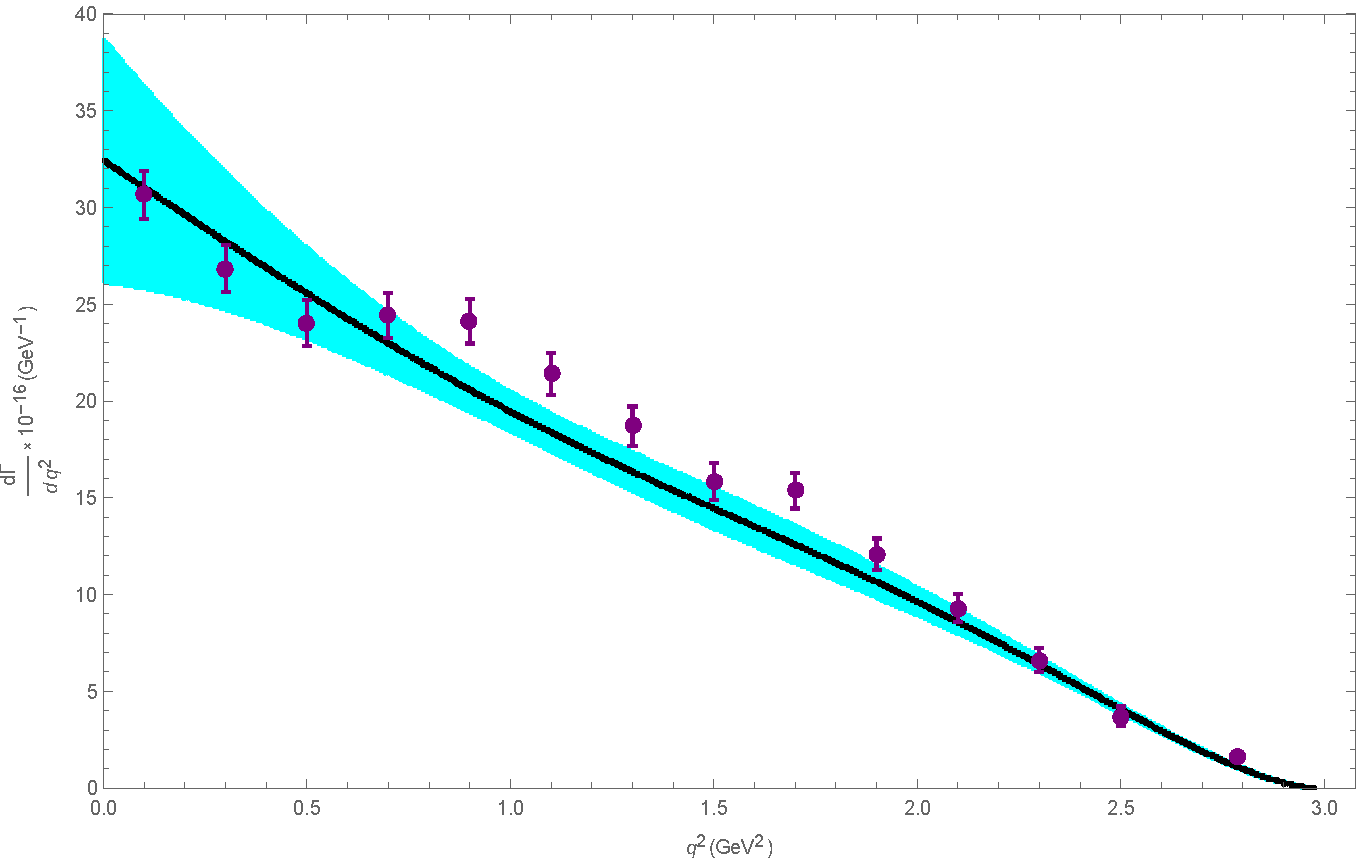
\includegraphics[scale=0.4]{FF exp final PDisVF_NN.pdf}
\caption{The averaged ANN result for the differential decay rate plotted against the experimental measurement \cite{Grant:2019yar}. The purple data points are the experimental data from \cite{Ablikim:2015ixa}. 
The black and cyan curves are the average value and one standard deviation, respectively, from the output of our averaged ANN .}
\label{fig:diffGamma}
\end{center}
\end{figure}
\vspace{-10mm}
In figure \ref{fig:VFwithModels} ANN fit is compared with some common form factor models: simple pole, the BK model (or modified pole), and the BZ model \cite{Becirevic:1999kt, Ball:2004ye} . 
%

\begin{figure}[H]
\begin{center}
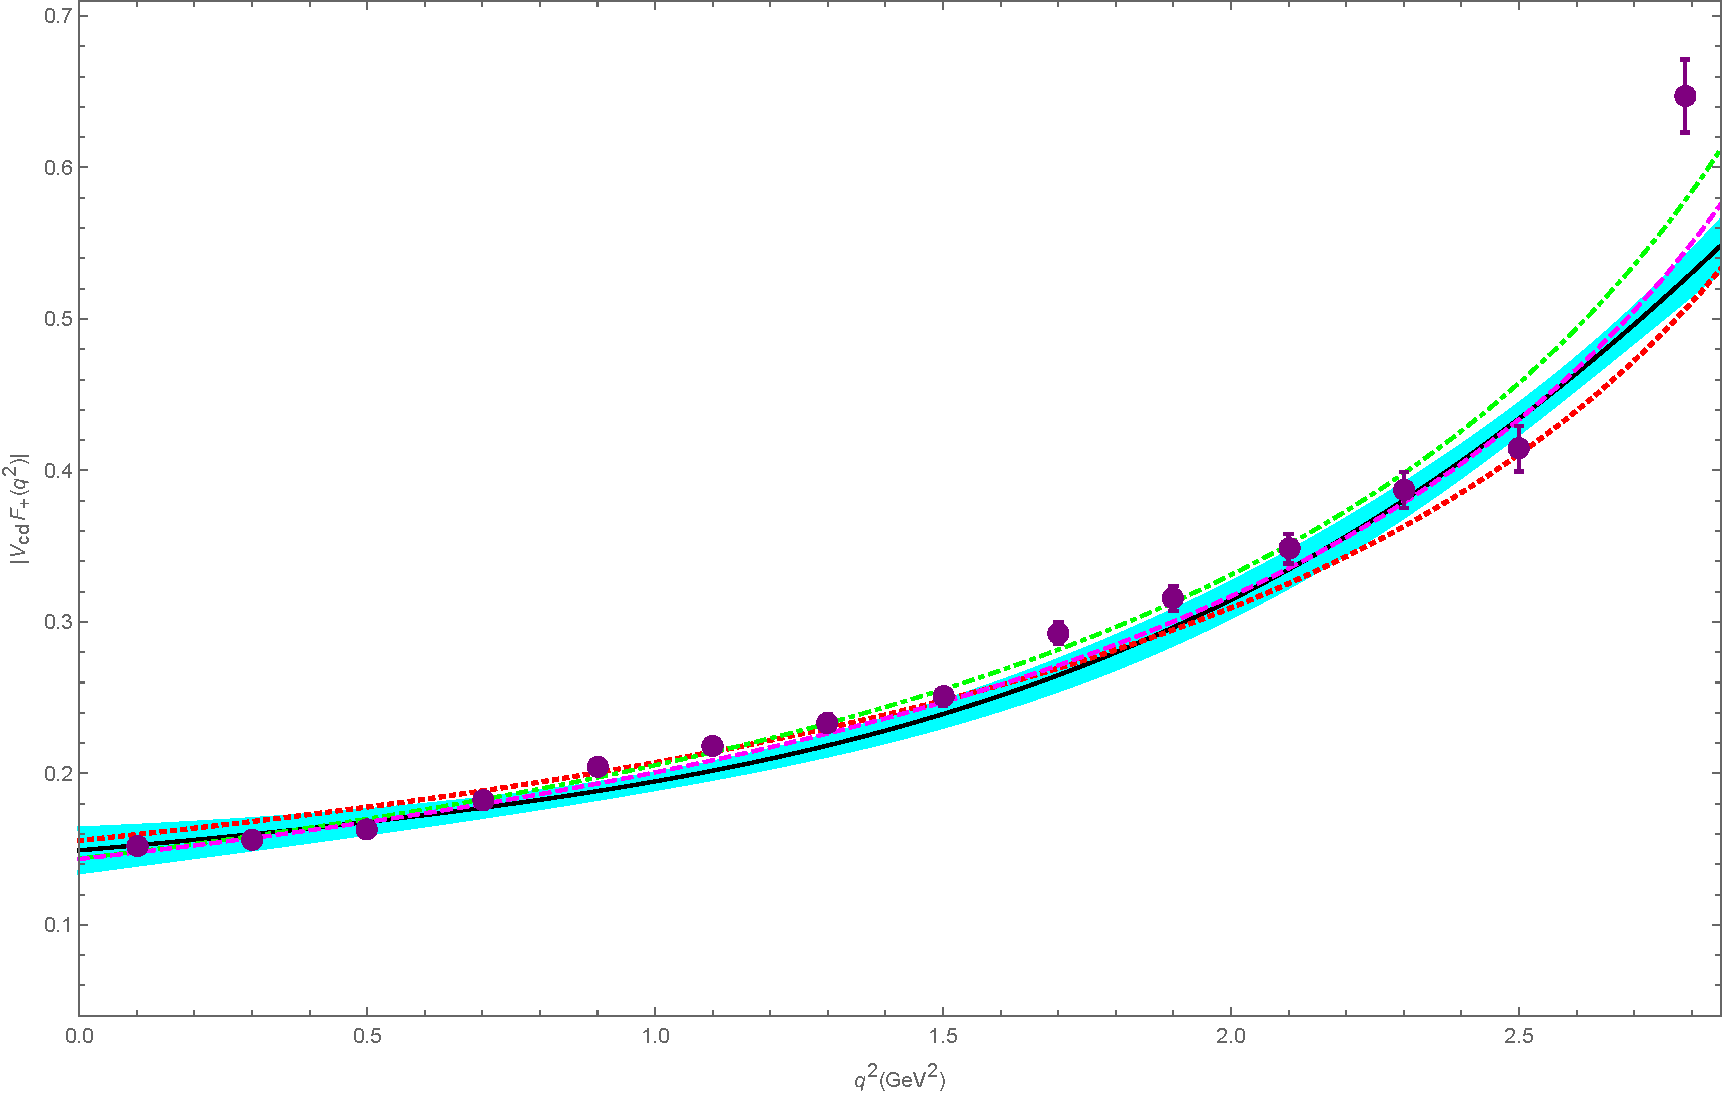
\includegraphics[scale=0.4]{FF exp final PDisVF_model.pdf}
\caption{ANN fits for $\left|V_{cd} F_+ (q^2)\right|$ plotted against the three models described in the text \cite{Grant:2019yar}. The black and cyan curves are the average value and one 
standard deviation, respectively, from the output of our neural network. The dotted red curve is the simple pole model. The dot-dashed green curve is the modified 
pole model. The dashed magenta curve is the BZ model. The purple data points are calculated from the experimental data in Ref \cite{Ablikim:2015ixa}.}
\label{fig:VFwithModels}
\end{center}
\end{figure}
\vspace{-8mm}
The $|V_{cd}F_+(0)|$ obtained from the model fits are roughly consistent with the ANN fit of the semileptonic decay data. 
%
	\chapter{Conclusion and future work}
\section{Conclusion}
Flavor physics is the study of different species of elementary particles \cite{flavor_phys}, and it provides tools to expand the boundaries of SM. For example, the radiative FCNC decay $\bar{B}\to X_s\gamma$ is considered as one of the standard candles of BSM \cite{Neubert:2005mu}. As another example, semileptonic decays of heavy mesons provide the means to extract the CKM matrix elements. Due to the effects of QCD, these decays are plagued with nonperturbative uncertainties. Therefore, it is important to control these uncertainties to the understand new physics in above processes. 
\par 
In this work we discussed the controlling the nonperturbative uncertainties in $\bar{B}\to X_s\gamma$ and semileptonic $D\to \pi l v$. In chapter \ref{chap:Matrix_elements}, we provided the construction of a new basis for the tensor decomposition of HQET and NRQCD matrix elements of any dimension. In chapter \ref{reevaluating_b_to_x}, we used the new basis for HQET/NRQCD to obtain the higher dimensional moments of subleading shape function. This function parameterizes the nonperturbative effects. We used these moments to model the subleading shape function and reevaluate the nonperturbative uncertainties. Finally, in chapter \ref{ANN_paper}, we used artificial neural networks to parameterize the shape of the form factor $F_+(q^2)$, which describes the nonperturbative effects of $D\to\pi l v$. 

\subsection{On HQET and NRQCD operators of dimension eight and above}
In chapter \ref{chap:Matrix_elements}, we provided the method to construct operators for the HQET and NRQCD Lagrangians at any given dimension. Although these theories employ different power counting schemes, the Lagrangians are closely related \cite{Manohar:1997qy}. We analyzed operators that contain two HQET fields or two NRQCD (NRQED) fields with an arbitrary number of covariant derivatives. These matrix elements can be written as nonperturbative HQET parameters multiplied by tensors constructed from the heavy quark velocity, the metric tensor, and the Levi-Civita tensor. We also use constraints
coming from the time-reversal (T) and parity (P) symmetries, hermitian conjugation, and the fact that we work in 3 + 1 dimension. At a given dimension, the number of allowed HQET operators are equivalent to the number of HQET parameters up to a possible color factor.\par
The new basis of HQET matrix elements allows us to easily determine the number of allowed HQET/NRQCD operators at a given dimension. This decomposition of matrix elements allows us to check whether given operators are linearly independent. The method also allows relating operators to one another easily. Following this, we constructed the HQET and
NRQCD Lagrangian at mass dimension 8 for the first time.\par
As shown in \cite{Kobach:2017xkw}, operators that contain symmetric product of two color matrices, such as  $\psi^\dagger E^i_aT^a  E^i_bT^b\psi$, can be decomposed in terms of a color octet and a color singlet operators, $\psi^\dagger E^i_a E^i_b\,d^{abc}T^c \psi$ and $\psi^\dagger E^i_a E^i_b \delta^{ab}\psi$. Since they only differ in their color structure, both will give the same linear combination of parameters.  Alternatively we can use the basis of  $\psi^\dagger E^i_a E^i_b\left\{T^a,T^b\right\}\psi$ and $\psi^\dagger E^i_a E^i_b \delta^{ab}\psi$. The operator $\psi^\dagger E^i_a E^i_b\left\{T^a,T^b\right\} \psi$ is generated by commutator and anti-commutators of covariant derivatives, and it is the only of the two that appears when calculating observables at tree level.  The operator $\psi^\dagger E^i_a E^i_b \delta^{ab}\psi$ will be generated when considering radiative corrections \cite{Manohar:1997qy}. For applications to inclusive $B$ decays, this operator arises only at order $\alpha_s/m^4_b$, beyond the current level of precision \cite{Gunawardana:2017zix}. Using the method presented above allows determining how many linearly independent operators there are for possible different color structures.\par
In section \ref{relating_with_lit}, we relate the HQET parameters of operators of dimension four, five, six, seven, and eight known from the literature to our basis. NRQCD operators up to dimension seven and NRQED operators up to dimension eight were previously known in the literature. We related these operators to the corresponding HQET matrix elements. The relation between the HQET/NRQCD operators and the matrix elements allows us to write the operators in terms of nonperturbative HQET parameters.\cite{Gunawardana:2017zix}.\par
In section \ref{applications}, we analyzed dimension nine spin-independent HQET parameters. Here we found 24 possible parameters (not including multiple color structures). Most importantly, we constructed the dimension eight NRQCD operators that do not appear in the $1/M^4$ NRQED Lagrangian. These allow presenting for the full $1/M^4$ bilinear NRQCD Lagrangian.\par
\subsection{Reevaluating the uncertainties in $\bar{B}\to X_s\gamma$ }
The section \ref{sec:chap5_moments_g_17} provides the moments of subleading shape function using data given in \cite{Gambino:2016jkc} and the basis developed in chapter \ref{chap:Matrix_elements} \cite{Gunawardana:2017zix}. This subleading shape function relates to the soft function $h_{17}$, which parameterize the nonperturbative uncertainty. The function $h_{17}$ defined in equation (\ref{eqn:chapetr3_h_17}), and it has the following properties: it is a real and even function over gluon momentum $\omega_1$, it's odd moments over $\omega_1$ vanish and it has dimensions of mass. Based on these properties we developed a new model for soft function $h_{17}$ based on a combination of \textit{Hermite polynomials} multiplied \textit{Gaussian}. The explicit form of the new model is given in section \ref{Model}.\par
The $h_{17}$ is is a soft function, so one expects it not to have significant structures beyond $\omega_1\leq 1$ GeV. This provides other constraints such as $\left|h_{17}\left(\omega_{1}\right)\right| \leq 1\mathrm{\, GeV}$, and it limits the function from having structures beyond $|\omega_1|\leq 1\text{ GeV}$. Scanning through different values of moments, we found a new estimate for $Q_1^q-Q_{7\gamma}$. Our estimate reduced the 2010 estimate \cite{Benzke:2010js} by a third. Also, we combined the new estimate for $Q_{7\gamma}-Q_{8g}$ with our new result for $Q_1^q-Q_{7\gamma}$ to obtain a new range for the total rate. Following from this we found that the uncertainty of the total rate is reduced by half compared to the 2010 values \cite{Benzke:2010js}.\par
The SM prediction for CP asymmetry is obtained by nonperturbative parameters $\tilde{\Lambda}_{17}^u$ and $\tilde{\Lambda}_{17}^c$. These parameters are also related to $h_{17}$. We reevaluated their ranges using our analysis. From this we found a new estimate for SM CP asymmetry as $-1.9 \%<\mathcal{A}_{X_{s} \gamma}^{\mathrm{SM}}<3.3 \%$, which is an increased range compared to the 2010 estimate \cite{Benzke:2010tq}. This is because of the increased range of the $\tilde{\Lambda}_{17}^u$.\par

\subsection{Semileptonic decays of heavy mesons with artificial neural networks}
The CKM matrix element $|V_{cd}|$ can be extracted most easily from semileptonic $D\rightarrow\pi l\nu$ decays. This decay is parameterized by the form factor $F_{+}(q^2)$, which describes the hadronic part of the decay amplitude. Experimentally, this form factor is studied by analyzing the differential decay rate of $d\Gamma/dq^2$. The lack of precise information about these form factors from the first principles of QCD is one of the main sources of uncertainties when extracting the CKM parameters. In spite of the recent progress from lattice QCD (LQCD), still, there is no ab-initio approach to describe the shape of the form factors in the whole physical region of momentum transfer $q^2$.\par
In view of the lack of first principle calculation for decay rates,  phenomenological parameterizations of form factors are used to model the shape. These models first estimate the hadronic form factor at one kinematic point and then extrapolate based on the assumed functional shape of the form factor. What systematic uncertainty does choosing a particular function brings to such extrapolation? To answer this question, we use machine learning (ML) framework. In section \ref{ANN}, we used artificial neural networks (ANN) as an unbiased estimator of data.\par 
We used an average of 100 feed-forward ANN with two hidden layers to obtain the unbiased estimate for $|V_{cd}|F_{+}(q^2)$. Each hidden layer contains 100 nodes \cite{Grant:2019yar}. The ANN performance was improved by using NLCG optimization method. We observed that NLCG method is 200 times faster compared to the common optimization methods such as gradient descent. The python code for ANN, results of the ANN training and relevant graphs are available at \url{https://s.wayne.edu/hepmachinelearning/}. The comparison between our ANN extrapolation of $|V_{cd}|F_{+}(q^2)$ against the existing models is provided in figure \ref{fig:VFwithModels}. From this we observe ANN fit is consistent with all the phenomenological models at low $q^2$ region. This implies that the ANN successfully extrapolated the $|V_{cd}|F_{+}(q^2)$ data to $q^2\to 0$.
 Most importantly, our ANN fit provides model independent parameterization of the $F_+(q^2)$ shape for the first time in literature. This was instrumental in developing the unitarity constraints on the form factor, which allowed for model-independent bounds on $V_{cd}$ \cite{Grant:2019yar}. 
\section{Future work}
We conclude with a remark on future developments. In section \ref{sec:gen_method}, we provided a general method of writing down all the possible HQET operators of any given dimension. It would be interesting to automatize the procedure using a computer program to construct these higher dimensional operators and the NRQCD Lagrangian. Also, certain multiple color structures were considered separately from the general method. It would be desirable to find a method that automatically generates these color structures.\par
We have not considered operators with more than two HQET or NRQCD (NRQED) fields. The one non-relativistic fermion sector can be combined with an additional non-relativistic field or an additional relativistic field.  Results for each case were presented in the literature  \cite{Bodwin:1994jh, Brambilla:2006ph, Brambilla:2008zg, Hill:2012rh, Dye:2016uep}, but not for an arbitrary operator dimension.\par
With the new information on the moments, we can better control the hadronic effects. However, the scale dependence on $1/m_b$ corrections is not fully controlled because, currently, we treat them at the leading order in $\alpha_s$. Therefore, to improve the $Q_{1}^q-Q_{7\gamma}$ contributions further, we need to take account of the $\alpha_s$ corrections.\par
Our model relies on the numerical estimates of the matrix elements of dimension eight operators. Still, it could further be improved if we knew the numerical estimates of dimension nine matrix elements. With the Belle II data, we can hope to have improvements on this.\par
In section \ref{sec:chap5_moments_g_17}, we only considered the quantities that are integrated over photon energy. The above moment information can be used to model $Q_{1}^q-Q_{7\gamma}$ contributions for quantities that are not integrated over photon spectrum.\par
The large amount of data that will be obtained at the B factory
Belle II will be ideal for deep learning. The extraction of CKM parameters using machine learning can be further improved with the new knowledge of optimization methods and deep learning. For example, our work provided in section \ref{ANN} uses the nonlinear conjugate methods (NLCG) to minimize the error function in the training process. The NLCG is a local optimizer. Whereas stochastic methods such as simulated annealing could have been more successful in optimizing the error function, and they are more suitable for deep learning. This is because these stochastic methods provide global optimization. With a large data set, we expect to develop deep neural networks utilizing parallel computation and graphical processing units.


%	
	
	% insert appendices
	% Comment the following line if you don't have an appendix
	% for a new appendix, copy appendices/appendix_a.tex and add a new line here
	%\begin{appendices}
\appendix
\addcontentsline{toc}{chapter}{Appendix A}
\appendix
\chapter*{Appendix A : Running of Wilson coefficients $C_1, C_7$ and $C_{8g}$}\label{app:Wilson}

The expressions for the running of Wilson coefficients $C_1, C_7$ and $C_{8g}$ are found in \cite{Buras:1998raa, Manohar:2000dt}.
\begin{eqnarray}
\begin{aligned} C_{j}^{(0)}\left(\mu_{b}\right) &=\sum_{i=1}^{8} k_{j i} \eta^{a_{i}} \quad(j=1, \ldots, 6) \\ C_{7 \gamma}^{(0) e f f}\left(\mu_{b}\right) &=\eta^{\frac{16}{23}} C_{7 \gamma}^{(0)}\left(\mu_{W}\right)+\frac{8}{3}\left(\eta^{\frac{14}{23}}-\eta^{\frac{16}{23}}\right) C_{8 G}^{(0)}\left(\mu_{W}\right)+C_{1}^{(0)}\left(\mu_{W}\right) \sum_{i=1}^{8} h_{i} \eta^{a_{i}} \\ C_{8 G}^{(0) e f f}\left(\mu_{b}\right) &=\eta^{\frac{14}{23}} C_{8 G}^{(0)}\left(\mu_{W}\right)+C_{1}^{(0)}\left(\mu_{W}\right) \sum_{i=1}^{8} \overline{h}_{i} \eta^{a_{i}} \end{aligned}
\end{eqnarray}
where
\begin{eqnarray}
\eta=\frac{\alpha_{s}\left(\mu_{W}\right)}{\alpha_{s}\left(\mu_{b}\right)}
\end{eqnarray}
To evaluate the Wilson coefficients at $\mu=1.5\text{ GeV}$ we use following boundary conditions \cite{Mohr:2015ccw, Tanabashi:2018oca}.
\begin{eqnarray}
\begin{aligned}
m_Z=(91.188\pm 0.002)\mbox{ GeV}\\
m_W=(80.379\pm 0.001)\mbox{ GeV}\\
\alpha_s(M_Z)=0.1181(1)\\
m_t^{\text{pole}}=172.9\pm0.4\mbox{ GeV}\\
m_b=4.18^{0.03}_{-0.02}\mbox{ GeV}
\end{aligned}
\end{eqnarray}
Note that the quark masses are given in pole mass scheme. However, pole masses of quarks can be converted into $\overline{\text{MS}}$ scheme as follows \cite{Tanabashi:2018oca}:
\begin{eqnarray}\label{polemss}
\overline{m}_{q}=m^{pole}_{q}\left(m^{pole}_{q}\right)\left(1-\frac{4 \alpha_{s}\left(m^{pole}_{q}\right)}{3 \pi}+\mathcal{O}\left(\alpha_{s}^{2}\right)\right)
\end{eqnarray}
The top quark mass obtained in equation (\ref{polemss}) is scaled down to $\mu=M_W$. Therefore, this gives us $m_t^{\overline{\text{MS}}}(\mu=M_W)=175.05\text{ GeV}$.\\
In addition, the $C_{7 \gamma}^{(0)}, C_{8 G}^{(0)}$ and $C_{1}^{(0)}$ are given by:
\begin{eqnarray}
\begin{array}{c}{C_{1}^{(0)}\left(\mu_{W}\right)=1} \\ {C_{7 \gamma}^{(0)}\left(\mu_{W}\right)=\frac{3 x_{t}^{3}-2 x_{t}^{2}}{4\left(x_{t}-1\right)^{4}} \ln x_{t}+\frac{-8 x_{t}^{3}-5 x_{t}^{2}+7 x_{t}}{24\left(x_{t}-1\right)^{3}} \equiv-\frac{1}{2} D_{0}^{\prime}\left(x_{t}\right)} \\ {C_{8 G}^{(0)}\left(\mu_{W}\right)=\frac{-3 x_{t}^{2}}{4\left(x_{t}-1\right)^{4}} \ln x_{t}+\frac{-x_{t}^{3}+5 x_{t}^{2}+2 x_{t}}{8\left(x_{t}-1\right)^{3}} \equiv-\frac{1}{2} E_{0}^{\prime}\left(x_{t}\right)}\end{array}
\end{eqnarray}
where $x_t=\frac{m_t^2}{M_W^2}$
Also, running of the $C_1$ is given by 
\begin{eqnarray}\label{c1new}
C_{1}^{(0)}(\mu)=\frac{1}{2} \eta^{-12 / 23}+\frac{1}{2} \eta^{6 / 23}
\end{eqnarray} 

\addcontentsline{toc}{chapter}{Appendix B}
\appendix
\chapter*{Appendix B : Useful identity}\label{appen_b}
The  Wilson line 
\begin{equation}
S_{\bar n}(x)=\mbox{\bf P}\exp \left( ig\int_{-\infty}^0 \,du \,\bar n\cdot A_s(x+u\bar n) \right)\,,
\end{equation}
obeys the equation $i\bar n\cdot D\,S_{\bar n}(x)=0$, where $iD^\mu=i\partial^\mu+gA^\mu$, see, e.g., \cite{Becher:2014oda} for a derivation.  Thus $i\bar n\cdot\partial S_{\bar n}(x)=-g\bar n\cdot A(x)S_{\bar n}(x)$. Taking the Hermitian conjugate of this identity gives $i\bar n\cdot\partial S^\dagger_{\bar n}(x)=S^\dagger_{\bar n}(x)g\bar n\cdot A(x)$. Consider now $i\bar n\cdot \partial \left(S_{\bar n}^\dagger(x) O(x) S_{\bar n}(x) \right)$, where $O(x)$ is an operator. Using the identities above we have 
\begin{eqnarray}
&&i\bar n\cdot \partial \left(S_{\bar n}^\dagger(x) O(x) S_{\bar n}(x) \right)=\nonumber\\
&=&\big(i\bar n\cdot \partial S_{\bar n}^\dagger(x)\big)O(x) S_{\bar n}(x) +S_{\bar n}^\dagger(x)\big(i\bar n\cdot \partial\, O(x)\big)S_{\bar n}(x) +S_{\bar n}^\dagger(x)O(x) \big(i\bar n\cdot \partial S_{\bar n}(x) \big)\nonumber\\
&=&S^\dagger_{\bar n}(x)g\bar n\cdot A(x)O(x) S_{\bar n}(x) +S_{\bar n}^\dagger(x)\big(i\bar n\cdot \partial\, O(x)\big)S_{\bar n}(x)-S_{\bar n}^\dagger(x) O(x) g\bar n\cdot A(x)S_{\bar n}(x)=\nonumber\\
&=& S^\dagger_{\bar n}(x)[g\bar n\cdot A(x),O(x)] S_{\bar n}(x)+S_{\bar n}^\dagger(x)\big[i\bar n\cdot \partial ,O(x)\big]S_{\bar n}(x)=S_{\bar n}^\dagger(x)\big[i\bar n\cdot D,O(x)\big]S_{\bar n}(x).
\end{eqnarray}
In the last line we have used the identity $\big[i\bar n\cdot \partial ,O(x)\big]f(x)=\big(i\bar n\cdot \partial\, O(x)\big)f(x)$ for an arbitrary function $f(x)$. Thus we have the identity 
 \begin{equation}
 i\bar n\cdot \partial \left(S_{\bar n}^\dagger(x) O(x) S_{\bar n}(x) \right)=S_{\bar n}^\dagger(x)\big[i\bar n\cdot D,O(x)\big]S_{\bar n}(x).
 \end{equation}
	%\end{appendices}
	
	
	\addcontentsline{toc}{chapter}{Bibliography}
  	\bibliographystyle{unsrt}
 	 \newpage

\begin{thebibliography}{99}

\vspace{0.5cm}

%\cite{Barger:1987nn}
\bibitem{Barger:1987nn} 
  V.~D.~Barger and R.~J.~N.~Phillips,
  \textit{Collider Physics},
   ADDISON-WESLEY 1987 

%\cite{Glashow:1961tr}
\bibitem{Glashow:1961tr} 
  S.~L.~Glashow,
  %``Partial Symmetries of Weak Interactions,''
  Nucl.\ Phys.\  {\bf 22}, 579 (1961).
  doi:10.1016/0029-5582(61)90469-2
  %%CITATION = doi:10.1016/0029-5582(61)90469-2;%%
  
%\cite{Weinberg:1967tq}
\bibitem{Weinberg:1967tq} 
  S.~Weinberg,
  %``A Model of Leptons,''
  Phys.\ Rev.\ Lett.\  {\bf 19}, 1264 (1967).
  doi:10.1103/PhysRevLett.19.1264
  %%CITATION = doi:10.1103/PhysRevLett.19.1264;%%
  
%\cite{SM_summary}
\bibitem{SM_summary} 
Wikipedia, URL: \url{https://commons.wikimedia.org/w/index.php?curid=4286964}


%\cite{Noether:1918zz}
\bibitem{Noether:1918zz} 
  E.~Noether,
  %``Invariant Variation Problems,''
  Gott.\ Nachr.\  {\bf 1918}, 235 (1918)
  [Transp.\ Theory Statist.\ Phys.\  {\bf 1}, 186 (1971)]
  doi:10.1080/00411457108231446
  [physics/0503066].
  %%CITATION = doi:10.1080/00411457108231446;%%  
  
%\cite{Griffiths:2008zz}
\bibitem{Griffiths:2008zz} 
  D.~Griffiths,
  \textit{Introduction to elementary particles},
  Wiley-VCH 2008  
      
  
%\cite{Lee:1956qn}
\bibitem{Lee:1956qn} 
  T.~D.~Lee and C.~N.~Yang,
  %``Question of Parity Conservation in Weak Interactions,''
  Phys.\ Rev.\  {\bf 104}, 254 (1956).
  doi:10.1103/PhysRev.104.254
  %%CITATION = doi:10.1103/PhysRev.104.254;%% 
  
%\cite{Peccei:1998jv}
\bibitem{Peccei:1998jv}
  R.~Peccei,
  %``Discrete and global symmetries in particle physics,''
  Lect.\ Notes Phys.\  \textbf{521}, 1-50 (1999)
  doi:10.1007/BFb010552
  [arXiv:hep-ph/9807516 [hep-ph]].
  %27 citations counted in INSPIRE as of 04 Apr 2020  
  
%\cite{Peskin:1995ev}
\bibitem{Peskin:1995ev} 
  M.~E.~Peskin and D.~V.~Schroeder,
  \textit{An Introduction to quantum field theory},
  Westviev Press 1995
  %%CITATION = INSPIRE-407703;%%      
  
%\cite{Yang:1954ek}
\bibitem{Yang:1954ek} 
  C.~N.~Yang and R.~L.~Mills,
  %``Conservation of Isotopic Spin and Isotopic Gauge Invariance,''
  Phys.\ Rev.\  {\bf 96}, 191 (1954).
  doi:10.1103/PhysRev.96.191
  %%CITATION = doi:10.1103/PhysRev.96.191;%% 
  
%\cite{Lancaster:2014pza}
\bibitem{Lancaster:2014pza} 
  T.~Lancaster and S.~J.~Blundell,
  \textit{Quantum Field Theory for the Gifted Amateur},
  Oxford University Press 2014
  %%CITATION = INSPIRE-1680925;%%  
  
  
%\cite{Manohar:2000dt}
\bibitem{Manohar:2000dt} 
  A.~V.~Manohar and M.~B.~Wise,
  %``Heavy quark physics,''
  Camb.\ Monogr.\ Part.\ Phys.\ Nucl.\ Phys.\ Cosmol.\  {\bf 10}, 1 (2000).
  %%CITATION = CMPCE,10,1;%%
  
  
%\cite{LlewellynSmith:1973yud}
\bibitem{LlewellynSmith:1973yud} 
  C.~H.~Llewellyn Smith,
  %``High-Energy Behavior and Gauge Symmetry,''
  Phys.\ Lett.\  {\bf 46B}, 233 (1973).
  doi:10.1016/0370-2693(73)90692-8
  %%CITATION = doi:10.1016/0370-2693(73)90692-8;%%  
  
\bibitem{Isidori:2010kg} 
  G.~Isidori, Y.~Nir and G.~Perez,
  %``Flavor Physics Constraints for Physics Beyond the Standard Model,''
  Ann.\ Rev.\ Nucl.\ Part.\ Sci.\  {\bf 60}, 355 (2010)
  doi:10.1146/annurev.nucl.012809.104534
  [arXiv:1002.0900 [hep-ph]].
  %%CITATION = doi:10.1146/annurev.nucl.012809.104534;%%
  
%\cite{Buras:1998raa}
\bibitem{Buras:1998raa} 
  A.~J.~Buras,
  %``Weak Hamiltonian, CP violation and rare decays,''
  hep-ph/9806471.
  %%CITATION = HEP-PH/9806471;%%  
  
%\cite{Chau:1984fp}
\bibitem{Chau:1984fp} 
  L.~L.~Chau and W.~Y.~Keung,
  %``Comments on the Parametrization of the Kobayashi-Maskawa Matrix,''
  Phys.\ Rev.\ Lett.\  {\bf 53}, 1802 (1984).
  doi:10.1103/PhysRevLett.53.1802
  %%CITATION = doi:10.1103/PhysRevLett.53.1802;%%  
  
%\cite{Wolfenstein:1983yz}
\bibitem{Wolfenstein:1983yz} 
  L.~Wolfenstein,
  %``Parametrization of the Kobayashi-Maskawa Matrix,''
  Phys.\ Rev.\ Lett.\  {\bf 51}, 1945 (1983).
  doi:10.1103/PhysRevLett.51.1945
  %%CITATION = doi:10.1103/PhysRevLett.51.1945;%% 
  
%\cite{Tanabashi:2018oca}
\bibitem{Tanabashi:2018oca} 
  M.~Tanabashi {\it et al.} [Particle Data Group],
  %``Review of Particle Physics,''
  Phys.\ Rev.\ D {\bf 98}, no. 3, 030001 (2018).
  doi:10.1103/PhysRevD.98.030001
  %%CITATION = doi:10.1103/PhysRevD.98.030001;%% 
  
%\cite{Buras:1994ec}
\bibitem{Buras:1994ec} 
  A.~J.~Buras, M.~E.~Lautenbacher and G.~Ostermaier,
  %``Waiting for the top quark mass, K+ ---> pi+ neutrino anti-neutrino, B(s)0 - anti-B(s)0 mixing and CP asymmetries in B decays,''
  Phys.\ Rev.\ D {\bf 50}, 3433 (1994)
  doi:10.1103/PhysRevD.50.3433
  [hep-ph/9403384].
  %%CITATION = doi:10.1103/PhysRevD.50.3433;%%    
  
%\cite{Jarlskog:1988ii}
\bibitem{Jarlskog:1988ii} 
  C.~Jarlskog and R.~Stora,
  %``Unitarity Polygons and CP Violation Areas and Phases in the Standard Electroweak Model,''
  Phys.\ Lett.\ B {\bf 208}, 268 (1988).
  doi:10.1016/0370-2693(88)90428-5
  %%CITATION = doi:10.1016/0370-2693(88)90428-5;%%  
  
%\cite{Glashow:1970gm}
\bibitem{Glashow:1970gm} 
  S.~L.~Glashow, J.~Iliopoulos and L.~Maiani,
  %``Weak Interactions with Lepton-Hadron Symmetry,''
  Phys.\ Rev.\ D {\bf 2}, 1285 (1970).
  doi:10.1103/PhysRevD.2.1285
  %%CITATION = doi:10.1103/PhysRevD.2.1285;%%  

%\cite{Gaillard:1974hs}
\bibitem{Gaillard:1974hs} 
  M.~K.~Gaillard and B.~W.~Lee,
  %``Rare Decay Modes of the K-Mesons in Gauge Theories,''
  Phys.\ Rev.\ D {\bf 10}, 897 (1974).
  doi:10.1103/PhysRevD.10.897
  %%CITATION = doi:10.1103/PhysRevD.10.897;%% 
  
%\cite{Ahmed:2012qqv}
\bibitem{Ahmed:2012qqv} 
  I.~Ahmed,
  %``Probing new physics through semileptonic flavor changing neutral current transition,''
  %%CITATION = INSPIRE-1478432;%%   
  
%\cite{Ellis:1977uk}
\bibitem{Ellis:1977uk} 
  J.~R.~Ellis, M.~K.~Gaillard, D.~V.~Nanopoulos and S.~Rudaz,
  %``The Phenomenology of the Next Left-Handed Quarks,''
  Nucl.\ Phys.\ B {\bf 131}, 285 (1977)
  Erratum: [Nucl.\ Phys.\ B {\bf 132}, 541 (1978)].
  doi:10.1016/0550-3213(77)90374-1
  %%CITATION = doi:10.1016/0550-3213(77)90374-1;%%  
  
%\cite{Shifman:1975tn}
\bibitem{Shifman:1975tn} 
  M.~A.~Shifman, A.~I.~Vainshtein and V.~I.~Zakharov,
  %``Light Quarks and the Origin of the Delta I = 1/2 Rule in the Nonleptonic Decays of Strange Particles,''
  Nucl.\ Phys.\ B {\bf 120}, 316 (1977).
  doi:10.1016/0550-3213(77)90046-3
  %%CITATION = doi:10.1016/0550-3213(77)90046-3;%% 

%\cite{Bander:1979px}
\bibitem{Bander:1979px} 
  M.~Bander, D.~Silverman and A.~Soni,
  %``CP Noninvariance in the Decays of Heavy Charged Quark Systems,''
  Phys.\ Rev.\ Lett.\  {\bf 43}, 242 (1979).
  doi:10.1103/PhysRevLett.43.242
  %%CITATION = doi:10.1103/PhysRevLett.43.242;%%   

%\cite{Misiak:2015xwa}
\bibitem{Misiak:2015xwa} 
  M.~Misiak {\it et al.},
  %``Updated NNLO QCD predictions for the weak radiative B-meson decays,''
  Phys.\ Rev.\ Lett.\  {\bf 114}, no. 22, 221801 (2015)
  doi:10.1103/PhysRevLett.114.221801
  [arXiv:1503.01789 [hep-ph]].
  %%CITATION = doi:10.1103/PhysRevLett.114.221801;%%  
  
%\cite{Lingel:1998fa}
\bibitem{Lingel:1998fa} 
  K.~Lingel, T.~Skwarnicki and J.~G.~Smith,
  %``Penguin decays of $B$ mesons,''
  Ann.\ Rev.\ Nucl.\ Part.\ Sci.\  {\bf 48}, 253 (1998)
  doi:10.1146/annurev.nucl.48.1.253
  [hep-ex/9804015].
  %%CITATION = doi:10.1146/annurev.nucl.48.1.253;%%   
  
%\cite{Grinstein:2017pvg}
\bibitem{Grinstein:2017pvg}
 B.~Grinstein,
 %``Lectures on Flavor Physics and CP Violation,''
 %doi:10.5170/CERN-2016-005.43
 [arXiv:1701.06916 [hep-ph]].
 
%\cite{Neubert:2005mu}
\bibitem{Neubert:2005mu} 
  M.~Neubert,
  %``Effective field theory and heavy quark physics,''
  doi:10.1142/9789812773579-0004
  hep-ph/0512222.
  %%CITATION = doi:10.1142/9789812773579_0004;%%  

%%%%%%%%%%%%%%%%%%%%%%%%%%%%%%%%%%%%%%%%%%%%%%%%%%%%%%%%%%%%%%%%%%%%%
%Chapter 2

%\cite{Petrov:2016azi}
\bibitem{Petrov:2016azi} 
  A.~A.~Petrov and A.~E.~Blechman,
  \textit{Effective Field Theories}, 
  World Scientific 2016
  %doi:10.1142/8619
  %%CITATION = doi:10.1142/8619;%%    
  
%\cite{Buras:1999rb}
\bibitem{Buras:1999rb} 
  A.~J.~Buras,
  %``Operator product expansion, renormalization group and weak decays,''
  Lect.\ Notes Phys.\  {\bf 558}, 65 (2000)
  [hep-ph/9901409].
  %%CITATION = HEP-PH/9901409;%% 
  
%\cite{Wilson:1969zs}
\bibitem{Wilson:1969zs} 
  K.~G.~Wilson,
  %``Nonlagrangian models of current algebra,''
  Phys.\ Rev.\  {\bf 179}, 1499 (1969).
  doi:10.1103/PhysRev.179.1499
  %%CITATION = doi:10.1103/PhysRev.179.1499;%%   
  
%\cite{Wilson:1972ee}
\bibitem{Wilson:1972ee} 
  K.~G.~Wilson and W.~Zimmermann,
  %``Operator product expansions and composite field operators in the general framework of quantum field theory,''
  Commun.\ Math.\ Phys.\  {\bf 24}, 87 (1972).
  doi:10.1007/BF01878448
  %%CITATION = doi:10.1007/BF01878448;%%
    
%\cite{Zimmermann:1972tv}
\bibitem{Zimmermann:1972tv} 
  W.~Zimmermann,
  %``Normal products and the short distance expansion in the perturbation theory of renormalizable interactions,''
  Annals Phys.\  {\bf 77}, 570 (1973)
  [Lect.\ Notes Phys.\  {\bf 558}, 278 (2000)].
  doi:10.1016/0003-4916(73)90430-2
  %%CITATION = doi:10.1016/0003-4916(73)90430-2;%% 

%\cite{Neubert:1993ch}
\bibitem{Neubert:1993ch} 
  M.~Neubert,
  %``QCD based interpretation of the lepton spectrum in inclusive anti-B ---> X(u) lepton anti-neutrino decays,''
  Phys.\ Rev.\ D {\bf 49}, 3392 (1994)
  doi:10.1103/PhysRevD.49.3392
  [hep-ph/9311325].
  %%CITATION = doi:10.1103/PhysRevD.49.3392;%%
  
%\cite{Poggio:1975af}
\bibitem{Poggio:1975af} 
  E.~C.~Poggio, H.~R.~Quinn and S.~Weinberg,
  %``Smearing the Quark Model,''
  Phys.\ Rev.\ D {\bf 13}, 1958 (1976).
  doi:10.1103/PhysRevD.13.1958
  %%CITATION = doi:10.1103/PhysRevD.13.1958;%%  
  
%\cite{Shifman:2000jv}
\bibitem{Shifman:2000jv} 
  M.~A.~Shifman,
  %``Quark hadron duality,''
  doi:10.1142/9789812810458-0032
  hep-ph/0009131.
  %%CITATION = doi:10.1142/9789812810458_0032;%% 
  
%%%%%%%%%%%%%%%%%%%%%%%%%%%%%%%%%%%%%%%%%%%%%%%%%%%%%%%%%%%%%%%%%%%%

%Buras EFT   
\bibitem{Buchalla:1995vs} 
  G.~Buchalla, A.~J.~Buras and M.~E.~Lautenbacher,
  %``Weak decays beyond leading logarithms,''
  Rev.\ Mod.\ Phys.\  {\bf 68}, 1125 (1996)
  doi:10.1103/RevModPhys.68.1125
  [hep-ph/9512380].
  %%CITATION = doi:10.1103/RevModPhys.68.1125;%%
%%%%%%%%%%%%%%%%%%%%%%%%%%%%%%%%%%%%%%%%%%%%%%%%%%%%%%%%%%%%%%%%%%%%%%
    
%\cite{Gross:1973id}
\bibitem{Gross:1973id} 
  D.~J.~Gross and F.~Wilczek,
  %``Ultraviolet Behavior of Nonabelian Gauge Theories,''
  Phys.\ Rev.\ Lett.\  {\bf 30}, 1343 (1973).
  doi:10.1103/PhysRevLett.30.1343
  %%CITATION = doi:10.1103/PhysRevLett.30.1343;%%  
  
%\cite{Neubert:1997gu}
\bibitem{Neubert:1997gu} 
  M.~Neubert,
  %``B decays and the heavy quark expansion,''
  Adv.\ Ser.\ Direct.\ High Energy Phys.\  {\bf 15}, 239 (1998)
  %doi:10.1142/9789812812667_0003
  [hep-ph/9702375].
  %%CITATION = doi:10.1142/9789812812667_0003;%%  
  
%\cite{Eichten:1980mw}
\bibitem{Eichten:1980mw} 
  E.~Eichten and F.~Feinberg,
  %``Spin Dependent Forces in QCD,''
  Phys.\ Rev.\ D {\bf 23}, 2724 (1981).
  doi:10.1103/PhysRevD.23.2724
  %%CITATION = doi:10.1103/PhysRevD.23.2724;%%  
  
%\cite{Isgur:1989vq}
\bibitem{Isgur:1989vq} 
  N.~Isgur and M.~B.~Wise,
  %``Weak Decays of Heavy Mesons in the Static Quark Approximation,''
  Phys.\ Lett.\ B {\bf 232}, 113 (1989).
  doi:10.1016/0370-2693(89)90566-2
  %%CITATION = doi:10.1016/0370-2693(89)90566-2;%%  
  
%\cite{Balzereit:1996yy}
\bibitem{Balzereit:1996yy} 
  C.~Balzereit and T.~Ohl,
  %``Heavy quark effective field theory at O (1/m(Q)**2). 1. QCD corrections to the Lagrangian,''
  Phys.\ Lett.\ B {\bf 386}, 335 (1996)
  doi:10.1016/0370-2693(96)00947-1
  [hep-ph/9604352].
  %%CITATION = doi:10.1016/0370-2693(96)00947-1;%%  
  
%\cite{Grinstein:1990mj}
\bibitem{Grinstein:1990mj} 
  B.~Grinstein,
  %``The Static Quark Effective Theory,''
  Nucl.\ Phys.\ B {\bf 339}, 253 (1990).
  doi:10.1016/0550-3213(90)90349-I
  %%CITATION = doi:10.1016/0550-3213(90)90349-I;%%   
%%%%%%%%%%%%%%%%%%%%%%%%%%%%%%%%%%%%%%%%%%%%%%%%%%%%%%%%%%%%%%%  
%\cite{Pauli:1941zz}
\bibitem{Pauli:1941zz} 
  W.~Pauli,
  %``Relativistic Field Theories of Elementary Particles,''
  Rev.\ Mod.\ Phys.\  {\bf 13}, 203 (1941).
  doi:10.1103/RevModPhys.13.203
  %%CITATION = doi:10.1103/RevModPhys.13.203;%% 
  
%\cite{Dittrich:1985yb}
\bibitem{Dittrich:1985yb} 
  W.~Dittrich and M.~Reuter,
  %``Effective Lagrangians In Quantum Electrodynamics,''
  Lect.\ Notes Phys.\  {\bf 220}, 1 (1985).
  %%CITATION = LNPHA,220,1;%%    
  
  
%\cite{Lee:2006nc}
\bibitem{Lee:2006nc} 
  H.~K.~Lee and Y.~Yoon,
  %``Effective potential for uniform magnetic fields through Pauli interaction,''
  JHEP {\bf 0703}, 086 (2007)
  doi:10.1088/1126-6708/2007/03/086
  [hep-th/0611134].
  %%CITATION = doi:10.1088/1126-6708/2007/03/086;%% 

%\cite{Mannel:1991mc}
\bibitem{Mannel:1991mc} 
  T.~Mannel, W.~Roberts and Z.~Ryzak,
  %``A Derivation of the heavy quark effective Lagrangian from QCD,''
  Nucl.\ Phys.\ B {\bf 368}, 204 (1992).
  doi:10.1016/0550-3213(92)90204-O
  %%CITATION = doi:10.1016/0550-3213(92)90204-O;%%  
  
%\cite{Lautrup:1977hs}
\bibitem{Lautrup:1977hs} 
  B.~E.~Lautrup,
  %``On High Order Estimates in QED,''
  Phys.\ Lett.\  {\bf 69B}, 109 (1977).
  doi:10.1016/0370-2693(77)90145-9
  %%CITATION = doi:10.1016/0370-2693(77)90145-9;%%
  
%\cite{Parisi:1978az}
\bibitem{Parisi:1978az} 
  G.~Parisi,
  %``On Infrared Divergences,''
  Nucl.\ Phys.\ B {\bf 150}, 163 (1979).
  doi:10.1016/0550-3213(79)90298-0
  %%CITATION = doi:10.1016/0550-3213(79)90298-0;%%
  
%\cite{David:1985xj}
\bibitem{David:1985xj} 
  F.~David,
  %``The Operator Product Expansion and Renormalons: A Comment,''
  Nucl.\ Phys.\ B {\bf 263}, 637 (1986).
  doi:10.1016/0550-3213(86)90279-8
  %%CITATION = doi:10.1016/0550-3213(86)90279-8;%% 

%\cite{Komijani:2017vep}
\bibitem{Komijani:2017vep} 
  J.~Komijani,
  %``A discussion on leading renormalon in the pole mass,''
  JHEP {\bf 1708}, 062 (2017)
  doi:10.1007/JHEP08(2017)062
  [arXiv:1701.00347 [hep-ph]].
  %%CITATION = doi:10.1007/JHEP08(2017)062;%%        
  
%\cite{Beneke:1994sw}
\bibitem{Beneke:1994sw} 
  M.~Beneke and V.~M.~Braun,
  %``Heavy quark effective theory beyond perturbation theory: Renormalons, the pole mass and the residual mass term,''
  Nucl.\ Phys.\ B {\bf 426}, 301 (1994)
  doi:10.1016/0550-3213(94)90314-X
  [hep-ph/9402364].
  %%CITATION = doi:10.1016/0550-3213(94)90314-X;%%
  
%%%%%%%%%%%%%%%%%%%%%%%%%%%%%%%%%%%%%%%%%%%%%%%%%%%%%%%%%%%%%%%%%%%%
%NRQCD
  
%\cite{Manohar:1997qy}
\bibitem{Manohar:1997qy} 
  A.~V.~Manohar,
  %``The HQET / NRQCD Lagrangian to order alpha / m-3,''
  Phys.\ Rev.\ D {\bf 56}, 230 (1997)
  doi:10.1103/PhysRevD.56.230
  [hep-ph/9701294].
  %%CITATION = doi:10.1103/PhysRevD.56.230;%% 
  
%\cite{Gunawardana:2017zix}
\bibitem{Gunawardana:2017zix} 
  A.~Gunawardana and G.~Paz,
  %``On HQET and NRQCD Operators of Dimension 8 and Above,''
  JHEP {\bf 1707}, 137 (2017)
  doi:10.1007/JHEP07(2017)137
  [arXiv:1702.08904 [hep-ph]].
  %%CITATION = doi:10.1007/JHEP07(2017)137;%%         
 
%\cite{Korner:1991kf}
\bibitem{Korner:1991kf} 
  J.~G.~Korner and G.~Thompson,
  %``The Heavy mass limit in field theory and the heavy quark effective theory,''
  Phys.\ Lett.\ B {\bf 264}, 185 (1991).
  doi:10.1016/0370-2693(91)90725-6
  %%CITATION = doi:10.1016/0370-2693(91)90725-6;%%  
  
%\cite{Lepage:1992tx}
\bibitem{Lepage:1992tx} 
  G.~P.~Lepage, L.~Magnea, C.~Nakhleh, U.~Magnea and K.~Hornbostel,
  %``Improved nonrelativistic QCD for heavy quark physics,''
  Phys.\ Rev.\ D {\bf 46}, 4052 (1992)
  doi:10.1103/PhysRevD.46.4052
  [hep-lat/9205007].
  %%CITATION = doi:10.1103/PhysRevD.46.4052;%%  
%%%%%%%%%%%%%%%%%%%%%%%%%%%%%%%%%%%%%%%%%%%%%%%%%%%%%%%%%%%%%%%%%%%%   

%\cite{Falk:1991nq}
\bibitem{Falk:1991nq} 
  A.~F.~Falk,
  %``Hadrons of arbitrary spin in the heavy quark effective theory,''
  Nucl.\ Phys.\ B {\bf 378}, 79 (1992).
  doi:10.1016/0550-3213(92)90004-U
  %%CITATION = doi:10.1016/0550-3213(92)90004-U;%%  
  
%\cite{Isgur:1991wq}
\bibitem{Isgur:1991wq} 
  N.~Isgur and M.~B.~Wise,
  %``Spectroscopy with heavy quark symmetry,''
  Phys.\ Rev.\ Lett.\  {\bf 66}, 1130 (1991).
  doi:10.1103/PhysRevLett.66.1130
  %%CITATION = doi:10.1103/PhysRevLett.66.1130;%%  
    
%\cite{Mannel:1994kv}
\bibitem{Mannel:1994kv} 
  T.~Mannel,
  %``Higher order 1/m corrections at zero recoil,''
  Phys.\ Rev.\ D {\bf 50}, 428 (1994)
  doi:10.1103/PhysRevD.50.428
  [hep-ph/9403249].
  %%CITATION = doi:10.1103/PhysRevD.50.428;%%  
  
%\cite{Mannel:2010wj}
\bibitem{Mannel:2010wj} 
  T.~Mannel, S.~Turczyk and N.~Uraltsev,
  %``Higher Order Power Corrections in Inclusive B Decays,''
  JHEP {\bf 1011}, 109 (2010)
  doi:10.1007/JHEP11(2010)109
  [arXiv:1009.4622 [hep-ph]].
  %%CITATION = doi:10.1007/JHEP11(2010)109;%%   

%\cite{Ball:1993xv}
\bibitem{Ball:1993xv} 
  P.~Ball and V.~M.~Braun,
  %``Next-to-leading order corrections to meson masses in the heavy quark effective theory,''
  Phys.\ Rev.\ D {\bf 49}, 2472 (1994)
  doi:10.1103/PhysRevD.49.2472
  [hep-ph/9307291].
  %%CITATION = doi:10.1103/PhysRevD.49.2472;%%
  
%\cite{Gambino:2016jkc}
\bibitem{Gambino:2016jkc} 
  P.~Gambino, K.~J.~Healey and S.~Turczyk,
  %``Taming the higher power corrections in semileptonic B decays,''
  Phys.\ Lett.\ B {\bf 763}, 60 (2016)
  doi:10.1016/j.physletb.2016.10.023
  [arXiv:1606.06174 [hep-ph]].
  %%CITATION = doi:10.1016/j.physletb.2016.10.023;%%  
   
  
%\cite{Falk:1992wt}
\bibitem{Falk:1992wt} 
  A.~F.~Falk and M.~Neubert,
  %``Second order power corrections in the heavy quark effective theory. 1. Formalism and meson form-factors,''
  Phys.\ Rev.\ D {\bf 47}, 2965 (1993)
  doi:10.1103/PhysRevD.47.2965
  [hep-ph/9209268].
  %%CITATION = doi:10.1103/PhysRevD.47.2965;%%
%%%%%%%%%%%%%%%%%%%%%%%%%%%%%%%%%%%%%%%%%%%%%%%%%%%%%%%%%%%%%%%%%%%%%%
%chapter 3

%\cite{Ritchie:2013xc}
\bibitem{Ritchie:2013xc} 
  J.~L.~Ritchie [BaBar Collaboration],
  %``BABAR Results on B -> Xs gamma,''
  arXiv:1301.0836 [hep-ex].
  %%CITATION = ARXIV:1301.0836;%%  
  
%\cite{Benson:2004sg}
\bibitem{Benson:2004sg} 
  D.~Benson, I.~I.~Bigi and N.~Uraltsev,
  %``On the photon energy moments and their `bias' corrections in B ---> X(s) + gamma,''
  Nucl.\ Phys.\ B {\bf 710}, 371 (2005)
  doi:10.1016/j.nuclphysb.2004.12.035
  [hep-ph/0410080].
  %%CITATION = doi:10.1016/j.nuclphysb.2004.12.035;%%
   
  
%\cite{Neubert:2005nt}
\bibitem{Neubert:2005nt} 
  M.~Neubert,
  %``Advanced predictions for moments of the anti-B ---> X(s) gamma photon spectrum,''
  Phys.\ Rev.\ D {\bf 72}, 074025 (2005)
  doi:10.1103/PhysRevD.72.074025
  [hep-ph/0506245].
  %%CITATION = doi:10.1103/PhysRevD.72.074025;%% 
  
%\cite{Czakon:2015exa}
\bibitem{Czakon:2015exa} 
  M.~Czakon, P.~Fiedler, T.~Huber, M.~Misiak, T.~Schutzmeier and M.~Steinhauser,
  %``The $(Q_{7}, Q_{1,2})$ contribution to $ \overline{B}\to {X}_s\gamma $ at $ \mathcal{O}\left({\alpha}_{\mathrm{s}}^2\right) $,''
  JHEP {\bf 1504}, 168 (2015)
  doi:10.1007/JHEP04(2015)168
  [arXiv:1503.01791 [hep-ph]].
  %%CITATION = doi:10.1007/JHEP04(2015)168;%%    
  
%\cite{Amhis:2019ckw}
\bibitem{Amhis:2019ckw} 
  Y.~S.~Amhis {\it et al.} [HFLAV Collaboration],
  %``Averages of $b$-hadron, $c$-hadron, and $\tau$-lepton properties as of 2018,''
  arXiv:1909.12524 [hep-ex].
  %%CITATION = ARXIV:1909.12524;%%  
  
%\cite{Aubert:2007my}
\bibitem{Aubert:2007my} 
  B.~Aubert {\it et al.} [BaBar Collaboration],
  %``Measurement of the $B \to X_s \gamma$ branching fraction and photon energy spectrum using the recoil method,''
  Phys.\ Rev.\ D {\bf 77}, 051103 (2008)
  doi:10.1103/PhysRevD.77.051103
  [arXiv:0711.4889 [hep-ex]].
  %%CITATION = doi:10.1103/PhysRevD.77.051103;%%  
  
%\cite{Chen:2001fja}
\bibitem{Chen:2001fja} 
  S.~Chen {\it et al.} [CLEO Collaboration],
  %``Branching fraction and photon energy spectrum for $b \to s \gamma$,''
  Phys.\ Rev.\ Lett.\  {\bf 87}, 251807 (2001)
  doi:10.1103/PhysRevLett.87.251807
  [hep-ex/0108032].
  %%CITATION = doi:10.1103/PhysRevLett.87.251807;%%
  
%\cite{Lees:2012wg}
\bibitem{Lees:2012wg} 
  J.~P.~Lees {\it et al.} [BaBar Collaboration],
  %``Exclusive Measurements of $b \to s\gamma$ Transition Rate and Photon Energy Spectrum,''
  Phys.\ Rev.\ D {\bf 86}, 052012 (2012)
  doi:10.1103/PhysRevD.86.052012
  [arXiv:1207.2520 [hep-ex]].
  %%CITATION = doi:10.1103/PhysRevD.86.052012;%%  
  
%\cite{Lees:2012ym}
\bibitem{Lees:2012ym} 
  J.~P.~Lees {\it et al.} [BaBar Collaboration],
  %``Precision Measurement of the $B \to X_s \gamma$ Photon Energy Spectrum, Branching Fraction, and Direct CP Asymmetry $A_{CP}(B \to X_{s+d}\gamma)$,''
  Phys.\ Rev.\ Lett.\  {\bf 109}, 191801 (2012)
  doi:10.1103/PhysRevLett.109.191801
  [arXiv:1207.2690 [hep-ex]].
  %%CITATION = doi:10.1103/PhysRevLett.109.191801;%%
  
%\cite{Saito:2014das}
\bibitem{Saito:2014das} 
  T.~Saito {\it et al.} [Belle Collaboration],
  %``Measurement of the $\bar{B} \rightarrow X_s \gamma$ Branching Fraction with a Sum of Exclusive Decays,''
  Phys.\ Rev.\ D {\bf 91}, no. 5, 052004 (2015)
  doi:10.1103/PhysRevD.91.052004
  [arXiv:1411.7198 [hep-ex]].
  %%CITATION = doi:10.1103/PhysRevD.91.052004;%%     
 
%\cite{Belle:2016ufb}
\bibitem{Belle:2016ufb} 
  A.~Abdesselam {\it et al.} [Belle Collaboration],
  %``Measurement of the inclusive $B\to X_{s+d} \gamma$ branching fraction, photon energy spectrum and HQE parameters,''
  arXiv:1608.02344 [hep-ex].
  %%CITATION = ARXIV:1608.02344;%% 
  
%\cite{Lange:2005yw}
\bibitem{Lange:2005yw} 
  B.~O.~Lange, M.~Neubert and G.~Paz,
  %``Theory of charmless inclusive B decays and the extraction of V(ub),''
  Phys.\ Rev.\ D {\bf 72}, 073006 (2005)
  doi:10.1103/PhysRevD.72.073006
  [hep-ph/0504071].
  %%CITATION = doi:10.1103/PhysRevD.72.073006;%%  
  
%\cite{Benzke:2010js}
\bibitem{Benzke:2010js} 
  M.~Benzke, S.~J.~Lee, M.~Neubert and G.~Paz,
  %``Factorization at Subleading Power and Irreducible Uncertainties in $\bar B\to X_s\gamma$ Decay,''
  JHEP {\bf 1008}, 099 (2010)
  doi:10.1007/JHEP08(2010)099
  [arXiv:1003.5012 [hep-ph]].
  %%CITATION = doi:10.1007/JHEP08(2010)099;%%
  
%\cite{Kou:2018nap}
\bibitem{Kou:2018nap} 
  E.~Kou {\it et al.} [Belle-II Collaboration],
  %``The Belle II Physics Book,''
  PTEP {\bf 2019}, no. 12, 123C01 (2019)
  doi:10.1093/ptep/ptz106
  [arXiv:1808.10567 [hep-ex]].
  %%CITATION = doi:10.1093/ptep/ptz106;%%  
  
%\cite{Paz:2009ut}
\bibitem{Paz:2009ut} 
  G.~Paz,
  %``Subleading Jet Functions in Inclusive B Decays,''
  JHEP {\bf 0906}, 083 (2009)
  doi:10.1088/1126-6708/2009/06/083
  [arXiv:0903.3377 [hep-ph]].
  %%CITATION = doi:10.1088/1126-6708/2009/06/083;%%  
  
%\cite{Korchemsky:1994jb}
\bibitem{Korchemsky:1994jb} 
  G.~P.~Korchemsky and G.~F.~Sterman,
  %``Infrared factorization in inclusive B meson decays,''
  Phys.\ Lett.\ B {\bf 340}, 96 (1994)
  doi:10.1016/0370-2693(94)91304-8
  [hep-ph/9407344].
  %%CITATION = doi:10.1016/0370-2693(94)91304-8;%%  
  
%\cite{Bauer:2001yt}
\bibitem{Bauer:2001yt} 
  C.~W.~Bauer, D.~Pirjol and I.~W.~Stewart,
  %``Soft collinear factorization in effective field theory,''
  Phys.\ Rev.\ D {\bf 65}, 054022 (2002)
  doi:10.1103/PhysRevD.65.054022
  [hep-ph/0109045].
  %%CITATION = doi:10.1103/PhysRevD.65.054022;%%  
  
%\cite{Bosch:2004th}
\bibitem{Bosch:2004th} 
  S.~W.~Bosch, B.~O.~Lange, M.~Neubert and G.~Paz,
  %``Factorization and shape function effects in inclusive B meson decays,''
  Nucl.\ Phys.\ B {\bf 699}, 335 (2004)
  doi:10.1016/j.nuclphysb.2004.07.041
  [hep-ph/0402094].
  %%CITATION = doi:10.1016/j.nuclphysb.2004.07.041;%%  
  
%\cite{Lee:2006wn}
\bibitem{Lee:2006wn} 
  S.~J.~Lee, M.~Neubert and G.~Paz,
  %``Enhanced Non-local Power Corrections to the anti-B ---> X(s) gamma Decay Rate,''
  Phys.\ Rev.\ D {\bf 75}, 114005 (2007)
  doi:10.1103/PhysRevD.75.114005
  [hep-ph/0609224].
  %%CITATION = doi:10.1103/PhysRevD.75.114005;%%  
  
%\cite{Paz:2006me}
\bibitem{Paz:2006me} 
  G.~Paz,
  %``Charmless inclusive B decays and the extraction of V(ub),''
  hep-ph/0607217.
  %%CITATION = HEP-PH/0607217;%%  
  
%\cite{Melnikov:2005bx}
\bibitem{Melnikov:2005bx} 
  K.~Melnikov and A.~Mitov,
  %``The Photon energy spectrum in B ---> X(s) + gamma in perturbative QCD through O(alpha(s)**2),''
  Phys.\ Lett.\ B {\bf 620}, 69 (2005)
  doi:10.1016/j.physletb.2005.06.015
  [hep-ph/0505097].
  %%CITATION = doi:10.1016/j.physletb.2005.06.015;%%  
  
%\cite{Becher:2006qw}
\bibitem{Becher:2006qw} 
  T.~Becher and M.~Neubert,
  %``Toward a NNLO calculation of the anti-B ---> X(s) gamma decay rate with a cut on photon energy. II. Two-loop result for the jet function,''
  Phys.\ Lett.\ B {\bf 637}, 251 (2006)
  doi:10.1016/j.physletb.2006.04.046
  [hep-ph/0603140].
  %%CITATION = doi:10.1016/j.physletb.2006.04.046;%%  

%\cite{Neubert:1993um}
\bibitem{Neubert:1993um} 
  M.~Neubert,
  %``Analysis of the photon spectrum in inclusive B ---> X(s) gamma decays,''
  Phys.\ Rev.\ D {\bf 49}, 4623 (1994)
  doi:10.1103/PhysRevD.49.4623
  [hep-ph/9312311].
  %%CITATION = doi:10.1103/PhysRevD.49.4623;%%  
  
%\cite{Bosch:2004cb}
\bibitem{Bosch:2004cb} 
  S.~W.~Bosch, M.~Neubert and G.~Paz,
  %``Subleading shape functions in inclusive B decays,''
  JHEP {\bf 0411}, 073 (2004)
  doi:10.1088/1126-6708/2004/11/073
  [hep-ph/0409115].
  %%CITATION = doi:10.1088/1126-6708/2004/11/073;%%  
  
%\cite{Misiak:2006zs}
\bibitem{Misiak:2006zs} 
  M.~Misiak {\it et al.},
  %``Estimate of $\mathcal{B} (\bar B \to X_s \gamma)$ at $O(\alpha_s^2)$,''
  Phys.\ Rev.\ Lett.\  {\bf 98}, 022002 (2007)
  doi:10.1103/PhysRevLett.98.022002
  [hep-ph/0609232].
  %%CITATION = doi:10.1103/PhysRevLett.98.022002;%%  
  
%\cite{Aubert:2005cua}
\bibitem{Aubert:2005cua} 
  B.~Aubert {\it et al.} [BaBar Collaboration],
  %``Measurements of the $B \to X_s \gamma$ branching fraction and photon spectrum from a sum of exclusive final states,''
  Phys.\ Rev.\ D {\bf 72}, 052004 (2005)
  doi:10.1103/PhysRevD.72.052004
  [hep-ex/0508004].
  %%CITATION = doi:10.1103/PhysRevD.72.052004;%%   
  
%\cite{Gunawardana:2019gep}
\bibitem{Gunawardana:2019gep} 
  A.~Gunawardana and G.~Paz,
  %``Reevaluating uncertainties in $\overline{B} \to X_{s}\gamma$ decay,''
  JHEP {\bf 1911}, 141 (2019)
  doi:10.1007/JHEP11(2019)141
  [arXiv:1908.02812 [hep-ph]].
  %%CITATION = doi:10.1007/JHEP11(2019)141;%%  
  
%\cite{Watanuki:2018xxg}
\bibitem{Watanuki:2018xxg} 
  S.~Watanuki {\it et al.} [Belle Collaboration],
  %``Measurements of isospin asymmetry and difference of direct $CP$ asymmetries in inclusive $B \to X_s \gamma$ decays,''
  Phys.\ Rev.\ D {\bf 99}, no. 3, 032012 (2019)
  doi:10.1103/PhysRevD.99.032012
  [arXiv:1807.04236 [hep-ex]].
  %%CITATION = doi:10.1103/PhysRevD.99.032012;%%
  
%\cite{Kagan:1998bh}
\bibitem{Kagan:1998bh} 
  A.~L.~Kagan and M.~Neubert,
  %``Direct CP violation in $B \to X_s \gamma$ decays as a signature of new physics,''
  Phys.\ Rev.\ D {\bf 58}, 094012 (1998)
  doi:10.1103/PhysRevD.58.094012
  [hep-ph/9803368].
  %%CITATION = doi:10.1103/PhysRevD.58.094012;%%
  
%\cite{Benzke:2010tq}
\bibitem{Benzke:2010tq} 
  M.~Benzke, S.~J.~Lee, M.~Neubert and G.~Paz,
  %``Long-Distance Dominance of the CP Asymmetry in $B\to X_{s,d}+\gamma$ Decays,''
  Phys.\ Rev.\ Lett.\  {\bf 106}, 141801 (2011)
  doi:10.1103/PhysRevLett.106.141801
  [arXiv:1012.3167 [hep-ph]].
  %%CITATION = doi:10.1103/PhysRevLett.106.141801;%%  
  
%\cite{Grozin:1996pq}
\bibitem{Grozin:1996pq} 
  A.~G.~Grozin and M.~Neubert,
  %``Asymptotics of heavy meson form-factors,''
  Phys.\ Rev.\ D {\bf 55}, 272 (1997)
  doi:10.1103/PhysRevD.55.272
  [hep-ph/9607366].
  %%CITATION = doi:10.1103/PhysRevD.55.272;%% 
  
%\cite{Balk:1993ev}
\bibitem{Balk:1993ev} 
  S.~Balk, J.~G.~Korner and D.~Pirjol,
  %``Heavy quark effective theory at large orders in 1/m,''
  Nucl.\ Phys.\ B {\bf 428}, 499 (1994)
  doi:10.1016/0550-3213(94)90211-9
  [hep-ph/9307230].
  %%CITATION = doi:10.1016/0550-3213(94)90211-9;%% 
  
%\cite{Dassinger:2006md}
\bibitem{Dassinger:2006md} 
  B.~M.~Dassinger, T.~Mannel and S.~Turczyk,
  %``Inclusive semi-leptonic B decays to order 1 / m(b)**4,''
  JHEP {\bf 0703}, 087 (2007)
  doi:10.1088/1126-6708/2007/03/087
  [hep-ph/0611168].
  %%CITATION = doi:10.1088/1126-6708/2007/03/087;%% 
   
  
  
%\cite{Hill:2012rh}
\bibitem{Hill:2012rh} 
  R.~J.~Hill, G.~Lee, G.~Paz and M.~P.~Solon,
  %``NRQED Lagrangian at order $1/M^4$,''
  Phys.\ Rev.\ D {\bf 87}, 053017 (2013)
  doi:10.1103/PhysRevD.87.053017
  [arXiv:1212.4508 [hep-ph]].
  %%CITATION = doi:10.1103/PhysRevD.87.053017;%%  
  
\bibitem{Paz:2015uga} 
 G.~Paz,
  %``An Introduction to NRQED,''
  Mod.\ Phys.\ Lett.\ A {\bf 30}, no. 26, 1550128 (2015)
 % doi:10.1142/S021773231550128X
  [arXiv:1503.07216 [hep-ph]].
  %%CITATION = doi:10.1142/S021773231550128X;%%  
  
%\cite{Kobach:2017xkw}
\bibitem{Kobach:2017xkw} 
  A.~Kobach and S.~Pal,
  %``Hilbert Series and Operator Basis for NRQED and NRQCD/HQET,''
  Phys.\ Lett.\ B {\bf 772}, 225 (2017)
  doi:10.1016/j.physletb.2017.06.026
  [arXiv:1704.00008 [hep-ph]].
  %%CITATION = doi:10.1016/j.physletb.2017.06.026;%% 
%%%%%%%%%%%%%%%%%%%%%%%%%%%%%%%%%%%%%%%%%%%%%%%%%%%%%%%%%%%%%%%%%%%%%%%Chapter 5  
%\cite{Heinonen:2014dxa}
\bibitem{Heinonen:2014dxa} 
  J.~Heinonen and T.~Mannel,
  %``Improved Estimates for the Parameters of the Heavy Quark Expansion,''
  Nucl.\ Phys.\ B {\bf 889}, 46 (2014)
  doi:10.1016/j.nuclphysb.2014.09.017
  [arXiv:1407.4384 [hep-ph]].
  %%CITATION = doi:10.1016/j.nuclphysb.2014.09.017;%%   
  
%\cite{Gremm:1996df}
\bibitem{Gremm:1996df} 
  M.~Gremm and A.~Kapustin,
  %``Order 1/m(b)**3 corrections to B --> X(c) lepton anti-neutrino decay and their implication for the measurement of Lambda-bar and lambda(1),''
  Phys.\ Rev.\ D {\bf 55}, 6924 (1997)
  doi:10.1103/PhysRevD.55.6924
  [hep-ph/9603448].
  %%CITATION = doi:10.1103/PhysRevD.55.6924;%%  
  
%\cite{Hoang:2005zw}
\bibitem{Hoang:2005zw} 
  A.~H.~Hoang and A.~V.~Manohar,
  %``Charm quark mass from inclusive semileptonic B decays,''
  Phys.\ Lett.\ B {\bf 633}, 526 (2006)
  doi:10.1016/j.physletb.2005.12.020
  [hep-ph/0509195].
  %%CITATION = doi:10.1016/j.physletb.2005.12.020;%%  
  
%\cite{Misiak:2006ab}
\bibitem{Misiak:2006ab} 
  M.~Misiak and M.~Steinhauser,
  %``NNLO QCD corrections to the anti-B ---> X(s) gamma matrix elements using interpolation in m(c),''
  Nucl.\ Phys.\ B {\bf 764}, 62 (2007)
  doi:10.1016/j.nuclphysb.2006.11.027
  [hep-ph/0609241].
  %%CITATION = doi:10.1016/j.nuclphysb.2006.11.027;%%
  
%\cite{Amhis:2016xyh}
\bibitem{Amhis:2016xyh} 
  Y.~Amhis {\it et al.} [HFLAV Collaboration],
  %``Averages of $b$-hadron, $c$-hadron, and $\tau$-lepton properties as of summer 2016,''
  Eur.\ Phys.\ J.\ C {\bf 77}, no. 12, 895 (2017)
  doi:10.1140/epjc/s10052-017-5058-4
  [arXiv:1612.07233 [hep-ex]].
  %%CITATION = doi:10.1140/epjc/s10052-017-5058-4;%%  
  
%\cite{Voloshin:1996gw}
\bibitem{Voloshin:1996gw} 
  M.~B.~Voloshin,
  %``Large O (m(c)**-2) nonperturbative correction to the inclusive rate of the decay B ---> X(s) gamma,''
  Phys.\ Lett.\ B {\bf 397}, 275 (1997)
  doi:10.1016/S0370-2693(97)00173-1
  [hep-ph/9612483].
  %%CITATION = doi:10.1016/S0370-2693(97)00173-1;%%  
  
%\cite{Ligeti:1997tc}
\bibitem{Ligeti:1997tc} 
  Z.~Ligeti, L.~Randall and M.~B.~Wise,
  %``Comment on nonperturbative effects in anti-B ---> X(s) gamma,''
  Phys.\ Lett.\ B {\bf 402}, 178 (1997)
  doi:10.1016/S0370-2693(97)00304-3
  [hep-ph/9702322].
  %%CITATION = doi:10.1016/S0370-2693(97)00304-3;%%  
  
%\cite{Grant:1997ec}
\bibitem{Grant:1997ec} 
  A.~K.~Grant, A.~G.~Morgan, S.~Nussinov and R.~D.~Peccei,
  %``Comment on nonperturbative O (1/m(c)**2) corrections to gamma (anti-B ---> X(s) gamma),''
  Phys.\ Rev.\ D {\bf 56}, 3151 (1997)
  doi:10.1103/PhysRevD.56.3151
  [hep-ph/9702380].
  %%CITATION = doi:10.1103/PhysRevD.56.3151;%%  
  
%\cite{Buchalla:1997ky}
\bibitem{Buchalla:1997ky} 
  G.~Buchalla, G.~Isidori and S.~J.~Rey,
  %``Corrections of order $\Lambda_{QCD}^2 / m_c^2$ to inclusive rare B decays,''
  Nucl.\ Phys.\ B {\bf 511}, 594 (1998)
  doi:10.1016/S0550-3213(97)00674-3
  [hep-ph/9705253].
  %%CITATION = doi:10.1016/S0550-3213(97)00674-3;%%  
  
%\cite{Ligeti:2008ac}
\bibitem{Ligeti:2008ac} 
  Z.~Ligeti, I.~W.~Stewart and F.~J.~Tackmann,
  %``Treating the b quark distribution function with reliable uncertainties,''
  Phys.\ Rev.\ D {\bf 78}, 114014 (2008)
  doi:10.1103/PhysRevD.78.114014
  [arXiv:0807.1926 [hep-ph]].
  %%CITATION = doi:10.1103/PhysRevD.78.114014;%% 

%\cite{Gunawardana:2019mos}
\bibitem{Gunawardana:2019mos} 
  A.~Gunawardana,
  %``Reevaluating Uncertainties in $\bar{B}\rightarrow X_s\gamma$,''
  arXiv:1909.09081 [hep-ph].   
  
%%%%%%%%%%%%%%%%%%%%%%%%%%%%%%%%%%%%%%%%%%%%%%%%%%%%%%%%%%%%%%%%%
%chapter 5

%\cite{Ablikim:2018evp}
\bibitem{Ablikim:2018evp} 
  M.~Ablikim {\it et al.} [BESIII Collaboration],
  %``Study of the $D^0\to K^-\mu^+\nu_\mu$ dynamics and test of lepton flavor universality with $D^0\to K^-\ell^+\nu_\ell$ decays,''
  Phys.\ Rev.\ Lett.\  {\bf 122}, no. 1, 011804 (2019)
  doi:10.1103/PhysRevLett.122.011804
  [arXiv:1810.03127 [hep-ex]].
  %%CITATION = doi:10.1103/PhysRevLett.122.011804;%% 
  
%\cite{Ablikim:2018frk}
\bibitem{Ablikim:2018frk} 
  M.~Ablikim {\it et al.} [BESIII Collaboration],
  %``Measurement of the branching fraction for the semi-leptonic decay $D^{0(+)}\to \pi^{-(0)}\mu^+\nu_\mu$ and test of lepton universality,''
  Phys.\ Rev.\ Lett.\  {\bf 121}, no. 17, 171803 (2018)
  doi:10.1103/PhysRevLett.121.171803
  [arXiv:1802.05492 [hep-ex]].
  %%CITATION = doi:10.1103/PhysRevLett.121.171803;%%
  
%\cite{Yuan:2019zfo}
\bibitem{Yuan:2019zfo} 
  C.~Z.~Yuan and S.~L.~Olsen,
  %``The BESIII physics programme,''
  Nature Rev.\ Phys.\  {\bf 1}, no. 8, 480 (2019)
  doi:10.1038/s42254-019-0082-y
  [arXiv:2001.01164 [hep-ex]].
  %%CITATION = doi:10.1038/s42254-019-0082-y;%%    
  
%\cite{Riggio:2017zwh}
\bibitem{Riggio:2017zwh} 
  L.~Riggio, G.~Salerno and S.~Simula,
  %``Extraction of $|V_{cd}|$ and $|V_{cs}|$ from experimental decay rates using lattice QCD $D \to \pi(K) \ell \nu$ form factors,''
  Eur.\ Phys.\ J.\ C {\bf 78}, no. 6, 501 (2018)
  doi:10.1140/epjc/s10052-018-5943-5
  [arXiv:1706.03657 [hep-lat]].
  %%CITATION = doi:10.1140/epjc/s10052-018-5943-5;%%  
  
%\cite{Grant:2019yar}
\bibitem{Grant:2019yar} 
  C.~M.~Grant, A.~Gunawardana and A.~A.~Petrov,
  %``Semileptonic decays of heavy mesons with artificial neural networks,''
  arXiv:1912.09058 [hep-ph].  
  
%\cite{Aoki:2019cca}
\bibitem{Aoki:2019cca} 
  S.~Aoki {\it et al.} [Flavour Lattice Averaging Group],
  %``FLAG Review 2019,''
  Eur.\ Phys.\ J.\ C {\bf 80}, no. 2, 113 (2020)
  doi:10.1140/epjc/s10052-019-7354-7
  [arXiv:1902.08191 [hep-lat]].
  %%CITATION = doi:10.1140/epjc/s10052-019-7354-7;%%
  
%\cite{Khodjamirian:2009ys}
\bibitem{Khodjamirian:2009ys} 
  A.~Khodjamirian, C.~Klein, T.~Mannel and N.~Offen,
  %``Semileptonic charm decays D ---> pi l nu(l) and D ---> K l nu(l) from QCD Light-Cone Sum Rules,''
  Phys.\ Rev.\ D {\bf 80}, 114005 (2009)
  doi:10.1103/PhysRevD.80.114005
  [arXiv:0907.2842 [hep-ph]].
  %%CITATION = doi:10.1103/PhysRevD.80.114005;%%    
  
%\cite{Boyd:1994tt}
\bibitem{Boyd:1994tt} 
  C.~G.~Boyd, B.~Grinstein and R.~F.~Lebed,
  %``Constraints on form-factors for exclusive semileptonic heavy to light meson decays,''
  Phys.\ Rev.\ Lett.\  {\bf 74}, 4603 (1995)
  doi:10.1103/PhysRevLett.74.4603
  [hep-ph/9412324].
  %%CITATION = doi:10.1103/PhysRevLett.74.4603;%%
  
%\cite{Becher:2005bg}
\bibitem{Becher:2005bg} 
  T.~Becher and R.~J.~Hill,
  %``Comment on form-factor shape and extraction of |V(ub)| from B ---> pi l nu,''
  Phys.\ Lett.\ B {\bf 633}, 61 (2006)
  doi:10.1016/j.physletb.2005.11.063
  [hep-ph/0509090].
  %%CITATION = doi:10.1016/j.physletb.2005.11.063;%%    
  
%\cite{Ananthanarayan:2011uc}
\bibitem{Ananthanarayan:2011uc} 
  B.~Ananthanarayan, I.~Caprini and I.~Sentitemsu Imsong,
  %``Implications of unitarity and analyticity for the D\pi form factors,''
  Eur.\ Phys.\ J.\ A {\bf 47}, 147 (2011)
  doi:10.1140/epja/i2011-11147-7
  [arXiv:1108.0284 [hep-ph]].
  %%CITATION = doi:10.1140/epja/i2011-11147-7;%%
  
%\cite{Grinstein:2015wqa}
\bibitem{Grinstein:2015wqa} 
  B.~Grinstein and R.~F.~Lebed,
  %``Above-Threshold Poles in Model-Independent Form Factor Parametrizations,''
  Phys.\ Rev.\ D {\bf 92}, no. 11, 116001 (2015)
  doi:10.1103/PhysRevD.92.116001
  [arXiv:1509.04847 [hep-ph]].
  %%CITATION = doi:10.1103/PhysRevD.92.116001;%%    
  
%\cite{Becirevic:1999kt}
\bibitem{Becirevic:1999kt} 
  D.~Becirevic and A.~B.~Kaidalov,
  %``Comment on the heavy ---> light form-factors,''
  Phys.\ Lett.\ B {\bf 478}, 417 (2000)
  doi:10.1016/S0370-2693(00)00290-2
  [hep-ph/9904490].
  %%CITATION = doi:10.1016/S0370-2693(00)00290-2;%%
  
%\cite{Ball:2004ye}
\bibitem{Ball:2004ye} 
  P.~Ball and R.~Zwicky,
  %``New results on $B \to \pi, K, \eta$ decay formfactors from light-cone sum rules,''
  Phys.\ Rev.\ D {\bf 71}, 014015 (2005)
  doi:10.1103/PhysRevD.71.014015
  [hep-ph/0406232].
  %%CITATION = doi:10.1103/PhysRevD.71.014015;%%    
  
%\cite{NNEstimator}
\bibitem{NNEstimator} 
  K.~Hornik, M.~Stinchcombe, and H.~White,
  %``Multilayer feedforward networks are universal approximators,''
  Neural Networks {\bf 2}, no. 5, 359-366 (1989)
  %doi:10.1016/0893-6080(89)90020-8

%\cite{NNEstimator2}
\bibitem{NNEstimator2} 
  G.~Cybenko
  % ``Approximation by Superpositions of a Sigmoidal Function"
  Math. Control Signals Systems (1989) {\bf 2} 303-314
  %doi:10.1007/BF02551274   
  
%\cite{Forte:2002fg}
\bibitem{Forte:2002fg} 
  S.~Forte, L.~Garrido, J.~I.~Latorre and A.~Piccione,
  %``Neural network parametrization of deep inelastic structure functions,''
  JHEP {\bf 0205}, 062 (2002)
  doi:10.1088/1126-6708/2002/05/062
  [hep-ph/0204232].
  %%CITATION = doi:10.1088/1126-6708/2002/05/062;%%
  
%\cite{Ball:2014uwa}
\bibitem{Ball:2014uwa} 
  R.~D.~Ball {\it et al.} [NNPDF Collaboration],
  %``Parton distributions for the LHC Run II,''
  JHEP {\bf 1504}, 040 (2015)
  doi:10.1007/JHEP04(2015)040
  [arXiv:1410.8849 [hep-ph]].
  %%CITATION = doi:10.1007/JHEP04(2015)040;%%  
  
%\cite{Rojo:2006nn}
\bibitem{Rojo:2006nn} 
  J.~C.~Rojo,
  ``The Neural network approach to parton distribution functions,''
  hep-ph/0607122.
  %%CITATION = HEP-PH/0607122;%%
  %6 citations counted in INSPIRE as of 11 Oct 2019
  
%\cite{Graczyk:2010gw}
\bibitem{Graczyk:2010gw} 
  K.~M.~Graczyk, P.~Plonski and R.~Sulej,
  %``Neural Network Parameterizations of Electromagnetic Nucleon Form Factors,''
  JHEP {\bf 1009}, 053 (2010)
  doi:10.1007/JHEP09(2010)053
  [arXiv:1006.0342 [hep-ph]].
  %%CITATION = doi:10.1007/JHEP09(2010)053;%%
  
%\cite{Alvarez-Ruso:2018rdx}
\bibitem{Alvarez-Ruso:2018rdx} 
  L.~Alvarez-Ruso, K.~M.~Graczyk and E.~Saul-Sala,
  %``Nucleon axial form factor from a Bayesian neural-network analysis of neutrino-scattering data,''
  Phys.\ Rev.\ C {\bf 99}, no. 2, 025204 (2019)
  doi:10.1103/PhysRevC.99.025204
  [arXiv:1805.00905 [hep-ph]].
  %%CITATION = doi:10.1103/PhysRevC.99.025204;%%        
  
%\cite{Carleo:2019ptp}
\bibitem{Carleo:2019ptp} 
  G.~Carleo, I.~Cirac, K.~Cranmer, L.~Daudet, M.~Schuld, N.~Tishby, L.~Vogt-Maranto and L.~Zdeborová,
  %``Machine learning and the physical sciences,''
  Rev.\ Mod.\ Phys.\  {\bf 91}, no. 4, 045002 (2019)
  doi:10.1103/RevModPhys.91.045002
  [arXiv:1903.10563 [physics.comp-ph]].
  %%CITATION = doi:10.1103/RevModPhys.91.045002;%%  
  
%\cite{Nocedal:2000sp}
\bibitem{Nocedal:2000sp} 
  J.~Nocedal and S.~J.~Wright,
  %``Numerical Optimization,''
  doi:10.1007/b98874
  %%CITATION = doi:10.1007/b98874;%%  
  
%\cite{CGmethod}
\bibitem{CGmethod} 
  M.~F.~Moller, 
  %``A Scaled Conjugate Gradient Algorithm For Fast Supervised Learning,''
  Neural Networks {\bf 6}, no. 4, 525-533 (1993)
  %doi:10.1016/S0893-6080(05)80056-5   
  
%\cite{Demuth:2014}
\bibitem{Demuth:2014} 
  Demuth, Howard B. and Beale, Mark H. and De Jess, Orlando and Hagan, Martin T.,
``Neural Network Design,''
ISBN 0971732116, 9780971732117  

%\cite{Ablikim:2015ixa}
\bibitem{Ablikim:2015ixa} 
  M.~Ablikim {\it et al.} [BESIII Collaboration],
  %``Study of Dynamics of $D^0 \to K^- e^+ \nu_{e}$ and $D^0\to\pi^- e^+ \nu_{e}$ Decays,''
  Phys.\ Rev.\ D {\bf 92}, no. 7, 072012 (2015)
  %doi:10.1103/PhysRevD.92.072012
  %[arXiv:1508.07560 [hep-ex]].
  %%CITATION = doi:10.1103/PhysRevD.92.072012;%%
  %56 citations counted in INSPIRE as of 20 Jun 2019
  
%\cite{patro2015normalization}
\bibitem{patro2015normalization} 
  S.~G.~Krishna and K.~K.~Sahu,
  %``Normalization: A Preprocessing Stage,''
  arXiv:1503.06462 [cs.OH].
  %%CITATION = ARXIV:1503.06462;%%  
%%%%%%%%%%%%%%%%%%%%%%%%%%%%%%%%%%%%%%%%%%%%%%%%%%%%%%%%%%%%%%%%%%%  

%\cite{flavor_phys}
\bibitem{flavor_phys} 
Wikipedia, URL: \url{https://en.wikipedia.org/wiki/Flavour_(particle_physics)}

\bibitem{Bodwin:1994jh} 
  G.~T.~Bodwin, E.~Braaten and G.~P.~Lepage,
  %``Rigorous QCD analysis of inclusive annihilation and production of heavy quarkonium,''
  Phys.\ Rev.\ D {\bf 51}, 1125 (1995)
  Erratum: [Phys.\ Rev.\ D {\bf 55}, 5853 (1997)]
  %doi:10.1103/PhysRevD.55.5853, 10.1103/PhysRevD.51.1125
  [hep-ph/9407339].
  %%CITATION = doi:10.1103/PhysRevD.55.5853, 10.1103/PhysRevD.51.1125;%%    
  
\bibitem{Brambilla:2006ph} 
  N.~Brambilla, E.~Mereghetti and A.~Vairo,
  %``Electromagnetic quarkonium decays at order v**7,''
  JHEP {\bf 0608}, 039 (2006)
  Erratum: [JHEP {\bf 1104}, 058 (2011)]
  %doi:10.1088/1126-6708/2006/08/039, 10.1007/JHEP04(2011)058
  [hep-ph/0604190].
  %%CITATION = doi:10.1088/1126-6708/2006/08/039, 10.1007/JHEP04(2011)058;%% 
  
\bibitem{Brambilla:2008zg} 
  N.~Brambilla, E.~Mereghetti and A.~Vairo,
  %``Hadronic quarkonium decays at order v**7,''
  Phys.\ Rev.\ D {\bf 79}, 074002 (2009)
  Erratum: [Phys.\ Rev.\ D {\bf 83}, 079904 (2011)]
  %doi:10.1103/PhysRevD.83.079904
  [arXiv:0810.2259 [hep-ph]].
  %%CITATION = doi:10.1103/PhysRevD.83.079904;%%  
  
\bibitem{Dye:2016uep} 
  S.~P.~Dye, M.~Gonderinger and G.~Paz,
  %``Elements of QED-NRQED effective field theory: NLO scattering at leading power,''
  Phys.\ Rev.\ D {\bf 94}, no. 1, 013006 (2016)
  %doi:10.1103/PhysRevD.94.013006
  [arXiv:1602.07770 [hep-ph]].
  %%CITATION = doi:10.1103/PhysRevD.94.013006;%%
  
%\cite{Mohr:2015ccw}
\bibitem{Mohr:2015ccw} 
  P.~J.~Mohr, D.~B.~Newell and B.~N.~Taylor,
  %``CODATA Recommended Values of the Fundamental Physical Constants: 2014,''
  Rev.\ Mod.\ Phys.\  {\bf 88}, no. 3, 035009 (2016)
  doi:10.1103/RevModPhys.88.035009
  [arXiv:1507.07956 [physics.atom-ph]].
  %%CITATION = doi:10.1103/RevModPhys.88.035009;%%  

\end{thebibliography}


	\newpage

	% add abstract
  \addcontentsline{toc}{chapter}{Abstract}        
	
\begin{center}
\textbf{ABSTRACT}
	
	
	\singlespacing
\textbf{EFFECTIVE FIELD THEORY AND MACHINE LEARNING APPROACHES TO CONTROLLING NONPERTURBATIVE UNCERTAINTIES IN FLAVOR PHYSICS}\\
	\doublespacing
	
	by\\
	
	\textbf{AYESH GUNAWARDANA}\\
	\textbf{August 2020} \\
\end{center}
\begin{tabular}{ll}	
\textbf{Advisor:} &Dr. Gil Paz \\
\textbf{Major:}   &Physics\\
\textbf{Degree:}  &Doctor of Philosophy\\
\end{tabular}
\bigskip
\par
The radiative decay $\bar{B}\to X_s\gamma$ and semileptonic heavy meson decay $D\to \pi l \nu$ are important flavor physics probes of new physics. However, these decays are
plagued with nonperturbative uncertainties that are needed to be controlled to
obtain a theoretically clean description. In this dissertation, we provide effective
field theory and machine learning approaches to controlling these uncertainties\par
In $\bar B\to X_s\gamma$, the largest uncertainty on the total rate arises from $Q_1-Q_{7\gamma}$ operator pair.  This contribution is given by a soft function whose moments are
related to nonperturbative heavy quark effective theory (HQET) operators’ matrix elements. The extraction of higher-order moments requires the knowledge of
higher dimensional HQET operators. We present a general method that allows
for an easy construction of HQET and non-relativistic quantum-chromo dynamics
(NRQCD) operators containing \textit{any} number of covariant derivatives. As an application, we list, for the first time, all operators in the dimension eight NRQCD
Lagrangian. Then we use recently extracted HQET matrix elements to reevaluate
the nonperturbative uncertainty of $\bar B\to X_s\gamma$  total decay rate and CP asymmetry.\par
The decay rate of semileptonic $D\to \pi l \nu$  is proportional to the hadronic form factors. Currently, these form factors cannot be determined analytically in the
whole range of available momentum transfer $q^2$, but can be parameterized with
a varying degree of model dependency. We propose a machine learning approach
with artificial neural networks trained from experimental pseudo-data to predict
the shape of these form factors with a prescribed uncertainty. This provides the
first model-independent parameterization of $D\to \pi l \nu$ vector form factor shape in the literature. 

 

	% add autobiographical statement
	\addcontentsline{toc}{chapter}{Autobiographical Statement}
  

\begin{center}

\textbf{AUTOBIOGRAPHICAL STATEMENT}
\end{center}
\noindent
\textbf{Name}:
\noindent
Ayesh Gunawardana
\singlespacing

\noindent
\textbf{Education}:


\noindent
B.S. Physics, University of Kelaniya, Kelaniya, Sri Lanka, 2013

\noindent
\textbf{Professional Experience}:

\noindent
Rumble Fellow, Dept. of Physics and Astronomy, Wayne State University, 2018-2019\\
Graduate Research Assistant, Dept. of Physics and Astronomy, Wayne State University, 2017-2018\\
Graduate Teaching Assistant, Dept. of Physics and Astronomy, Wayne State University, 2014-2017\\
Teaching Assistant, Dept. of Physics, University of Kelaniya, Sri Lanka, 2013-2014\\

\noindent
\textbf{Publications}: 
\begin{itemize}
\item C. M. Grant, A. Gunawardana, and A. A. Petrov, \textit{Semileptonic decays of heavy mesons with artificial neural networks}, [arXiv:1912.09058 [hep-ph]]
\item A. Gunawardana, \textit{Reevaluating uncertainties in $\bar{B}\to X_s\gamma$ decay} [arXiv:1909.09081] (DPF 2019 Conference proceedings)
\item 	A. Gunawardana and G. Paz, \textit{Reevaluating uncertainties in $\bar{B}\to X_s\gamma$ decay}, JHEP 11, 141 (2019) [arXiv:1908.02812] 
\item	A. Gunawardana and G. Paz, \textit{On HQET and NRQCD operators of dimension 8 and above}, JHEP 1707, 137 (2017), [arXiv:1702.08904] 
\end{itemize}

\singlespacing


\end{document} 
% done 